% Generado por herramientas/html_a_beamer.py a partir de fuente_html/. No editar a mano.

\section{Apertura}

% --- portada ---
{\fondo{c14213D}\renewcommand\colorpie{cC9D3E3}\renewcommand\piediapo{}\renewcommand\titulonota{}
\begin{frame}[plain]
\colocar{s}{{\fontsize{7.11}{9.96}\selectfont\bfseries\color{cF4A259}\raggedright \MakeUppercase{Réplica de un paper · Euro-Par 2024}\par}\par\vspace{7.59pt}{\fontsize{17.07}{18.78}\selectfont\bfseries\color{cF7F4EC}\raggedright A Fast Wait-Free Solution to Read-Reclaim Races in Reference Counting\par}\par\vspace{7.59pt}{\fontsize{9.48}{12.80}\selectfont\color{cC9D3E3}\raggedright Cómo leer un puntero compartido sin que otro hilo destruya el objeto a mitad de camino, y qué pasó al repetir los experimentos\par}\par\vspace{9.48pt}\vfill \noindent\hbox to\linewidth{\textcolor{cD9620B}{\rule{117.13pt}{13.28pt}}\hspace{0.95pt}\textcolor{c2A78D6}{\rule{276.46pt}{13.28pt}}\hfil}\par\par\vspace{2.85pt}\noindent\hbox to\linewidth{\begin{minipage}[t]{117.13pt}\vspace{0pt}{\fontsize{5.69}{7.97}\selectfont\ttfamily\color{cF4A259}\raggedright peso · 19 bits\par}\end{minipage}\hspace{0.95pt}\begin{minipage}[t]{276.46pt}\vspace{0pt}{\fontsize{5.69}{7.97}\selectfont\ttfamily\color{c9CC2F0}\raggedright puntero · 45 bits\par}\end{minipage}\hfil}\par\par\vspace{9.48pt}\vfill \noindent\hbox to\linewidth{{\fontsize{7.11}{10.67}\selectfont\color{cF7F4EC}\mbox{David Tamo Turpo · Jheremy Manuel Alvarez Astete · Diego Quispe Candelario}}\hfill{\fontsize{5.69}{8.54}\selectfont\color{cC9D3E3}\begin{tabular}[c]{@{}l@{}}Paper de I. G. de Wolff, D. Anderson,\\G. K. Keller y A. Seletskiy\end{tabular}}}\par}
\note{Bienvenida, unos 40 segundos. Presentamos la réplica del paper «A Fast Wait-Free Solution to Read-Reclaim Races in Reference Counting», de de Wolff, Anderson, Keller y Seletskiy, publicado en Euro-Par 2024. La pregunta del paper suena técnica, pero es muy concreta: cuando varios hilos comparten un puntero, ¿cómo lees el objeto sin que otro hilo lo destruya justo cuando vas a usarlo?\par La barra de abajo no es decoración: es la palabra de 64 bits del algoritmo del paper. Los 19 bits naranjas son el «peso», un taco de vales prepagados, y los 45 azules, la dirección del objeto. Al final de la primera hora van a entender por qué meter las dos cosas en la misma palabra lo cambia todo.\par La sesión dura unas dos horas y media, con una pausa de 10 minutos a mitad. Cada diapositiva lleva al pie de dónde salen sus datos: casi todo está en EXPLICACION.md, tablas.md y los CSV del repositorio. Si alguien quiere ver un dato crudo, lo podemos abrir.}
\end{frame}}

% --- agenda ---
{\fondo{cF7F4EC}\renewcommand\colorpie{c5F6B7A}\renewcommand\piediapo{Total: unas 2 h 30 min, más preguntas. Reparto sugerido a partir de RESPONSABILIDADES.md; ajústenlo a quien exponga cada parte.}\renewcommand\titulonota{El recorrido: 15 partes y una pausa}
\begin{frame}[plain]
\colocar{t}{{\fontsize{5.69}{7.97}\selectfont\bfseries\color{cB04A06}\raggedright \MakeUppercase{Apertura}\par}\par\vspace{9.48pt}{\fontsize{15.17}{16.69}\selectfont\bfseries\color{c14213D}\raggedright El recorrido: 15 partes y una pausa\par}\par\vspace{9.48pt}\noindent\hbox to\linewidth{\begin{minipage}[t]{189.68pt}\vspace{0pt}{\fontsize{7.11}{8.89}\selectfont\color{c14213D}\setlength{\tabcolsep}{4.27pt}\renewcommand{\arraystretch}{1.45}\arrayrulecolor{cE2DCCB}\noindent\begin{tabular}{>{\raggedright\arraybackslash}p{109.07pt}>{\raggedleft\arraybackslash}p{18.02pt}>{\raggedright\arraybackslash}p{36.99pt}}\rowcolor{cEAE4D3}\textbf{Parte} & \textbf{Min} & \textbf{Expone}\\\hline
1 · Apertura & 5 & David\\\hline
2 · El problema & 10 & David\\\hline
3 · Vocabulario & 8 & David\\\hline
4 · Los rivales & 14 & Jheremy\\\hline
5 · La solución del paper & 12 & David\\\hline
6 · Cómo se hizo & 9 & Jheremy\\\hline
7 · Simular 4 Xeon & 7 & Jheremy\\\hline
\rowcolor{cF1E3D3}Pausa & 10 & —\\\hline
\end{tabular}\par}\end{minipage}\hspace{15.17pt}\begin{minipage}[t]{189.68pt}\vspace{0pt}{\fontsize{7.11}{8.89}\selectfont\color{c14213D}\setlength{\tabcolsep}{4.27pt}\renewcommand{\arraystretch}{1.45}\arrayrulecolor{cE2DCCB}\noindent\begin{tabular}{>{\raggedright\arraybackslash}p{109.07pt}>{\raggedleft\arraybackslash}p{18.02pt}>{\raggedright\arraybackslash}p{36.99pt}}\rowcolor{cEAE4D3}\textbf{Parte} & \textbf{Min} & \textbf{Expone}\\\hline
8 · Rendimiento & 16 & Jheremy\\\hline
9 · Latencia & 11 & David\\\hline
10 · Memoria y distancia & 10 & Diego\\\hline
11 · Corrección & 6 & David\\\hline
12 · Sin Docker & 12 & Diego\\\hline
13 · Veredicto & 9 & Jheremy\\\hline
14 · Defensa & 7 & Diego\\\hline
15 · Recursos y cierre & 5 & Diego\\\hline
\end{tabular}\par}\end{minipage}\hfil}\par}
\note{Un minuto. Este es el mapa de la sesión. La primera mitad construye lo necesario para entender los resultados: el problema, el vocabulario mínimo, los cinco rivales, la idea del paper y cómo lo medimos. Después de la pausa vienen los resultados, en el orden en que el paper los presenta: rendimiento, latencia y memoria, y luego lo que añadimos nosotros: la simulación de la distancia, las pruebas de corrección y la versión sin Docker. Cerramos con el veredicto de las 15 afirmaciones del paper, cómo defendemos la réplica y dónde está cada recurso.\par El reparto de la columna «Expone» sigue la tabla de RESPONSABILIDADES.md: David lleva el problema, la corrección y la latencia; Jheremy, el rendimiento y las conclusiones; Diego, la memoria y la comparación. Si el tiempo aprieta, las partes 3 y 11 se pueden resumir sin perder el hilo: tienen una diapositiva de resumen cada una.\par Consejo práctico: si alguien del jurado interrumpe con una pregunta difícil, anoten el número de diapositiva de la parte 14 (Defensa) que la responde y sigan.}
\end{frame}}

% --- equipo ---
{\fondo{cF7F4EC}\renewcommand\colorpie{c5F6B7A}\renewcommand\piediapo{Fuente: RESPONSABILIDADES.md (tabla del reparto) · repositorio davichiacustico-ux/replica-wait-free-refcount}\renewcommand\titulonota{Cada uno puso a prueba una afirmación del paper}
\begin{frame}[plain]
\colocar{t}{{\fontsize{5.69}{7.97}\selectfont\bfseries\color{cB04A06}\raggedright \MakeUppercase{Apertura}\par}\par\vspace{9.48pt}{\fontsize{15.17}{16.69}\selectfont\bfseries\color{c14213D}\raggedright Cada uno puso a prueba una afirmación del paper\par}\par\vspace{9.48pt}\noindent\hbox to\linewidth{\begin{minipage}[t]{126.46pt}\vspace{0pt}\begin{tcolorbox}[width=126.46pt,boxsep=0pt,left=9.48pt,right=9.48pt,top=9.48pt,bottom=9.48pt,arc=3.79pt,boxrule=0.24pt,colback=cFDFBF6,colframe=cE2DCCB,before skip=0pt,after skip=0pt,nobeforeafter,equal height group=g3]{\fontsize{9.48}{10.91}\selectfont\bfseries\color{c14213D}\raggedright David Tamo Turpo\par}\par\vspace{4.74pt}{\fontsize{5.69}{7.97}\selectfont\bfseries\color{cB04A06}\raggedright \MakeUppercase{Comprueba}\par}\par\vspace{4.74pt}{\fontsize{7.11}{9.96}\selectfont\color{c14213D}\raggedright «Es correcto y wait-free» y «tiene la menor latencia de lectura»\par}\par\vspace{4.74pt}{\fontsize{5.69}{7.97}\selectfont\bfseries\color{cB04A06}\raggedright \MakeUppercase{Expone}\par}\par\vspace{4.74pt}{\fontsize{7.11}{9.96}\selectfont\color{c3D4A5C}\raggedright Problema, vocabulario, solución del paper, latencia y corrección\par}\end{tcolorbox}\end{minipage}\hspace{7.59pt}\begin{minipage}[t]{126.46pt}\vspace{0pt}\begin{tcolorbox}[width=126.46pt,boxsep=0pt,left=9.48pt,right=9.48pt,top=9.48pt,bottom=9.48pt,arc=3.79pt,boxrule=0.24pt,colback=cFDFBF6,colframe=cE2DCCB,before skip=0pt,after skip=0pt,nobeforeafter,equal height group=g3]{\fontsize{9.48}{10.91}\selectfont\bfseries\color{c14213D}\raggedright Jheremy Manuel Alvarez Astete\par}\par\vspace{4.74pt}{\fontsize{5.69}{7.97}\selectfont\bfseries\color{cB04A06}\raggedright \MakeUppercase{Comprueba}\par}\par\vspace{4.74pt}{\fontsize{7.11}{9.96}\selectfont\color{c14213D}\raggedright «Es el más rápido de los que no gastan memoria extra»\par}\par\vspace{4.74pt}{\fontsize{5.69}{7.97}\selectfont\bfseries\color{cB04A06}\raggedright \MakeUppercase{Expone}\par}\par\vspace{4.74pt}{\fontsize{7.11}{9.96}\selectfont\color{c3D4A5C}\raggedright Rivales, método, simulación, rendimiento y veredicto\par}\end{tcolorbox}\end{minipage}\hspace{7.59pt}\begin{minipage}[t]{126.46pt}\vspace{0pt}\begin{tcolorbox}[width=126.46pt,boxsep=0pt,left=9.48pt,right=9.48pt,top=9.48pt,bottom=9.48pt,arc=3.79pt,boxrule=0.24pt,colback=cFDFBF6,colframe=cE2DCCB,before skip=0pt,after skip=0pt,nobeforeafter,equal height group=g3]{\fontsize{9.48}{10.91}\selectfont\bfseries\color{c14213D}\raggedright Diego Quispe Candelario\par}\par\vspace{4.74pt}{\fontsize{5.69}{7.97}\selectfont\bfseries\color{cB04A06}\raggedright \MakeUppercase{Comprueba}\par}\par\vspace{4.74pt}{\fontsize{7.11}{9.96}\selectfont\color{c14213D}\raggedright «Sin sobrecoste de memoria» y la comparación entre versiones\par}\par\vspace{4.74pt}{\fontsize{5.69}{7.97}\selectfont\bfseries\color{cB04A06}\raggedright \MakeUppercase{Expone}\par}\par\vspace{4.74pt}{\fontsize{7.11}{9.96}\selectfont\color{c3D4A5C}\raggedright Memoria y distancia, sin Docker, defensa y recursos\par}\end{tcolorbox}\end{minipage}\hfil}\par}
\note{Un minuto. La réplica se organizó como se organiza la verificación de un paper: cada miembro tomó una afirmación concreta y la puso a prueba.\par David comprobó lo más delicado: que el algoritmo es correcto, que de verdad es wait-free y que su lectura es la más rápida. Jheremy, la afirmación de rendimiento: que es el más rápido de los que no gastan memoria extra. Diego, la de memoria, y la comparación entre las distintas versiones de la réplica: con Docker, sin Docker y con el programa del propio equipo.\par Si las normas del curso piden declarar el uso de herramientas de apoyo, este es buen momento para decirlo en una frase. Es mejor decirlo al principio que esperar a que lo pregunte el jurado; la parte 14 vuelve sobre esto.\par Transición: antes de entrar en detalle, el resultado completo en 20 segundos.}
\end{frame}}

% --- en-20-segundos ---
{\fondo{c14213D}\renewcommand\colorpie{cC9D3E3}\renewcommand\piediapo{}\renewcommand\titulonota{De las 15 afirmaciones del paper, la idea central sale bien parada}
\begin{frame}[plain]
\colocar{s}{{\fontsize{7.11}{9.96}\selectfont\bfseries\color{cF4A259}\raggedright \MakeUppercase{El resultado, en 20 segundos}\par}\par\vspace{9.48pt}\vfill {\fontsize{15.17}{17.45}\selectfont\bfseries\color{cF7F4EC}\raggedright De las 15 afirmaciones del paper, la idea central sale bien parada\par}\par\vspace{9.48pt}\vfill \noindent\hbox to\linewidth{\textcolor{c5B9BE6}{\rule{234.97pt}{17.07pt}}\hspace{1.42pt}\textcolor{cF4A259}{\rule{51.93pt}{17.07pt}}\hspace{1.42pt}\textcolor{cD9620B}{\rule{78.24pt}{17.07pt}}\hspace{1.42pt}\textcolor{c8A94A6}{\rule{25.13pt}{17.07pt}}\hfil}\par\par\vspace{3.79pt}\noindent\hbox to\linewidth{\begin{minipage}[t]{234.97pt}\vspace{0pt}{\fontsize{7.11}{9.25}\selectfont\color{cF7F4EC}\raggedright \textbf{9} se reproducen\par}\end{minipage}\hspace{1.42pt}\begin{minipage}[t]{51.93pt}\vspace{0pt}{\fontsize{7.11}{9.25}\selectfont\color{cF7F4EC}\raggedright \textbf{2} en parte\par}\end{minipage}\hspace{1.42pt}\begin{minipage}[t]{78.24pt}\vspace{0pt}{\fontsize{7.11}{9.25}\selectfont\color{cF7F4EC}\raggedright \textbf{3} no se reproducen\par}\end{minipage}\hspace{1.42pt}\begin{minipage}[t]{25.13pt}\vspace{0pt}{\fontsize{5.69}{7.40}\selectfont\color{cF7F4EC}\raggedright \textbf{1} no se confirma\par}\end{minipage}\hfil}\par\par\vspace{9.48pt}\vfill \noindent\hbox to\linewidth{\begin{minipage}[t]{191.58pt}\vspace{0pt}{\fontsize{7.11}{10.31}\selectfont\color{cC9D3E3}\raggedright \textcolor{c9CC2F0}{Sale bien:} es correcto, cumple su cota wait-free, no acumula basura y su lectura es la más rápida.\par}\end{minipage}\hspace{11.38pt}\begin{minipage}[t]{191.58pt}\vspace{0pt}{\fontsize{7.11}{10.31}\selectfont\color{cC9D3E3}\raggedright \textcolor{cF4A259}{No sale:} que gane a Folly, que gane con un millón de pilas, y la escala de 4 sockets, que este PC no tiene.\par}\end{minipage}\hfil}\par}
\note{Este es el resumen que deberían recordar aunque se olviden de todo lo demás. Díganlo despacio.\par «Repetimos el paper con los programas oficiales de los autores, en un PC de 24 núcleos, con y sin Docker: más de 14 000 mediciones y ninguna fallida. De las 15 afirmaciones del paper, 9 se reproducen, 2 en parte, 3 no y 1 no se confirma. Lo central sale bien: el algoritmo es correcto, cumple su cota wait-free y lee rápido. Lo que no sale es que gane a Folly.»\par La barra está a escala: cada tramo es proporcional al número de afirmaciones. Azul, se reproducen; naranja claro, en parte; naranja oscuro, no se reproducen; gris, la que no se confirma. Al final de la sesión, en la parte 13, la veremos fila por fila, con la prueba de cada una.\par Un matiz que conviene adelantar: «no se reproduce» no significa «el paper miente». Significa que en esta máquina, con este método, no sale lo mismo. Varias de esas diferencias tienen que ver con que el paper usó 4 procesadores y nosotros uno.}
\end{frame}}

% --- numeros-clave ---
{\fondo{cF7F4EC}\renewcommand\colorpie{c5F6B7A}\renewcommand\piediapo{Fuente: EXPLICACION.md, Parte 0 · CSV en replica/resultados/david-ultra9-285/}\renewcommand\titulonota{Siete tandas de medición, ninguna fallida}
\begin{frame}[plain]
\colocar{t}{{\fontsize{5.69}{7.97}\selectfont\bfseries\color{cB04A06}\raggedright \MakeUppercase{Apertura}\par}\par\vspace{9.48pt}{\fontsize{15.17}{16.69}\selectfont\bfseries\color{c14213D}\raggedright Siete tandas de medición, ninguna fallida\par}\par\vspace{9.48pt}\noindent\hbox to\linewidth{\begin{minipage}[c]{104.33pt}{\fontsize{28.45}{28.45}\selectfont\bfseries\ttfamily\color{cB04A06}\raggedright 14 158\par}\par\vspace{2.85pt}{\fontsize{7.11}{9.96}\selectfont\color{c3D4A5C}\raggedright mediciones en total, con 0 fallidas\par}\end{minipage}\hspace{13.28pt}\begin{minipage}[c]{276.94pt}{\fontsize{5.69}{7.11}\selectfont\color{c14213D}\setlength{\tabcolsep}{3.41pt}\renewcommand{\arraystretch}{1.45}\arrayrulecolor{cE2DCCB}\noindent\begin{tabular}{>{\raggedright\arraybackslash}p{120.56pt}>{\raggedright\arraybackslash}p{92.87pt}>{\raggedleft\arraybackslash}p{43.02pt}}\rowcolor{cEAE4D3}\textbf{Tanda} & \textbf{Algoritmos} & \textbf{Mediciones}\\\hline
Con Docker, programas oficiales & Los 5 del paper & 3 720\\\hline
Sin Docker, programas oficiales & Los mismos 5 & 4 660\\\hline
Sin Docker, bench.cpp del equipo & Autores, Libstdc++, Williams, Mutex & 2 976\\\hline
Sin Docker, bench.cpp alineado & Los mismos 4 & 2 160\\\hline
Controles & Según el caso & 546\\\hline
Tráfico real de RAM & Los 5 y el techo de la máquina & 70\\\hline
Detectores de errores & Los 5 del paper y Mutex & 26\\\hline
\end{tabular}\par}\end{minipage}\hfil}\par}
\note{Un minuto y medio. Esta tabla responde a «¿cuánto midieron?». Siete tandas, más de 14 000 mediciones, y ninguna falló: cada ejecución terminó con código de salida 0.\par Las dos primeras son el corazón: los programas oficiales del paper, los que publicaron los autores, medidos dentro de Docker y fuera de Docker. Las dos siguientes usan bench.cpp, el programa de pruebas que escribió nuestro equipo, como segunda opinión; ahí no están Folly ni Anderson. La versión «alineada» es una copia de bench.cpp con una sola palabra añadida, y es una de las historias más interesantes de la réplica: la veremos en la parte 12.\par Los controles sirven para separar causas: por ejemplo, el mismo código dentro y fuera de Docker. Las 70 de RAM leen los contadores de la controladora de memoria, y las 26 de detectores pasan AddressSanitizer, UBSan y ThreadSanitizer a todos los rivales, no solo al algoritmo del paper.\par Si alguien pregunta por qué tantas: porque cada vez que algo no cuadraba, en vez de suponer la causa, diseñamos una medición para comprobarla. Esa es la idea que atraviesa toda la presentación.}
\end{frame}}

\section{El problema}

% --- div-problema ---
{\fondo{c14213D}\renewcommand\colorpie{cC9D3E3}\renewcommand\piediapo{}\renewcommand\titulonota{El problema}
\begin{frame}[plain]
\colocar{c}{{\fontsize{7.11}{9.96}\selectfont\bfseries\color{cF4A259}\raggedright \MakeUppercase{Parte 2 · unos 10 minutos}\par}\par\vspace{7.59pt}{\fontsize{28.45}{29.88}\selectfont\bfseries\color{cF7F4EC}\raggedright El problema\par}\par\vspace{7.59pt}\begin{minipage}[t]{331.95pt}{\fontsize{9.48}{12.80}\selectfont\color{cC9D3E3}\raggedright Leer un puntero compartido y sumar 1 a su contador son dos pasos. En medio, otro hilo puede destruir el objeto.\par}\end{minipage}\par}
\note{Transición. Vamos a entender el problema con una biblioteca, y lo vamos a contar tres veces: como historia, como tabla y como código. Si una de las tres no les convence, la siguiente quizá sí. Todo lo que viene después, los cinco algoritmos y los resultados, son respuestas distintas a este mismo problema.}
\end{frame}}

% --- conceptos-base ---
{\fondo{cF7F4EC}\renewcommand\colorpie{c5F6B7A}\renewcommand\piediapo{Fuente: EXPLICACION.md, Parte 1.1 · El paper cita el use-after-free como causa habitual de agujeros de seguridad (Chen et al., RAID 2023)}\renewcommand\titulonota{Cuatro ideas antes de empezar}
\begin{frame}[plain]
\colocar{t}{{\fontsize{5.69}{7.97}\selectfont\bfseries\color{cB04A06}\raggedright \MakeUppercase{Parte 2 · El problema}\par}\par\vspace{9.48pt}{\fontsize{15.17}{16.69}\selectfont\bfseries\color{c14213D}\raggedright Cuatro ideas antes de empezar\par}\par\vspace{9.48pt}\noindent\hbox to\linewidth{\begin{minipage}[t]{193.48pt}\vspace{0pt}\begin{tcolorbox}[width=193.48pt,boxsep=0pt,left=8.54pt,right=8.54pt,top=8.54pt,bottom=8.54pt,arc=3.79pt,boxrule=0.24pt,colback=cFDFBF6,colframe=cE2DCCB,before skip=0pt,after skip=0pt,nobeforeafter,equal height group=g6]{\fontsize{9.48}{11.38}\selectfont\bfseries\color{c14213D}\raggedright Memoria\par}\par\vspace{2.85pt}{\fontsize{7.11}{9.96}\selectfont\color{c3D4A5C}\raggedright Cada dato vive en una dirección, como cada libro en un estante numerado.\par}\end{tcolorbox}\end{minipage}\hspace{7.59pt}\begin{minipage}[t]{193.48pt}\vspace{0pt}\begin{tcolorbox}[width=193.48pt,boxsep=0pt,left=8.54pt,right=8.54pt,top=8.54pt,bottom=8.54pt,arc=3.79pt,boxrule=0.24pt,colback=cFDFBF6,colframe=cE2DCCB,before skip=0pt,after skip=0pt,nobeforeafter,equal height group=g6]{\fontsize{9.48}{11.38}\selectfont\bfseries\color{c14213D}\raggedright Puntero\par}\par\vspace{2.85pt}{\fontsize{7.11}{9.96}\selectfont\color{c3D4A5C}\raggedright Un número que dice dónde está algo: una ficha que pone «estante 42».\par}\end{tcolorbox}\end{minipage}\hfil}\par\vspace{7.59pt}\noindent\hbox to\linewidth{\begin{minipage}[t]{193.48pt}\vspace{0pt}\begin{tcolorbox}[width=193.48pt,boxsep=0pt,left=8.54pt,right=8.54pt,top=8.54pt,bottom=8.54pt,arc=3.79pt,boxrule=0.24pt,colback=cFDFBF6,colframe=cE2DCCB,before skip=0pt,after skip=0pt,nobeforeafter,equal height group=g7]{\fontsize{9.48}{11.38}\selectfont\bfseries\color{c14213D}\raggedright Hilo\par}\par\vspace{2.85pt}{\fontsize{7.11}{9.96}\selectfont\color{c3D4A5C}\raggedright Una tarea que corre en un núcleo. Varios hilos son varias personas trabajando a la vez sin verse.\par}\end{tcolorbox}\end{minipage}\hspace{7.59pt}\begin{minipage}[t]{193.48pt}\vspace{0pt}\begin{tcolorbox}[width=193.48pt,boxsep=0pt,left=8.54pt,right=8.54pt,top=8.54pt,bottom=8.54pt,arc=3.79pt,boxrule=0.24pt,colback=cFDFBF6,colframe=cE2DCCB,before skip=0pt,after skip=0pt,nobeforeafter,equal height group=g7]{\fontsize{9.48}{11.38}\selectfont\bfseries\color{cB04A06}\raggedright Use-after-free\par}\par\vspace{2.85pt}{\fontsize{7.11}{9.96}\selectfont\color{c3D4A5C}\raggedright Liberar demasiado pronto: alguien va al estante y encuentra otra cosa, o nada.\par}\end{tcolorbox}\end{minipage}\hfil}\par}
\note{Un minuto y medio. Cuatro palabras y estamos listos.\par La memoria es una biblioteca enorme: cada dato vive en una dirección, igual que cada libro vive en un estante numerado. Un puntero es solo un número que dice dónde está algo: una ficha que pone «estante 42». Un hilo es una tarea que corre en un núcleo del procesador; tener varios hilos es como tener varias personas trabajando a la vez en el mismo edificio, cada una a lo suyo, sin ver lo que hace la otra hasta que mira.\par Y la cuarta, la importante. Cuando un dato ya no hace falta hay que liberarlo, devolver su sitio para que se reutilice. Si no se libera, la memoria se llena. Si se libera demasiado pronto, alguien puede ir a buscarlo y encontrarse otra cosa, o nada. Ese error se llama use-after-free, «usar después de liberar», y el paper lo cita como una causa habitual de agujeros de seguridad. Todo el paper existe para evitar exactamente esto sin pagar demasiado en velocidad.}
\end{frame}}

% --- conteo-referencias ---
{\fondo{cF7F4EC}\renewcommand\colorpie{c5F6B7A}\renewcommand\piediapo{Fuente: EXPLICACION.md, Parte 1.2}\renewcommand\titulonota{El conteo de referencias: una libreta pegada a cada libro}
\begin{frame}[plain]
\colocar{t}{{\fontsize{5.69}{7.97}\selectfont\bfseries\color{cB04A06}\raggedright \MakeUppercase{Parte 2 · El problema}\par}\par\vspace{9.48pt}{\fontsize{15.17}{16.69}\selectfont\bfseries\color{c14213D}\raggedright El conteo de referencias: una libreta pegada a cada libro\par}\par\vspace{9.48pt}\noindent\hbox to\linewidth{\begin{minipage}[t]{236.16pt}\vspace{0pt}\noindent\hbox to\linewidth{\begin{minipage}[c]{17.07pt}\begin{tcolorbox}[width=17.07pt,boxsep=0pt,left=0.00pt,right=0.00pt,top=0.00pt,bottom=0.00pt,arc=8.54pt,boxrule=0pt,colback=c14213D,colframe=c14213D,before skip=0pt,after skip=0pt,nobeforeafter,height=17.07pt,valign=center]{\fontsize{9.48}{17.07}\selectfont\bfseries\ttfamily\color{cF7F4EC}\centering +1\par}\end{tcolorbox}\end{minipage}\hspace{5.69pt}\begin{minipage}[c]{213.39pt}{\fontsize{7.11}{9.96}\selectfont\color{c14213D}\raggedright Quien empieza a usar el libro suma 1 en su libreta.\par}\end{minipage}\hfil}\par\par\vspace{5.69pt}\noindent\hbox to\linewidth{\begin{minipage}[c]{17.07pt}\begin{tcolorbox}[width=17.07pt,boxsep=0pt,left=0.00pt,right=0.00pt,top=0.00pt,bottom=0.00pt,arc=8.54pt,boxrule=0pt,colback=c14213D,colframe=c14213D,before skip=0pt,after skip=0pt,nobeforeafter,height=17.07pt,valign=center]{\fontsize{9.48}{17.07}\selectfont\bfseries\ttfamily\color{cF7F4EC}\centering −1\par}\end{tcolorbox}\end{minipage}\hspace{5.69pt}\begin{minipage}[c]{213.39pt}{\fontsize{7.11}{9.96}\selectfont\color{c14213D}\raggedright Quien termina resta 1.\par}\end{minipage}\hfil}\par\par\vspace{5.69pt}\noindent\hbox to\linewidth{\begin{minipage}[c]{17.07pt}\begin{tcolorbox}[width=17.07pt,boxsep=0pt,left=0.00pt,right=0.00pt,top=0.00pt,bottom=0.00pt,arc=8.54pt,boxrule=0pt,colback=cD9620B,colframe=cD9620B,before skip=0pt,after skip=0pt,nobeforeafter,height=17.07pt,valign=center]{\fontsize{9.48}{17.07}\selectfont\bfseries\ttfamily\color{c14213D}\centering 0\par}\end{tcolorbox}\end{minipage}\hspace{5.69pt}\begin{minipage}[c]{213.39pt}{\fontsize{7.11}{9.96}\selectfont\color{c14213D}\raggedright Quien la deja en 0 era el último: tira el libro a la trituradora.\par}\end{minipage}\hfil}\par\end{minipage}\hspace{11.38pt}\begin{minipage}[t]{147.00pt}\vspace{0pt}\begin{tcolorbox}[width=147.00pt,boxsep=0pt,left=9.48pt,right=9.48pt,top=9.48pt,bottom=9.48pt,arc=3.79pt,boxrule=0.24pt,colback=cFDFBF6,colframe=cE2DCCB,before skip=0pt,after skip=0pt,nobeforeafter]{\fontsize{5.69}{7.97}\selectfont\bfseries\color{cB04A06}\raggedright \MakeUppercase{En los lenguajes}\par}\par\vspace{3.79pt}{\fontsize{7.11}{11.38}\selectfont\ttfamily\color{c14213D}\raggedright C++ · std::shared\_ptr\newline Rust · Arc\par}\par\vspace{3.79pt}{\fontsize{7.11}{9.96}\selectfont\color{c3D4A5C}\raggedright Con un solo hilo funciona perfecto. El lío empieza cuando hay varios.\par}\end{tcolorbox}\end{minipage}\hfil}\par}
\note{Un minuto. La forma más sencilla de saber cuándo liberar algo es llevar la cuenta de cuánta gente lo está usando. Imaginen que cada libro lleva pegada una libreta con un número. Quien empieza a usarlo suma 1. Quien termina resta 1. Y quien deja la libreta en 0 sabe que era el último, así que tira el libro a la trituradora.\par Eso es el conteo de referencias. En C++ se llama shared\_ptr; en Rust, Arc. Con un solo hilo funciona perfecto: nadie puede meterse entre la consulta y la suma.\par Guarden la palabra «libreta», porque la vamos a usar toda la tarde. En el código real se llama bloque de control: es la memoria donde vive el contador del objeto. Cuando digamos «libreta», piensen en el contador del objeto, que vive en un sitio distinto del puntero.}
\end{frame}}

% --- el-tablon ---
{\fondo{cF7F4EC}\renewcommand\colorpie{c5F6B7A}\renewcommand\piediapo{Fuente: EXPLICACION.md, Parte 1.3 · En el paper: atomic shared pointer}\renewcommand\titulonota{El tablón: un puntero que varios hilos leen y cambian a la vez}
\begin{frame}[plain]
\colocar{t}{{\fontsize{5.69}{7.97}\selectfont\bfseries\color{cB04A06}\raggedright \MakeUppercase{Parte 2 · El problema}\par}\par\vspace{9.48pt}{\fontsize{15.17}{16.69}\selectfont\bfseries\color{c14213D}\raggedright El tablón: un puntero que varios hilos leen y cambian a la vez\par}\par\vspace{9.48pt}\noindent\hbox to\linewidth{\begin{minipage}[c]{123.29pt}\begin{tcolorbox}[width=123.29pt,boxsep=0pt,left=8.54pt,right=8.54pt,top=8.54pt,bottom=8.54pt,arc=3.79pt,boxrule=0pt,colback=c14213D,colframe=c14213D,before skip=0pt,after skip=0pt,nobeforeafter]{\fontsize{5.69}{7.97}\selectfont\bfseries\color{cF4A259}\raggedright \MakeUppercase{Tablón del vestíbulo}\par}\par\vspace{1.90pt}{\fontsize{9.48}{13.28}\selectfont\ttfamily\color{cF7F4EC}\raggedright estante 42\par}\end{tcolorbox}\end{minipage}\hspace{7.59pt}\tikz[baseline={(0,7.11pt)}]\fill[cD9620B] (0,3.56pt)--(17.07pt,3.56pt)--(17.07pt,0)--(28.45pt,7.11pt)--(17.07pt,14.23pt)--(17.07pt,10.67pt)--(0,10.67pt)--cycle;\hspace{7.59pt}\begin{minipage}[c]{227.62pt}\begin{tcolorbox}[width=227.62pt,boxsep=0pt,left=8.54pt,right=8.54pt,top=8.54pt,bottom=8.54pt,arc=3.79pt,boxrule=0.24pt,colback=cFDFBF6,colframe=cE2DCCB,before skip=0pt,after skip=0pt,nobeforeafter]{\fontsize{5.69}{7.97}\selectfont\bfseries\color{cB04A06}\raggedright \MakeUppercase{Libro 42}\par}\par\vspace{1.90pt}{\fontsize{9.48}{13.28}\selectfont\ttfamily\color{c14213D}\raggedright libreta = 1\par}\end{tcolorbox}\end{minipage}\hfil}\par\par\vspace{9.48pt}\noindent\hbox to\linewidth{\begin{minipage}[t]{193.48pt}\vspace{0pt}\begin{tcolorbox}[width=193.48pt,boxsep=0pt,left=8.54pt,right=8.54pt,top=8.54pt,bottom=8.54pt,arc=3.79pt,boxrule=0.24pt,colback=cFDFBF6,colframe=cE2DCCB,before skip=0pt,after skip=0pt,nobeforeafter,equal height group=g8]{\fontsize{9.48}{11.38}\selectfont\bfseries\ttfamily\color{c1F5FAE}\raggedright load\par}\par\vspace{2.85pt}{\fontsize{7.11}{9.96}\selectfont\color{c3D4A5C}\raggedright Leer el tablón y quedarte con una referencia al libro.\par}\end{tcolorbox}\end{minipage}\hspace{7.59pt}\begin{minipage}[t]{193.48pt}\vspace{0pt}\begin{tcolorbox}[width=193.48pt,boxsep=0pt,left=8.54pt,right=8.54pt,top=8.54pt,bottom=8.54pt,arc=3.79pt,boxrule=0.24pt,colback=cFDFBF6,colframe=cE2DCCB,before skip=0pt,after skip=0pt,nobeforeafter,equal height group=g8]{\fontsize{9.48}{11.38}\selectfont\bfseries\ttfamily\color{c1F5FAE}\raggedright store\par}\par\vspace{2.85pt}{\fontsize{7.11}{9.96}\selectfont\color{c3D4A5C}\raggedright Cambiar el tablón para que señale otro libro.\par}\end{tcolorbox}\end{minipage}\hfil}\par}
\note{Un minuto. Ahora añadimos la pieza clave. En el vestíbulo de la biblioteca hay un tablón que dice cuál es «el libro del día»: estante 42. Cualquiera puede leerlo, y un bibliotecario puede cambiarlo.\par En el paper, ese tablón se llama atomic shared pointer: una variable compartida, que varios hilos leen y escriben a la vez, y que apunta a un objeto con contador de referencias. Tiene dos operaciones, y las vamos a nombrar en inglés porque así aparecen en todas las gráficas. Load, cargar: leer el tablón y quedarte con una referencia al libro, es decir, sumar 1 en su libreta. Store, guardar: cambiar el tablón para que señale otro libro, y soltar la referencia que el tablón tenía al viejo.\par Fíjense en la flecha: el tablón y la libreta son dos sitios distintos. El tablón está en el vestíbulo y la libreta está pegada al libro, en su estante. Esa distancia es todo el problema.}
\end{frame}}

% --- carrera-historia ---
{\fondo{cF7F4EC}\renewcommand\colorpie{c5F6B7A}\renewcommand\piediapo{Fuente: EXPLICACION.md, Parte 1.4 · Marta es un hilo lector (azul) y Beto, un hilo escritor (naranja)}\renewcommand\titulonota{La carrera, contada como historia}
\begin{frame}[plain]
\colocar{t}{{\fontsize{5.69}{7.97}\selectfont\bfseries\color{cB04A06}\raggedright \MakeUppercase{Parte 2 · El problema}\par}\par\vspace{9.48pt}{\fontsize{15.17}{16.69}\selectfont\bfseries\color{c14213D}\raggedright La carrera, contada como historia\par}\par\vspace{9.48pt}\noindent\hbox to\linewidth{\begin{minipage}[t]{259.87pt}\vspace{0pt}\noindent\hbox to\linewidth{\begin{minipage}[t]{13.28pt}\vspace{0pt}{\fontsize{9.48}{13.28}\selectfont\bfseries\ttfamily\color{c1F5FAE}\raggedright 1\par}\end{minipage}\hspace{5.69pt}\begin{minipage}[t]{240.90pt}\vspace{0pt}{\fontsize{7.11}{9.96}\selectfont\color{c14213D}\raggedright \textbf{Marta} lee el tablón: «estante 42». Va hacia allí.\par}\end{minipage}\hfil}\par\par\vspace{4.74pt}\noindent\hbox to\linewidth{\begin{minipage}[t]{13.28pt}\vspace{0pt}{\fontsize{9.48}{13.28}\selectfont\bfseries\ttfamily\color{cB04A06}\raggedright 2\par}\end{minipage}\hspace{5.69pt}\begin{minipage}[t]{240.90pt}\vspace{0pt}{\fontsize{7.11}{9.96}\selectfont\color{c14213D}\raggedright Antes de que llegue, \textbf{Beto} cambia el tablón a «estante 77».\par}\end{minipage}\hfil}\par\par\vspace{4.74pt}\noindent\hbox to\linewidth{\begin{minipage}[t]{13.28pt}\vspace{0pt}{\fontsize{9.48}{13.28}\selectfont\bfseries\ttfamily\color{cB04A06}\raggedright 3\par}\end{minipage}\hspace{5.69pt}\begin{minipage}[t]{240.90pt}\vspace{0pt}{\fontsize{7.11}{9.96}\selectfont\color{c14213D}\raggedright Beto resta 1 en la libreta del 42. Queda en 0: era el último.\par}\end{minipage}\hfil}\par\par\vspace{4.74pt}\noindent\hbox to\linewidth{\begin{minipage}[t]{13.28pt}\vspace{0pt}{\fontsize{9.48}{13.28}\selectfont\bfseries\ttfamily\color{cB04A06}\raggedright 4\par}\end{minipage}\hspace{5.69pt}\begin{minipage}[t]{240.90pt}\vspace{0pt}{\fontsize{7.11}{9.96}\selectfont\color{c14213D}\raggedright Beto tira el libro 42 a la trituradora.\par}\end{minipage}\hfil}\par\par\vspace{4.74pt}\noindent\hbox to\linewidth{\begin{minipage}[t]{13.28pt}\vspace{0pt}{\fontsize{9.48}{13.28}\selectfont\bfseries\ttfamily\color{c1F5FAE}\raggedright 5\par}\end{minipage}\hspace{5.69pt}\begin{minipage}[t]{240.90pt}\vspace{0pt}{\fontsize{7.11}{9.96}\selectfont\color{c14213D}\raggedright Marta llega y suma 1 en la libreta… de un libro que ya no existe.\par}\end{minipage}\hfil}\par\end{minipage}\hspace{11.38pt}\begin{minipage}[t]{123.29pt}\vspace{0pt}\begin{tcolorbox}[width=123.29pt,boxsep=0pt,left=9.48pt,right=9.48pt,top=9.48pt,bottom=9.48pt,arc=3.79pt,boxrule=0pt,colback=c14213D,colframe=c14213D,before skip=0pt,after skip=0pt,nobeforeafter]{\fontsize{5.69}{7.97}\selectfont\bfseries\color{cF4A259}\raggedright \MakeUppercase{Se llama}\par}\par\vspace{3.79pt}{\fontsize{9.48}{11.38}\selectfont\bfseries\color{cF7F4EC}\raggedright Carrera read-reclaim\par}\par\vspace{3.79pt}{\fontsize{7.11}{9.96}\selectfont\color{cC9D3E3}\raggedright Una lectura compite con una liberación, y la lectura llega tarde.\par}\end{tcolorbox}\end{minipage}\hfil}\par}
\note{Un minuto y medio. Cuéntenlo como un cuento, despacio, señalando cada paso.\par Marta es un hilo lector y Beto un hilo escritor, y trabajan a la vez. El libro del estante 42 solo lo «usa» el tablón, así que su libreta marca 1.\par Paso 1: Marta mira el tablón, lee «estante 42» y se dirige hacia allí. Paso 2: antes de que llegue, Beto cambia el tablón a «estante 77». Paso 3: Beto va a la libreta del libro 42 y resta 1, la referencia que tenía el tablón. Queda en 0: era el último. Paso 4: Beto tira el libro 42 a la trituradora. Y paso 5: Marta llega y quiere sumar 1 en la libreta de un libro que ya no existe.\par Marta está escribiendo sobre una libreta destruida. En el ordenador, ese trozo de memoria puede pertenecer ya a otra cosa. Eso es un use-after-free, y esta situación concreta, en la que una lectura compite con una liberación, se llama carrera read-reclaim. Es exactamente la del título del paper.}
\end{frame}}

% --- carrera-tabla ---
{\fondo{cF7F4EC}\renewcommand\colorpie{c5F6B7A}\renewcommand\piediapo{Fuente: EXPLICACION.md, Parte 1.5}\renewcommand\titulonota{La misma carrera, instante por instante}
\begin{frame}[plain]
\colocar{t}{{\fontsize{5.69}{7.97}\selectfont\bfseries\color{cB04A06}\raggedright \MakeUppercase{Parte 2 · El problema}\par}\par\vspace{9.48pt}{\fontsize{15.17}{16.69}\selectfont\bfseries\color{c14213D}\raggedright La misma carrera, instante por instante\par}\par\vspace{9.48pt}{\fontsize{7.11}{8.89}\selectfont\color{c14213D}\setlength{\tabcolsep}{4.27pt}\renewcommand{\arraystretch}{1.45}\arrayrulecolor{cE2DCCB}\noindent\begin{tabular}{>{\centering\arraybackslash}p{38.81pt}>{\raggedright\arraybackslash}p{101.94pt}>{\raggedright\arraybackslash}p{94.04pt}>{\centering\arraybackslash}p{38.81pt}>{\raggedright\arraybackslash}p{78.26pt}}\rowcolor{cEAE4D3}\textbf{Instante} & \textbf{Marta (lee)} & \textbf{Beto (escribe)} & \textbf{Tablón} & \textbf{Libreta del 42}\\\hline
0 &  &  & 42 & 1\\\hline
1 & lee «42» &  & 42 & 1\\\hline
2 &  & pone «77» & 77 & 1\\\hline
3 &  & resta 1 & 77 & 0\\\hline
4 &  & tritura el libro & 77 & destruida\\\hline
\rowcolor{cF4D9CF}5 & suma 1: use-after-free &  & 77 & destruida\\\hline
\end{tabular}\par}\par\vspace{9.48pt}{\fontsize{7.11}{9.96}\selectfont\color{c3D4A5C}\raggedright El peligro está entre los instantes 1 y 5: Marta ya sabe dónde está el libro, pero todavía no lo ha reservado.\par}}
\note{Un minuto. La misma historia, ahora como tabla, porque en la tabla se ve dónde está el hueco.\par Recorran la columna de la libreta: 1, 1, 1, 0, destruida, destruida. Y la de Marta: lee en el instante 1 y no vuelve a actuar hasta el 5. Todo lo que pasa entre medias, en la columna de Beto, le ocurre a sus espaldas.\par La frase de abajo es la clave de todo el paper: el peligro está entre el momento en que Marta sabe dónde está el libro y el momento en que lo reserva. Si consiguiéramos que esas dos cosas ocurrieran a la vez, en un único gesto, no habría hueco. Vamos a ver que cada algoritmo del paper es una forma distinta de cerrar ese hueco o de hacerlo inofensivo.\par Pregunta que a veces hace el jurado aquí: ¿y esto pasa de verdad, o es teórico? Pasa: en la parte 11 lo provocamos a propósito con una versión ingenua y el detector de errores AddressSanitizer lo atrapa enseguida.}
\end{frame}}

% --- agujero-codigo ---
{\fondo{cF7F4EC}\renewcommand\colorpie{c5F6B7A}\renewcommand\piediapo{Fuente: EXPLICACION.md, Partes 1.6 y 1.7 · pseudocódigo, no es el código real}\renewcommand\titulonota{En código, el agujero son dos líneas separadas}
\begin{frame}[plain]
\colocar{t}{{\fontsize{5.69}{7.97}\selectfont\bfseries\color{cB04A06}\raggedright \MakeUppercase{Parte 2 · El problema}\par}\par\vspace{9.48pt}{\fontsize{15.17}{16.69}\selectfont\bfseries\color{c14213D}\raggedright En código, el agujero son dos líneas separadas\par}\par\vspace{9.48pt}\noindent\hbox to\linewidth{\begin{minipage}[t]{213.39pt}\vspace{0pt}\begin{tcolorbox}[width=213.39pt,boxsep=0pt,left=7.59pt,right=7.59pt,top=7.59pt,bottom=7.59pt,arc=3.79pt,boxrule=0pt,colback=c14213D,colframe=c14213D,before skip=0pt,after skip=0pt,nobeforeafter]{\fontsize{6.64}{9.96}\selectfont\ttfamily\color{cF7F4EC}\raggedright load:\newline ~~p = tablon\newline \textcolor{cF4A259}{~~// ← aquí puede pasar todo el store}\newline ~~p.contador += 1\newline ~~devolver p\par}\end{tcolorbox}\par\vspace{5.69pt}\begin{tcolorbox}[width=213.39pt,boxsep=0pt,left=7.59pt,right=7.59pt,top=7.59pt,bottom=7.59pt,arc=3.79pt,boxrule=0pt,colback=c14213D,colframe=c14213D,before skip=0pt,after skip=0pt,nobeforeafter]{\fontsize{6.64}{9.96}\selectfont\ttfamily\color{cF7F4EC}\raggedright store(nuevo):\newline ~~viejo = intercambiar(tablon, nuevo)\newline ~~viejo.contador -= 1\newline ~~si viejo.contador == 0: liberar(viejo)\par}\end{tcolorbox}\end{minipage}\hspace{11.38pt}\begin{minipage}[t]{169.77pt}\vspace{0pt}{\fontsize{9.48}{11.38}\selectfont\bfseries\color{c14213D}\raggedright ¿Por qué no hacer las dos cosas a la vez?\par}\par\vspace{5.69pt}{\fontsize{7.11}{10.31}\selectfont\color{c3D4A5C}\raggedright Porque el tablón y la libreta están en \textbf{dos sitios distintos} de la memoria.\par}\par\vspace{5.69pt}{\fontsize{7.11}{10.31}\selectfont\color{c3D4A5C}\raggedright Un procesador actual solo hace una operación indivisible sobre \textbf{un sitio} cada vez: es como tocar una sola cosa con la mano en cada instante.\par}\end{minipage}\hfil}\par}
\note{Un minuto y medio. La tercera forma de contarlo: el código. Esto es pseudocódigo, para que se lea en voz alta.\par Load hace dos cosas: lee el tablón y luego suma 1 al contador. Store intercambia el tablón, resta 1 al viejo y, si llega a 0, lo libera. El agujero está entre las dos líneas de load, donde está el comentario naranja: ahí puede ejecutarse un store entero de otro hilo.\par La pregunta natural es: ¿y por qué no hacemos las dos cosas a la vez? La respuesta es física. El tablón y la libreta están en dos sitios distintos de la memoria, y los procesadores actuales solo pueden hacer una operación indivisible, atómica, sobre un único sitio. Es como si solo pudieras tocar una cosa con la mano en cada instante. Existe una instrucción para dos sitios a la vez, el doble compare-and-swap, pero los procesadores comunes no la tienen.\par Así que cada solución tiene que ingeniárselas con esa limitación. Hay tres grandes familias, y las vemos en la siguiente.}
\end{frame}}

% --- tres-familias ---
{\fondo{cF7F4EC}\renewcommand\colorpie{c5F6B7A}\renewcommand\piediapo{Fuente: EXPLICACION.md, Parte 1.7}\renewcommand\titulonota{Tres familias de solución}
\begin{frame}[plain]
\colocar{t}{{\fontsize{5.69}{7.97}\selectfont\bfseries\color{cB04A06}\raggedright \MakeUppercase{Parte 2 · El problema}\par}\par\vspace{9.48pt}{\fontsize{15.17}{16.69}\selectfont\bfseries\color{c14213D}\raggedright Tres familias de solución\par}\par\vspace{9.48pt}\noindent\hbox to\linewidth{\begin{minipage}[t]{126.46pt}\vspace{0pt}\begin{tcolorbox}[width=126.46pt,boxsep=0pt,left=9.48pt,right=9.48pt,top=9.48pt,bottom=9.48pt,arc=3.79pt,boxrule=0.24pt,colback=cFDFBF6,colframe=cE2DCCB,before skip=0pt,after skip=0pt,nobeforeafter,equal height group=g9]{\fontsize{9.48}{13.28}\selectfont\bfseries\ttfamily\color{c5F6B7A}\raggedright 1\par}\par\vspace{3.79pt}{\fontsize{9.48}{11.38}\selectfont\bfseries\color{c14213D}\raggedright Poner un candado\par}\par\vspace{3.79pt}{\fontsize{7.11}{9.96}\selectfont\color{c3D4A5C}\raggedright Mientras alguien lee, nadie cambia nada. Simple, pero se forman colas.\par}\par\vspace{3.79pt}{\fontsize{5.69}{7.97}\selectfont\bfseries\color{c14213D}\raggedright Mutex · Libstdc++\par}\end{tcolorbox}\end{minipage}\hspace{7.59pt}\begin{minipage}[t]{126.46pt}\vspace{0pt}\begin{tcolorbox}[width=126.46pt,boxsep=0pt,left=9.48pt,right=9.48pt,top=9.48pt,bottom=9.48pt,arc=3.79pt,boxrule=0.24pt,colback=cFDFBF6,colframe=cE2DCCB,before skip=0pt,after skip=0pt,nobeforeafter,equal height group=g9]{\fontsize{9.48}{13.28}\selectfont\bfseries\ttfamily\color{c1F5FAE}\raggedright 2\par}\par\vspace{3.79pt}{\fontsize{9.48}{11.38}\selectfont\bfseries\color{c14213D}\raggedright Retrasar la trituradora\par}\par\vspace{3.79pt}{\fontsize{7.11}{9.96}\selectfont\color{c3D4A5C}\raggedright No se destruye nada hasta estar seguro de que nadie va de camino. Rápido, pero la basura se acumula un rato.\par}\par\vspace{3.79pt}{\fontsize{5.69}{7.97}\selectfont\bfseries\color{c14213D}\raggedright Anderson\par}\end{tcolorbox}\end{minipage}\hspace{7.59pt}\begin{minipage}[t]{126.46pt}\vspace{0pt}\begin{tcolorbox}[width=126.46pt,boxsep=0pt,left=9.48pt,right=9.48pt,top=9.48pt,bottom=9.48pt,arc=3.79pt,boxrule=0.47pt,colback=cFDFBF6,colframe=cD9620B,before skip=0pt,after skip=0pt,nobeforeafter,equal height group=g9]{\fontsize{9.48}{13.28}\selectfont\bfseries\ttfamily\color{cB04A06}\raggedright 3\par}\par\vspace{3.79pt}{\fontsize{9.48}{11.38}\selectfont\bfseries\color{c14213D}\raggedright Pagar por adelantado\par}\par\vspace{3.79pt}{\fontsize{7.11}{9.96}\selectfont\color{c3D4A5C}\raggedright Juntar puntero y cuenta en un solo sitio, para que leer y reservar sean el mismo gesto.\par}\par\vspace{3.79pt}{\fontsize{5.69}{7.97}\selectfont\bfseries\color{c14213D}\raggedright Williams · Folly · Autores\par}\end{tcolorbox}\end{minipage}\hfil}\par\par\vspace{9.48pt}{\fontsize{7.11}{9.96}\selectfont\color{c3D4A5C}\raggedright La aportación del paper: una versión de la familia 3 que además garantiza que \textbf{nadie se queda atascado}.\par}}
\note{Un minuto y medio. Todo el paper gira en torno a estas tres familias, así que conviene dejarlas claras.\par Familia 1, poner un candado: mientras alguien lee, nadie cambia nada. Es lo más simple y siempre es correcto, pero se forman colas. Aquí están el Mutex, que añadimos nosotros como referencia, y Libstdc++, la implementación que viene con el compilador GCC.\par Familia 2, retrasar la trituradora: no se destruye nada hasta estar seguro de que nadie va de camino. Es rápido, pero la basura se acumula un rato. Aquí está Anderson, con hazard pointers.\par Familia 3, pagar por adelantado en el propio tablón: juntar el puntero y una cuenta en un solo sitio, para que leer y reservar sean el mismo gesto. Así se esquiva el problema de los dos sitios. Aquí están Williams, Folly y el algoritmo del paper, al que llamaremos «Autores» en todas las gráficas.\par La aportación del paper es una versión de la familia 3 que, además, garantiza que nadie se queda atascado. Esa garantía tiene nombre: wait-free. Y para entenderla necesitamos un poco de vocabulario, que es la parte siguiente.}
\end{frame}}

\section{Vocabulario}

% --- div-vocabulario ---
{\fondo{c14213D}\renewcommand\colorpie{cC9D3E3}\renewcommand\piediapo{}\renewcommand\titulonota{Vocabulario}
\begin{frame}[plain]
\colocar{c}{{\fontsize{7.11}{9.96}\selectfont\bfseries\color{cF4A259}\raggedright \MakeUppercase{Parte 3 · unos 8 minutos}\par}\par\vspace{7.59pt}{\fontsize{28.45}{29.88}\selectfont\bfseries\color{cF7F4EC}\raggedright Vocabulario\par}\par\vspace{7.59pt}\begin{minipage}[t]{331.95pt}{\fontsize{9.48}{12.80}\selectfont\color{cC9D3E3}\raggedright Cuatro ideas que explican casi todas las gráficas: atómicas, garantías de progreso, caché y cómo leer los números.\par}\end{minipage}\par}
\note{Transición. Esta parte es corta pero imprescindible. Si alguien del público ya domina concurrencia, puede ir rápido; si no, aquí está todo lo que hace falta para entender los resultados. En particular, la diferencia entre fetch\_add y CAS, y la idea del cuaderno compartido, van a aparecer en casi cada gráfica.}
\end{frame}}

% --- operaciones-atomicas ---
{\fondo{cF7F4EC}\renewcommand\colorpie{c5F6B7A}\renewcommand\piediapo{Fuente: EXPLICACION.md, Parte 2.1 · CAS = compare-and-swap; DWCAS = double-width CAS (instrucción cmpxchg16b)}\renewcommand\titulonota{Atómica: ocurre entera o no ocurre}
\begin{frame}[plain]
\colocar{t}{{\fontsize{5.69}{7.97}\selectfont\bfseries\color{cB04A06}\raggedright \MakeUppercase{Parte 3 · Vocabulario}\par}\par\vspace{8.54pt}{\fontsize{15.17}{16.69}\selectfont\bfseries\color{c14213D}\raggedright Atómica: ocurre entera o no ocurre\par}\par\vspace{8.54pt}{\fontsize{6.64}{8.30}\selectfont\color{c14213D}\setlength{\tabcolsep}{3.98pt}\renewcommand{\arraystretch}{1.45}\arrayrulecolor{cE2DCCB}\noindent\begin{tabular}{>{\raggedright\arraybackslash}p{78.83pt}>{\raggedright\arraybackslash}p{141.96pt}>{\raggedright\arraybackslash}p{149.85pt}}\rowcolor{cEAE4D3}\textbf{Operación} & \textbf{Qué hace} & \textbf{Analogía}\\\hline
fetch\_add / fetch\_sub & Suma o resta y devuelve el valor anterior & Arrancar un papelito del taco de turnos\\\hline
exchange & Pone un valor nuevo y devuelve el viejo & Cambiar el cartel y quedarte con el antiguo\\\hline
CAS & «Si vale X, ponlo a Y; si no, dime cuánto vale» & Cambio el cartel solo si sigue como lo leí\\\hline
DWCAS & Un CAS sobre 16 bytes en vez de 8 & Lo mismo sobre un cartel doble; más lento\\\hline
\end{tabular}\par}\par\vspace{8.54pt}\noindent\hbox to\linewidth{\begin{minipage}[t]{193.48pt}\vspace{0pt}\begin{tcolorbox}[width=193.48pt,boxsep=0pt,left=7.59pt,right=7.59pt,top=7.59pt,bottom=7.59pt,arc=3.79pt,boxrule=0pt,colback=c14213D,colframe=c14213D,before skip=0pt,after skip=0pt,nobeforeafter,equal height group=g10]{\fontsize{7.11}{9.96}\selectfont\bfseries\ttfamily\color{cF4A259}\raggedright fetch\_add nunca falla\par}\par\vspace{1.90pt}{\fontsize{7.11}{9.96}\selectfont\color{cC9D3E3}\raggedright Pides tu turno y lo tienes, aunque haya mil personas.\par}\end{tcolorbox}\end{minipage}\hspace{7.59pt}\begin{minipage}[t]{193.48pt}\vspace{0pt}\begin{tcolorbox}[width=193.48pt,boxsep=0pt,left=7.59pt,right=7.59pt,top=7.59pt,bottom=7.59pt,arc=3.79pt,boxrule=0pt,colback=c14213D,colframe=c14213D,before skip=0pt,after skip=0pt,nobeforeafter,equal height group=g10]{\fontsize{7.11}{9.96}\selectfont\bfseries\ttfamily\color{c9CC2F0}\raggedright CAS puede fallar\par}\par\vspace{1.90pt}{\fontsize{7.11}{9.96}\selectfont\color{cC9D3E3}\raggedright Si alguien cambió el valor justo antes, reintentas. Con mucha gente, pierdes una y otra vez.\par}\end{tcolorbox}\end{minipage}\hfil}\par}
\note{Dos minutos. Una operación es atómica si ocurre entera o no ocurre, sin que nadie pueda ver un estado a medias. Estas son las cuatro que aparecen en los algoritmos.\par fetch\_add y fetch\_sub suman o restan y te devuelven el valor anterior: es como arrancar el papelito de un taco de turnos en la carnicería; te llevas tu número y el taco queda actualizado en el mismo gesto. exchange pone un valor nuevo y te devuelve el viejo: cambias el cartel y te quedas el antiguo en la mano. CAS, compare-and-swap, dice «si vale X, ponlo a Y; si no, no hagas nada y dime cuánto vale». Y DWCAS es un CAS sobre 16 bytes en lugar de 8: existe en x86, se llama cmpxchg16b, pero es más lento.\par Ahora, la frase más importante de esta parte, la que explica el título del paper: fetch\_add nunca falla. Pides tu turno y lo tienes, aunque haya mil personas pidiéndolo. CAS puede fallar: si alguien cambió el valor justo antes que tú, no pasa nada y tienes que reintentar. Con mucha gente, puedes perder una y otra vez.\par El algoritmo del paper lee con fetch\_sub. Folly lee con un bucle de CAS. Esa sola diferencia separa a los dos más parecidos.}
\end{frame}}

% --- garantias-progreso ---
{\fondo{cF7F4EC}\renewcommand\colorpie{c5F6B7A}\renewcommand\piediapo{Fuente: EXPLICACION.md, Parte 2.2 · Herlihy, «Wait-free synchronization», ACM TOPLAS, 1991}\renewcommand\titulonota{Tres garantías de progreso, de menos a más}
\begin{frame}[plain]
\colocar{t}{{\fontsize{5.69}{7.97}\selectfont\bfseries\color{cB04A06}\raggedright \MakeUppercase{Parte 3 · Vocabulario}\par}\par\vspace{9.48pt}{\fontsize{15.17}{16.69}\selectfont\bfseries\color{c14213D}\raggedright Tres garantías de progreso, de menos a más\par}\par\vspace{9.48pt}\noindent\hbox to\linewidth{\begin{minipage}[t]{126.46pt}\vspace{0pt}\begin{tcolorbox}[width=126.46pt,boxsep=0pt,left=9.48pt,right=9.48pt,top=9.48pt,bottom=9.48pt,arc=3.79pt,boxrule=0.24pt,colback=cFDFBF6,colframe=cE2DCCB,before skip=0pt,after skip=0pt,nobeforeafter,equal height group=g11]{\fontsize{9.48}{11.38}\selectfont\bfseries\color{c14213D}\raggedright Bloqueante\par}\par\vspace{3.79pt}{\fontsize{7.11}{9.96}\selectfont\color{c3D4A5C}\raggedright Una sola llave. Si quien la tiene se duerme, \textbf{todos} esperan.\par}\par\vspace{3.79pt}{\fontsize{7.11}{9.96}\selectfont\itshape\color{c5F6B7A}\raggedright «Depende de los demás»\par}\end{tcolorbox}\end{minipage}\hspace{7.59pt}\begin{minipage}[t]{126.46pt}\vspace{0pt}\begin{tcolorbox}[width=126.46pt,boxsep=0pt,left=9.48pt,right=9.48pt,top=9.48pt,bottom=9.48pt,arc=3.79pt,boxrule=0.24pt,colback=cFDFBF6,colframe=cE2DCCB,before skip=0pt,after skip=0pt,nobeforeafter,equal height group=g11]{\fontsize{9.48}{11.38}\selectfont\bfseries\color{c1F5FAE}\raggedright Lock-free\par}\par\vspace{3.79pt}{\fontsize{7.11}{9.96}\selectfont\color{c3D4A5C}\raggedright Puerta giratoria a empujones: siempre pasa alguien, pero \textbf{tú} podrías perder siempre.\par}\par\vspace{3.79pt}{\fontsize{7.11}{9.96}\selectfont\itshape\color{c5F6B7A}\raggedright «Depende de la suerte»\par}\end{tcolorbox}\end{minipage}\hspace{7.59pt}\begin{minipage}[t]{126.46pt}\vspace{0pt}\begin{tcolorbox}[width=126.46pt,boxsep=0pt,left=9.48pt,right=9.48pt,top=9.48pt,bottom=9.48pt,arc=3.79pt,boxrule=0.47pt,colback=cFDFBF6,colframe=cD9620B,before skip=0pt,after skip=0pt,nobeforeafter,equal height group=g11]{\fontsize{9.48}{11.38}\selectfont\bfseries\color{cB04A06}\raggedright Wait-free\par}\par\vspace{3.79pt}{\fontsize{7.11}{9.96}\selectfont\color{c3D4A5C}\raggedright Cada uno tiene su torniquete: pase lo que pase, terminas en N pasos.\par}\par\vspace{3.79pt}{\fontsize{7.11}{9.96}\selectfont\itshape\color{c5F6B7A}\raggedright «No depende de nadie»\par}\end{tcolorbox}\end{minipage}\hfil}\par\par\vspace{9.48pt}{\fontsize{7.11}{9.96}\selectfont\color{c14213D}\raggedright \textbf{Wait-free no significa más rápido.} Significa más predecible.\par}}
\note{Dos minutos. Esta es la parte «wait-free» del título. Imaginen una puerta por la que tiene que pasar todo el mundo.\par Bloqueante: hay una sola llave. Si quien la tiene se duerme, por ejemplo porque el sistema operativo le quita la CPU, todos esperan. Depende de los demás.\par Lock-free: es una puerta giratoria a empujones. Siempre pasa alguien, así que el sistema en conjunto avanza, pero tú, en concreto, podrías perder una y otra vez para siempre. Depende de la suerte.\par Wait-free: cada persona tiene su propio torniquete. Pase lo que pase con los demás, terminas en un número máximo de pasos. No depende de nadie. Es la garantía más fuerte y la más difícil de conseguir. Esta jerarquía viene de Herlihy, 1991.\par Y ahora la frase que conviene repetir: wait-free no significa más rápido. Significa más predecible. Se puede ser wait-free y lento, igual que se puede ser muy rápido de media y tener a un hilo sufriendo. Esto va a importar mucho al leer los resultados, porque en algunos escenarios un candado simple gana en velocidad al algoritmo del paper, y eso no contradice nada.}
\end{frame}}

% --- cache-contencion ---
{\fondo{cF7F4EC}\renewcommand\colorpie{c5F6B7A}\renewcommand\piediapo{Fuente: EXPLICACION.md, Parte 2.3}\renewcommand\titulonota{Compartir es caro: el cuaderno que viaja de mano en mano}
\begin{frame}[plain]
\colocar{t}{{\fontsize{5.69}{7.97}\selectfont\bfseries\color{cB04A06}\raggedright \MakeUppercase{Parte 3 · Vocabulario}\par}\par\vspace{9.48pt}{\fontsize{15.17}{16.69}\selectfont\bfseries\color{c14213D}\raggedright Compartir es caro: el cuaderno que viaja de mano en mano\par}\par\vspace{9.48pt}\noindent\hbox to\linewidth{\begin{minipage}[t]{231.41pt}\vspace{0pt}{\fontsize{7.11}{10.31}\selectfont\color{c3D4A5C}\raggedright Cada núcleo tiene una \textbf{caché}: memoria pequeña y rapidísima. Los datos viajan en \textbf{líneas de 64 bytes}.\par}\par\vspace{5.69pt}{\fontsize{7.11}{10.31}\selectfont\color{c3D4A5C}\raggedright Para escribir en una línea, un núcleo debe tenerla \textbf{en exclusiva}: hay que quitársela al que la tenía.\par}\par\vspace{5.69pt}{\fontsize{7.11}{10.31}\selectfont\color{c3D4A5C}\raggedright Si todos escriben en la misma variable, añadir hilos no acelera nada. Eso es la \textbf{contención}.\par}\end{minipage}\hspace{11.38pt}\begin{minipage}[t]{151.75pt}\vspace{0pt}\begin{tcolorbox}[width=151.75pt,boxsep=0pt,left=11.38pt,right=11.38pt,top=11.38pt,bottom=11.38pt,arc=3.79pt,boxrule=0pt,colback=c14213D,colframe=c14213D,before skip=0pt,after skip=0pt,nobeforeafter]{\fontsize{5.69}{7.97}\selectfont\bfseries\color{cF4A259}\raggedright \MakeUppercase{La analogía}\par}\par\vspace{4.74pt}{\fontsize{7.11}{10.67}\selectfont\color{cF7F4EC}\raggedright Veinte personas deben escribir en \textbf{un único cuaderno}, que no se puede fotocopiar.\par}\par\vspace{4.74pt}{\fontsize{7.11}{10.67}\selectfont\color{cC9D3E3}\raggedright Escribir dura un instante. Lo que consume el tiempo es \textcolor{cF4A259}{pasarse el cuaderno}.\par}\end{tcolorbox}\end{minipage}\hfil}\par}
\note{Dos minutos. Este es el concepto que explica casi todas las gráficas, así que vale la pena detenerse.\par Cada núcleo tiene pegada una memoria pequeña y rapidísima: la caché. Los datos no se mueven de uno en uno, sino en bloques de 64 bytes llamados líneas de caché. Y aquí está la regla: para escribir en una línea, un núcleo debe tenerla en exclusiva. Si otro núcleo la tiene, hay que quitársela.\par La analogía: todos deben escribir en un único cuaderno. No se puede fotocopiar; para escribir hay que tenerlo en la mano. Si 20 personas quieren escribir, el cuaderno viaja de mano en mano. El trabajo real, escribir, dura un instante. Lo que consume el tiempo es pasarse el cuaderno.\par Por eso, cuando todos los hilos escriben en la misma variable, añadir hilos no acelera nada: el cuaderno sigue siendo uno. Eso se llama contención. En la parte 8 van a ver que con una sola pila el rendimiento cae de golpe al pasar de 1 a 3 hilos. No es un error: es el cuaderno viajando.\par Y un detalle clave para el paper: en el algoritmo de los Autores, leer también escribe en el tablón, porque arranca un vale. Así que leer también hace viajar el cuaderno.}
\end{frame}}

% --- sockets-falsa ---
{\fondo{cF7F4EC}\renewcommand\colorpie{c5F6B7A}\renewcommand\piediapo{Fuente: EXPLICACION.md, Partes 2.3 y 2.4 · la compartición falsa se cuenta entera en la parte 12}\renewcommand\titulonota{Dos trampas más: la distancia y la compartición falsa}
\begin{frame}[plain]
\colocar{t}{{\fontsize{5.69}{7.97}\selectfont\bfseries\color{cB04A06}\raggedright \MakeUppercase{Parte 3 · Vocabulario}\par}\par\vspace{9.48pt}{\fontsize{15.17}{16.69}\selectfont\bfseries\color{c14213D}\raggedright Dos trampas más: la distancia y la compartición falsa\par}\par\vspace{9.48pt}\noindent\hbox to\linewidth{\begin{minipage}[t]{193.48pt}\vspace{0pt}\begin{tcolorbox}[width=193.48pt,boxsep=0pt,left=9.48pt,right=9.48pt,top=9.48pt,bottom=9.48pt,arc=3.79pt,boxrule=0.24pt,colback=cFDFBF6,colframe=cE2DCCB,before skip=0pt,after skip=0pt,nobeforeafter,equal height group=g12]{\fontsize{9.48}{11.38}\selectfont\bfseries\color{c14213D}\raggedright La distancia\par}\par\vspace{3.79pt}{\fontsize{7.11}{10.31}\selectfont\color{c3D4A5C}\raggedright Pasar el cuaderno al compañero de mesa es rápido; mandarlo a otro edificio, lento.\par}\par\vspace{3.79pt}{\fontsize{7.11}{10.31}\selectfont\color{c3D4A5C}\raggedright Con varios \textbf{sockets} (varios chips en una placa), mandar una línea a otro chip es varias veces más lento. El paper usa \textbf{4}.\par}\end{tcolorbox}\end{minipage}\hspace{7.59pt}\begin{minipage}[t]{193.48pt}\vspace{0pt}\begin{tcolorbox}[width=193.48pt,boxsep=0pt,left=9.48pt,right=9.48pt,top=9.48pt,bottom=9.48pt,arc=3.79pt,boxrule=0.24pt,colback=cFDFBF6,colframe=cE2DCCB,before skip=0pt,after skip=0pt,nobeforeafter,equal height group=g12]{\fontsize{9.48}{11.38}\selectfont\bfseries\color{c14213D}\raggedright Compartición falsa\par}\par\vspace{3.79pt}{\fontsize{7.11}{10.31}\selectfont\color{c3D4A5C}\raggedright Dos datos \textbf{distintos} que caen en la misma línea se estorban, aunque nadie los comparta.\par}\par\vspace{3.79pt}{\fontsize{7.11}{10.31}\selectfont\color{c3D4A5C}\raggedright Es escribir en renglones distintos de la misma hoja. En esta réplica costó hasta \textbf{3,65 veces} de rendimiento.\par}\end{tcolorbox}\end{minipage}\hfil}\par}
\note{Un minuto y medio. Dos trampas más, y las dos van a reaparecer.\par La distancia. Pasar el cuaderno a tu compañero de mesa es rápido. Enviarlo a otro edificio es lento. En un ordenador con varios sockets, es decir, varios chips en la misma placa, mandar una línea de caché a otro socket es varias veces más lento que dentro del mismo chip. La máquina del paper tiene 4 sockets, así que allí importa mucho dónde cae cada hilo. Nuestro PC tiene uno solo, y la parte 7 explica cómo simulamos esa distancia.\par La compartición falsa, false sharing en inglés. Como lo que viaja es la línea entera, dos datos distintos que caen en la misma línea se estorban aunque nadie los comparta. Es como dos personas que escriben en renglones distintos de la misma hoja: no comparten nada, pero tienen que pasarse la hoja cada vez.\par Les adelanto que esto no es teoría: el programa de pruebas de nuestro propio equipo tenía compartición falsa, y frenaba al algoritmo del paper hasta 3,65 veces. Lo descubrimos midiendo, y es una de las historias de la parte 12.}
\end{frame}}

% --- leer-numeros ---
{\fondo{cF7F4EC}\renewcommand\colorpie{c5F6B7A}\renewcommand\piediapo{Fuente: EXPLICACION.md, Parte 2.4}\renewcommand\titulonota{Rendimiento y latencia no son lo mismo}
\begin{frame}[plain]
\colocar{t}{{\fontsize{5.69}{7.97}\selectfont\bfseries\color{cB04A06}\raggedright \MakeUppercase{Parte 3 · Vocabulario}\par}\par\vspace{9.48pt}{\fontsize{15.17}{16.69}\selectfont\bfseries\color{c14213D}\raggedright Rendimiento y latencia no son lo mismo\par}\par\vspace{9.48pt}\noindent\hbox to\linewidth{\begin{minipage}[t]{193.48pt}\vspace{0pt}\begin{tcolorbox}[width=193.48pt,boxsep=0pt,left=8.54pt,right=8.54pt,top=8.54pt,bottom=8.54pt,arc=3.79pt,boxrule=0.24pt,colback=cFDFBF6,colframe=cE2DCCB,before skip=0pt,after skip=0pt,nobeforeafter,equal height group=g13]{\fontsize{9.48}{13.28}\selectfont\bfseries\ttfamily\color{c1F5FAE}\raggedright Mop/s\par}\par\vspace{2.85pt}{\fontsize{7.11}{9.96}\selectfont\color{c3D4A5C}\raggedright Millones de operaciones por segundo: el \textbf{rendimiento}. Más es mejor.\par}\end{tcolorbox}\end{minipage}\hspace{7.59pt}\begin{minipage}[t]{193.48pt}\vspace{0pt}\begin{tcolorbox}[width=193.48pt,boxsep=0pt,left=8.54pt,right=8.54pt,top=8.54pt,bottom=8.54pt,arc=3.79pt,boxrule=0.24pt,colback=cFDFBF6,colframe=cE2DCCB,before skip=0pt,after skip=0pt,nobeforeafter,equal height group=g13]{\fontsize{9.48}{13.28}\selectfont\bfseries\ttfamily\color{c1F5FAE}\raggedright ns · µs\par}\par\vspace{2.85pt}{\fontsize{7.11}{9.96}\selectfont\color{c3D4A5C}\raggedright Cuánto tarda una operación: la \textbf{latencia}. Menos es mejor. 1 µs = 1 000 ns.\par}\end{tcolorbox}\end{minipage}\hfil}\par\vspace{7.59pt}\noindent\hbox to\linewidth{\begin{minipage}[t]{193.48pt}\vspace{0pt}\begin{tcolorbox}[width=193.48pt,boxsep=0pt,left=8.54pt,right=8.54pt,top=8.54pt,bottom=8.54pt,arc=3.79pt,boxrule=0.24pt,colback=cFDFBF6,colframe=cE2DCCB,before skip=0pt,after skip=0pt,nobeforeafter,equal height group=g14]{\fontsize{9.48}{13.28}\selectfont\bfseries\ttfamily\color{cB04A06}\raggedright p50\par}\par\vspace{2.85pt}{\fontsize{7.11}{9.96}\selectfont\color{c3D4A5C}\raggedright La mediana: la mitad fue más rápida. Es la operación \textbf{típica}.\par}\end{tcolorbox}\end{minipage}\hspace{7.59pt}\begin{minipage}[t]{193.48pt}\vspace{0pt}\begin{tcolorbox}[width=193.48pt,boxsep=0pt,left=8.54pt,right=8.54pt,top=8.54pt,bottom=8.54pt,arc=3.79pt,boxrule=0.24pt,colback=cFDFBF6,colframe=cE2DCCB,before skip=0pt,after skip=0pt,nobeforeafter,equal height group=g14]{\fontsize{9.48}{13.28}\selectfont\bfseries\ttfamily\color{cB04A06}\raggedright p99\par}\par\vspace{2.85pt}{\fontsize{7.11}{9.96}\selectfont\color{c3D4A5C}\raggedright El 99 \% fue más rápido: lo \textbf{malo} que puede ponerse. Mediana buena y p99 horrible es ir a tirones.\par}\end{tcolorbox}\end{minipage}\hfil}\par}
\note{Un minuto y medio. Última parada del vocabulario: cómo leer los números.\par Mop/s son millones de operaciones por segundo. Miden el rendimiento, cuánto trabajo total sale. Más es mejor. Es lo que mide la figura 5 del paper.\par Nanosegundos y microsegundos miden la latencia: cuánto tarda una operación concreta. Menos es mejor. Es lo que mide la figura 6.\par De la latencia daremos dos cifras. La mediana, p50: la mitad de las medidas fue más rápida y la otra mitad más lenta; es la operación típica. Y el p99: el 99 \% fue más rápido que esto; es lo malo que puede ponerse. Si la mediana es buena y el p99 horrible, la experiencia es a tirones.\par Rendimiento y latencia no son lo mismo. Una autopista puede mover muchos coches por hora aunque cada uno tarde bastante. Por eso el paper mide las dos cosas, y por eso un algoritmo puede ganar en una y perder en la otra. Con esto ya podemos conocer a los rivales.}
\end{frame}}

\section{Los rivales}

% --- div-rivales ---
{\fondo{c14213D}\renewcommand\colorpie{cC9D3E3}\renewcommand\piediapo{}\renewcommand\titulonota{Los rivales}
\begin{frame}[plain]
\colocar{c}{{\fontsize{7.11}{9.96}\selectfont\bfseries\color{cF4A259}\raggedright \MakeUppercase{Parte 4 · unos 14 minutos}\par}\par\vspace{7.59pt}{\fontsize{28.45}{29.88}\selectfont\bfseries\color{cF7F4EC}\raggedright Los rivales\par}\par\vspace{7.59pt}\begin{minipage}[t]{331.95pt}{\fontsize{9.48}{12.80}\selectfont\color{cC9D3E3}\raggedright De lo más simple a lo más sofisticado: la versión rota, el candado, Libstdc++, Williams, Folly y Anderson.\par}\end{minipage}\par}
\note{Transición. Antes de ver la solución del paper, conocemos a sus rivales, porque el algoritmo de los Autores se entiende mucho mejor por contraste. Para cada uno veremos la idea en una frase, la analogía de la biblioteca, cómo hace la lectura paso a paso y una ficha con su garantía, su memoria extra y sus puntos fuertes y débiles. Los colores de cada uno son los mismos en todas las gráficas.}
\end{frame}}

% --- ingenua ---
{\fondo{cF7F4EC}\renewcommand\colorpie{c5F6B7A}\renewcommand\piediapo{Fuente: EXPLICACION.md, Partes 3.0 y 6.5 · resultados/david-ultra9-285/correccion/}\renewcommand\titulonota{La versión ingenua: la que está rota a propósito}
\begin{frame}[plain]
\colocar{t}{{\fontsize{5.69}{7.97}\selectfont\bfseries\color{cB04A06}\raggedright \MakeUppercase{Parte 4 · Los rivales}\par}\par\vspace{9.48pt}{\fontsize{15.17}{16.69}\selectfont\bfseries\color{c14213D}\raggedright La versión ingenua: la que está rota a propósito\par}\par\vspace{9.48pt}\noindent\hbox to\linewidth{\begin{minipage}[t]{240.90pt}\vspace{0pt}{\fontsize{9.48}{12.33}\selectfont\color{c14213D}\raggedright Leer el puntero y, después, sumar 1 al contador.\par}\par\vspace{5.69pt}{\fontsize{7.11}{10.31}\selectfont\color{c3D4A5C}\raggedright Es exactamente la carrera de la parte 2. No es un rival del paper: es el problema. Está en \texttt{codigo/estres\_asan.cpp} para demostrar que el fallo existe y que el detector lo ve.\par}\end{minipage}\hspace{11.38pt}\begin{minipage}[t]{142.26pt}\vspace{0pt}\begin{tcolorbox}[width=142.26pt,boxsep=0pt,left=9.48pt,right=9.48pt,top=9.48pt,bottom=9.48pt,arc=3.79pt,boxrule=0pt,colback=c14213D,colframe=c14213D,before skip=0pt,after skip=0pt,nobeforeafter]{\fontsize{5.69}{7.97}\selectfont\bfseries\color{cF4A259}\raggedright \MakeUppercase{Lo que encontraron los detectores}\par}\par\vspace{4.74pt}{\fontsize{7.11}{9.96}\selectfont\color{cF7F4EC}\raggedright \textbf{ASan} (8, 12 y 16 hilos): double-free; la ejecución se para enseguida\par}\par\vspace{4.74pt}{\fontsize{7.11}{9.96}\selectfont\color{cF7F4EC}\raggedright \textbf{TSan} (8 y 16 hilos): carreras de datos y heap-use-after-free\par}\par\vspace{4.74pt}{\fontsize{7.11}{9.96}\selectfont\color{cF7F4EC}\raggedright \textbf{Boceto didáctico}: 227 031 errores\par}\end{tcolorbox}\end{minipage}\hfil}\par}
\note{Un minuto. Empezamos por la versión que está mal, y la incluimos a propósito. La idea es la de la parte 2: leer el puntero y luego sumar 1 al contador. Tiene el agujero entre los dos pasos.\par ¿Para qué sirve una versión rota? Para dos cosas. Primero, para demostrar que el problema no es teórico: si lo ejecutas con muchos hilos, la memoria se rompe de verdad. Segundo, y esto es metodológicamente importante, para demostrar que los detectores funcionan. Más adelante diremos «0 errores» para el algoritmo del paper y para todos los rivales. Un «0 errores» solo vale algo si sabemos que el detector habría saltado. Y aquí salta: AddressSanitizer detiene la ejecución con un double-free, ThreadSanitizer avisa de carreras de datos y de heap-use-after-free, y el boceto didáctico del equipo registra 227 031 errores.\par Es el grupo de control de las pruebas de corrección. Volveremos a él en la parte 11.}
\end{frame}}

% --- mutex ---
{\fondo{cF7F4EC}\renewcommand\colorpie{c5F6B7A}\renewcommand\piediapo{Fuente: EXPLICACION.md, Parte 3.1 · solo en bench.cpp del equipo; no está en el paper}\renewcommand\titulonota{Mutex: una sala con una sola llave}
\begin{frame}[plain]
\colocar{t}{\noindent\hbox to\linewidth{\textcolor{c7D8590}{\rule{5.69pt}{5.69pt}}\hspace{3.79pt}{\fontsize{5.69}{7.97}\selectfont\bfseries\color{cB04A06}\mbox{\MakeUppercase{Parte 4 · Los rivales · referencia del equipo}}}\hfil}\par\par\vspace{9.48pt}{\fontsize{15.17}{16.69}\selectfont\bfseries\color{c14213D}\raggedright Mutex: una sala con una sola llave\par}\par\vspace{9.48pt}\noindent\hbox to\linewidth{\begin{minipage}[t]{240.90pt}\vspace{0pt}{\fontsize{7.11}{10.31}\selectfont\color{c3D4A5C}\raggedright El tablón está en una sala cerrada. Si la llave está ocupada, \textbf{te sientas a dormir} y te despiertan cuando quede libre.\par}\par\vspace{4.74pt}{\fontsize{9.48}{11.38}\selectfont\bfseries\ttfamily\color{c14213D}\raggedright load\par}\par\vspace{4.74pt}{\fontsize{7.11}{10.31}\selectfont\color{c14213D}\setlength{\leftmargini}{9.48pt}\begin{enumerate}\setlength{\itemsep}{0.25em}\item Pedir la llave; si no está libre, el sistema te duerme\item Leer el puntero\item Sumar 1 al contador: estás solo\item Devolver la llave\end{enumerate}\par}\end{minipage}\hspace{11.38pt}\begin{minipage}[t]{142.26pt}\vspace{0pt}\begin{tcolorbox}[width=142.26pt,boxsep=0pt,left=9.48pt,right=9.48pt,top=9.48pt,bottom=9.48pt,arc=3.79pt,boxrule=0.24pt,colback=cFDFBF6,colframe=cE2DCCB,before skip=0pt,after skip=0pt,nobeforeafter]{\fontsize{5.69}{7.97}\selectfont\bfseries\color{cB04A06}\raggedright \MakeUppercase{Garantía}\par}\par\vspace{3.32pt}{\fontsize{7.11}{9.96}\selectfont\color{c14213D}\raggedright Bloqueante\par}\par\vspace{3.32pt}{\fontsize{5.69}{7.97}\selectfont\bfseries\color{cB04A06}\raggedright \MakeUppercase{Memoria extra}\par}\par\vspace{3.32pt}{\fontsize{7.11}{9.96}\selectfont\color{c14213D}\raggedright Ninguna; libera al instante\par}\par\vspace{3.32pt}{\fontsize{5.69}{7.97}\selectfont\bfseries\color{cB04A06}\raggedright \MakeUppercase{A favor}\par}\par\vspace{3.32pt}{\fontsize{7.11}{9.60}\selectfont\color{c14213D}\raggedright Muy simple y correcta; dormir no gasta CPU\par}\par\vspace{3.32pt}{\fontsize{5.69}{7.97}\selectfont\bfseries\color{cB04A06}\raggedright \MakeUppercase{En contra}\par}\par\vspace{3.32pt}{\fontsize{7.11}{9.60}\selectfont\color{c14213D}\raggedright Colas; dormir y despertar es lento, y su p99 es malísimo\par}\end{tcolorbox}\end{minipage}\hfil}\par}
\note{Un minuto y medio. El Mutex no está en el paper: lo añadió el equipo como referencia, porque es lo que haría cualquier programador sin pensarlo mucho.\par La idea en una frase: una sala con una sola llave, solo entra uno. El tablón está en una sala cerrada; para mirarlo o cambiarlo pides la llave, y si está ocupada te sientas a dormir y te despiertan cuando quede libre.\par La lectura: pedir la llave, leer el puntero, sumar 1 al contador, que es seguro porque nadie puede cambiar nada mientras estás dentro, y devolver la llave. La escritura es igual, y suelta el objeto viejo ya fuera de la sala para no retener a nadie.\par La ficha: bloqueante; ninguna memoria extra, porque libera al instante. A favor: muy simple, correcta, y dormir evita gastar CPU. En contra: se forman colas, y si quien tiene la llave se para, todos esperan. Además, dormir y despertar es lento, y por eso su p99 es malísimo.\par Guarden un detalle: que quien espera duerma tiene una consecuencia curiosa. En la parte 12 veremos que, en un escenario concreto con muchas escrituras, este candado tan simple gana al algoritmo del paper en velocidad.}
\end{frame}}

% --- libstdcxx ---
{\fondo{cF7F4EC}\renewcommand\colorpie{c5F6B7A}\renewcommand\piediapo{Fuente: EXPLICACION.md, Parte 3.2 · std::atomic<std::shared\_ptr> de GCC, C++20 (bits/shared\_ptr\_atomic.h)}\renewcommand\titulonota{Libstdc++: un pestillo dentro del propio puntero}
\begin{frame}[plain]
\colocar{t}{\noindent\hbox to\linewidth{\textcolor{cC2477D}{\rule{5.69pt}{5.69pt}}\hspace{3.79pt}{\fontsize{5.69}{7.97}\selectfont\bfseries\color{cB04A06}\mbox{\MakeUppercase{Parte 4 · Los rivales · familia 1}}}\hfil}\par\par\vspace{9.48pt}{\fontsize{15.17}{16.69}\selectfont\bfseries\color{c14213D}\raggedright Libstdc++: un pestillo dentro del propio puntero\par}\par\vspace{9.48pt}\noindent\hbox to\linewidth{\begin{minipage}[t]{240.90pt}\vspace{0pt}{\fontsize{7.11}{10.31}\selectfont\color{c3D4A5C}\raggedright Los objetos están alineados, así que el último bit del puntero siempre vale 0. GCC lo usa de pestillo: \textbf{0 libre, 1 ocupado}. Quien no entra se queda de pie, dando vueltas.\par}\par\vspace{4.74pt}{\fontsize{9.48}{11.38}\selectfont\bfseries\ttfamily\color{c14213D}\raggedright load\par}\par\vspace{4.74pt}{\fontsize{7.11}{10.31}\selectfont\color{c14213D}\setlength{\leftmargini}{9.48pt}\begin{enumerate}\setlength{\itemsep}{0.25em}\item Mirar el bit; si está a 1, esperar dando vueltas\item Ponerlo a 1 con un CAS; si otro se adelantó, volver a 1\item Leer el puntero y sumar 1 al contador\item Restar 1 a la palabra para apagar el bit\end{enumerate}\par}\end{minipage}\hspace{11.38pt}\begin{minipage}[t]{142.26pt}\vspace{0pt}\begin{tcolorbox}[width=142.26pt,boxsep=0pt,left=9.48pt,right=9.48pt,top=9.48pt,bottom=9.48pt,arc=3.79pt,boxrule=0.24pt,colback=cFDFBF6,colframe=cE2DCCB,before skip=0pt,after skip=0pt,nobeforeafter]{\fontsize{5.69}{7.97}\selectfont\bfseries\color{cB04A06}\raggedright \MakeUppercase{Garantía}\par}\par\vspace{3.32pt}{\fontsize{7.11}{9.96}\selectfont\color{c14213D}\raggedright Bloqueante\par}\par\vspace{3.32pt}{\fontsize{5.69}{7.97}\selectfont\bfseries\color{cB04A06}\raggedright \MakeUppercase{Memoria extra}\par}\par\vspace{3.32pt}{\fontsize{7.11}{9.96}\selectfont\color{c14213D}\raggedright Ninguna; libera al instante\par}\par\vspace{3.32pt}{\fontsize{5.69}{7.97}\selectfont\bfseries\color{cB04A06}\raggedright \MakeUppercase{A favor}\par}\par\vspace{3.32pt}{\fontsize{7.11}{9.60}\selectfont\color{c14213D}\raggedright Viene con el compilador; sin contención es muy ágil\par}\par\vspace{3.32pt}{\fontsize{5.69}{7.97}\selectfont\bfseries\color{cB04A06}\raggedright \MakeUppercase{En contra}\par}\par\vspace{3.32pt}{\fontsize{7.11}{9.60}\selectfont\color{c14213D}\raggedright Cada lectura escribe dos veces en la línea más disputada\par}\end{tcolorbox}\end{minipage}\hfil}\par}
\note{Un minuto y medio. Libstdc++ es la implementación de std::atomic de shared\_ptr que viene con GCC desde C++20. La idea: un pestillo diminuto dentro del propio puntero, y quien no entra se queda dando vueltas a la puerta.\par El truco técnico es bonito. Los objetos están alineados en memoria, así que el último bit de un puntero siempre vale 0. GCC aprovecha ese bit como pestillo: 0 libre, 1 ocupado. Es como el Mutex, pero sin sala de espera: quien quiere entrar se queda de pie mirando el puntito hasta que se apaga.\par La lectura: mirar el bit y esperar si está encendido; encenderlo con un CAS, y si otro se adelantó, volver a empezar; leer el puntero y sumar 1 al contador; y restar 1 a la palabra para apagar el bit.\par A favor: viene con el compilador y, sin contención, es muy ágil. En contra: cada lectura escribe dos veces en la línea más disputada, encender y apagar el bit. Y si quien tiene el bit pierde su turno de CPU, todos dan vueltas en vano.\par Por eso, con un hilo es rápido, pero en cuanto hay contención se hunde: en el paper pasa de 7 Mop/s con un hilo a 0,1 con 144. Lo veremos repetirse aquí.}
\end{frame}}

% --- williams ---
{\fondo{cF7F4EC}\renewcommand\colorpie{c5F6B7A}\renewcommand\piediapo{Fuente: EXPLICACION.md, Parte 3.3 · Williams, «C++ Concurrency in Action», 2012 · split reference count}\renewcommand\titulonota{Williams: apuntarse en el tablón antes de ir al libro}
\begin{frame}[plain]
\colocar{t}{\noindent\hbox to\linewidth{\textcolor{c6250D6}{\rule{5.69pt}{5.69pt}}\hspace{3.79pt}{\fontsize{5.69}{7.97}\selectfont\bfseries\color{cB04A06}\mbox{\MakeUppercase{Parte 4 · Los rivales · familia 3}}}\hfil}\par\par\vspace{9.48pt}{\fontsize{15.17}{16.69}\selectfont\bfseries\color{c14213D}\raggedright Williams: apuntarse en el tablón antes de ir al libro\par}\par\vspace{9.48pt}\noindent\hbox to\linewidth{\begin{minipage}[t]{240.90pt}\vspace{0pt}{\fontsize{7.11}{10.31}\selectfont\color{c3D4A5C}\raggedright El tablón tiene dos columnas: la ficha del libro y una rayita por cada persona que \textbf{va de camino}. Contador partido: una parte junto al puntero y otra en la libreta. Son \textbf{16 bytes}, con DWCAS.\par}\par\vspace{4.74pt}{\fontsize{9.48}{11.38}\selectfont\bfseries\ttfamily\color{c14213D}\raggedright load\par}\par\vspace{4.74pt}{\fontsize{7.11}{10.31}\selectfont\color{c14213D}\setlength{\leftmargini}{9.48pt}\begin{enumerate}\setlength{\itemsep}{0.25em}\item Bucle de DWCAS: hacer mi rayita\item Sumar 1 en la libreta: la rayita me protege\item Bucle de DWCAS: borrar mi rayita\item Si el puntero cambió, avisar en la libreta\end{enumerate}\par}\end{minipage}\hspace{11.38pt}\begin{minipage}[t]{142.26pt}\vspace{0pt}\begin{tcolorbox}[width=142.26pt,boxsep=0pt,left=9.48pt,right=9.48pt,top=9.48pt,bottom=9.48pt,arc=3.79pt,boxrule=0.24pt,colback=cFDFBF6,colframe=cE2DCCB,before skip=0pt,after skip=0pt,nobeforeafter]{\fontsize{5.69}{7.97}\selectfont\bfseries\color{cB04A06}\raggedright \MakeUppercase{Garantía}\par}\par\vspace{3.32pt}{\fontsize{7.11}{9.96}\selectfont\color{c14213D}\raggedright Lock-free\par}\par\vspace{3.32pt}{\fontsize{5.69}{7.97}\selectfont\bfseries\color{cB04A06}\raggedright \MakeUppercase{Memoria extra}\par}\par\vspace{3.32pt}{\fontsize{7.11}{9.96}\selectfont\color{c14213D}\raggedright Ninguna; libera al instante\par}\par\vspace{3.32pt}{\fontsize{5.69}{7.97}\selectfont\bfseries\color{cB04A06}\raggedright \MakeUppercase{A favor}\par}\par\vspace{3.32pt}{\fontsize{7.11}{9.60}\selectfont\color{c14213D}\raggedright Sin candados: nadie bloquea a nadie\par}\par\vspace{3.32pt}{\fontsize{5.69}{7.97}\selectfont\bfseries\color{cB04A06}\raggedright \MakeUppercase{En contra}\par}\par\vspace{3.32pt}{\fontsize{7.11}{9.60}\selectfont\color{c14213D}\raggedright Cada lectura toca el tablón dos veces, con DWCAS\par}\end{tcolorbox}\end{minipage}\hfil}\par}
\note{Dos minutos. Williams es el primero de la familia 3: pagar en el propio tablón. La idea: apuntarse en el tablón antes de ir a la libreta, para que nadie tire el libro mientras vas de camino.\par La analogía: el tablón tiene dos columnas, la ficha del libro y una rayita por cada persona que va de camino. Antes de ir, haces tu rayita. Cuando ya sumaste 1 en la libreta, borras tu rayita. Si Beto cambia el tablón, ve las rayitas, sabe cuánta gente viene en camino y las pasa a la libreta para que el libro no se destruya. A esto se le llama contador partido, split reference count: una parte de la cuenta, la local, vive junto al puntero, y la otra, la global, en la libreta.\par Físicamente son 16 bytes: 8 de puntero y 8 de contadores, que se cambian de golpe con DWCAS, la instrucción cmpxchg16b.\par Lo importante: cada lectura toca el tablón dos veces, con dos bucles de DWCAS, además de la libreta. Mucho trabajo por operación. Los Autores lo tocan una sola vez.\par Y una nota que nos costó cara: esa instrucción solo se usa si se compila con la bandera -mcx16. Sin ella, boost::atomic mete un candado por dentro sin avisar. Nos pasó en la latencia; lo contamos en la parte 9.}
\end{frame}}

% --- folly ---
{\fondo{cF7F4EC}\renewcommand\colorpie{c5F6B7A}\renewcommand\piediapo{Fuente: EXPLICACION.md, Parte 3.4 · Facebook/Meta Folly, AtomicSharedPtr.h (takeOwnedBase)}\renewcommand\titulonota{Folly: Williams en 8 bytes, con provisión de lectores}
\begin{frame}[plain]
\colocar{t}{\noindent\hbox to\linewidth{\textcolor{c12907F}{\rule{5.69pt}{5.69pt}}\hspace{3.79pt}{\fontsize{5.69}{7.97}\selectfont\bfseries\color{cB04A06}\mbox{\MakeUppercase{Parte 4 · Los rivales · familia 3}}}\hfil}\par\par\vspace{9.48pt}{\fontsize{15.17}{16.69}\selectfont\bfseries\color{c14213D}\raggedright Folly: Williams en 8 bytes, con provisión de lectores\par}\par\vspace{9.48pt}\noindent\hbox to\linewidth{\begin{minipage}[t]{240.90pt}\vspace{0pt}{\fontsize{7.11}{10.31}\selectfont\color{c3D4A5C}\raggedright Los punteros reales usan 48 de sus 64 bits; en los 16 libres cabe el contador local. Cada libro trae anotada una \textbf{provisión de 8 192 usuarios}, así que casi nunca hay que ir a la libreta.\par}\par\vspace{4.74pt}{\fontsize{9.48}{11.38}\selectfont\bfseries\ttfamily\color{c14213D}\raggedright load\par}\par\vspace{4.74pt}{\fontsize{7.11}{10.31}\selectfont\color{c14213D}\setlength{\leftmargini}{9.48pt}\begin{enumerate}\setlength{\itemsep}{0.25em}\item Bucle de CAS para sumar 1 al contador local\item Si pasa de 4 096, trasladar un lote a la libreta\item Si llegara a 8 192, esperar cediendo el turno\end{enumerate}\par}\end{minipage}\hspace{11.38pt}\begin{minipage}[t]{142.26pt}\vspace{0pt}\begin{tcolorbox}[width=142.26pt,boxsep=0pt,left=9.48pt,right=9.48pt,top=9.48pt,bottom=9.48pt,arc=3.79pt,boxrule=0.24pt,colback=cFDFBF6,colframe=cE2DCCB,before skip=0pt,after skip=0pt,nobeforeafter]{\fontsize{5.69}{7.97}\selectfont\bfseries\color{cB04A06}\raggedright \MakeUppercase{Garantía}\par}\par\vspace{3.32pt}{\fontsize{7.11}{9.60}\selectfont\color{c14213D}\raggedright Lock-free; bloqueante con más de 8 192 hilos\par}\par\vspace{3.32pt}{\fontsize{5.69}{7.97}\selectfont\bfseries\color{cB04A06}\raggedright \MakeUppercase{Memoria extra}\par}\par\vspace{3.32pt}{\fontsize{7.11}{9.96}\selectfont\color{c14213D}\raggedright Ninguna; libera al instante\par}\par\vspace{3.32pt}{\fontsize{5.69}{7.97}\selectfont\bfseries\color{cB04A06}\raggedright \MakeUppercase{A favor}\par}\par\vspace{3.32pt}{\fontsize{7.11}{9.60}\selectfont\color{c14213D}\raggedright Una operación de 8 bytes por lectura\par}\par\vspace{3.32pt}{\fontsize{5.69}{7.97}\selectfont\bfseries\color{cB04A06}\raggedright \MakeUppercase{En contra}\par}\par\vspace{3.32pt}{\fontsize{7.11}{9.60}\selectfont\color{c14213D}\raggedright CAS en bucle: puede perder y reintentar\par}\end{tcolorbox}\end{minipage}\hfil}\par}
\note{Dos minutos. Folly es la biblioteca de C++ de Facebook, hoy Meta. La idea en una frase: Williams, pero metiéndolo todo en 8 bytes y repartiendo las rayitas en lote.\par En vez de un tablón doble, Folly aprovecha que los punteros reales solo usan 48 de sus 64 bits. En los 16 bits libres cabe el contador local. Además, el libro ya tiene anotada de antemano en su libreta una provisión de 8 192 usuarios, así que las lecturas casi nunca necesitan ir a ella.\par La lectura: un bucle de CAS para sumar 1 al contador local; si otro se adelantó, repetir. Si el contador local pasa de 4 096, se traslada un lote de 4 096 a la libreta. Y si llegara a 8 192, más lectores simultáneos que provisión, espera cediendo el turno; por eso, en ese caso extremo, es bloqueante.\par Es casi la misma idea que los Autores. La gran diferencia es una sola instrucción: Folly usa CAS, que puede fallar, y los Autores fetch\_add, que no falla. Folly necesita el CAS para comprobar que su contador de 16 bits no se desborda.\par Un aviso antes de los resultados: en el paper Folly sale muy mal parado, rinde entre 0,05 y 0,07 veces lo de los Autores con contención. En esta réplica eso no pasa, ni con Docker ni sin Docker. Es el gran misterio de la parte 8.}
\end{frame}}

% --- anderson ---
{\fondo{cF7F4EC}\renewcommand\colorpie{c5F6B7A}\renewcommand\piediapo{Fuente: EXPLICACION.md, Parte 3.5 · Anderson, Blelloch y Wei, PLDI 2021 y 2022 · Michael, hazard pointers, IEEE TPDS 2004}\renewcommand\titulonota{Anderson: un cartel en tu mesa y una caja de pendientes}
\begin{frame}[plain]
\colocar{t}{\noindent\hbox to\linewidth{\textcolor{c2A78D6}{\rule{5.69pt}{5.69pt}}\hspace{3.79pt}{\fontsize{5.69}{7.97}\selectfont\bfseries\color{cB04A06}\mbox{\MakeUppercase{Parte 4 · Los rivales · familia 2}}}\hfil}\par\par\vspace{9.48pt}{\fontsize{15.17}{16.69}\selectfont\bfseries\color{c14213D}\raggedright Anderson: un cartel en tu mesa y una caja de pendientes\par}\par\vspace{9.48pt}\noindent\hbox to\linewidth{\begin{minipage}[t]{240.90pt}\vspace{0pt}{\fontsize{7.11}{10.31}\selectfont\color{c3D4A5C}\raggedright Antes de ir al libro, escribes «42» en tu cartelito: un \textbf{hazard pointer}. Quien libera mete la libreta en una caja y, cada \textbf{2 000} retiradas, revisa todas las mesas.\par}\par\vspace{4.74pt}{\fontsize{9.48}{11.38}\selectfont\bfseries\ttfamily\color{c14213D}\raggedright load\par}\par\vspace{4.74pt}{\fontsize{7.11}{10.31}\selectfont\color{c14213D}\setlength{\leftmargini}{9.48pt}\begin{enumerate}\setlength{\itemsep}{0.25em}\item Leer el tablón y copiarlo en mi cartelito\item Releer el tablón; si cambió, repetir\item Sumar 1 si el contador no es 0; si lo es, repetir\item Borrar mi cartelito\end{enumerate}\par}\end{minipage}\hspace{11.38pt}\begin{minipage}[t]{142.26pt}\vspace{0pt}\begin{tcolorbox}[width=142.26pt,boxsep=0pt,left=9.48pt,right=9.48pt,top=9.48pt,bottom=9.48pt,arc=3.79pt,boxrule=0.24pt,colback=cFDFBF6,colframe=cE2DCCB,before skip=0pt,after skip=0pt,nobeforeafter]{\fontsize{5.69}{7.97}\selectfont\bfseries\color{cB04A06}\raggedright \MakeUppercase{Garantía}\par}\par\vspace{3.32pt}{\fontsize{7.11}{9.96}\selectfont\color{c14213D}\raggedright Lock-free\par}\par\vspace{3.32pt}{\fontsize{5.69}{7.97}\selectfont\bfseries\color{cB04A06}\raggedright \MakeUppercase{Memoria extra}\par}\par\vspace{3.32pt}{\fontsize{7.11}{9.60}\selectfont\color{c14213D}\raggedright Sí: bloques de control pendientes\par}\par\vspace{3.32pt}{\fontsize{5.69}{7.97}\selectfont\bfseries\color{cB04A06}\raggedright \MakeUppercase{A favor}\par}\par\vspace{3.32pt}{\fontsize{7.11}{9.60}\selectfont\color{c14213D}\raggedright \textbf{Leer no escribe en el tablón}\par}\par\vspace{3.32pt}{\fontsize{5.69}{7.97}\selectfont\bfseries\color{cB04A06}\raggedright \MakeUppercase{En contra}\par}\par\vspace{3.32pt}{\fontsize{7.11}{9.60}\selectfont\color{c14213D}\raggedright Memoria retenida y picos de latencia al vaciar la caja\par}\end{tcolorbox}\end{minipage}\hfil}\par}
\note{Dos minutos. Anderson es la familia 2: retrasar la trituradora. Su código es ParlayLib, que viene dentro del propio artefacto del paper.\par La idea: antes de ir al libro, pones un cartel en tu mesa diciendo cuál usas; y quien quiera destruir algo, antes revisa todas las mesas. Ese cartelito es un hazard pointer, una técnica de Maged Michael de 2004. Cuando un bibliotecario va a tirar algo, no lo tira: lo mete en una caja de pendientes, y cada 2 000 cosas en la caja recorre todas las mesas y solo destruye lo que no aparezca en ningún cartelito.\par Un detalle muy fino que comprobamos en el código y en la prueba: el objeto se destruye al instante; lo que espera en la caja es solo el bloque de control, la libreta. La libreta debe sobrevivir porque un lector despistado podría intentar sumarle 1, y necesita una respuesta segura: «este libro ya no existe». Por eso esa suma usa un contador que, una vez en 0, ya no sube.\par Y el punto que explica muchos resultados: en Anderson, leer no escribe en el tablón. En Autores, Folly y Williams, sí. Así que cuando hay muchas escrituras sobre una sola pila, el CAS de Anderson no falla por culpa de los lectores. Por eso, en esos escenarios, gana.}
\end{frame}}

% --- seis-vistazo ---
{\fondo{cF7F4EC}\renewcommand\colorpie{c5F6B7A}\renewcommand\piediapo{Fuente: EXPLICACION.md, Parte 3.7 · «atómicas por lectura» se refiere a la zona disputada, el tablón}\renewcommand\titulonota{Los seis, de un vistazo}
\begin{frame}[plain]
\colocar{t}{{\fontsize{5.69}{7.97}\selectfont\bfseries\color{cB04A06}\raggedright \MakeUppercase{Parte 4 · Los rivales}\par}\par\vspace{9.48pt}{\fontsize{15.17}{16.69}\selectfont\bfseries\color{c14213D}\raggedright Los seis, de un vistazo\par}\par\vspace{9.48pt}{\fontsize{6.64}{8.30}\selectfont\color{c14213D}\setlength{\tabcolsep}{3.98pt}\renewcommand{\arraystretch}{1.45}\arrayrulecolor{cE2DCCB}\noindent\begin{tabular}{>{\raggedright\arraybackslash}p{51.21pt}>{\raggedright\arraybackslash}p{90.67pt}>{\raggedright\arraybackslash}p{63.05pt}>{\raggedright\arraybackslash}p{51.21pt}>{\raggedright\arraybackslash}p{47.27pt}>{\raggedright\arraybackslash}p{43.32pt}}\rowcolor{cEAE4D3}\textbf{Algoritmo} & \textbf{Atómicas por lectura} & \textbf{¿Reintenta?} & \textbf{Garantía} & \textbf{Liberación} & \textbf{¿Leer escribe?}\\\hline
Mutex & Candado + desbloqueo & Espera dormido & Bloqueante & Inmediata & Sí\\\hline
Libstdc++ & CAS + fetch\_sub & Sí, dando vueltas & Bloqueante & Inmediata & Sí\\\hline
Williams & 2 bucles de DWCAS & Sí & Lock-free & Inmediata & Sí\\\hline
Folly & 1 bucle de CAS & Sí & Lock-free & Inmediata & Sí\\\hline
Anderson & Ninguna en el tablón & Sí, pocas veces & Lock-free & \textcolor{c1F5FAE}{Diferida} & \textcolor{c1F5FAE}{No}\\\hline
\rowcolor{cF6E3CF}Autores & 1 fetch\_sub & No (salvo recarga, ≤ P) & \textcolor{cB04A06}{Wait-free} & Inmediata & Sí\\\hline
\end{tabular}\par}\par\vspace{9.48pt}{\fontsize{7.11}{9.96}\selectfont\color{c3D4A5C}\raggedright En Autores, con una sola pila, hay \textbf{dos} líneas calientes: el tablón y la libreta. En Anderson, solo la libreta.\par}}
\note{Dos minutos. Esta tabla resume la parte 4 y conviene tenerla a mano durante los resultados. Léanla por columnas.\par Atómicas por lectura en la zona disputada: el Mutex usa candado y desbloqueo; Libstdc++, un CAS y un fetch\_sub; Williams, dos bucles de DWCAS; Folly, un bucle de CAS; Anderson, ninguna sobre el tablón, porque solo lo lee; y Autores, un único fetch\_sub.\par ¿Puede reintentar al leer? Todos menos Autores, que solo reintenta en la recarga y como mucho P veces. Esa es la propiedad wait-free.\par La liberación: inmediata en todos salvo Anderson, que la difiere.\par Y la última columna, la que explica por qué Anderson gana con muchas escrituras: ¿leer escribe en el tablón? Todos sí, menos Anderson.\par La frase de abajo añade un matiz: en Autores, al terminar de usar el objeto se resta 1 en la libreta, así que con una sola pila y muchos lectores hay dos líneas calientes, el tablón y la libreta. En Anderson solo una. Es una explicación razonable de por qué Anderson acaba ganando sobre una sola pila. Ojo: con u = 1 \%, en el paper eso solo ocurre a partir de unos 54 hilos, y esta máquina no llega ahí.}
\end{frame}}

\section{La solución del paper}

% --- div-autores ---
{\fondo{c14213D}\renewcommand\colorpie{cC9D3E3}\renewcommand\piediapo{}\renewcommand\titulonota{La solución del paper}
\begin{frame}[plain]
\colocar{c}{{\fontsize{7.11}{9.96}\selectfont\bfseries\color{cF4A259}\raggedright \MakeUppercase{Parte 5 · unos 12 minutos}\par}\par\vspace{7.59pt}{\fontsize{28.45}{29.88}\selectfont\bfseries\color{cF7F4EC}\raggedright La solución del paper\par}\par\vspace{7.59pt}\begin{minipage}[t]{331.95pt}{\fontsize{9.48}{12.80}\selectfont\color{cC9D3E3}\raggedright El tablón guarda un taco de vales prepagados. Arrancar un vale te da la dirección del libro en un solo gesto indivisible.\par}\end{minipage}\par}
\note{Transición. Esta es la parte central, así que va con calma y de varias formas: una historia, una regla, cómo cabe en 64 bits, un ejemplo con números pequeños y, al final, la recarga, que es la verdadera aportación del paper. En todas las gráficas este algoritmo se llama «Autores» y va en naranja.}
\end{frame}}

% --- vales ---
{\fondo{cF7F4EC}\renewcommand\colorpie{c5F6B7A}\renewcommand\piediapo{Fuente: EXPLICACION.md, Parte 3.6 · los 100 vales son un número de ejemplo}\renewcommand\titulonota{La historia de los vales}
\begin{frame}[plain]
\colocar{t}{\noindent\hbox to\linewidth{\textcolor{cD9620B}{\rule{5.69pt}{5.69pt}}\hspace{3.79pt}{\fontsize{5.69}{7.97}\selectfont\bfseries\color{cB04A06}\mbox{\MakeUppercase{Parte 5 · La solución del paper}}}\hfil}\par\par\vspace{9.48pt}{\fontsize{15.17}{16.69}\selectfont\bfseries\color{c14213D}\raggedright La historia de los vales\par}\par\vspace{9.48pt}\noindent\hbox to\linewidth{\begin{minipage}[t]{126.46pt}\vspace{0pt}\begin{tcolorbox}[width=126.46pt,boxsep=0pt,left=9.48pt,right=9.48pt,top=9.48pt,bottom=9.48pt,arc=3.79pt,boxrule=0.24pt,colback=cFDFBF6,colframe=cE2DCCB,before skip=0pt,after skip=0pt,nobeforeafter,equal height group=g15]{\fontsize{9.48}{13.28}\selectfont\bfseries\ttfamily\color{cB04A06}\raggedright 1\par}\par\vspace{3.79pt}{\fontsize{9.48}{11.38}\selectfont\bfseries\color{c14213D}\raggedright Antes de poner el libro\par}\par\vspace{3.79pt}{\fontsize{7.11}{9.96}\selectfont\color{c3D4A5C}\raggedright El bibliotecario anota en la libreta «hay 100 usuarios» y deja \textbf{100 vales} en un taco pegado al tablón.\par}\end{tcolorbox}\end{minipage}\hspace{7.59pt}\begin{minipage}[t]{126.46pt}\vspace{0pt}\begin{tcolorbox}[width=126.46pt,boxsep=0pt,left=9.48pt,right=9.48pt,top=9.48pt,bottom=9.48pt,arc=3.79pt,boxrule=0.24pt,colback=cFDFBF6,colframe=cE2DCCB,before skip=0pt,after skip=0pt,nobeforeafter,equal height group=g15]{\fontsize{9.48}{13.28}\selectfont\bfseries\ttfamily\color{c1F5FAE}\raggedright 2\par}\par\vspace{3.79pt}{\fontsize{9.48}{11.38}\selectfont\bfseries\color{c14213D}\raggedright Marta arranca un vale\par}\par\vspace{3.79pt}{\fontsize{7.11}{9.96}\selectfont\color{c3D4A5C}\raggedright El vale lleva impreso «estante 42». En un gesto lee la dirección y se lleva una reserva pagada. \textbf{Ni toca la libreta.}\par}\end{tcolorbox}\end{minipage}\hspace{7.59pt}\begin{minipage}[t]{126.46pt}\vspace{0pt}\begin{tcolorbox}[width=126.46pt,boxsep=0pt,left=9.48pt,right=9.48pt,top=9.48pt,bottom=9.48pt,arc=3.79pt,boxrule=0.24pt,colback=cFDFBF6,colframe=cE2DCCB,before skip=0pt,after skip=0pt,nobeforeafter,equal height group=g15]{\fontsize{9.48}{13.28}\selectfont\bfseries\ttfamily\color{cB04A06}\raggedright 3\par}\par\vspace{3.79pt}{\fontsize{9.48}{11.38}\selectfont\bfseries\color{c14213D}\raggedright Beto cambia el tablón\par}\par\vspace{3.79pt}{\fontsize{7.11}{9.96}\selectfont\color{c3D4A5C}\raggedright Se lleva el taco con los 97 que quedan y los resta. Quedan 3: los que la gente tiene en la mano.\par}\end{tcolorbox}\end{minipage}\hfil}\par\par\vspace{9.48pt}{\fontsize{7.11}{9.96}\selectfont\color{c3D4A5C}\raggedright Cada uno resta 1 al terminar. El último deja la libreta en 0 y tira el libro \textbf{en ese mismo instante}: sin caja de pendientes.\par}}
\note{Dos minutos. Cuéntenlo como historia, con calma.\par Paso 1. El bibliotecario va a poner el libro 42 en el tablón, y antes anota en la libreta del libro: «hay 100 usuarios». Esos 100 son imaginarios: son 100 vales que deja en un taco pegado al tablón.\par Paso 2. Cuando Marta quiere el libro, arranca un vale. El vale lleva impreso «estante 42». En un único gesto ha hecho dos cosas: ha leído dónde está el libro y se ha llevado una reserva pagada. Ya no hay momento peligroso, porque no hay dos pasos. Y fíjense en lo bonito: Marta ni ha tocado la libreta. El libro ya contaba con ella.\par Paso 3. Cuando Beto cambia el tablón, se lleva el taco con los vales que queden, digamos 97, va a la libreta y resta esos 97, porque nadie los usará. Quedan 3: justo los 3 vales que hay en manos de la gente. El libro sigue vivo.\par Cada vez que alguien termina, resta 1. El último deja la libreta en 0 y tira el libro en ese mismo instante. Sin retrasos y sin caja de pendientes, que es la diferencia con Anderson.\par Comparen con la carrera de la parte 2: allí Marta leía y luego sumaba, y en medio Beto destruía. Aquí Marta no tiene un «luego»: su reserva ya está hecha.}
\end{frame}}

% --- regla-de-oro ---
{\fondo{cD9620B}\renewcommand\colorpie{c14213D}\renewcommand\piediapo{}\renewcommand\titulonota{Libreta = vales en el taco + vales en manos de la gente}
\begin{frame}[plain]
\colocar{c}{{\fontsize{7.11}{9.96}\selectfont\bfseries\color{c14213D}\raggedright \MakeUppercase{La regla de oro}\par}\par\vspace{11.38pt}{\fontsize{22.76}{25.04}\selectfont\bfseries\color{c14213D}\raggedright Libreta = vales en el taco + vales en manos de la gente\par}\par\vspace{11.38pt}\begin{minipage}[t]{355.66pt}{\fontsize{9.48}{12.80}\selectfont\color{c14213D}\raggedright Mientras se cumpla, nunca llega a 0 algo que alguien pueda usar. En el paper, cada vale es un \textbf{peso} y el sistema, \textbf{conteo de referencias ponderado}.\par}\end{minipage}\par}
\note{Un minuto. Una sola frase, y es la que hace correcto al algoritmo: la libreta es igual a los vales que quedan en el taco más los vales que tiene la gente en la mano.\par Mientras esa igualdad se cumpla, nunca puede llegar a 0 algo que alguien pueda usar, porque cada persona que lo usa tiene un vale contado en la libreta. En el paper a cada vale se le llama peso, weight, y al sistema, conteo de referencias ponderado. No es una idea nueva del todo: el conteo ponderado existe desde hace décadas. Lo nuevo del paper es cómo recarga el taco sin perder la garantía wait-free, y eso viene en tres diapositivas.\par Pregunta para el público, si hay tiempo: ¿qué pasaría si el taco se vaciara del todo? Respuesta: alguien arrancaría un vale que no existe y la igualdad se rompería. Por eso hay que recargar antes de que se vacíe, y por eso hay reglas sobre cuándo.}
\end{frame}}

% --- palabra-64 ---
{\fondo{cF7F4EC}\renewcommand\colorpie{c5F6B7A}\renewcommand\piediapo{Fuente: EXPLICACION.md, Parte 3.6 · la barra está a escala: 19 de 64 bits en naranja}\renewcommand\titulonota{Todo cabe en una palabra de 64 bits}
\begin{frame}[plain]
\colocar{t}{{\fontsize{5.69}{7.97}\selectfont\bfseries\color{cB04A06}\raggedright \MakeUppercase{Parte 5 · La solución del paper}\par}\par\vspace{11.38pt}{\fontsize{15.17}{16.69}\selectfont\bfseries\color{c14213D}\raggedright Todo cabe en una palabra de 64 bits\par}\par\vspace{11.38pt}\noindent\hbox to\linewidth{{\fontsize{5.69}{7.97}\selectfont\ttfamily\color{c5F6B7A}\mbox{bit 63}}\hfill{\fontsize{5.69}{7.97}\selectfont\ttfamily\color{c5F6B7A}\mbox{bit 0}}}\par\par\vspace{2.85pt}\noindent\hbox to\linewidth{\begin{minipage}[t]{116.18pt}\vspace{0pt}\begin{tcolorbox}[width=116.18pt,boxsep=0pt,left=0.00pt,right=0.00pt,top=0.00pt,bottom=0.00pt,arc=2.85pt,boxrule=0pt,colback=cD9620B,colframe=cD9620B,before skip=0pt,after skip=0pt,nobeforeafter,height=28.45pt,valign=center,halign=center,equal height group=g16]\noindent\hbox to\linewidth{\hfil{\fontsize{9.48}{13.28}\selectfont\bfseries\ttfamily\color{c14213D}\mbox{peso · 19 bits}}\hfil}\par\end{tcolorbox}\end{minipage}\hspace{1.42pt}\begin{minipage}[t]{276.94pt}\vspace{0pt}\begin{tcolorbox}[width=276.94pt,boxsep=0pt,left=0.00pt,right=0.00pt,top=0.00pt,bottom=0.00pt,sharp corners,boxrule=0pt,colback=c2A78D6,colframe=c2A78D6,before skip=0pt,after skip=0pt,nobeforeafter,height=28.45pt,valign=center,halign=center,equal height group=g16]\noindent\hbox to\linewidth{\hfil{\fontsize{9.48}{13.28}\selectfont\bfseries\ttfamily\color{cFDFBF6}\mbox{puntero · 45 bits}}\hfil}\par\end{tcolorbox}\end{minipage}\hfil}\par\par\vspace{11.38pt}\noindent\hbox to\linewidth{\begin{minipage}[t]{126.46pt}\vspace{0pt}\begin{tcolorbox}[width=126.46pt,boxsep=0pt,left=8.54pt,right=8.54pt,top=8.54pt,bottom=8.54pt,arc=3.79pt,boxrule=0.24pt,colback=cFDFBF6,colframe=cE2DCCB,before skip=0pt,after skip=0pt,nobeforeafter,equal height group=g17]{\fontsize{5.69}{7.97}\selectfont\bfseries\color{c1F5FAE}\raggedright \MakeUppercase{Por qué 45}\par}\par\vspace{2.85pt}{\fontsize{7.11}{9.96}\selectfont\color{c3D4A5C}\raggedright Los punteros reales usan 48 bits, y los 3 últimos siempre son 0 por alineación.\par}\end{tcolorbox}\end{minipage}\hspace{7.59pt}\begin{minipage}[t]{126.46pt}\vspace{0pt}\begin{tcolorbox}[width=126.46pt,boxsep=0pt,left=8.54pt,right=8.54pt,top=8.54pt,bottom=8.54pt,arc=3.79pt,boxrule=0.24pt,colback=cFDFBF6,colframe=cE2DCCB,before skip=0pt,after skip=0pt,nobeforeafter,equal height group=g17]{\fontsize{5.69}{7.97}\selectfont\bfseries\color{cB04A06}\raggedright \MakeUppercase{Cuántos vales}\par}\par\vspace{2.85pt}{\fontsize{7.11}{9.96}\selectfont\color{c3D4A5C}\raggedright Quedan 19 bits: hasta \textbf{C = 2¹⁹ − 1 = 524 287} vales en el taco.\par}\end{tcolorbox}\end{minipage}\hspace{7.59pt}\begin{minipage}[t]{126.46pt}\vspace{0pt}\begin{tcolorbox}[width=126.46pt,boxsep=0pt,left=8.54pt,right=8.54pt,top=8.54pt,bottom=8.54pt,arc=3.79pt,boxrule=0.24pt,colback=cFDFBF6,colframe=cE2DCCB,before skip=0pt,after skip=0pt,nobeforeafter,equal height group=g17]{\fontsize{5.69}{7.97}\selectfont\bfseries\color{c14213D}\raggedright \MakeUppercase{Por qué importa}\par}\par\vspace{2.85pt}{\fontsize{7.11}{9.96}\selectfont\color{c3D4A5C}\raggedright Un solo fetch\_sub sobre esta palabra lee la dirección y arranca el vale a la vez.\par}\end{tcolorbox}\end{minipage}\hfil}\par}
\note{Un minuto y medio. Esta es la barra de la portada, ahora explicada.\par Para que arrancar el vale y leer la dirección sean un solo gesto, la dirección y la cantidad de vales tienen que estar en la misma palabra de 64 bits. ¿Cómo caben? Los punteros reales en x86-64 usan 48 bits, no 64. Y como los objetos están alineados, los 3 últimos bits siempre son 0, así que no hace falta guardarlos. Quedan 45 bits de puntero. Los 19 bits restantes son el peso: hasta C igual a 2 elevado a 19, menos 1, es decir, 524 287 vales.\par ¿Y por qué importa? Porque ahora una sola operación atómica, un fetch\_sub sobre esta palabra, resta 1 al peso y te devuelve el valor anterior, que incluye la dirección. Leer y reservar son literalmente la misma instrucción.\par Comparen con Williams, que necesita 16 bytes y DWCAS, y con Folly, que usa 16 bits y un CAS en bucle. Los Autores usan 64 bits y una instrucción que no falla. Esa es la elegancia del diseño.}
\end{frame}}

% --- ejemplo-vales ---
{\fondo{cF7F4EC}\renewcommand\colorpie{c5F6B7A}\renewcommand\piediapo{Fuente: EXPLICACION.md, Parte 3.6 · cumple la regla C ≥ 2P que se explica más adelante}\renewcommand\titulonota{Un ejemplo con números pequeños: C = 10, P = 3}
\begin{frame}[plain]
\colocar{t}{{\fontsize{5.69}{7.97}\selectfont\bfseries\color{cB04A06}\raggedright \MakeUppercase{Parte 5 · La solución del paper}\par}\par\vspace{7.59pt}{\fontsize{15.17}{16.69}\selectfont\bfseries\color{c14213D}\raggedright Un ejemplo con números pequeños: C = 10, P = 3\par}\par\vspace{7.59pt}{\fontsize{6.16}{7.71}\selectfont\color{c14213D}\setlength{\tabcolsep}{3.70pt}\renewcommand{\arraystretch}{1.45}\arrayrulecolor{cE2DCCB}\noindent\begin{tabular}{>{\centering\arraybackslash}p{24.17pt}>{\raggedright\arraybackslash}p{36.00pt}>{\raggedright\arraybackslash}p{146.47pt}>{\centering\arraybackslash}p{39.95pt}>{\centering\arraybackslash}p{51.78pt}>{\centering\arraybackslash}p{51.78pt}}\rowcolor{cEAE4D3}\textbf{Paso} & \textbf{Quién} & \textbf{Acción} & \textbf{Tablón} & \textbf{Libreta de A} & \textbf{Libreta de B}\\\hline
0 &  & Situación inicial & (A, 10) & 10 & \\\hline
1 & Marta & load: fetch\_sub del peso & (A, 9) & 10 & \\\hline
2 & Luis & load: fetch\_sub del peso & (A, 8) & 10 & \\\hline
3 & Beto & Prepara B: suma C a su libreta & (A, 8) & 10 & 10\\\hline
4 & Beto & exchange: pone B, se lleva (A, 8) & (B, 10) & 10 & 10\\\hline
5 & Beto & Resta a A los 8 vales sobrantes & (B, 10) & 2 & 10\\\hline
6 & Marta & Termina: resta 1 & (B, 10) & 1 & 10\\\hline
\rowcolor{cF6E3CF}7 & Luis & Termina: resta 1 & (B, 10) & 0: se destruye & 10\\\hline
\end{tabular}\par}\par\vspace{7.59pt}{\fontsize{7.11}{9.96}\selectfont\color{c3D4A5C}\raggedright Paso 2: 8 en el taco + 2 en mano = 10. Paso 5: 0 en el taco + 2 en mano = 2. La regla de oro se cumple siempre.\par}}
\note{Dos minutos. Ahora con números de verdad, pequeños para poder seguirlos: como mucho 10 vales y como mucho 3 hilos.\par Paso 0: el tablón apunta a A con 10 vales, y la libreta de A dice 10. Paso 1: Marta hace load, un fetch\_sub del peso: el tablón queda en (A, 9) y la libreta no se toca. Paso 2: Luis hace lo mismo: (A, 8).\par Paso 3: Beto quiere poner B. Antes de nada, prepara la libreta de B sumándole C, 10. Paso 4: con un exchange pone (B, 10) y se queda en la mano con lo que había, (A, 8). Paso 5: resta a la libreta de A los 8 vales que nadie usará: queda en 2.\par Paso 6: Marta termina y resta 1: queda en 1. Paso 7: Luis termina y resta 1: queda en 0, y A se destruye en ese mismo instante.\par Comprueben la regla de oro en dos momentos. En el paso 2: 8 en el taco más 2 en mano, 10, que es lo que dice la libreta. En el paso 5: 0 en el taco, porque el taco de A ya no está en el tablón, más 2 en mano, 2. Nunca falla.\par Y comparen con la tabla de la carrera: A se destruye solo cuando el último que lo usaba termina. Nadie llega tarde.}
\end{frame}}

% --- load-store ---
{\fondo{cF7F4EC}\renewcommand\colorpie{c5F6B7A}\renewcommand\piediapo{Fuente: EXPLICACION.md, Parte 3.6 · el binario oficial usa una versión espejo (tag, fetch\_add) de la del repositorio (weight, fetch\_sub)}\renewcommand\titulonota{load y store: tres pasos, sin bucles}
\begin{frame}[plain]
\colocar{t}{{\fontsize{5.69}{7.97}\selectfont\bfseries\color{cB04A06}\raggedright \MakeUppercase{Parte 5 · La solución del paper}\par}\par\vspace{9.48pt}{\fontsize{15.17}{16.69}\selectfont\bfseries\color{c14213D}\raggedright load y store: tres pasos, sin bucles\par}\par\vspace{9.48pt}\noindent\hbox to\linewidth{\begin{minipage}[t]{193.48pt}\vspace{0pt}\begin{tcolorbox}[width=193.48pt,boxsep=0pt,left=9.48pt,right=9.48pt,top=9.48pt,bottom=9.48pt,arc=3.79pt,boxrule=0.24pt,colback=cFDFBF6,colframe=cE2DCCB,before skip=0pt,after skip=0pt,nobeforeafter,equal height group=g18]{\fontsize{9.48}{11.38}\selectfont\bfseries\ttfamily\color{c1F5FAE}\raggedright load\par}\par\vspace{4.74pt}{\fontsize{7.11}{10.31}\selectfont\color{c14213D}\setlength{\leftmargini}{9.48pt}\begin{enumerate}\setlength{\itemsep}{0.25em}\item fetch\_sub: quitar 1 al peso. Devuelve puntero y peso. Nunca falla\item Si el peso sigue ≥ P, fin. Es casi siempre\item Si bajó de P, recargar con increase\_weight\end{enumerate}\par}\end{tcolorbox}\end{minipage}\hspace{7.59pt}\begin{minipage}[t]{193.48pt}\vspace{0pt}\begin{tcolorbox}[width=193.48pt,boxsep=0pt,left=9.48pt,right=9.48pt,top=9.48pt,bottom=9.48pt,arc=3.79pt,boxrule=0.24pt,colback=cFDFBF6,colframe=cE2DCCB,before skip=0pt,after skip=0pt,nobeforeafter,equal height group=g18]{\fontsize{9.48}{11.38}\selectfont\bfseries\ttfamily\color{c1F5FAE}\raggedright store\par}\par\vspace{4.74pt}{\fontsize{7.11}{10.31}\selectfont\color{c14213D}\setlength{\leftmargini}{9.48pt}\begin{enumerate}\setlength{\itemsep}{0.25em}\item Sumar C − 1 a la libreta del objeto nuevo\item exchange: poner (nuevo, C) y quedarse con (viejo, peso)\item Restar el peso a la libreta del viejo; si llega a 0, se destruye ya\end{enumerate}\par}\end{tcolorbox}\end{minipage}\hfil}\par\par\vspace{9.48pt}{\fontsize{7.11}{9.96}\selectfont\color{c3D4A5C}\raggedright Sin bucles: \textbf{wait-free y de tiempo constante}. El camino rápido de load es una sola instrucción atómica.\par}}
\note{Un minuto y medio. Las dos operaciones, paso a paso.\par Load: primero, un fetch\_sub que quita 1 al peso y devuelve el puntero y el peso anterior; nunca falla. Segundo: si el peso sigue siendo al menos P, el número máximo de hilos, se acabó. Es casi siempre: un único paso atómico. Tercero, solo si bajó de P: recargar, con una función que se llama increase\_weight. La vemos en la siguiente.\par Store: primero, sumar C menos 1 a la libreta del objeto nuevo; es preparar sus vales. Segundo, un exchange que pone (nuevo, C) y te devuelve (viejo, peso). Tercero, restar ese peso, los vales que nadie arrancó, a la libreta del viejo; si llega a 0, se destruye ya.\par Tres pasos y ningún bucle. Por eso es wait-free y de tiempo constante.\par Una nota de versiones, por si el jurado la pregunta: el binario oficial no usa exactamente este código. El artefacto trae una versión anterior en la que la cuenta sube, con un tag y fetch\_add, en vez de bajar. La del repositorio del equipo es la que baja, con weight y fetch\_sub. Son el mismo algoritmo en espejo, como contar los vales usados en vez de los que quedan. En las dos, el camino rápido es una sola instrucción atómica.}
\end{frame}}

% --- recarga ---
{\fondo{cF7F4EC}\renewcommand\colorpie{c5F6B7A}\renewcommand\piediapo{Fuente: EXPLICACION.md, Parte 3.6 · demostración formal en el paper, secciones 4.1 y 4.2}\renewcommand\titulonota{La recarga reintenta como mucho P veces}
\begin{frame}[plain]
\colocar{t}{{\fontsize{5.69}{7.97}\selectfont\bfseries\color{cB04A06}\raggedright \MakeUppercase{Parte 5 · La solución del paper · la verdadera aportación}\par}\par\vspace{8.54pt}{\fontsize{15.17}{16.69}\selectfont\bfseries\color{c14213D}\raggedright La recarga reintenta como mucho P veces\par}\par\vspace{8.54pt}{\fontsize{7.11}{9.96}\selectfont\color{c3D4A5C}\raggedright increase\_weight suma los vales a la libreta e intenta con un CAS subir el peso del tablón. Si el CAS falla, mira \textbf{por qué}:\par}\par\vspace{8.54pt}{\fontsize{7.11}{8.89}\selectfont\color{c14213D}\setlength{\tabcolsep}{4.27pt}\renewcommand{\arraystretch}{1.45}\arrayrulecolor{cE2DCCB}\noindent\begin{tabular}{>{\raggedright\arraybackslash}p{117.72pt}>{\raggedright\arraybackslash}p{141.39pt}>{\raggedright\arraybackslash}p{109.83pt}}\rowcolor{cEAE4D3}\textbf{Lo que ve al fallar} & \textbf{Qué significa} & \textbf{Qué hace}\\\hline
El puntero ya es otro & Beto cambió el tablón & Deshace y sale\\\hline
\rowcolor{cF6E3CF}El peso subió & Otro hilo ya recargó & \textcolor{cB04A06}{Deshace y sale: lo nuevo}\\\hline
El peso bajó & Otro hilo arrancó un vale & Reintenta con el peso nuevo\\\hline
\end{tabular}\par}\par\vspace{8.54pt}{\fontsize{7.11}{9.96}\selectfont\color{c14213D}\raggedright Solo reintenta si el peso \textbf{bajó}. Empezó por debajo de P y nunca baja de 0: como mucho \textbf{P reintentos}, sin depender de la suerte.\par}}
\note{Dos minutos y medio. Esta es la diapositiva más importante de la parte 5, porque aquí está la novedad del paper.\par El taco se agota, y antes de que se agote hay que recargar. Si la recarga pudiera reintentarse para siempre, el algoritmo no sería wait-free. Así que la pregunta es: ¿cuántas veces puede reintentar?\par Cuando el peso cae por debajo de P, el hilo llama a increase\_weight. Suma a la libreta los vales que va a añadir y, con un CAS, intenta cambiar el tablón para subir el peso. Si el CAS funciona, listo. Si falla, mira por qué falló, y hay tres casos.\par Uno: el puntero ya es otro. Beto cambió el tablón, así que recargar ya no sirve: deshace la suma y sale. Dos: el peso subió. Otro hilo ya recargó: deshace y sale. Tres: el peso bajó. Otro hilo arrancó un vale: reintenta con el peso nuevo.\par Ahora el razonamiento: solo reintenta si el peso bajó. Y el peso empezó por debajo de P y nunca baja de 0. Por tanto, reintenta como mucho P veces. Ahí está la cota, sin depender de la suerte.\par ¿Qué es lo nuevo? Algoritmos anteriores salían solo si el CAS funcionaba o si el peso volvía a ser suficiente. El truco nuevo es la fila resaltada: salir también en cuanto se detecta que otro ya recargó, aunque el peso esté bajo en ese momento. En la parte 11 comprobamos esta cota contando intentos en el código real: como mucho 8, con una cota de 32.}
\end{frame}}

% --- dos-reglas ---
{\fondo{cF7F4EC}\renewcommand\colorpie{c5F6B7A}\renewcommand\piediapo{Fuente: EXPLICACION.md, Parte 3.6 · en la parte 11 se rompe R-1 a propósito: 42 348 errores}\renewcommand\titulonota{Dos reglas para que nunca se acaben los vales}
\begin{frame}[plain]
\colocar{t}{{\fontsize{5.69}{7.97}\selectfont\bfseries\color{cB04A06}\raggedright \MakeUppercase{Parte 5 · La solución del paper}\par}\par\vspace{9.48pt}{\fontsize{15.17}{16.69}\selectfont\bfseries\color{c14213D}\raggedright Dos reglas para que nunca se acaben los vales\par}\par\vspace{9.48pt}\noindent\hbox to\linewidth{\begin{minipage}[t]{193.48pt}\vspace{0pt}\begin{tcolorbox}[width=193.48pt,boxsep=0pt,left=9.48pt,right=9.48pt,top=9.48pt,bottom=9.48pt,arc=3.79pt,boxrule=0pt,colback=c14213D,colframe=c14213D,before skip=0pt,after skip=0pt,nobeforeafter,equal height group=g19]{\fontsize{9.48}{13.28}\selectfont\bfseries\ttfamily\color{cF4A259}\raggedright R-1 · C ≥ 2P\par}\par\vspace{3.79pt}{\fontsize{7.11}{9.96}\selectfont\color{cC9D3E3}\raggedright El taco completo tiene al menos el doble de vales que hilos.\par}\end{tcolorbox}\end{minipage}\hspace{7.59pt}\begin{minipage}[t]{193.48pt}\vspace{0pt}\begin{tcolorbox}[width=193.48pt,boxsep=0pt,left=9.48pt,right=9.48pt,top=9.48pt,bottom=9.48pt,arc=3.79pt,boxrule=0pt,colback=c14213D,colframe=c14213D,before skip=0pt,after skip=0pt,nobeforeafter,equal height group=g19]{\fontsize{9.48}{13.28}\selectfont\bfseries\ttfamily\color{c9CC2F0}\raggedright R-2\par}\par\vspace{3.79pt}{\fontsize{7.11}{9.96}\selectfont\color{cC9D3E3}\raggedright El peso solo cambia bajando de 1 en 1 o saltando a un valor mayor que P.\par}\end{tcolorbox}\end{minipage}\hfil}\par\par\vspace{9.48pt}\begin{tcolorbox}[width=394.54pt,boxsep=0pt,left=9.48pt,right=9.48pt,top=9.48pt,bottom=9.48pt,arc=3.79pt,boxrule=0.24pt,colback=cFDFBF6,colframe=cE2DCCB,before skip=0pt,after skip=0pt,nobeforeafter]{\fontsize{5.69}{7.97}\selectfont\bfseries\color{cB04A06}\raggedright \MakeUppercase{Dicho con personas}\par}\par\vspace{3.79pt}{\fontsize{7.11}{10.31}\selectfont\color{c3D4A5C}\raggedright Cada hilo solo puede arrancar \textbf{un vale de más} antes de ponerse a recargar. Con P hilos, el peso baja como mucho P por debajo del umbral P: \textbf{P − P = 0}. Nunca es negativo.\par}\end{tcolorbox}}
\note{Un minuto y medio. Último paso de la solución: por qué nunca se acaban los vales. Hay dos reglas.\par R-1: C mayor o igual que 2P. El taco completo tiene al menos el doble de vales que hilos.\par R-2: el peso solo cambia de dos formas: bajando de 1 en 1, cuando alguien arranca un vale, o saltando a un valor mayor que P, cuando alguien recarga.\par Dicho con personas: cada hilo solo puede arrancar un vale de más antes de ponerse a recargar, porque no puede hacer otro load hasta que termine el actual. Con P hilos como máximo, el peso baja como mucho P por debajo del umbral P. Y P menos P es 0. Nunca es negativo. Por eso el umbral de recarga es precisamente P: deja sitio para que todos los hilos a la vez se pasen una vez.\par ¿Son reglas de adorno? No. En la parte 11 las rompemos a propósito: con C igual a P, violando R-1, aparecen 42 348 errores. Con esto termina la teoría. Resumen de la ficha de Autores: wait-free en load y store; ninguna memoria extra; una sola operación por lectura que nunca falla. Su punto débil: leer modifica el tablón, así que un CAS de un escritor puede fallar por culpa de un simple lector. Por eso sufre con muchas escrituras sobre pocas pilas.}
\end{frame}}

\section{Cómo se hizo}

% --- div-metodo ---
{\fondo{c14213D}\renewcommand\colorpie{cC9D3E3}\renewcommand\piediapo{}\renewcommand\titulonota{Cómo se hizo}
\begin{frame}[plain]
\colocar{c}{{\fontsize{7.11}{9.96}\selectfont\bfseries\color{cF4A259}\raggedright \MakeUppercase{Parte 6 · unos 9 minutos}\par}\par\vspace{7.59pt}{\fontsize{28.45}{29.88}\selectfont\bfseries\color{cF7F4EC}\raggedright Cómo se hizo\par}\par\vspace{7.59pt}\begin{minipage}[t]{331.95pt}{\fontsize{9.48}{12.80}\selectfont\color{cC9D3E3}\raggedright Los programas oficiales de los autores, su receta exacta, otra máquina y cuatro adaptaciones declaradas.\par}\end{minipage}\par}
\note{Transición. Ya sabemos qué compara el paper. Ahora, cómo lo medimos nosotros. Esta parte es la que más pregunta un jurado, porque de ella depende cuánto valen los resultados. La idea guía: usamos el código de los autores, no una copia nuestra, y cada cosa que cambiamos la declaramos y, cuando pudimos, medimos cuánto movía los números.}
\end{frame}}

% --- que-midio-paper ---
{\fondo{cF7F4EC}\renewcommand\colorpie{c5F6B7A}\renewcommand\piediapo{Fuente: EXPLICACION.md, Parte 4.1 · los valores del paper se extrajeron de su gráfico vectorial con herramientas/extraer\_fig5.py}\renewcommand\titulonota{El paper mide dos cosas, en dos máquinas distintas}
\begin{frame}[plain]
\colocar{t}{{\fontsize{5.69}{7.97}\selectfont\bfseries\color{cB04A06}\raggedright \MakeUppercase{Parte 6 · Cómo se hizo}\par}\par\vspace{9.48pt}{\fontsize{15.17}{16.69}\selectfont\bfseries\color{c14213D}\raggedright El paper mide dos cosas, en dos máquinas distintas\par}\par\vspace{9.48pt}\noindent\hbox to\linewidth{\begin{minipage}[t]{193.48pt}\vspace{0pt}\begin{tcolorbox}[width=193.48pt,boxsep=0pt,left=9.48pt,right=9.48pt,top=9.48pt,bottom=9.48pt,arc=3.79pt,boxrule=0.24pt,colback=cFDFBF6,colframe=cE2DCCB,before skip=0pt,after skip=0pt,nobeforeafter,equal height group=g20]{\fontsize{5.69}{7.97}\selectfont\bfseries\color{c1F5FAE}\raggedright \MakeUppercase{Figura 5 · rendimiento}\par}\par\vspace{3.79pt}{\fontsize{7.11}{9.96}\selectfont\color{c14213D}\raggedright \textbf{4 Xeon E7-8867}: 72 núcleos, 144 hilos\par}\par\vspace{3.79pt}{\fontsize{7.11}{9.96}\selectfont\color{c3D4A5C}\raggedright \textit{n} pilas. Cada operación elige una al azar: con probabilidad \textit{u} saca un elemento y lo mete en otra; si no, lee la cima. 6 combinaciones de (\textit{n}, \textit{u}).\par}\end{tcolorbox}\end{minipage}\hspace{7.59pt}\begin{minipage}[t]{193.48pt}\vspace{0pt}\begin{tcolorbox}[width=193.48pt,boxsep=0pt,left=9.48pt,right=9.48pt,top=9.48pt,bottom=9.48pt,arc=3.79pt,boxrule=0.24pt,colback=cFDFBF6,colframe=cE2DCCB,before skip=0pt,after skip=0pt,nobeforeafter,equal height group=g20]{\fontsize{5.69}{7.97}\selectfont\bfseries\color{c1F5FAE}\raggedright \MakeUppercase{Figura 6 · latencia}\par}\par\vspace{3.79pt}{\fontsize{7.11}{9.96}\selectfont\color{c14213D}\raggedright \textbf{Xeon w7-3465X}: 28 núcleos, 56 hilos\par}\par\vspace{3.79pt}{\fontsize{7.11}{9.96}\selectfont\color{c3D4A5C}\raggedright \textit{p} hilos a la vez: el primero se mide y los demás hacen store sin parar. Se miden load, store y store que libera.\par}\end{tcolorbox}\end{minipage}\hfil}\par\par\vspace{9.48pt}\noindent\hbox to\linewidth{\begin{minipage}[t]{193.48pt}\vspace{0pt}\begin{tcolorbox}[width=193.48pt,boxsep=0pt,left=8.54pt,right=8.54pt,top=6.64pt,bottom=6.64pt,arc=3.79pt,boxrule=0pt,colback=c14213D,colframe=c14213D,before skip=0pt,after skip=0pt,nobeforeafter,equal height group=g21]{\fontsize{7.11}{9.96}\selectfont\color{cF7F4EC}\raggedright \textbf{n pequeño} = mucha gente en poco sitio\par}\end{tcolorbox}\end{minipage}\hspace{7.59pt}\begin{minipage}[t]{193.48pt}\vspace{0pt}\begin{tcolorbox}[width=193.48pt,boxsep=0pt,left=8.54pt,right=8.54pt,top=6.64pt,bottom=6.64pt,arc=3.79pt,boxrule=0pt,colback=c14213D,colframe=c14213D,before skip=0pt,after skip=0pt,nobeforeafter,equal height group=g21]{\fontsize{7.11}{9.96}\selectfont\color{cF7F4EC}\raggedright \textbf{u grande} = mucha escritura\par}\end{tcolorbox}\end{minipage}\hfil}\par}
\note{Un minuto y medio. El paper mide dos cosas, y lo hace en dos máquinas distintas, cosa que importa más adelante.\par La figura 5 mide rendimiento en una máquina con 4 procesadores Xeon E7-8867: 72 núcleos y 144 hilos de hardware. Se crean n pilas concurrentes. Cada operación elige una pila al azar: con probabilidad u por ciento saca un elemento y lo mete en otra pila, que es escribir; si no, lee la cima, que es leer. Se varía el número de hilos, en 6 combinaciones de n y u.\par La figura 6 mide latencia en otra máquina, un Xeon w7-3465X de 28 núcleos y 56 hilos. Hay p hilos a la vez: el primero se mide y los demás hacen store sin parar para molestar. Se miden tres operaciones: load, store sin liberar y store que libera.\par Las dos claves para leer cualquier gráfica: n pequeño significa mucha gente en poco sitio, y u grande, mucha escritura. Con n = 1 todos se pelean por el mismo tablón; con un millón de pilas casi nunca coinciden.\par Un detalle de método: para comparar con el paper no leímos sus gráficas a ojo. Sus figuras son vectoriales, y un guion saca la posición exacta de cada marcador y la convierte a Mop/s. Así comparamos número contra número.}
\end{frame}}

% --- receta ---
{\fondo{cF7F4EC}\renewcommand\colorpie{c5F6B7A}\renewcommand\piediapo{Fuente: EXPLICACION.md, Parte 4.2 · ivo = Autores, gnu = Libstdc++, jss-free = Williams, mine = Anderson}\renewcommand\titulonota{El código de los autores, con su receta exacta}
\begin{frame}[plain]
\colocar{t}{{\fontsize{5.69}{7.97}\selectfont\bfseries\color{cB04A06}\raggedright \MakeUppercase{Parte 6 · Cómo se hizo}\par}\par\vspace{8.54pt}{\fontsize{15.17}{16.69}\selectfont\bfseries\color{c14213D}\raggedright El código de los autores, con su receta exacta\par}\par\vspace{8.54pt}\noindent\hbox to\linewidth{\begin{minipage}[t]{123.29pt}\vspace{0pt}{\fontsize{7.11}{10.31}\selectfont\color{c3D4A5C}\raggedright Artefacto oficial de Zenodo, \textbf{MD5 comprobado}, en la misma imagen base: Ubuntu 22.04 y g++-12.\par}\par\vspace{4.74pt}{\fontsize{7.11}{10.31}\selectfont\color{c3D4A5C}\raggedright No es una reimplementación: es su código, el de Folly y el de Anderson, y su programa de pruebas.\par}\par\vspace{4.74pt}{\fontsize{5.69}{8.54}\selectfont\ttfamily\color{c1F5FAE}\raggedright 10.5281/zenodo.11775182\par}\end{minipage}\hspace{11.38pt}\begin{minipage}[t]{259.87pt}\vspace{0pt}{\fontsize{6.16}{7.71}\selectfont\color{c14213D}\setlength{\tabcolsep}{3.70pt}\renewcommand{\arraystretch}{1.45}\arrayrulecolor{cE2DCCB}\noindent\begin{tabular}{>{\raggedright\arraybackslash}p{65.36pt}>{\raggedright\arraybackslash}p{179.71pt}}\rowcolor{cEAE4D3}\textbf{Detalle} & \textbf{Valor}\\\hline
Orden & bench\_stack -r 10 -s n -u u -i 7 --peek=true\\\hline
Algoritmos & ivo, gnu, jss-free, folly, mine\\\hline
Asignador & jemalloc con LD\_PRELOAD\\\hline
Memoria & numactl -i all\\\hline
Hilos & 1, 18, 36, 54, 72, 108, 144, 180, 216\\\hline
Tamaño de pila & 20 elementos + T/n\\\hline
Resultado & Mediana de 7 ejecuciones de 10 s\\\hline
\end{tabular}\par}\end{minipage}\hfil}\par}
\note{Un minuto y medio. Este es el punto de partida de toda la credibilidad de la réplica.\par Para que la comparación sea justa usamos los binarios oficiales, compilados desde el artefacto que los autores publicaron en Zenodo, con el DOI que ven en pantalla. Comprobamos su suma MD5, así que sabemos que es exactamente lo que publicaron. Y lo compilamos en la misma imagen base: Ubuntu 22.04 con g++-12. Es decir: el mismo código de los autores, el de Folly, el de Anderson y el mismo programa de pruebas. No es una reimplementación.\par Del artefacto extrajimos la receta exacta, que el paper no detalla: la orden de bench\_stack con sus parámetros; los nombres internos de los algoritmos, ivo para Autores, gnu para Libstdc++, jss-free para Williams, folly y mine para Anderson; el asignador jemalloc, cargado con LD\_PRELOAD; numactl para repartir la memoria entre los 4 sockets; la lista de hilos; el tamaño de cada pila; y el resultado, que es la mediana de 7 ejecuciones de 10 segundos.\par Además corrimos bench.cpp, el programa del equipo, como comprobación independiente: dos programas distintos que deberían contar la misma historia.}
\end{frame}}

% --- nuestra-maquina ---
{\fondo{cF7F4EC}\renewcommand\colorpie{c5F6B7A}\renewcommand\piediapo{Fuente: EXPLICACION.md, Partes 5.2, 6 y 8 · DEFENSA.md, chuleta de cifras}\renewcommand\titulonota{La máquina del paper frente a la nuestra}
\begin{frame}[plain]
\colocar{t}{{\fontsize{5.69}{7.97}\selectfont\bfseries\color{cB04A06}\raggedright \MakeUppercase{Parte 6 · Cómo se hizo}\par}\par\vspace{8.54pt}{\fontsize{15.17}{16.69}\selectfont\bfseries\color{c14213D}\raggedright La máquina del paper frente a la nuestra\par}\par\vspace{8.54pt}{\fontsize{7.11}{8.89}\selectfont\color{c14213D}\setlength{\tabcolsep}{4.27pt}\renewcommand{\arraystretch}{1.45}\arrayrulecolor{cE2DCCB}\noindent\begin{tabular}{>{\raggedright\arraybackslash}p{86.15pt}>{\raggedright\arraybackslash}p{133.50pt}>{\raggedright\arraybackslash}p{149.28pt}}\rowcolor{cEAE4D3} & \textbf{Paper, figura 5} & \textbf{Réplica}\\\hline
Procesador & 4 × Intel Xeon E7-8867 & 1 × Intel Core Ultra 9 285\\\hline
Núcleos & 72 & 24: 8 P (rápidos) + 16 E (eficientes)\\\hline
Hilos de hardware & 144 (con SMT) & 24 (sin SMT)\\\hline
Sockets y NUMA & 4 sockets, 4 nodos & 1 socket, 1 nodo\\\hline
RAM & Repartida entre 4 chips & Un módulo de 32 GB DDR5-5600\\\hline
Caché L3 & — & 36 MB\\\hline
\end{tabular}\par}\par\vspace{8.54pt}{\fontsize{7.11}{9.96}\selectfont\color{c3D4A5C}\raggedright Esta CPU es casi diez años más moderna. Por eso no se comparan Mop/s absolutos: se comparan \textbf{órdenes y proporciones}.\par}}
\note{Un minuto y medio. Las dos máquinas, lado a lado, para que se vea qué tenemos y qué no.\par El paper usa 4 Xeon E7-8867: 72 núcleos y 144 hilos, porque cada núcleo ejecuta dos hilos con SMT. Tiene 4 sockets y 4 nodos NUMA: cada chip con su memoria.\par Nosotros tenemos un Intel Core Ultra 9 285 de escritorio: 24 núcleos, 8 rápidos, que Intel llama P, y 16 eficientes, llamados E. Sin SMT, así que 24 hilos de hardware. Un socket, un nodo NUMA, y un detalle que luego será clave: un solo módulo de RAM de 32 GB DDR5-5600, con la otra ranura vacía. Eso significa un solo canal de memoria. La caché L3 es de 36 MB; también la usaremos.\par La frase de abajo es la primera regla para leer resultados: esta CPU es casi diez años más moderna, así que los millones de operaciones por segundo absolutos salen distintos y eso no significa nada. Lo que importa es el orden y la proporción: si un algoritmo era el doble de rápido que otro allí, ¿lo es también aquí?\par La celda de la L3 del paper está vacía a propósito: no la usamos y no queremos inventarla.}
\end{frame}}

% --- adaptaciones ---
{\fondo{cF7F4EC}\renewcommand\colorpie{c5F6B7A}\renewcommand\piediapo{Fuente: EXPLICACION.md, Partes 4.3 y 6.7}\renewcommand\titulonota{Cuatro adaptaciones, todas declaradas}
\begin{frame}[plain]
\colocar{t}{{\fontsize{5.69}{7.97}\selectfont\bfseries\color{cB04A06}\raggedright \MakeUppercase{Parte 6 · Cómo se hizo}\par}\par\vspace{8.54pt}{\fontsize{15.17}{16.69}\selectfont\bfseries\color{c14213D}\raggedright Cuatro adaptaciones, todas declaradas\par}\par\vspace{8.54pt}{\fontsize{6.16}{7.71}\selectfont\color{c14213D}\setlength{\tabcolsep}{3.70pt}\renewcommand{\arraystretch}{1.45}\arrayrulecolor{cE2DCCB}\noindent\begin{tabular}{>{\raggedright\arraybackslash}p{71.51pt}>{\raggedright\arraybackslash}p{99.13pt}>{\raggedright\arraybackslash}p{201.71pt}}\rowcolor{cEAE4D3}\textbf{Paper} & \textbf{Aquí} & \textbf{Por qué}\\\hline
Hilos 1 a 216 & 1, 3, 6, 9, 12, 18, 24, 30, 36 & La lista del paper entre 6: 24 es «toda la máquina», como 144; 36 es 1,5 veces, como 216\\\hline
7 × 10 s, un proceso & 5 × 2 s, un proceso por punto, en orden aleatorio & La figura 5 pasa de unas 5 h a poco más de 1 h; el calor o una interrupción afectan a todos por igual\\\hline
p = 56 & p = 1, 24 y 56 & 24 son todos los núcleos reales; 56 se mide, pero no es comparable\\\hline
Williams fuera de la figura 6 & Sí se midió & El paper lo omite «porque su latencia casi siempre era mayor»: se comprobó en vez de creerlo\\\hline
\end{tabular}\par}\par\vspace{8.54pt}{\fontsize{7.11}{9.96}\selectfont\color{c3D4A5C}\raggedright Y como recortar puede sesgar, se repitieron puntos con la receta \textbf{exacta} para medir cuánto cambia (parte 12).\par}}
\note{Dos minutos. Toda réplica adapta algo; lo que la hace seria es declararlo y medir su efecto. Hicimos cuatro adaptaciones.\par Uno, los hilos. El paper va de 1 a 216. Nosotros usamos su misma lista dividida entre 6: 24 hilos equivalen a «toda la máquina», como 144 allí, y 36 son 1,5 veces la máquina, como 216 allí. Se conserva la proporción.\par Dos, la duración. El paper mide la mediana de 7 ejecuciones de 10 segundos, todas en un mismo proceso. Nosotros, 5 rondas de 2 segundos, cada punto en un proceso nuevo y en orden aleatorio. Así la figura 5 pasa de unas 5 horas a poco más de una, y si la CPU se calienta o algo interrumpe, afecta a todos los algoritmos por igual en promedio.\par Tres, la latencia. El paper usa p = 56. Nosotros medimos p = 1, 24, que son todos nuestros núcleos reales, y 56. Con 56 hay más hilos que núcleos, así que se mide pero se declara no comparable.\par Cuatro: Williams no aparece en la figura 6 del paper, que dice que lo omite porque su latencia casi siempre era mayor. El artefacto trae esa línea comentada. La activamos para comprobar la frase en vez de creerla. Spoiler: casi nos engaña un candado escondido.\par Y lo más importante: como recortar puede sesgar, lo verificamos repitiendo puntos con la receta exacta. Lo veremos en la parte 12.}
\end{frame}}

% --- reproduccion-o-replica ---
{\fondo{cF7F4EC}\renewcommand\colorpie{c5F6B7A}\renewcommand\piediapo{Fuente: DEFENSA.md, sección 2 · ACM, «Artifact Review and Badging», versión vigente}\renewcommand\titulonota{¿Réplica o reproducción? La ACM distingue tres palabras}
\begin{frame}[plain]
\colocar{t}{{\fontsize{5.69}{7.97}\selectfont\bfseries\color{cB04A06}\raggedright \MakeUppercase{Parte 6 · Cómo se hizo}\par}\par\vspace{8.54pt}{\fontsize{15.17}{16.69}\selectfont\bfseries\color{c14213D}\raggedright ¿Réplica o reproducción? La ACM distingue tres palabras\par}\par\vspace{8.54pt}{\fontsize{7.11}{8.89}\selectfont\color{c14213D}\setlength{\tabcolsep}{4.27pt}\renewcommand{\arraystretch}{1.45}\arrayrulecolor{cE2DCCB}\noindent\begin{tabular}{>{\raggedright\arraybackslash}p{70.37pt}>{\raggedright\arraybackslash}p{70.37pt}>{\raggedright\arraybackslash}p{101.94pt}>{\raggedright\arraybackslash}p{117.72pt}}\rowcolor{cEAE4D3}\textbf{Palabra} & \textbf{Quién} & \textbf{Con qué} & \textbf{¿Es lo nuestro?}\\\hline
Repetición & El mismo equipo & Su propio montaje & No\\\hline
\rowcolor{cF6E3CF}Reproducción & Otro equipo & Los artefactos de los autores & \textcolor{cB04A06}{Sí: programas oficiales, otra máquina}\\\hline
Réplica & Otro equipo & Artefactos propios & En parte: bench.cpp es nuestro\\\hline
\end{tabular}\par}\par\vspace{8.54pt}{\fontsize{7.11}{10.31}\selectfont\color{c3D4A5C}\raggedright En el curso se llama «réplica», y está bien. Si el jurado dice «esto es una reproducción», \textbf{tiene razón}, y bench.cpp añade una segunda opinión con un programa distinto.\par}}
\note{Un minuto. Un jurado exigente puede empezar por aquí, así que conviene adelantarse.\par La ACM, la asociación que pone las insignias de reproducibilidad en muchos congresos, distingue tres palabras. Repetición: el mismo equipo, con su propio montaje. Reproducción: otro equipo, usando los artefactos de los autores. Réplica: otro equipo, con artefactos hechos desde cero.\par Lo nuestro es, sobre todo, una reproducción: usamos los programas oficiales del paper en otra máquina. Y en parte una réplica, porque bench.cpp es un programa de pruebas del equipo, aunque usa la implementación de los autores.\par Qué hacer con esto: en el curso se le llama «réplica», y está bien. Pero si alguien del jurado dice «esto es una reproducción», denle la razón. No cuesta nada y demuestra que saben de qué hablan. Y añadan que, además, bench.cpp aporta una segunda opinión con un programa distinto.\par Con esto termina el método. Ahora, la parte más original: cómo simular 4 procesadores con uno.}
\end{frame}}

\section{Simular 4 Xeon con una sola CPU}

% --- div-simulacion ---
{\fondo{c14213D}\renewcommand\colorpie{cC9D3E3}\renewcommand\piediapo{}\renewcommand\titulonota{Simular 4 Xeon con una sola CPU}
\begin{frame}[plain]
\colocar{c}{{\fontsize{7.11}{9.96}\selectfont\bfseries\color{cF4A259}\raggedright \MakeUppercase{Parte 7 · unos 7 minutos}\par}\par\vspace{7.59pt}{\fontsize{28.45}{29.88}\selectfont\bfseries\color{cF7F4EC}\raggedright Simular 4 Xeon con una sola CPU\par}\par\vspace{7.59pt}\begin{minipage}[t]{331.95pt}{\fontsize{9.48}{12.80}\selectfont\color{cC9D3E3}\raggedright No con una máquina virtual, sino midiendo las distancias reales que ya existen dentro del chip.\par}\end{minipage}\par}
\note{Transición. El paper tiene 4 sockets y nosotros uno. En vez de rendirnos o de fingir, buscamos qué parte de «tener 4 sockets» se puede imitar con hardware real, y la medimos antes de usarla. Esta es probablemente la parte más original de la réplica.}
\end{frame}}

% --- que-es-4-sockets ---
{\fondo{cF7F4EC}\renewcommand\colorpie{c5F6B7A}\renewcommand\piediapo{Fuente: EXPLICACION.md, Parte 5.1}\renewcommand\titulonota{Qué significa de verdad tener 4 sockets}
\begin{frame}[plain]
\colocar{t}{{\fontsize{5.69}{7.97}\selectfont\bfseries\color{cB04A06}\raggedright \MakeUppercase{Parte 7 · Simular 4 Xeon}\par}\par\vspace{9.48pt}{\fontsize{15.17}{16.69}\selectfont\bfseries\color{c14213D}\raggedright Qué significa de verdad tener 4 sockets\par}\par\vspace{9.48pt}\noindent\hbox to\linewidth{\begin{minipage}[t]{126.46pt}\vspace{0pt}\begin{tcolorbox}[width=126.46pt,boxsep=0pt,left=9.48pt,right=9.48pt,top=9.48pt,bottom=9.48pt,arc=3.79pt,boxrule=0.24pt,colback=cFDFBF6,colframe=cE2DCCB,before skip=0pt,after skip=0pt,nobeforeafter,equal height group=g22]{\fontsize{9.48}{13.28}\selectfont\bfseries\ttfamily\color{c1F5FAE}\raggedright 1\par}\par\vspace{3.79pt}{\fontsize{9.48}{11.38}\selectfont\bfseries\color{c14213D}\raggedright Distancia entre núcleos\par}\par\vspace{3.79pt}{\fontsize{7.11}{9.96}\selectfont\color{c3D4A5C}\raggedright Pasar una línea de caché a otro chip es varias veces más lento. \textbf{Esto sí se puede imitar.}\par}\end{tcolorbox}\end{minipage}\hspace{7.59pt}\begin{minipage}[t]{126.46pt}\vspace{0pt}\begin{tcolorbox}[width=126.46pt,boxsep=0pt,left=9.48pt,right=9.48pt,top=9.48pt,bottom=9.48pt,arc=3.79pt,boxrule=0.24pt,colback=cFDFBF6,colframe=cE2DCCB,before skip=0pt,after skip=0pt,nobeforeafter,equal height group=g22]{\fontsize{9.48}{13.28}\selectfont\bfseries\ttfamily\color{c5F6B7A}\raggedright 2\par}\par\vspace{3.79pt}{\fontsize{9.48}{11.38}\selectfont\bfseries\color{c14213D}\raggedright Distancia a la memoria\par}\par\vspace{3.79pt}{\fontsize{7.11}{9.96}\selectfont\color{c3D4A5C}\raggedright NUMA: cada chip tiene su RAM y la del vecino está más lejos. \textbf{Esto no.}\par}\end{tcolorbox}\end{minipage}\hspace{7.59pt}\begin{minipage}[t]{126.46pt}\vspace{0pt}\begin{tcolorbox}[width=126.46pt,boxsep=0pt,left=9.48pt,right=9.48pt,top=9.48pt,bottom=9.48pt,arc=3.79pt,boxrule=0pt,colback=c14213D,colframe=c14213D,before skip=0pt,after skip=0pt,nobeforeafter,equal height group=g22]{\fontsize{5.69}{7.97}\selectfont\bfseries\color{cF4A259}\raggedright \MakeUppercase{Descartado}\par}\par\vspace{3.79pt}{\fontsize{9.48}{11.38}\selectfont\bfseries\color{cF7F4EC}\raggedright Una máquina virtual\par}\par\vspace{3.79pt}{\fontsize{7.11}{9.96}\selectfont\color{cC9D3E3}\raggedright Le dice al sistema que hay 4 nodos, pero ningún viaje tarda más. Sería un decorado.\par}\end{tcolorbox}\end{minipage}\hfil}\par}
\note{Un minuto y medio. Una máquina de 4 sockets es distinta de la nuestra por dos motivos.\par Uno, la distancia entre núcleos: pasar una línea de caché a otro chip es varias veces más lento que dentro del mismo. Esto es lo que más importa en este paper, porque lo que viaja es el tablón, la línea caliente.\par Dos, la distancia a la memoria, lo que se llama NUMA: cada chip tiene su propia RAM, y la del vecino está más lejos.\par La solución fácil sería una máquina virtual configurada con 4 nodos NUMA. La descartamos, y conviene explicar por qué: una máquina virtual engaña al sistema operativo, le dice que hay 4 nodos, pero ningún viaje tarda más de verdad. Sería un decorado de teatro: parece una casa, pero detrás no hay nada.\par Así que nos quedamos con lo primero, la línea caliente que viaja. Y eso sí se puede imitar con hardware real, si esta CPU tiene distancias reales que aprovechar. Lo segundo, NUMA, lo declaramos como límite: no lo podemos imitar. La pregunta entonces es: ¿hay distancias dentro de nuestro chip? Hay que medirlo antes de suponerlo.}
\end{frame}}

% --- mapa-latencias ---
{\fondo{cF7F4EC}\renewcommand\colorpie{c5F6B7A}\renewcommand\piediapo{Fuente: tablas.md, «Latencia entre núcleos» · herramientas/latencia\_nucleos.cpp · figura topologia.png · 3×: Intel Community y Chips and Cheese, dato indirecto}\renewcommand\titulonota{Medir antes de suponer: los 4 clústeres sí se comportan como sockets}
\begin{frame}[plain]
\colocar{t}{{\fontsize{5.69}{7.97}\selectfont\bfseries\color{cB04A06}\raggedright \MakeUppercase{Parte 7 · Simular 4 Xeon}\par}\par\vspace{8.54pt}{\fontsize{15.17}{16.69}\selectfont\bfseries\color{c14213D}\raggedright Medir antes de suponer: los 4 clústeres sí se comportan como sockets\par}\par\vspace{8.54pt}{\fontsize{7.11}{9.96}\selectfont\color{c3D4A5C}\raggedright Tiempo que tarda una línea de caché en viajar entre dos núcleos (mediana por clase)\par}\par\vspace{8.54pt}\noindent\hbox to\linewidth{\begin{minipage}[c]{99.58pt}{\fontsize{7.11}{9.96}\selectfont\color{c14213D}\raggedleft E, mismo clúster\par}\end{minipage}\hspace{5.69pt}\textcolor{c2A78D6}{\rule{91.29pt}{13.28pt}}\hspace{5.69pt}{\fontsize{7.11}{9.96}\selectfont\ttfamily\color{c14213D}\mbox{35 ns · 1,00×}}\hfil}\par\par\vspace{4.74pt}\noindent\hbox to\linewidth{\begin{minipage}[c]{99.58pt}{\fontsize{7.11}{9.96}\selectfont\color{c14213D}\raggedleft E, clústeres distintos\par}\end{minipage}\hspace{5.69pt}\textcolor{c2A78D6}{\rule{123.53pt}{13.28pt}}\hspace{5.69pt}{\fontsize{7.11}{9.96}\selectfont\ttfamily\color{c14213D}\mbox{47 ns · 1,35×}}\hfil}\par\par\vspace{4.74pt}\noindent\hbox to\linewidth{\begin{minipage}[c]{99.58pt}{\fontsize{7.11}{9.96}\selectfont\color{c14213D}\raggedleft Núcleo P ↔ núcleo E\par}\end{minipage}\hspace{5.69pt}\textcolor{c2A78D6}{\rule{175.69pt}{13.28pt}}\hspace{5.69pt}{\fontsize{7.11}{9.96}\selectfont\ttfamily\color{c14213D}\mbox{67 ns · 1,93×}}\hfil}\par\par\vspace{4.74pt}\noindent\hbox to\linewidth{\begin{minipage}[c]{99.58pt}{\fontsize{7.11}{9.96}\selectfont\color{c14213D}\raggedleft Dos núcleos P\par}\end{minipage}\hspace{5.69pt}\textcolor{c2A78D6}{\rule{225.01pt}{13.28pt}}\hspace{5.69pt}{\fontsize{7.11}{9.96}\selectfont\ttfamily\color{c14213D}\mbox{86 ns · 2,47×}}\hfil}\par\par\vspace{8.54pt}\noindent\hbox to\linewidth{\begin{minipage}[t]{193.48pt}\vspace{0pt}\begin{tcolorbox}[width=193.48pt,boxsep=0pt,left=8.54pt,right=8.54pt,top=6.64pt,bottom=6.64pt,arc=3.79pt,boxrule=0.24pt,colback=cFDFBF6,colframe=cE2DCCB,before skip=0pt,after skip=0pt,nobeforeafter,equal height group=g23]{\fontsize{7.11}{9.96}\selectfont\color{c14213D}\raggedright \textbf{Sorpresa:} los núcleos P, los más rápidos calculando, son los más lentos pasándose datos.\par}\end{tcolorbox}\end{minipage}\hspace{7.59pt}\begin{minipage}[t]{193.48pt}\vspace{0pt}\begin{tcolorbox}[width=193.48pt,boxsep=0pt,left=8.54pt,right=8.54pt,top=6.64pt,bottom=6.64pt,arc=3.79pt,boxrule=0.24pt,colback=cFDFBF6,colframe=cE2DCCB,before skip=0pt,after skip=0pt,nobeforeafter,equal height group=g23]{\fontsize{7.11}{9.96}\selectfont\color{c14213D}\raggedright \textbf{Pero más suave:} en Xeon de esa época, entre sockets ronda 3×; aquí, entre clústeres, 1,35×.\par}\end{tcolorbox}\end{minipage}\hfil}\par}
\note{Dos minutos. Los 16 núcleos E del Core Ultra 9 285 están en 4 clústeres de 4, y cada clúster comparte una caché L2. Exactamente 4 grupos: suena a 4 sockets en miniatura. Pero hay que comprobarlo.\par El programa latencia\_nucleos.cpp lanza una «pelota» entre cada par de núcleos y mide cuánto tarda en ir y volver. Estas son las medianas por clase. Dentro de un mismo clúster de núcleos E: 35 nanosegundos. Entre clústeres distintos: 47, es decir, 1,35 veces más. Entre un núcleo P y uno E: 67. Y entre dos núcleos P: 86, casi 2,5 veces más.\par Dos conclusiones. Primera: los clústeres sí se comportan como sockets, cerca dentro y más lejos fuera. La hipótesis se confirma. Segunda, una sorpresa: los núcleos P son los más lejanos entre sí. Son los más rápidos calculando y los más lentos pasándose datos. No lo habríamos adivinado sin medir.\par Y una advertencia honesta. En procesadores de la generación del paper, una transferencia dentro del socket ronda los 40 a 45 ns, y entre sockets los 130 a 140: unas 3 veces. Ese dato es indirecto, porque viene de máquinas parecidas, no de la del paper. Aquí, entre clústeres, el castigo es de 1,35 veces. La miniatura tiene la forma correcta, pero el castigo es mucho más suave. En el repositorio está el mapa completo de todos los pares, en topologia.png.}
\end{frame}}

% --- diseno-afinidad ---
{\fondo{cF7F4EC}\renewcommand\colorpie{c5F6B7A}\renewcommand\piediapo{Fuente: EXPLICACION.md, Parte 5.4 · herramientas/fijar\_hilos.c · listas de núcleos en baterias.py}\renewcommand\titulonota{La batería de afinidad: fijar cada hilo a un núcleo concreto}
\begin{frame}[plain]
\colocar{t}{{\fontsize{5.69}{7.97}\selectfont\bfseries\color{cB04A06}\raggedright \MakeUppercase{Parte 7 · Simular 4 Xeon}\par}\par\vspace{8.54pt}{\fontsize{15.17}{16.69}\selectfont\bfseries\color{c14213D}\raggedright La batería de afinidad: fijar cada hilo a un núcleo concreto\par}\par\vspace{8.54pt}\noindent\hbox to\linewidth{\begin{minipage}[t]{237.10pt}\vspace{0pt}{\fontsize{6.16}{7.71}\selectfont\color{c14213D}\setlength{\tabcolsep}{3.70pt}\renewcommand{\arraystretch}{1.45}\arrayrulecolor{cE2DCCB}\noindent\begin{tabular}{>{\raggedright\arraybackslash}p{58.99pt}>{\raggedright\arraybackslash}p{82.70pt}>{\raggedright\arraybackslash}p{73.22pt}}\rowcolor{cEAE4D3}\textbf{Colocación} & \textbf{Núcleos} & \textbf{Qué imita}\\\hline
E-compacto & Llena un clúster y luego el siguiente & Todos en el mismo socket\\\hline
E-disperso & Reparte entre los 4 clústeres & Hilos en los 4 sockets\\\hline
P & Núcleos P & Máxima distancia, 86 ns\\\hline
todos24 & Los 24, fijados & Toda la máquina\\\hline
sistema & Sin fijar & Lo que hizo el paper\\\hline
\end{tabular}\par}\end{minipage}\hspace{11.38pt}\begin{minipage}[t]{146.06pt}\vspace{0pt}\begin{tcolorbox}[width=146.06pt,boxsep=0pt,left=9.48pt,right=9.48pt,top=9.48pt,bottom=9.48pt,arc=3.79pt,boxrule=0pt,colback=c14213D,colframe=c14213D,before skip=0pt,after skip=0pt,nobeforeafter]{\fontsize{5.69}{7.97}\selectfont\bfseries\color{cF4A259}\raggedright \MakeUppercase{Dosis-respuesta}\par}\par\vspace{3.79pt}{\fontsize{7.11}{9.96}\selectfont\color{cF7F4EC}\raggedright Con 4 hilos, solo cambia la distancia:\par}\par\vspace{3.79pt}{\fontsize{9.48}{13.28}\selectfont\bfseries\ttfamily\color{cF4A259}\raggedright 35 → 47 → 86 ns\par}\par\vspace{3.79pt}{\fontsize{7.11}{9.96}\selectfont\color{cC9D3E3}\raggedright Subimos la dosis y miramos cuánto cae cada algoritmo.\par}\end{tcolorbox}\end{minipage}\hfil}\par\par\vspace{8.54pt}{\fontsize{7.11}{9.96}\selectfont\color{c3D4A5C}\raggedright \textbf{El binario oficial no se toca:} fijar\_hilos.c se carga con LD\_PRELOAD e intercepta la creación de hilos.\par}}
\note{Un minuto y medio. Afinidad significa decidir en qué núcleo exacto corre cada hilo. Lo hacemos con fijar\_hilos.c, una pequeña librería que se carga por delante del programa con LD\_PRELOAD e intercepta la creación de hilos, pthread\_create. Importante: el binario oficial no se modifica, solo cambia dónde cae cada hilo. Y lo comprobamos leyendo el sistema: cada hilo estaba en su núcleo.\par Cinco colocaciones. E-compacto llena un clúster y luego el siguiente: imita tener todos los hilos en el mismo socket mientras quepan. E-disperso reparte entre los 4 clústeres: hilos repartidos por los 4 sockets. P usa los núcleos rápidos: el caso de máxima distancia, aunque con núcleos más potentes. todos24 usa los 24 fijados. Y sistema no fija nada, que es lo que hizo el paper: lo decide Linux.\par El experimento más limpio es con 4 hilos: mismo número de hilos y, entre compacto y disperso, el mismo tipo de núcleo. Lo único que cambia es la distancia. Es un experimento de dosis-respuesta, como en medicina: subimos la dosis, 35, 47 y 86 ns, y miramos cuánto cae cada algoritmo. Los resultados, en la parte 10. Ahora toca una pausa.}
\end{frame}}

% --- pausa ---
{\fondo{c14213D}\renewcommand\colorpie{cC9D3E3}\renewcommand\piediapo{}\renewcommand\titulonota{Lo que ya sabemos}
\begin{frame}[plain]
\colocar{c}{{\fontsize{7.11}{9.96}\selectfont\bfseries\color{cF4A259}\raggedright \MakeUppercase{Pausa · 10 minutos}\par}\par\vspace{11.38pt}{\fontsize{22.76}{25.04}\selectfont\bfseries\color{cF7F4EC}\raggedright Lo que ya sabemos\par}\par\vspace{11.38pt}{\fontsize{9.48}{12.80}\selectfont\color{cC9D3E3}\raggedright \textcolor{cF4A259}{1.} Leer y reservar son dos pasos, y en medio cabe una liberación.\par}\par\vspace{5.69pt}{\fontsize{9.48}{12.80}\selectfont\color{cC9D3E3}\raggedright \textcolor{cF4A259}{2.} El paper lee con un solo fetch\_sub que nunca falla, y recarga con una cota de P intentos.\par}\par\vspace{5.69pt}{\fontsize{9.48}{12.80}\selectfont\color{cC9D3E3}\raggedright \textcolor{cF4A259}{3.} Medimos su código oficial, en otra máquina, y simulamos la distancia midiéndola.\par}}
\note{Pausa de 10 minutos. Antes de soltar al público, lean las tres frases: son el resumen de la primera hora.\par Uno: el problema. Leer el puntero y reservar el objeto son dos pasos, y en medio cabe una liberación de otro hilo.\par Dos: la solución. El paper lee con un solo fetch\_sub que nunca falla, y recarga el taco de vales con una cota de P intentos. Eso lo hace wait-free.\par Tres: el método. Medimos el código oficial de los autores en otra máquina, con adaptaciones declaradas, y simulamos la distancia entre sockets midiendo las distancias reales del chip.\par Al volver: los resultados. Empezamos por el rendimiento, la figura 5, que es donde están las sorpresas más grandes.}
\end{frame}}

\section{Rendimiento}

% --- div-rendimiento ---
{\fondo{c14213D}\renewcommand\colorpie{cC9D3E3}\renewcommand\piediapo{}\renewcommand\titulonota{Rendimiento}
\begin{frame}[plain]
\colocar{c}{{\fontsize{7.11}{9.96}\selectfont\bfseries\color{cF4A259}\raggedright \MakeUppercase{Parte 8 · unos 16 minutos}\par}\par\vspace{7.59pt}{\fontsize{28.45}{29.88}\selectfont\bfseries\color{cF7F4EC}\raggedright Rendimiento\par}\par\vspace{7.59pt}\begin{minipage}[t]{331.95pt}{\fontsize{9.48}{12.80}\selectfont\color{cC9D3E3}\raggedright La figura 5: qué se repite, el misterio de Folly y por qué con un millón de pilas todos empatan.\par}\end{minipage}\par}
\note{Bienvenidos de vuelta. Empezamos los resultados con la figura 5, el rendimiento. Primero, tres reglas para leer cualquier número de aquí en adelante; luego el marcador de los 6 escenarios; después lo que se repite y lo que no, con dos historias: Folly, que rinde muchísimo mejor que en el paper, y el empate con un millón de pilas, que medimos con los contadores de la RAM.}
\end{frame}}

% --- tres-reglas ---
{\fondo{cF7F4EC}\renewcommand\colorpie{c5F6B7A}\renewcommand\piediapo{Fuente: EXPLICACION.md, Parte 6 · calidad con Docker: 2 700 ejecuciones de rendimiento, 0 fallidas, dispersión típica entre rondas del 1 \% (8 \% en los puntos más ruidosos)}\renewcommand\titulonota{Tres reglas antes de mirar ninguna gráfica}
\begin{frame}[plain]
\colocar{t}{{\fontsize{5.69}{7.97}\selectfont\bfseries\color{cB04A06}\raggedright \MakeUppercase{Parte 8 · Rendimiento}\par}\par\vspace{9.48pt}{\fontsize{15.17}{16.69}\selectfont\bfseries\color{c14213D}\raggedright Tres reglas antes de mirar ninguna gráfica\par}\par\vspace{9.48pt}\begin{tcolorbox}[width=394.54pt,boxsep=0pt,left=9.48pt,right=9.48pt,top=7.59pt,bottom=7.59pt,arc=3.79pt,boxrule=0.24pt,colback=cFDFBF6,colframe=cE2DCCB,before skip=0pt,after skip=0pt,nobeforeafter]\noindent\hbox to\linewidth{\begin{minipage}[t]{15.17pt}\vspace{0pt}{\fontsize{9.48}{13.28}\selectfont\bfseries\ttfamily\color{cB04A06}\raggedright 1\par}\end{minipage}\hspace{7.59pt}\begin{minipage}[t]{352.34pt}\vspace{0pt}{\fontsize{7.11}{10.31}\selectfont\color{c14213D}\raggedright \textbf{Se comparan algoritmos, no máquinas.} Importan el orden y la proporción, no los Mop/s absolutos.\par}\end{minipage}\hfil}\par\end{tcolorbox}\par\vspace{5.69pt}\begin{tcolorbox}[width=394.54pt,boxsep=0pt,left=9.48pt,right=9.48pt,top=7.59pt,bottom=7.59pt,arc=3.79pt,boxrule=0.24pt,colback=cFDFBF6,colframe=cE2DCCB,before skip=0pt,after skip=0pt,nobeforeafter]\noindent\hbox to\linewidth{\begin{minipage}[t]{15.17pt}\vspace{0pt}{\fontsize{9.48}{13.28}\selectfont\bfseries\ttfamily\color{cB04A06}\raggedright 2\par}\end{minipage}\hspace{7.59pt}\begin{minipage}[t]{352.34pt}\vspace{0pt}{\fontsize{7.11}{10.31}\selectfont\color{c14213D}\raggedright \textbf{«0,50×» significa «rinde la mitad que Autores»}, y «2×», el doble. Así se compara sin que importe la máquina.\par}\end{minipage}\hfil}\par\end{tcolorbox}\par\vspace{5.69pt}\begin{tcolorbox}[width=394.54pt,boxsep=0pt,left=9.48pt,right=9.48pt,top=7.59pt,bottom=7.59pt,arc=3.79pt,boxrule=0.24pt,colback=cFDFBF6,colframe=cE2DCCB,before skip=0pt,after skip=0pt,nobeforeafter]\noindent\hbox to\linewidth{\begin{minipage}[t]{15.17pt}\vspace{0pt}{\fontsize{9.48}{13.28}\selectfont\bfseries\ttfamily\color{cB04A06}\raggedright 3\par}\end{minipage}\hspace{7.59pt}\begin{minipage}[t]{352.34pt}\vspace{0pt}{\fontsize{7.11}{10.31}\selectfont\color{c14213D}\raggedright \textbf{Una diferencia pequeña no es una victoria.} Si los rangos de las rondas se solapan, o la diferencia es de pocos puntos, es \textbf{empate}.\par}\end{minipage}\hfil}\par\end{tcolorbox}}
\note{Un minuto y medio. Tres reglas que vamos a aplicar en cada diapositiva de aquí en adelante.\par Una: no se comparan máquinas, se comparan algoritmos. Nuestra CPU es casi diez años más moderna que los Xeon del paper, así que los Mop/s absolutos salen distintos y eso no significa nada. Lo que importa es el orden y la proporción.\par Dos: cuando digamos «0,50×», significa «rinde la mitad que Autores», y «2×», el doble. Todo se expresa respecto al algoritmo del paper. Así comparamos sin que importe la máquina.\par Tres: una diferencia pequeña no es una victoria. En la parte 12 verán que repetir una medida con otra duración movió el resultado entre un 2 \% y un 21 \%. Por eso hablamos de empate cuando los rangos de las rondas se solapan o la diferencia es de pocas unidades por ciento.\par Calidad de la tanda oficial con Docker: 2 700 ejecuciones de rendimiento, ninguna fallida; temperatura mediana de unos 75 grados; y la dispersión típica entre rondas fue del 1 \%, del 8 \% en los puntos más ruidosos.}
\end{frame}}

% --- contencion-curvas ---
{\fondo{cF7F4EC}\renewcommand\colorpie{c5F6B7A}\renewcommand\piediapo{Fuente: docker/rendimiento.csv, mediana de 5 rondas por punto · figura completa con los 6 escenarios: figuras/fig5\_replica.png}\renewcommand\titulonota{Una pila: todo se desploma. Un millón: todo sube}
\begin{frame}[plain]
\colocar{t}{{\fontsize{5.69}{7.97}\selectfont\bfseries\color{cB04A06}\raggedright \MakeUppercase{Parte 8 · Rendimiento}\par}\par\vspace{6.64pt}{\fontsize{15.17}{16.69}\selectfont\bfseries\color{c14213D}\raggedright Una pila: todo se desploma. Un millón: todo sube\par}\par\vspace{6.64pt}\noindent\hbox to\linewidth{\begin{minipage}[t]{192.05pt}\vspace{0pt}{\fontsize{7.11}{9.96}\selectfont\bfseries\color{c14213D}\raggedright n = 1, u = 1 \% · Mop/s según los hilos\par}\par\vspace{1.90pt}\begin{tikzpicture}\begin{axis}[scale only axis, width=165.97pt, height=90.10pt, xmin=0, xmax=36, ymin=0, ymax=100, xtick={1,12,24,36}, ytick={0,50,100}, axis line style={draw=none}, tick style={draw=none}, ymajorgrids, grid style={cE2DCCB, line width=0.5pt}, tick label style={font=\fontsize{5.69}{6.83}\selectfont, color=c5F6B7A}, clip=false]
\addplot[color=cC2477D, line width=1pt, mark=*, mark size=1.1pt, mark options={fill=cC2477D, draw=cC2477D, solid}] coordinates {(1,58.47) (3,7.34) (6,3.12) (9,2.29) (12,1.69) (18,1.36) (24,1.19) (30,1.0) (36,0.87)};
\addplot[color=c6250D6, line width=1pt, mark=*, mark size=1.1pt, mark options={fill=c6250D6, draw=c6250D6, solid}] coordinates {(1,27.93) (3,6.92) (6,6.94) (9,6.81) (12,6.41) (18,5.42) (24,4.83) (30,4.84) (36,4.79)};
\addplot[color=c12907F, line width=1pt, mark=*, mark size=1.1pt, mark options={fill=c12907F, draw=c12907F, solid}] coordinates {(1,80.86) (3,13.69) (6,12.56) (9,13.12) (12,12.36) (18,10.25) (24,9.11) (30,9.24) (36,9.34)};
\addplot[color=c2A78D6, line width=1pt, mark=*, mark size=1.1pt, mark options={fill=c2A78D6, draw=c2A78D6, solid}] coordinates {(1,80.3) (3,20.62) (6,19.98) (9,20.81) (12,21.56) (18,20.02) (24,18.64) (30,18.64) (36,17.1)};
\addplot[color=cD9620B, line width=1pt, mark=*, mark size=1.1pt, mark options={fill=cD9620B, draw=cD9620B, solid}] coordinates {(1,94.22) (3,23.71) (6,19.58) (9,19.78) (12,19.44) (18,21.38) (24,19.81) (30,19.81) (36,19.95)};
\draw[c5F6B7A, dashed, line width=0.5pt] (axis cs:24,0) -- (axis cs:24,100);
\node[anchor=north west, align=left, font=\fontsize{5.69}{6.83}\selectfont, text=c5F6B7A] at (axis cs:25,95) {24 hilos = toda la máquina};
\node[anchor=north west, align=left, font=\fontsize{5.69}{6.83}\selectfont, text=cB04A06] at (axis cs:5,70) {Autores: de 94 a 24 Mop/s\\al pasar de 1 a 3 hilos};
\end{axis}\end{tikzpicture}\par\end{minipage}\hfill\begin{minipage}[t]{192.05pt}\vspace{0pt}{\fontsize{7.11}{9.96}\selectfont\bfseries\color{c14213D}\raggedright n = 10⁶, u = 50 \% · Mop/s según los hilos\par}\par\vspace{1.90pt}\begin{tikzpicture}\begin{axis}[scale only axis, width=165.97pt, height=90.10pt, xmin=0, xmax=36, ymin=0, ymax=60, xtick={1,12,24,36}, ytick={0,30,60}, axis line style={draw=none}, tick style={draw=none}, ymajorgrids, grid style={cE2DCCB, line width=0.5pt}, tick label style={font=\fontsize{5.69}{6.83}\selectfont, color=c5F6B7A}, clip=false]
\addplot[color=cC2477D, line width=1pt, mark=*, mark size=1.1pt, mark options={fill=cC2477D, draw=cC2477D, solid}] coordinates {(1,4.7) (3,13.66) (6,25.89) (9,36.66) (12,43.92) (18,53.88) (24,56.34) (30,56.13) (36,56.26)};
\addplot[color=c6250D6, line width=1pt, mark=*, mark size=1.1pt, mark options={fill=c6250D6, draw=c6250D6, solid}] coordinates {(1,2.28) (3,6.75) (6,13.14) (9,19.31) (12,24.89) (18,35.3) (24,40.39) (30,41.07) (36,41.35)};
\addplot[color=c12907F, line width=1pt, mark=*, mark size=1.1pt, mark options={fill=c12907F, draw=c12907F, solid}] coordinates {(1,4.23) (3,12.4) (6,23.77) (9,33.37) (12,41.25) (18,51.62) (24,53.39) (30,53.52) (36,54.89)};
\addplot[color=c2A78D6, line width=1pt, mark=*, mark size=1.1pt, mark options={fill=c2A78D6, draw=c2A78D6, solid}] coordinates {(1,4.79) (3,13.67) (6,26.11) (9,36.54) (12,43.93) (18,55.27) (24,56.5) (30,57.05) (36,56.83)};
\addplot[color=cD9620B, line width=1pt, mark=*, mark size=1.1pt, mark options={fill=cD9620B, draw=cD9620B, solid}] coordinates {(1,3.27) (3,9.91) (6,19.23) (9,27.84) (12,35.55) (18,47.12) (24,55.37) (30,56.29) (36,56.12)};
\draw[c5F6B7A, dashed, line width=0.5pt] (axis cs:24,0) -- (axis cs:24,60);
\node[anchor=north west, align=left, font=\fontsize{5.69}{6.83}\selectfont, text=c3D4A5C] at (axis cs:20,18) {Cuatro algoritmos se juntan\\en 53-57 Mop/s};
\end{axis}\end{tikzpicture}\par\end{minipage}}\par\par\vspace{6.64pt}\noindent\hbox to\linewidth{\hfil\mbox{\textcolor{cD9620B}{\rule{7.59pt}{1.90pt}}\hspace{2.85pt}{\fontsize{5.69}{7.97}\selectfont\color{c14213D}\mbox{Autores}}}\hspace{9.48pt}\mbox{\textcolor{c2A78D6}{\rule{7.59pt}{1.90pt}}\hspace{2.85pt}{\fontsize{5.69}{7.97}\selectfont\color{c14213D}\mbox{Anderson}}}\hspace{9.48pt}\mbox{\textcolor{c12907F}{\rule{7.59pt}{1.90pt}}\hspace{2.85pt}{\fontsize{5.69}{7.97}\selectfont\color{c14213D}\mbox{Folly}}}\hspace{9.48pt}\mbox{\textcolor{c6250D6}{\rule{7.59pt}{1.90pt}}\hspace{2.85pt}{\fontsize{5.69}{7.97}\selectfont\color{c14213D}\mbox{Williams}}}\hspace{9.48pt}\mbox{\textcolor{cC2477D}{\rule{7.59pt}{1.90pt}}\hspace{2.85pt}{\fontsize{5.69}{7.97}\selectfont\color{c14213D}\mbox{Libstdc++}}}\hfil}\par}
\note{Dos minutos. Antes del marcador, una imagen que explica por qué hay escenarios tan distintos. Dos de los seis escenarios, lado a lado. El eje horizontal son los hilos, de 1 a 36; la raya discontinua marca 24, toda la máquina. El vertical, millones de operaciones por segundo.\par A la izquierda, una sola pila con 1 \% de escrituras. Con un hilo, todos rinden mucho: Autores, 94 Mop/s. Con tres hilos, todo se desploma: Autores cae a 24. Parece un fallo y no lo es: es el cuaderno de la parte 3. Con un hilo, el cuaderno nunca sale de tu mano; con tres, se pasa el tiempo viajando. Añadir gente a un único cuaderno no acelera nada, lo empeora. Fíjense también en Libstdc++, la línea rosa: sigue cayendo hasta casi cero. Es su candado formando cola.\par A la derecha, un millón de pilas con 50 \% de escrituras. Cada hilo trabaja en su rincón y casi nunca coincide con otro, así que las curvas suben, que es lo que uno espera de «más hilos, más trabajo». Y arriba a la derecha pasa algo raro: cuatro algoritmos muy distintos llegan al mismo techo, entre 53 y 57. Eso lo explicamos en unos minutos.\par La diferencia entre los dos paneles tiene un nombre: contención. La figura completa con los seis escenarios está en el repositorio, en fig5\_replica.png.}
\end{frame}}

% --- marcador ---
{\fondo{cF7F4EC}\renewcommand\colorpie{c5F6B7A}\renewcommand\piediapo{Fuente: EXPLICACION.md, Parte 6.1 · tablas.md, «Rendimiento: paper (144 hilos) frente a réplica (24 hilos)» · figura fig5\_paper\_frente\_a\_replica.png}\renewcommand\titulonota{El marcador con toda la máquina: coincide en 4 de 6}
\begin{frame}[plain]
\colocar{t}{{\fontsize{5.69}{7.97}\selectfont\bfseries\color{cB04A06}\raggedright \MakeUppercase{Parte 8 · Rendimiento}\par}\par\vspace{7.59pt}{\fontsize{15.17}{16.69}\selectfont\bfseries\color{c14213D}\raggedright El marcador con toda la máquina: coincide en 4 de 6\par}\par\vspace{7.59pt}{\fontsize{6.16}{7.71}\selectfont\color{c14213D}\setlength{\tabcolsep}{3.70pt}\renewcommand{\arraystretch}{1.45}\arrayrulecolor{cE2DCCB}\noindent\begin{tabular}{>{\raggedright\arraybackslash}p{67.57pt}>{\raggedright\arraybackslash}p{83.35pt}>{\raggedright\arraybackslash}p{67.57pt}>{\raggedright\arraybackslash}p{79.40pt}>{\raggedright\arraybackslash}p{59.67pt}}\rowcolor{cEAE4D3}\textbf{Escenario} & \textbf{En palabras} & \textbf{Paper (144 hilos)} & \textbf{Réplica (24 hilos)} & \textbf{¿Coincide?}\\\hline
n = 1, u = 1 \% & Una pila, casi todo leer & Anderson 1,70× & Autores, por poco (Anderson 0,94×) & \textcolor{c9C3A0A}{No}\\\hline
n = 1, u = 10 \% & Una pila, algo de escribir & Anderson 1,66× & Anderson 1,99× & \textcolor{c1F5FAE}{Sí}\\\hline
n = 1, u = 50 \% & Una pila, mucho escribir & Anderson 1,82× & Anderson 1,87× & \textcolor{c1F5FAE}{Sí}\\\hline
n = 10, u = 1 \% & 10 pilas, casi todo leer & Autores (Anderson 0,66×) & Autores (Anderson 0,61×) & \textcolor{c1F5FAE}{Sí, casi exacto}\\\hline
n = 10, u = 10 \% & 10 pilas, algo de escribir & Anderson 1,54× & Anderson 1,13× & \textcolor{c1F5FAE}{Sí, por menos}\\\hline
n = 10⁶, u = 50 \% & Un millón de pilas & Autores & Empate a cuatro, unos 55 Mop/s & \textcolor{c9C3A0A}{No}\\\hline
\end{tabular}\par}\par\vspace{7.59pt}{\fontsize{7.11}{9.96}\selectfont\color{c3D4A5C}\raggedright τ de Kendall entre el orden del paper y el nuestro: \texttt{+0,60 +0,60 +0,40 +0,80 +0,80 +0,20}. Siempre positiva.\par}}
\note{Dos minutos y medio. Este es el marcador con toda la máquina en marcha: 144 hilos en el paper, 24 aquí. En cada escenario, quién gana y por cuánto respecto a Autores.\par Con una pila y 1 \% de escrituras, en el paper gana Anderson con 1,70 veces; aquí gana Autores, por poco: Anderson rinde 0,94. No coincide, pero ojo con el matiz: en el paper Anderson solo adelanta a Autores a partir de 54 hilos. Con 18 hilos rinde 0,72 y con 36, 0,89. Aquí, con 18 hilos, rinde 0,94. A igual número de hilos no están tan lejos: esta máquina no llega a la zona del cruce. Es una diferencia de alcance más que una contradicción.\par Con una pila y más escrituras, 10 \% y 50 \%, gana Anderson en los dos sitios, con proporciones muy parecidas: 1,66 frente a 1,99, y 1,82 frente a 1,87.\par Con 10 pilas y casi todo lecturas, gana Autores en los dos, y Anderson rinde 0,66 allí y 0,61 aquí: casi exacto. Con 10 pilas y 10 \% de escrituras, Anderson gana en los dos, aunque aquí por menos.\par Con un millón de pilas, en el paper gana Autores y aquí hay un empate a cuatro. Lo explicamos enseguida.\par Coincide en 4 de 6. Y la τ de Kendall, que mide si dos listas están en el mismo orden, de menos 1 a más 1, es siempre positiva. En los cinco primeros escenarios casi todo el desacuerdo viene de Folly; el +0,20 del último es el empate, donde el orden entre iguales no significa nada.}
\end{frame}}

% --- mejor-caso ---
{\fondo{cF7F4EC}\renewcommand\colorpie{c5F6B7A}\renewcommand\piediapo{Fuente: tablas.md, «Rendimiento: paper (144 hilos) frente a réplica (24 hilos)» · EXPLICACION.md, Parte 6.1}\renewcommand\titulonota{El mejor caso de Autores se reproduce casi exacto}
\begin{frame}[plain]
\colocar{t}{{\fontsize{5.69}{7.97}\selectfont\bfseries\color{cB04A06}\raggedright \MakeUppercase{Parte 8 · Rendimiento}\par}\par\vspace{8.54pt}{\fontsize{15.17}{16.69}\selectfont\bfseries\color{c14213D}\raggedright El mejor caso de Autores se reproduce casi exacto\par}\par\vspace{8.54pt}{\fontsize{7.11}{9.96}\selectfont\color{c3D4A5C}\raggedright n = 10 pilas, u = 1 \% de escrituras, 24 hilos · Mop/s, mediana de 5 rondas\par}\par\vspace{8.54pt}\noindent\hbox to\linewidth{\begin{minipage}[c]{52.16pt}{\fontsize{7.11}{9.96}\selectfont\color{c14213D}\raggedleft Autores\par}\end{minipage}\hspace{5.69pt}\textcolor{cD9620B}{\rule{231.18pt}{13.28pt}}\hspace{5.69pt}{\fontsize{7.11}{9.96}\selectfont\ttfamily\color{c14213D}\mbox{121,9}}\hfil}\par\par\vspace{4.74pt}\noindent\hbox to\linewidth{\begin{minipage}[c]{52.16pt}{\fontsize{7.11}{9.96}\selectfont\color{c14213D}\raggedleft Anderson\par}\end{minipage}\hspace{5.69pt}\textcolor{c2A78D6}{\rule{140.37pt}{13.28pt}}\hspace{5.69pt}{\fontsize{7.11}{9.96}\selectfont\ttfamily\color{c14213D}\mbox{74,0 · 0,61× (paper 0,66×)}}\hfil}\par\par\vspace{4.74pt}\noindent\hbox to\linewidth{\begin{minipage}[c]{52.16pt}{\fontsize{7.11}{9.96}\selectfont\color{c14213D}\raggedleft Folly\par}\end{minipage}\hspace{5.69pt}\textcolor{c12907F}{\rule{86.31pt}{13.28pt}}\hspace{5.69pt}{\fontsize{7.11}{9.96}\selectfont\ttfamily\color{c14213D}\mbox{45,5 · 0,37× (paper 0,07×)}}\hfil}\par\par\vspace{4.74pt}\noindent\hbox to\linewidth{\begin{minipage}[c]{52.16pt}{\fontsize{7.11}{9.96}\selectfont\color{c14213D}\raggedleft Williams\par}\end{minipage}\hspace{5.69pt}\textcolor{c6250D6}{\rule{65.91pt}{13.28pt}}\hspace{5.69pt}{\fontsize{7.11}{9.96}\selectfont\ttfamily\color{c14213D}\mbox{34,7 · 0,28× (paper 0,14×)}}\hfil}\par\par\vspace{4.74pt}\noindent\hbox to\linewidth{\begin{minipage}[c]{52.16pt}{\fontsize{7.11}{9.96}\selectfont\color{c14213D}\raggedleft Libstdc++\par}\end{minipage}\hspace{5.69pt}\textcolor{cC2477D}{\rule{20.63pt}{13.28pt}}\hspace{5.69pt}{\fontsize{7.11}{9.96}\selectfont\ttfamily\color{c14213D}\mbox{10,8 · 0,09× (paper 0,02×)}}\hfil}\par\par\vspace{8.54pt}{\fontsize{7.11}{9.96}\selectfont\color{c3D4A5C}\raggedright Pocas escrituras y algo de reparto: el terreno donde un único fetch\_sub que nunca falla brilla.\par}}
\note{Un minuto y medio. Este es el escenario estrella del algoritmo del paper: 10 pilas, solo 1 \% de escrituras, toda la máquina.\par Autores, 122 millones de operaciones por segundo. Anderson, 74, que es 0,61 veces; en el paper era 0,66. Casi exacto. Folly, 46. Williams, 35. Libstdc++, 11.\par El orden es el mismo que en el paper. Las proporciones de Folly, Williams y Libstdc++ son más altas aquí que allí, sobre todo la de Folly: 0,37 frente a 0,07. Guarden ese dato, porque es el gran misterio de esta parte.\par ¿Por qué este escenario le va tan bien al algoritmo del paper? Porque hay pocas escrituras y algo de reparto: diez pilas para 24 hilos. Casi todas las operaciones son lecturas, y una lectura de Autores es un único fetch\_sub que nunca falla. Nadie reintenta, nadie espera. Es exactamente el terreno donde brilla.\par Si alguien del jurado pregunta por la escala: las barras están a escala lineal, 8 píxeles por Mop/s, y las cifras salen de tablas.md.}
\end{frame}}

% --- lo-que-se-repite ---
{\fondo{cF7F4EC}\renewcommand\colorpie{c5F6B7A}\renewcommand\piediapo{Fuente: EXPLICACION.md, Parte 6.1 · docker/rendimiento.csv}\renewcommand\titulonota{Lo que se repite}
\begin{frame}[plain]
\colocar{t}{{\fontsize{5.69}{7.97}\selectfont\bfseries\color{cB04A06}\raggedright \MakeUppercase{Parte 8 · Rendimiento}\par}\par\vspace{9.48pt}{\fontsize{15.17}{16.69}\selectfont\bfseries\color{c14213D}\raggedright Lo que se repite\par}\par\vspace{9.48pt}\noindent\hbox to\linewidth{\begin{minipage}[t]{126.46pt}\vspace{0pt}\begin{tcolorbox}[width=126.46pt,boxsep=0pt,left=9.48pt,right=9.48pt,top=9.48pt,bottom=9.48pt,arc=3.79pt,boxrule=0.24pt,colback=cFDFBF6,colframe=cE2DCCB,before skip=0pt,after skip=0pt,nobeforeafter,equal height group=g24]\noindent\hbox to\linewidth{\textcolor{cC2477D}{\rule{5.69pt}{5.69pt}}\hspace{2.85pt}{\fontsize{9.48}{11.38}\selectfont\bfseries\color{c14213D}\mbox{Libstdc++ se hunde}}\hfil}\par\par\vspace{3.79pt}{\fontsize{7.11}{9.96}\selectfont\color{c3D4A5C}\raggedright Con n = 1 y u = 1 \%, de 58,5 a 1,2 Mop/s: unas \textbf{49 veces} menos. En el paper, de 7 a 0,11: unas 64.\par}\par\vspace{3.79pt}{\fontsize{5.69}{7.97}\selectfont\color{c5F6B7A}\raggedright Es lo que hace un candado: formar cola.\par}\end{tcolorbox}\end{minipage}\hspace{7.59pt}\begin{minipage}[t]{126.46pt}\vspace{0pt}\begin{tcolorbox}[width=126.46pt,boxsep=0pt,left=9.48pt,right=9.48pt,top=9.48pt,bottom=9.48pt,arc=3.79pt,boxrule=0.24pt,colback=cFDFBF6,colframe=cE2DCCB,before skip=0pt,after skip=0pt,nobeforeafter,equal height group=g24]\noindent\hbox to\linewidth{\textcolor{c6250D6}{\rule{5.69pt}{5.69pt}}\hspace{2.85pt}{\fontsize{9.48}{11.38}\selectfont\bfseries\color{c14213D}\mbox{Williams, siempre debajo}}\hfil}\par\par\vspace{3.79pt}{\fontsize{7.11}{9.96}\selectfont\color{c3D4A5C}\raggedright Por debajo de Autores en los \textbf{6 escenarios}, entre 0,24× y 0,73×.\par}\par\vspace{3.79pt}{\fontsize{5.69}{7.97}\selectfont\color{c5F6B7A}\raggedright Dos bucles de DWCAS por lectura se pagan siempre.\par}\end{tcolorbox}\end{minipage}\hspace{7.59pt}\begin{minipage}[t]{126.46pt}\vspace{0pt}\begin{tcolorbox}[width=126.46pt,boxsep=0pt,left=9.48pt,right=9.48pt,top=9.48pt,bottom=9.48pt,arc=3.79pt,boxrule=0.24pt,colback=cFDFBF6,colframe=cE2DCCB,before skip=0pt,after skip=0pt,nobeforeafter,equal height group=g24]\noindent\hbox to\linewidth{\textcolor{c2A78D6}{\rule{5.69pt}{5.69pt}}\hspace{2.85pt}{\fontsize{9.48}{11.38}\selectfont\bfseries\color{c14213D}\mbox{Anderson, con escrituras}}\hfil}\par\par\vspace{3.79pt}{\fontsize{7.11}{9.96}\selectfont\color{c3D4A5C}\raggedright Con una pila y u ≥ 10 \%, rinde \textbf{1,87× a 1,99×} lo de Autores.\par}\par\vspace{3.79pt}{\fontsize{5.69}{7.97}\selectfont\color{c5F6B7A}\raggedright Leer no toca su tablón, así que los lectores no hacen fallar los CAS de quien escribe.\par}\end{tcolorbox}\end{minipage}\hfil}\par}
\note{Dos minutos. Tres cosas que el paper dice y que salen igual aquí.\par Uno: Libstdc++ se hunde al crecer los hilos. Con una pila y 1 \% de escrituras pasa de 58,5 Mop/s con un hilo a 1,2 con 24: unas 49 veces menos. En el paper, de 7 a 0,11: unas 64 veces menos. La misma forma. Es lo que hace un candado: formar una cola.\par Dos: Williams queda por debajo de Autores en los 6 escenarios, entre 0,24 y 0,73 veces. Recuerden su ficha: dos bucles de DWCAS por cada lectura, más la libreta. Ese trabajo se paga siempre, con o sin contención.\par Tres: Anderson gana cuando hay escrituras sobre pocas pilas. Con una pila y 10 \% o 50 \% de escrituras rinde entre 1,87 y 1,99 veces lo de Autores. Es justo lo que explica el propio paper: en Autores, cada lectura modifica el tablón, porque arranca un vale, y eso hace fallar los CAS de quien quiere escribir. En Anderson, leer no toca el tablón, así que sus escritores no pierden por culpa de los lectores.\par Estas tres cosas son las que sostienen las filas 1, 2 y 6 del veredicto. Ahora, lo que no se repite.}
\end{frame}}

% --- folly-misterio ---
{\fondo{cF7F4EC}\renewcommand\colorpie{c5F6B7A}\renewcommand\piediapo{Fuente: EXPLICACION.md, Parte 6.1 · DEFENSA.md, cargo 4 · tablas «Validación de los recortes» y «Docker frente a nativo (binarios oficiales)»}\renewcommand\titulonota{Folly rinde muchísimo mejor aquí que en el paper}
\begin{frame}[plain]
\colocar{t}{\noindent\hbox to\linewidth{\textcolor{c12907F}{\rule{5.69pt}{5.69pt}}\hspace{3.79pt}{\fontsize{5.69}{7.97}\selectfont\bfseries\color{cB04A06}\mbox{\MakeUppercase{Parte 8 · Rendimiento · lo que no se repite}}}\hfil}\par\par\vspace{9.48pt}{\fontsize{15.17}{16.69}\selectfont\bfseries\color{c14213D}\raggedright Folly rinde muchísimo mejor aquí que en el paper\par}\par\vspace{9.48pt}\noindent\hbox to\linewidth{\begin{minipage}[t]{123.29pt}\vspace{0pt}\begin{tcolorbox}[width=123.29pt,boxsep=0pt,left=9.48pt,right=9.48pt,top=9.48pt,bottom=9.48pt,arc=3.79pt,boxrule=0pt,colback=c14213D,colframe=c14213D,before skip=0pt,after skip=0pt,nobeforeafter]{\fontsize{5.69}{7.97}\selectfont\bfseries\color{cF4A259}\raggedright \MakeUppercase{Con contención, frente a Autores}\par}\par\vspace{2.85pt}{\fontsize{9.48}{13.28}\selectfont\ttfamily\color{cC9D3E3}\raggedright Paper 0,05×–0,07×\par}\par\vspace{2.85pt}{\fontsize{9.48}{13.28}\selectfont\bfseries\ttfamily\color{cF7F4EC}\raggedright Aquí 0,37×–1,37×\par}\par\vspace{2.85pt}{\fontsize{5.69}{7.97}\selectfont\color{cC9D3E3}\raggedright Con n = 1 y u = 50 \%, Folly gana: 1,47 frente a 1,07 Mop/s, sin que los rangos se toquen.\par}\end{tcolorbox}\end{minipage}\hspace{7.59pt}\begin{minipage}[t]{263.66pt}\vspace{0pt}{\fontsize{9.48}{11.38}\selectfont\bfseries\color{c14213D}\raggedright ¿Error nuestro? Lo comprobamos\par}\par\vspace{4.74pt}\noindent\hbox to\linewidth{\textcolor{c1F5FAE}{\resizebox{!}{7.11pt}{$\checkmark$}}\hspace{4.74pt}\begin{minipage}[t]{249.43pt}\vspace{0pt}{\fontsize{7.11}{9.96}\selectfont\color{c14213D}\raggedright \textbf{Es su Folly:} el del artefacto, con MD5 comprobado\par}\end{minipage}\hfil}\par\par\vspace{4.74pt}\noindent\hbox to\linewidth{\textcolor{c1F5FAE}{\resizebox{!}{7.11pt}{$\checkmark$}}\hspace{4.74pt}\begin{minipage}[t]{249.43pt}\vspace{0pt}{\fontsize{7.11}{9.96}\selectfont\color{c14213D}\raggedright \textbf{Sin Docker}, igual: 0,37×–1,40×\par}\end{minipage}\hfil}\par\par\vspace{4.74pt}\noindent\hbox to\linewidth{\textcolor{c1F5FAE}{\resizebox{!}{7.11pt}{$\checkmark$}}\hspace{4.74pt}\begin{minipage}[t]{249.43pt}\vspace{0pt}{\fontsize{7.11}{9.96}\selectfont\color{c14213D}\raggedright \textbf{Con la receta exacta} (7 × 10 s): 0,36×–1,26×\par}\end{minipage}\hfil}\par\par\vspace{4.74pt}\noindent\hbox to\linewidth{\textcolor{c1F5FAE}{\resizebox{!}{7.11pt}{$\checkmark$}}\hspace{4.74pt}\begin{minipage}[t]{249.43pt}\vspace{0pt}{\fontsize{7.11}{9.96}\selectfont\color{c14213D}\raggedright \textbf{Compilado de dos formas}, mediana 1,00×\par}\end{minipage}\hfil}\par\end{minipage}\hfil}\par}
\note{Dos minutos. La primera cosa que no se repite, y la más grande.\par En el paper, con contención, Folly rinde entre 0,05 y 0,07 veces lo de Autores: veinte veces menos. Aquí, entre 0,37 y 1,37 veces. Y con una pila y 50 \% de escrituras, Folly le gana: 1,47 frente a 1,07 Mop/s, sin que los rangos de las rondas se toquen.\par La primera sospecha, la que tendría cualquiera, es que lo hicimos mal. Lo comprobamos de cuatro formas.\par Uno: es su Folly. Sale del artefacto oficial de los autores, con MD5 comprobado, compilado con su propio guion dentro de Docker.\par Dos: sin Docker, con los mismos programas, sale casi igual: entre 0,37 y 1,40. Y vuelve a ganar con n = 1 y u = 50 \%.\par Tres: no es el recorte. Con la receta exacta del paper, 7 ejecuciones de 10 segundos, también: entre 0,36 y 1,26.\par Cuatro: compilado de dos formas, dentro de Docker con getdeps.py y fuera con CMake directo, sale lo mismo, mediana 1,00.\par Es decir, ni el envoltorio ni el recorte explican la diferencia. La tentación es decir «claro, el paper tiene 4 sockets y aquí hay uno». Esa explicación no se sostiene, y la razón es la siguiente diapositiva.}
\end{frame}}

% --- folly-un-hilo ---
{\fondo{cF7F4EC}\renewcommand\colorpie{c5F6B7A}\renewcommand\piediapo{Fuente: tablas.md, «Relación con Autores con UN solo hilo» · sin Docker, Folly da 0,88×, 1,04× y 1,24× · 1,00× = rinde igual que Autores}\renewcommand\titulonota{Con un solo hilo, la brecha de Folly ya está ahí}
\begin{frame}[plain]
\colocar{t}{\noindent\hbox to\linewidth{\textcolor{c12907F}{\rule{5.69pt}{5.69pt}}\hspace{3.79pt}{\fontsize{5.69}{7.97}\selectfont\bfseries\color{cB04A06}\mbox{\MakeUppercase{Parte 8 · Rendimiento · el argumento clave}}}\hfil}\par\par\vspace{6.64pt}{\fontsize{15.17}{16.69}\selectfont\bfseries\color{c14213D}\raggedright Con un solo hilo, la brecha de Folly ya está ahí\par}\par\vspace{6.64pt}{\fontsize{7.11}{9.96}\selectfont\color{c3D4A5C}\raggedright Rendimiento frente a Autores con 1 hilo: sin pelea entre hilos y sin viajes entre núcleos. Barra clara = paper; oscura = réplica.\par}\par\vspace{6.64pt}\noindent\hbox to\linewidth{\begin{minipage}[c]{61.65pt}{\fontsize{5.69}{7.97}\selectfont\bfseries\color{c5F6B7A}\raggedright \par}\end{minipage}\hspace{7.59pt}\begin{minipage}[c]{158.86pt}{\fontsize{7.11}{9.96}\selectfont\bfseries\color{c0E7366}\raggedright Folly\par}\end{minipage}\hspace{7.59pt}\begin{minipage}[c]{158.86pt}{\fontsize{7.11}{9.96}\selectfont\bfseries\color{c5143B8}\raggedright Williams\par}\end{minipage}\hfil}\par\vspace{4.74pt}\noindent\hbox to\linewidth{\begin{minipage}[c]{61.65pt}{\fontsize{7.11}{9.96}\selectfont\bfseries\color{c14213D}\raggedright n = 1, u = 1 \%\par}\end{minipage}\hspace{7.59pt}\begin{minipage}[c]{158.86pt}\noindent\hbox to\linewidth{{\setlength\fboxsep{0pt}\setlength\fboxrule{0.47pt}\fcolorbox{c12907F}{cBFE3DE}{\rule{0pt}{6.16pt}\rule{19.92pt}{0pt}}}\hspace{2.85pt}{\fontsize{5.69}{7.97}\selectfont\ttfamily\color{c14213D}\mbox{0,20×}}\hfil}\par\par\vspace{1.42pt}\noindent\hbox to\linewidth{\textcolor{c12907F}{\rule{89.63pt}{7.11pt}}\hspace{2.85pt}{\fontsize{5.69}{7.97}\selectfont\bfseries\ttfamily\color{c14213D}\mbox{0,86×}}\hfil}\par\end{minipage}\hspace{7.59pt}\begin{minipage}[c]{158.86pt}\noindent\hbox to\linewidth{{\setlength\fboxsep{0pt}\setlength\fboxrule{0.47pt}\fcolorbox{c6250D6}{cD9D4F5}{\rule{0pt}{6.16pt}\rule{36.51pt}{0pt}}}\hspace{2.85pt}{\fontsize{5.69}{7.97}\selectfont\ttfamily\color{c14213D}\mbox{0,36×}}\hfil}\par\par\vspace{1.42pt}\noindent\hbox to\linewidth{\textcolor{c6250D6}{\rule{31.30pt}{7.11pt}}\hspace{2.85pt}{\fontsize{5.69}{7.97}\selectfont\bfseries\ttfamily\color{c14213D}\mbox{0,30×}}\hfil}\par\end{minipage}\hfil}\par\vspace{4.74pt}\noindent\hbox to\linewidth{\begin{minipage}[c]{61.65pt}{\fontsize{7.11}{9.96}\selectfont\bfseries\color{c14213D}\raggedright n = 10, u = 10 \%\par}\end{minipage}\hspace{7.59pt}\begin{minipage}[c]{158.86pt}\noindent\hbox to\linewidth{{\setlength\fboxsep{0pt}\setlength\fboxrule{0.47pt}\fcolorbox{c12907F}{cBFE3DE}{\rule{0pt}{6.16pt}\rule{20.87pt}{0pt}}}\hspace{2.85pt}{\fontsize{5.69}{7.97}\selectfont\ttfamily\color{c14213D}\mbox{0,21×}}\hfil}\par\par\vspace{1.42pt}\noindent\hbox to\linewidth{\textcolor{c12907F}{\rule{108.59pt}{7.11pt}}\hspace{2.85pt}{\fontsize{5.69}{7.97}\selectfont\bfseries\ttfamily\color{c14213D}\mbox{1,04×}}\hfil}\par\end{minipage}\hspace{7.59pt}\begin{minipage}[c]{158.86pt}\noindent\hbox to\linewidth{{\setlength\fboxsep{0pt}\setlength\fboxrule{0.47pt}\fcolorbox{c6250D6}{cD9D4F5}{\rule{0pt}{6.16pt}\rule{38.65pt}{0pt}}}\hspace{2.85pt}{\fontsize{5.69}{7.97}\selectfont\ttfamily\color{c14213D}\mbox{0,38×}}\hfil}\par\par\vspace{1.42pt}\noindent\hbox to\linewidth{\textcolor{c6250D6}{\rule{37.46pt}{7.11pt}}\hspace{2.85pt}{\fontsize{5.69}{7.97}\selectfont\bfseries\ttfamily\color{c14213D}\mbox{0,36×}}\hfil}\par\end{minipage}\hfil}\par\vspace{4.74pt}\noindent\hbox to\linewidth{\begin{minipage}[c]{61.65pt}{\fontsize{7.11}{9.96}\selectfont\bfseries\color{c14213D}\raggedright n = 10⁶, u = 50 \%\par}\end{minipage}\hspace{7.59pt}\begin{minipage}[c]{158.86pt}\noindent\hbox to\linewidth{{\setlength\fboxsep{0pt}\setlength\fboxrule{0.47pt}\fcolorbox{c12907F}{cBFE3DE}{\rule{0pt}{6.16pt}\rule{46.95pt}{0pt}}}\hspace{2.85pt}{\fontsize{5.69}{7.97}\selectfont\ttfamily\color{c14213D}\mbox{0,46×}}\hfil}\par\par\vspace{1.42pt}\noindent\hbox to\linewidth{\textcolor{c12907F}{\rule{134.68pt}{7.11pt}}\hspace{2.85pt}{\fontsize{5.69}{7.97}\selectfont\bfseries\ttfamily\color{c14213D}\mbox{1,29×}}\hfil}\par\end{minipage}\hspace{7.59pt}\begin{minipage}[c]{158.86pt}\noindent\hbox to\linewidth{{\setlength\fboxsep{0pt}\setlength\fboxrule{0.47pt}\fcolorbox{c6250D6}{cD9D4F5}{\rule{0pt}{6.16pt}\rule{69.95pt}{0pt}}}\hspace{2.85pt}{\fontsize{5.69}{7.97}\selectfont\ttfamily\color{c14213D}\mbox{0,68×}}\hfil}\par\par\vspace{1.42pt}\noindent\hbox to\linewidth{\textcolor{c6250D6}{\rule{73.03pt}{7.11pt}}\hspace{2.85pt}{\fontsize{5.69}{7.97}\selectfont\bfseries\ttfamily\color{c14213D}\mbox{0,70×}}\hfil}\par\end{minipage}\hfil}\par\par\vspace{6.64pt}{\fontsize{7.11}{9.96}\selectfont\color{c14213D}\raggedright Williams coincide; Folly no. La causa no es la pelea entre hilos: es algo de la máquina del paper que aquí no se puede reproducir.\par}}
\note{Dos minutos y medio. Este es, según nuestro propio tribunal simulado, el mejor argumento de toda la réplica. Si el jurado solo recuerda una diapositiva técnica, que sea esta.\par La idea: si la brecha de Folly se debiera a tener 4 sockets, a la pelea entre hilos o a que las líneas viajan lejos, tendría que desaparecer con un solo hilo, porque con un hilo no hay pelea ni nada viaja entre núcleos.\par Miren las barras. Las claras son el paper; las oscuras, la réplica. Todo frente a Autores, también con un solo hilo. Folly, con una pila: 0,20 en el paper, 0,86 aquí. Con 10 pilas: 0,21 frente a 1,04. Con un millón: 0,46 frente a 1,29. La brecha ya está ahí con un hilo.\par Ahora Williams, el control: 0,36 frente a 0,30; 0,38 frente a 0,36; 0,68 frente a 0,70. Coincide bastante. Así que nuestro programa de pruebas mide bien: lo distinto es Folly en la máquina del paper.\par Y una pista del propio paper: en su figura 6, medida en otra máquina más moderna, el load de Folly sin contención tarda 24 nanosegundos, casi lo mismo que Autores, 23. Folly no es lento de nacimiento. Algo de la máquina de la figura 5, o de cómo se midió allí, le penaliza. Podría ser la generación del chip o que la memoria estaba repartida entre los 4 sockets incluso con un hilo. Con este PC no se puede saber. Queda como pregunta abierta, y la mejora más barata para cerrarla es escribir a los autores.}
\end{frame}}

% --- millon-empate ---
{\fondo{cF7F4EC}\renewcommand\colorpie{c5F6B7A}\renewcommand\piediapo{Fuente: EXPLICACION.md, Parte 6.1 · herramientas/medir\_memoria.py, contar\_imc.c y ancho\_banda.cpp · memoria\_ram.csv}\renewcommand\titulonota{Con un millón de pilas, cuatro algoritmos tocan el mismo techo}
\begin{frame}[plain]
\colocar{t}{{\fontsize{5.69}{7.97}\selectfont\bfseries\color{cB04A06}\raggedright \MakeUppercase{Parte 8 · Rendimiento · lo que no se repite}\par}\par\vspace{9.48pt}{\fontsize{15.17}{16.69}\selectfont\bfseries\color{c14213D}\raggedright Con un millón de pilas, cuatro algoritmos tocan el mismo techo\par}\par\vspace{9.48pt}\noindent\hbox to\linewidth{\begin{minipage}[t]{240.90pt}\vspace{0pt}{\fontsize{7.11}{10.31}\selectfont\color{c3D4A5C}\raggedright En el paper, Autores lidera con 129 Mop/s. Aquí, Autores, Anderson, Libstdc++ y Folly quedan entre \textbf{53 y 57}.\par}\par\vspace{5.69pt}{\fontsize{7.11}{10.31}\selectfont\color{c3D4A5C}\raggedright Si cuatro algoritmos tan distintos tocan el mismo techo, el límite no está en el algoritmo: con un millón de pilas, casi cada operación va a la \textbf{RAM}.\par}\par\vspace{5.69pt}{\fontsize{7.11}{10.31}\selectfont\color{c3D4A5C}\raggedright Este PC tiene \textbf{un solo módulo}: un canal, 44,8 GB/s como máximo teórico.\par}\end{minipage}\hspace{11.38pt}\begin{minipage}[t]{142.26pt}\vspace{0pt}\begin{tcolorbox}[width=142.26pt,boxsep=0pt,left=9.48pt,right=9.48pt,top=9.48pt,bottom=9.48pt,arc=3.79pt,boxrule=0pt,colback=c14213D,colframe=c14213D,before skip=0pt,after skip=0pt,nobeforeafter]{\fontsize{5.69}{7.97}\selectfont\bfseries\color{cF4A259}\raggedright \MakeUppercase{No suponer: medir}\par}\par\vspace{4.74pt}{\fontsize{7.11}{10.31}\selectfont\color{cF7F4EC}\raggedright La controladora de memoria trae contadores: un cuentakilómetros en la única carretera al almacén.\par}\par\vspace{4.74pt}\noindent\hbox to\linewidth{{\fontsize{7.11}{9.96}\selectfont\color{cC9D3E3}\mbox{Techo leyendo en orden}}\hfill{\fontsize{7.11}{9.96}\selectfont\ttfamily\color{cF7F4EC}\mbox{43 GB/s}}}\par\par\vspace{4.74pt}\noindent\hbox to\linewidth{{\fontsize{7.11}{9.96}\selectfont\color{cC9D3E3}\mbox{Techo al azar, como las pilas}}\hfill{\fontsize{7.11}{9.96}\selectfont\bfseries\ttfamily\color{cF4A259}\mbox{37 GB/s}}}\par\end{tcolorbox}\end{minipage}\hfil}\par}
\note{Dos minutos. La segunda cosa que no se repite: con un millón de pilas, en el paper gana Autores con 129 Mop/s; aquí, cuatro algoritmos empatan entre 53 y 57.\par Que cuatro algoritmos tan distintos toquen el mismo techo sugiere que el límite no está en el algoritmo, sino en algo común. Con un millón de pilas, casi cada operación tiene que ir a la RAM, porque los datos no caben en la caché. Y el paper tenía 4 chips, cada uno con su memoria, frente a uno solo aquí.\par Pero sugerir no es medir. La CPU trae unos contadores en su controladora de memoria, la pieza por la que pasa todo lo que entra y sale de la RAM. Son como un cuentakilómetros en la única carretera que lleva a un almacén: no hay que adivinar cuánto tráfico hay, basta con leerlo. Como el kernel de este PC no trae la herramienta perf, escribimos contar\_imc.c, que lee esos contadores directamente.\par Y esa carretera aquí es estrecha: un solo módulo de RAM, la otra ranura vacía, un solo canal, con 44,8 GB/s como máximo teórico. Medimos dos techos reales, porque no es lo mismo leer en orden que saltar de un sitio a otro, igual que leer un libro página a página es más rápido que abrirlo en páginas al azar: 43 GB/s en orden y 37 al azar, que es como acceden las pilas. Siguiente diapositiva: cuánto usa cada algoritmo de ese techo.}
\end{frame}}

% --- techo-ram ---
{\fondo{cF7F4EC}\renewcommand\colorpie{c5F6B7A}\renewcommand\piediapo{Fuente: tablas.md, «Tráfico real de RAM con n = 10⁶ y u = 50 \%» · figura memoria\_ram.png · el fondo de cada barra es el techo}\renewcommand\titulonota{Tres algoritmos rozan el techo de la RAM}
\begin{frame}[plain]
\colocar{t}{{\fontsize{5.69}{7.97}\selectfont\bfseries\color{cB04A06}\raggedright \MakeUppercase{Parte 8 · Rendimiento}\par}\par\vspace{7.59pt}{\fontsize{15.17}{16.69}\selectfont\bfseries\color{c14213D}\raggedright Tres algoritmos rozan el techo de la RAM\par}\par\vspace{7.59pt}{\fontsize{7.11}{9.96}\selectfont\color{c3D4A5C}\raggedright Tráfico real de RAM como parte del techo al azar (37 GB/s) · 24 hilos, n = 10⁶, u = 50 \%\par}\par\vspace{7.59pt}\noindent\hbox to\linewidth{\begin{minipage}[c]{47.42pt}{\fontsize{7.11}{9.96}\selectfont\color{c14213D}\raggedleft Anderson\par}\end{minipage}\hspace{5.69pt}\makebox[213.39pt][l]{\makebox[0pt][l]{\textcolor{cEAE4D3}{\rule{213.39pt}{11.38pt}}}\textcolor{c2A78D6}{\rule{198.46pt}{11.38pt}}}\hspace{5.69pt}{\fontsize{5.69}{7.97}\selectfont\ttfamily\color{c14213D}\mbox{93 \% · 54,5 Mop/s · 615 B/op}}\hfil}\par\par\vspace{4.27pt}\noindent\hbox to\linewidth{\begin{minipage}[c]{47.42pt}{\fontsize{7.11}{9.96}\selectfont\color{c14213D}\raggedleft Libstdc++\par}\end{minipage}\hspace{5.69pt}\makebox[213.39pt][l]{\makebox[0pt][l]{\textcolor{cEAE4D3}{\rule{213.39pt}{11.38pt}}}\textcolor{cC2477D}{\rule{196.32pt}{11.38pt}}}\hspace{5.69pt}{\fontsize{5.69}{7.97}\selectfont\ttfamily\color{c14213D}\mbox{92 \% · 55,3 Mop/s · 603 B/op}}\hfil}\par\par\vspace{4.27pt}\noindent\hbox to\linewidth{\begin{minipage}[c]{47.42pt}{\fontsize{7.11}{9.96}\selectfont\color{c14213D}\raggedleft Folly\par}\end{minipage}\hspace{5.69pt}\makebox[213.39pt][l]{\makebox[0pt][l]{\textcolor{cEAE4D3}{\rule{213.39pt}{11.38pt}}}\textcolor{c12907F}{\rule{189.92pt}{11.38pt}}}\hspace{5.69pt}{\fontsize{5.69}{7.97}\selectfont\ttfamily\color{c14213D}\mbox{89 \% · 52,4 Mop/s · 613 B/op}}\hfil}\par\par\vspace{4.27pt}\noindent\hbox to\linewidth{\begin{minipage}[c]{47.42pt}{\fontsize{7.11}{9.96}\selectfont\color{c14213D}\raggedleft Williams\par}\end{minipage}\hspace{5.69pt}\makebox[213.39pt][l]{\makebox[0pt][l]{\textcolor{cEAE4D3}{\rule{213.39pt}{11.38pt}}}\textcolor{c6250D6}{\rule{172.85pt}{11.38pt}}}\hspace{5.69pt}{\fontsize{5.69}{7.97}\selectfont\ttfamily\color{c14213D}\mbox{81 \% · 38,6 Mop/s · 755 B/op}}\hfil}\par\par\vspace{4.27pt}\noindent\hbox to\linewidth{\begin{minipage}[c]{47.42pt}{\fontsize{7.11}{9.96}\selectfont\color{c14213D}\raggedleft Autores\par}\end{minipage}\hspace{5.69pt}\makebox[213.39pt][l]{\makebox[0pt][l]{\textcolor{cEAE4D3}{\rule{213.39pt}{11.38pt}}}\textcolor{cD9620B}{\rule{160.05pt}{11.38pt}}}\hspace{5.69pt}{\fontsize{5.69}{7.97}\selectfont\ttfamily\color{c14213D}\mbox{75 \% · 52,5 Mop/s · 515 B/op}}\hfil}\par\par\vspace{7.59pt}\noindent\hbox to\linewidth{\begin{minipage}[t]{127.72pt}\vspace{0pt}\begin{tcolorbox}[width=127.72pt,boxsep=0pt,left=5.69pt,right=5.69pt,top=4.74pt,bottom=4.74pt,arc=2.85pt,boxrule=0.24pt,colback=cFDFBF6,colframe=cE2DCCB,before skip=0pt,after skip=0pt,nobeforeafter,equal height group=g25]{\fontsize{5.69}{7.97}\selectfont\color{c14213D}\raggedright \textbf{Lo refuerza:} Anderson pasa de 54,2 a 54,5 Mop/s mientras su tráfico sube de 27 a 34 GB/s.\par}\end{tcolorbox}\end{minipage}\hspace{5.69pt}\begin{minipage}[t]{127.72pt}\vspace{0pt}\begin{tcolorbox}[width=127.72pt,boxsep=0pt,left=5.69pt,right=5.69pt,top=4.74pt,bottom=4.74pt,arc=2.85pt,boxrule=0.24pt,colback=cFDFBF6,colframe=cE2DCCB,before skip=0pt,after skip=0pt,nobeforeafter,equal height group=g25]{\fontsize{5.69}{7.97}\selectfont\color{c14213D}\raggedright \textbf{No lo explica todo:} Autores rinde igual usando solo un 75 \% del techo.\par}\end{tcolorbox}\end{minipage}\hspace{5.69pt}\begin{minipage}[t]{127.72pt}\vspace{0pt}\begin{tcolorbox}[width=127.72pt,boxsep=0pt,left=5.69pt,right=5.69pt,top=4.74pt,bottom=4.74pt,arc=2.85pt,boxrule=0.24pt,colback=cFDFBF6,colframe=cE2DCCB,before skip=0pt,after skip=0pt,nobeforeafter,equal height group=g25]{\fontsize{5.69}{7.97}\selectfont\color{c14213D}\raggedright \textbf{No lo demuestra:} la prueba definitiva sería un segundo módulo de RAM.\par}\end{tcolorbox}\end{minipage}\hfil}\par}
\note{Dos minutos y medio. Cada barra es el tráfico real de RAM de un algoritmo, como parte del techo al azar; el fondo gris claro de cada barra es el 100 \%. Al lado: su rendimiento y cuántos bytes saca de la RAM por cada operación.\par Anderson llega al 93 \% del techo; Libstdc++, al 92; Folly, al 89. Williams al 81, y Autores al 75.\par Qué se saca de aquí. Primero, la explicación de la memoria sale reforzada: Anderson, Libstdc++ y Folly rozan el techo y casi dejan de crecer. De 18 a 24 hilos, Anderson pasa de 54,2 a 54,5 Mop/s mientras su tráfico sube de 27 a 34 GB/s. Con 36 hilos, ninguno pasa de 57 Mop/s.\par Segundo, pero no lo explica todo: Autores rinde lo mismo con solo un 75 \% del techo, y con 30 y 36 hilos tampoco lo supera. Algo más lo frena, quizá el tiempo de espera de cada acceso. Eso no se midió.\par Tercero, no está demostrado: el techo al azar solo lee, y las pilas leen y escriben, así que su techo real podría ser algo distinto. La prueba definitiva sería repetirlo con dos módulos de RAM: si el rendimiento sube, queda demostrado. Es la mejora con mejor relación entre coste y valor de toda la lista.\par Y un dato a favor de Autores: mueve entre un 15 y un 32 \% menos de bytes por operación que los demás. Ese ahorro podría notarse en una máquina donde la RAM frene más; aquí no se comprobó.}
\end{frame}}

% --- autores-pocos-hilos ---
{\fondo{cF7F4EC}\renewcommand\colorpie{c5F6B7A}\renewcommand\piediapo{Fuente: EXPLICACION.md, Parte 6.1 · tablas.md, «Relación con Autores con UN solo hilo»}\renewcommand\titulonota{Por debajo del techo, con pocos hilos, Autores va por detrás}
\begin{frame}[plain]
\colocar{t}{{\fontsize{5.69}{7.97}\selectfont\bfseries\color{cB04A06}\raggedright \MakeUppercase{Parte 8 · Rendimiento · un detalle incómodo}\par}\par\vspace{8.54pt}{\fontsize{15.17}{16.69}\selectfont\bfseries\color{c14213D}\raggedright Por debajo del techo, con pocos hilos, Autores va por detrás\par}\par\vspace{8.54pt}{\fontsize{7.11}{8.89}\selectfont\color{c14213D}\setlength{\tabcolsep}{4.27pt}\renewcommand{\arraystretch}{1.45}\arrayrulecolor{cE2DCCB}\noindent\begin{tabular}{>{\raggedright\arraybackslash}p{125.61pt}>{\raggedleft\arraybackslash}p{78.26pt}>{\raggedleft\arraybackslash}p{78.26pt}>{\raggedleft\arraybackslash}p{78.26pt}}\rowcolor{cEAE4D3}\textbf{n = 10⁶, u = 50 \%, frente a Autores} & \textbf{Paper, 1 hilo} & \textbf{Aquí, 1 hilo} & \textbf{Aquí, 12 hilos}\\\hline
Anderson & 1,03× & 1,46× & 1,24×\\\hline
Libstdc++ & 0,87× & 1,44× & 1,24×\\\hline
\end{tabular}\par}\par\vspace{8.54pt}\noindent\hbox to\linewidth{\begin{minipage}[t]{193.48pt}\vspace{0pt}\begin{tcolorbox}[width=193.48pt,boxsep=0pt,left=8.54pt,right=8.54pt,top=8.54pt,bottom=8.54pt,arc=3.79pt,boxrule=0.24pt,colback=cFDFBF6,colframe=cE2DCCB,before skip=0pt,after skip=0pt,nobeforeafter,equal height group=g26]{\fontsize{9.48}{11.38}\selectfont\bfseries\color{c14213D}\raggedright Los bytes no lo explican\par}\par\vspace{2.85pt}{\fontsize{7.11}{9.96}\selectfont\color{c3D4A5C}\raggedright Con 6 hilos, Libstdc++ mueve \textbf{más} bytes que Autores (666 frente a 617 por operación) y aun así va 1,38× más rápido.\par}\end{tcolorbox}\end{minipage}\hspace{7.59pt}\begin{minipage}[t]{193.48pt}\vspace{0pt}\begin{tcolorbox}[width=193.48pt,boxsep=0pt,left=8.54pt,right=8.54pt,top=8.54pt,bottom=8.54pt,arc=3.79pt,boxrule=0.24pt,colback=cFDFBF6,colframe=cE2DCCB,before skip=0pt,after skip=0pt,nobeforeafter,equal height group=g26]{\fontsize{9.48}{11.38}\selectfont\bfseries\color{c14213D}\raggedright No es Docker\par}\par\vspace{2.85pt}{\fontsize{7.11}{9.96}\selectfont\color{c3D4A5C}\raggedright Sin Docker se repite: 1,33× y 1,40× con 1 hilo, 1,19× los dos con 12. \textbf{La causa sigue abierta.}\par}\end{tcolorbox}\end{minipage}\hfil}\par}
\note{Un minuto y medio. Un detalle incómodo, y lo contamos precisamente porque es incómodo.\par Por debajo del techo de la RAM, con pocos hilos y un millón de pilas, Autores va por detrás. Con un hilo, Anderson rinde 1,46 veces lo de Autores y Libstdc++, 1,44. Con 12 hilos, 1,24 los dos. En el paper, con un hilo, Anderson iba 1,03 y Libstdc++ 0,87. Aquí la diferencia es mucho mayor.\par ¿Será que Autores mueve más bytes? No. Con 6 hilos, Autores mueve 617 bytes por operación, Anderson 572 y Libstdc++ 666. Libstdc++ mueve más que Autores y aun así va 1,38 veces más rápido.\par ¿Será Docker? Tampoco. Sin Docker, con los mismos programas, se repite: con un hilo, Anderson rinde 1,33 y Libstdc++ 1,40; con 12 hilos, 1,19 los dos.\par Así que la causa sigue sin aclararse. Lo dejamos como pregunta abierta, junto a la de Folly. Y es justo la clase de pregunta que se respondería con contadores de hardware, perf, que este kernel no trae.\par Con esto termina el rendimiento. Pasamos a la latencia, que tiene una de las mejores historias de la réplica: un candado que nadie vio poner.}
\end{frame}}

\section{Latencia}

% --- div-latencia ---
{\fondo{c14213D}\renewcommand\colorpie{cC9D3E3}\renewcommand\piediapo{}\renewcommand\titulonota{Latencia}
\begin{frame}[plain]
\colocar{c}{{\fontsize{7.11}{9.96}\selectfont\bfseries\color{cF4A259}\raggedright \MakeUppercase{Parte 9 · unos 11 minutos}\par}\par\vspace{7.59pt}{\fontsize{28.45}{29.88}\selectfont\bfseries\color{cF7F4EC}\raggedright Latencia\par}\par\vspace{7.59pt}\begin{minipage}[t]{331.95pt}{\fontsize{9.48}{12.80}\selectfont\color{cC9D3E3}\raggedright La figura 6: cuánto tarda cada operación, un candado escondido y por qué con contención casi nada es una victoria.\par}\end{minipage}\par}
\note{Transición. Pasamos de cuánto trabajo sale por segundo a cuánto tarda cada operación. Recuerden el montaje: p hilos, el primero se mide y los demás hacen store sin parar. Con p = 1 no hay nadie molestando; con p = 24, todos los núcleos están ocupados; con p = 56 hay más hilos que núcleos, y eso se mide pero no es comparable.}
\end{frame}}

% --- latencia-medianas ---
{\fondo{cF7F4EC}\renewcommand\colorpie{c5F6B7A}\renewcommand\piediapo{En naranja, la mediana más baja de cada fila · Docker, programas oficiales, 5 rondas · Fuente: tablas.md, «Latencia: medianas en ns (figura 6)» · figura fig6\_replica.png}\renewcommand\titulonota{Las medianas, en nanosegundos}
\begin{frame}[plain]
\colocar{t}{{\fontsize{5.69}{7.97}\selectfont\bfseries\color{cB04A06}\raggedright \MakeUppercase{Parte 9 · Latencia}\par}\par\vspace{6.64pt}{\fontsize{15.17}{16.69}\selectfont\bfseries\color{c14213D}\raggedright Las medianas, en nanosegundos\par}\par\vspace{6.64pt}{\fontsize{6.16}{7.71}\selectfont\color{c14213D}\setlength{\tabcolsep}{3.70pt}\renewcommand{\arraystretch}{1.45}\arrayrulecolor{cE2DCCB}\noindent\begin{tabular}{>{\raggedright\arraybackslash}p{91.24pt}>{\raggedleft\arraybackslash}p{51.78pt}>{\raggedleft\arraybackslash}p{51.78pt}>{\raggedleft\arraybackslash}p{51.78pt}>{\raggedleft\arraybackslash}p{51.78pt}>{\raggedleft\arraybackslash}p{51.78pt}}\rowcolor{cEAE4D3}\textbf{Operación} & \textbf{Autores} & \textbf{Anderson} & \textbf{Folly} & \textbf{Williams} & \textbf{Libstdc++}\\\hline
load, p = 1 & \textcolor{cB04A06}{14} & 18 & 15 & 34 & 20\\\hline
load, p = 24 & \textcolor{cB04A06}{437} & 488 & 473 & 3 104 & 3 716\\\hline
load, p = 56 & \textcolor{cB04A06}{1 502} & 1 540 & 2 977 & 23 738 & 61 687\\\hline
\rowcolor{cF2EEE3}store, p = 1 & 22 & 18 & \textcolor{cB04A06}{17} & 32 & 20\\\hline
\rowcolor{cF2EEE3}store, p = 24 & 507 & \textcolor{cB04A06}{483} & 832 & 1 021 & 3 411\\\hline
\rowcolor{cF2EEE3}store, p = 56 & 1 516 & \textcolor{cB04A06}{1 498} & 4 813 & 4 105 & 52 832\\\hline
store \& reclaim, p = 1 & 28 & 29 & \textcolor{cB04A06}{23} & 44 & 25\\\hline
store \& reclaim, p = 24 & \textcolor{cB04A06}{462} & 470 & 1 521 & 821 & 3 248\\\hline
store \& reclaim, p = 56 & \textcolor{cB04A06}{813} & 1 499 & 6 525 & 4 439 & 47 198\\\hline
\end{tabular}\par}}
\note{Dos minutos. La tabla completa de medianas, con Docker y los programas oficiales. En naranja, la más baja de cada fila. Léanla por bloques de tres filas.\par Load: Autores tiene la mediana más baja con p = 1, 24 y 56: 14, 437 y 1 502 nanosegundos. Es lo que promete el paper. Pero miren el margen con contención: con p = 24, Folly da 473 y Anderson 488. Son un 8 a 12 \% más. Y con p = 56, Anderson da 1 540 frente a 1 502: un empate, porque los rangos de las rondas se solapan.\par Store: con p = 1 gana Folly con 17; Autores es el cuarto de cinco, con 22. Con contención gana Anderson, pero por muy poco: 483 frente a 507, y 1 498 frente a 1 516.\par Store and reclaim, el store que además libera el objeto: con p = 1 todos tardan más que en su store normal, porque destruir cuesta. Con contención aparece algo curioso: Autores baja de 1 516 en store a 813 en store and reclaim con p = 56. Ese efecto lo describe el paper, y verán en dos diapositivas que sin Docker y con más rondas casi desaparece.\par Fíjense también en Libstdc++ con contención: decenas de microsegundos. Esa sí es una diferencia enorme, y esa sí vale.}
\end{frame}}

% --- latencia-afirmaciones ---
{\fondo{cF7F4EC}\renewcommand\colorpie{c5F6B7A}\renewcommand\piediapo{Fuente: EXPLICACION.md, Parte 6.2 y Parte 7, filas 7 a 10}\renewcommand\titulonota{Lo que dice el paper, operación por operación}
\begin{frame}[plain]
\colocar{t}{{\fontsize{5.69}{7.97}\selectfont\bfseries\color{cB04A06}\raggedright \MakeUppercase{Parte 9 · Latencia}\par}\par\vspace{8.54pt}{\fontsize{15.17}{16.69}\selectfont\bfseries\color{c14213D}\raggedright Lo que dice el paper, operación por operación\par}\par\vspace{8.54pt}\noindent\hbox to\linewidth{\begin{minipage}[t]{193.95pt}\vspace{0pt}\begin{tcolorbox}[width=193.95pt,boxsep=0pt,left=7.59pt,right=7.59pt,top=7.59pt,bottom=7.59pt,arc=3.79pt,boxrule=0.24pt,colback=cFDFBF6,colframe=cE2DCCB,before skip=0pt,after skip=0pt,nobeforeafter,equal height group=g27]{\fontsize{5.69}{7.97}\selectfont\bfseries\color{c1F5FAE}\raggedright \MakeUppercase{Se reproduce, con poco margen}\par}\par\vspace{2.85pt}{\fontsize{9.48}{11.38}\selectfont\bfseries\color{c14213D}\raggedright load, siempre el más rápido\par}\par\vspace{2.85pt}{\fontsize{7.11}{9.96}\selectfont\color{c3D4A5C}\raggedright Sí en los tres casos. Con contención, por un 8-12 \%, y empate con Anderson con p = 56.\par}\end{tcolorbox}\end{minipage}\hspace{6.64pt}\begin{minipage}[t]{193.95pt}\vspace{0pt}\begin{tcolorbox}[width=193.95pt,boxsep=0pt,left=7.59pt,right=7.59pt,top=7.59pt,bottom=7.59pt,arc=3.79pt,boxrule=0.24pt,colback=cFDFBF6,colframe=cE2DCCB,before skip=0pt,after skip=0pt,nobeforeafter,equal height group=g27]{\fontsize{5.69}{7.97}\selectfont\bfseries\color{c9C3A0A}\raggedright \MakeUppercase{No se reproduce}\par}\par\vspace{2.85pt}{\fontsize{9.48}{11.38}\selectfont\bfseries\color{c14213D}\raggedright store, segundo con p = 1\par}\par\vspace{2.85pt}{\fontsize{7.11}{9.96}\selectfont\color{c3D4A5C}\raggedright Aquí es el cuarto de cinco. Son 5 ns, un puñado de ciclos, pero el orden es otro.\par}\end{tcolorbox}\end{minipage}\hfil}\par\vspace{6.64pt}\noindent\hbox to\linewidth{\begin{minipage}[t]{193.95pt}\vspace{0pt}\begin{tcolorbox}[width=193.95pt,boxsep=0pt,left=7.59pt,right=7.59pt,top=7.59pt,bottom=7.59pt,arc=3.79pt,boxrule=0.24pt,colback=cFDFBF6,colframe=cE2DCCB,before skip=0pt,after skip=0pt,nobeforeafter,equal height group=g28]{\fontsize{5.69}{7.97}\selectfont\bfseries\color{c8A5A00}\raggedright \MakeUppercase{En parte}\par}\par\vspace{2.85pt}{\fontsize{9.48}{11.38}\selectfont\bfseries\color{c14213D}\raggedright store, el mejor con contención\par}\par\vspace{2.85pt}{\fontsize{7.11}{9.96}\selectfont\color{c3D4A5C}\raggedright Empate con Anderson: 507 frente a 483 ns, y 1 516 frente a 1 498.\par}\end{tcolorbox}\end{minipage}\hspace{6.64pt}\begin{minipage}[t]{193.95pt}\vspace{0pt}\begin{tcolorbox}[width=193.95pt,boxsep=0pt,left=7.59pt,right=7.59pt,top=7.59pt,bottom=7.59pt,arc=3.79pt,boxrule=0.24pt,colback=cFDFBF6,colframe=cE2DCCB,before skip=0pt,after skip=0pt,nobeforeafter,equal height group=g28]{\fontsize{5.69}{7.97}\selectfont\bfseries\color{c1F5FAE}\raggedright \MakeUppercase{Se reproduce}\par}\par\vspace{2.85pt}{\fontsize{9.48}{11.38}\selectfont\bfseries\color{c14213D}\raggedright store \& reclaim, más lento con p = 1\par}\par\vspace{2.85pt}{\fontsize{7.11}{9.96}\selectfont\color{c3D4A5C}\raggedright En los cinco algoritmos, con y sin Docker: destruir cuesta.\par}\end{tcolorbox}\end{minipage}\hfil}\par}
\note{Dos minutos. Las cuatro frases del paper sobre latencia, cada una con su veredicto escrito, no solo con color.\par Uno: el load de Autores es siempre el de menor latencia. Se reproduce: tiene la mediana más baja en los tres casos. Pero con contención el margen es pequeño, un 8 a 12 \% frente a Folly y Anderson con p = 24, y un empate con Anderson con p = 56.\par Dos: el store de Autores es el segundo con p = 1, tras Anderson. No se reproduce: aquí queda por detrás de Folly, Anderson y Libstdc++. Son 5 nanosegundos de diferencia, un puñado de ciclos, pero el orden es otro, y sin contención las medidas son muy estables, así que no es ruido.\par Tres: el store de Autores es el mejor con contención. En parte: empata con Anderson, 507 frente a 483 y 1 516 frente a 1 498, y los dos quedan por delante del resto.\par Cuatro: store and reclaim es más lento que store con p = 1. Se reproduce en los cinco, con y sin Docker: destruir el objeto cuesta.\par Falta una quinta frase, la de que con contención algunos van más rápido en store and reclaim. Esa la dejamos para después de ver el ruido, porque es justo la que el ruido se lleva por delante.}
\end{frame}}

% --- candado-escondido ---
{\fondo{cF7F4EC}\renewcommand\colorpie{c5F6B7A}\renewcommand\piediapo{Fuente: EXPLICACION.md, Partes 3.3 y 6.2 · tablas.md, «Latencia de Williams: con candado oculto (sin -mcx16) y sin él» · descartadas en docker/latencia\_williams\_con\_candado.csv}\renewcommand\titulonota{El candado escondido de Williams}
\begin{frame}[plain]
\colocar{t}{\noindent\hbox to\linewidth{\textcolor{c6250D6}{\rule{5.69pt}{5.69pt}}\hspace{3.79pt}{\fontsize{5.69}{7.97}\selectfont\bfseries\color{cB04A06}\mbox{\MakeUppercase{Parte 9 · Latencia · un error nuestro, y lo que enseña}}}\hfil}\par\par\vspace{7.59pt}{\fontsize{15.17}{16.69}\selectfont\bfseries\color{c14213D}\raggedright El candado escondido de Williams\par}\par\vspace{7.59pt}\noindent\hbox to\linewidth{\begin{minipage}[t]{188.73pt}\vspace{0pt}{\fontsize{7.11}{10.31}\selectfont\color{c3D4A5C}\raggedright Williams necesita \texttt{cmpxchg16b}, que el compilador solo usa con \texttt{-mcx16}. El binario oficial de latencia \textbf{no la lleva}, y boost::atomic recurrió, sin avisar, a un candado interno.\par}\par\vspace{4.74pt}{\fontsize{7.11}{10.31}\selectfont\color{c3D4A5C}\raggedright Fue como cronometrar a un corredor con una mochila que nadie le vio poner.\par}\par\vspace{4.74pt}{\fontsize{5.69}{8.25}\selectfont\color{c5F6B7A}\raggedright Prueba: el binario tenía llamadas a lock\_pool y ningún cmpxchg16b. Con -mcx16, 0 llamadas.\par}\end{minipage}\hspace{11.38pt}\begin{minipage}[t]{194.43pt}\vspace{0pt}{\fontsize{6.64}{8.30}\selectfont\color{c14213D}\setlength{\tabcolsep}{3.98pt}\renewcommand{\arraystretch}{1.45}\arrayrulecolor{cE2DCCB}\noindent\begin{tabular}{>{\raggedright\arraybackslash}p{77.58pt}>{\raggedleft\arraybackslash}p{46.47pt}>{\raggedleft\arraybackslash}p{46.47pt}}\rowcolor{cEAE4D3}\textbf{Williams, ns} & \textbf{Con candado} & \textbf{Sin candado}\\\hline
load, p = 1 & 52 & \textcolor{c1F5FAE}{34}\\\hline
load, p = 24 & 40 680 & \textcolor{c1F5FAE}{3 104}\\\hline
load, p = 56 & 36 820 & \textcolor{c1F5FAE}{23 738}\\\hline
store, p = 24 & 4 420 & \textcolor{c1F5FAE}{1 021}\\\hline
store \& reclaim, p = 24 & 4 594 & \textcolor{c1F5FAE}{821}\\\hline
\end{tabular}\par}\end{minipage}\hfil}\par\par\vspace{7.59pt}{\fontsize{7.11}{9.96}\selectfont\color{c14213D}\raggedright Con el candado, el load con p = 24 parecía \textbf{93 veces} más lento que Autores. Sin él, 7 veces. Cambia el veredicto.\par}}
\note{Dos minutos y medio. Esta es una de las mejores historias de la réplica, y empieza con un error nuestro.\par La primera medida de Williams decía que su load con 24 hilos tardaba 40,7 microsegundos: 93 veces más que Autores. Parecía confirmar la frase del paper, la de que Williams casi siempre es más lento. Pero era un error de medida.\par Williams guarda 16 bytes y necesita la instrucción cmpxchg16b. El compilador solo la usa si se le pide con la bandera -mcx16. El programa oficial de rendimiento la lleva, pero el de latencia no: como el paper deja a Williams fuera de esa prueba, ese binario no la necesitaba. Al activar su línea, boost::atomic no pudo usar la instrucción y, sin avisar, recurrió a un candado interno. Fue como cronometrar a un corredor con una mochila que nadie le vio poner.\par Se descubrió comparando con el programa del equipo, que daba otra cosa, y se confirmó mirando el binario: tenía llamadas a lock\_pool y ni un solo cmpxchg16b. Tras compilarlo con -mcx16, cero llamadas, y la instrucción aparece.\par La tabla compara las dos medidas. El load con p = 24 pasa de 40 680 a 3 104 nanosegundos. Las medidas malas no se borraron: están guardadas en un CSV aparte, marcadas como descartadas.\par Y queda una duda incómoda que no podemos resolver: el artefacto publicado compila ese binario sin -mcx16. Si los autores midieron a Williams así, su frase vendría en parte del candado. No lo sabemos, porque el paper no publica esos datos.}
\end{frame}}

% --- colas ---
{\fondo{cF7F4EC}\renewcommand\colorpie{c5F6B7A}\renewcommand\piediapo{Fuente: tablas.md, «Colas de latencia en ns: p50 / p99 / p99,95» · EXPLICACION.md, Parte 6.2 · p99,95 = solo 1 operación de cada 2 000 lo supera}\renewcommand\titulonota{Las colas cuentan dos historias que la mediana no ve}
\begin{frame}[plain]
\colocar{t}{{\fontsize{5.69}{7.97}\selectfont\bfseries\color{cB04A06}\raggedright \MakeUppercase{Parte 9 · Latencia}\par}\par\vspace{7.59pt}{\fontsize{15.17}{16.69}\selectfont\bfseries\color{c14213D}\raggedright Las colas cuentan dos historias que la mediana no ve\par}\par\vspace{7.59pt}{\fontsize{6.64}{8.30}\selectfont\color{c14213D}\setlength{\tabcolsep}{3.98pt}\renewcommand{\arraystretch}{1.45}\arrayrulecolor{cE2DCCB}\noindent\begin{tabular}{>{\raggedright\arraybackslash}p{110.40pt}>{\raggedleft\arraybackslash}p{47.27pt}>{\raggedleft\arraybackslash}p{47.27pt}>{\raggedleft\arraybackslash}p{47.27pt}>{\raggedleft\arraybackslash}p{47.27pt}>{\raggedleft\arraybackslash}p{47.27pt}}\rowcolor{cEAE4D3}\textbf{ns} & \textbf{Autores} & \textbf{Anderson} & \textbf{Folly} & \textbf{Williams} & \textbf{Libstdc++}\\\hline
store \& reclaim, p = 1: p99 & 29 & 32 & 26 & 49 & 27\\\hline
store \& reclaim, p = 1: p99,95 & 30 & \textcolor{c1F5FAE}{7 895} & 36 & 52 & 34\\\hline
load, p = 24: p99,95 & \textcolor{cB04A06}{1 634} & 1 408 & 5 566 & \textcolor{c5143B8}{10 019} & 65 230\\\hline
\end{tabular}\par}\par\vspace{7.59pt}\noindent\hbox to\linewidth{\begin{minipage}[t]{193.48pt}\vspace{0pt}\begin{tcolorbox}[width=193.48pt,boxsep=0pt,left=7.59pt,right=7.59pt,top=7.59pt,bottom=7.59pt,arc=3.79pt,boxrule=0.24pt,colback=cFDFBF6,colframe=cE2DCCB,before skip=0pt,after skip=0pt,nobeforeafter,equal height group=g29]{\fontsize{9.48}{11.38}\selectfont\bfseries\color{c14213D}\raggedright La caja de Anderson\par}\par\vspace{2.85pt}{\fontsize{7.11}{9.96}\selectfont\color{c3D4A5C}\raggedright Vacía su caja cada 2 000 retiradas: 1 de cada 2 000 es el 0,05 \%, justo lo que mira el p99,95. De 32 a casi 8 000 ns.\par}\end{tcolorbox}\end{minipage}\hspace{7.59pt}\begin{minipage}[t]{193.48pt}\vspace{0pt}\begin{tcolorbox}[width=193.48pt,boxsep=0pt,left=7.59pt,right=7.59pt,top=7.59pt,bottom=7.59pt,arc=3.79pt,boxrule=0.24pt,colback=cFDFBF6,colframe=cE2DCCB,before skip=0pt,after skip=0pt,nobeforeafter,equal height group=g29]{\fontsize{9.48}{11.38}\selectfont\bfseries\color{c14213D}\raggedright Lock-free frente a wait-free\par}\par\vspace{2.85pt}{\fontsize{7.11}{9.96}\selectfont\color{c3D4A5C}\raggedright Con 23 escritores, 1 lectura de cada 2 000 de Williams tarda 10 µs; la de Autores, 1,6 µs: unas 6 veces menos.\par}\end{tcolorbox}\end{minipage}\hfil}\par}
\note{Dos minutos y medio. La mediana es la operación típica; la cola es lo malo que puede ponerse. El percentil 99,95 es el valor que solo supera 1 operación de cada 2 000. Y aquí aparecen dos historias que la mediana no cuenta.\par Historia 1: la caja de pendientes de Anderson. Sin contención, Anderson va tan fino como los demás: p99 de 32 nanosegundos. Hasta el p99,95, donde salta a casi 8 000. ¿Por qué justo ahí? Porque Anderson vacía su caja cada 2 000 retiradas, y una de cada 2 000 es el 0,05 \%, precisamente lo que mira el p99,95. Una operación de cada 2 000 tiene que recorrer las mesas de todos. La coincidencia es demasiado exacta para ser casualidad, aunque no se midió directamente. Con contención este salto no se distingue, porque el atasco lo tapa.\par Historia 2: lo que significa de verdad lock-free. Con 23 escritores cambiando el tablón sin parar, el load de Williams necesita ganar dos bucles de DWCAS, y cada cambio le hace perder y volver a empezar. El sistema avanza, porque los escritores sí terminan, pero el lector se queda atrás: 1 lectura de cada 2 000 tarda 10 microsegundos; la de Autores, 1,6, unas 6 veces menos. Es la puerta giratoria a empujones frente al torniquete propio de la parte 3, medida con cronómetro.\par Y Libstdc++, 65 microsegundos: el candado otra vez.}
\end{frame}}

% --- ruido ---
{\fondo{cF7F4EC}\renewcommand\colorpie{c5F6B7A}\renewcommand\piediapo{Fuente: EXPLICACION.md, Parte 6.2 · tablas.md, «Variabilidad de la latencia entre rondas» · 1,00× = el cronómetro siempre marca lo mismo}\renewcommand\titulonota{¿Cuánto fiarse? Sin contención, mucho; con contención, poco}
\begin{frame}[plain]
\colocar{t}{{\fontsize{5.69}{7.97}\selectfont\bfseries\color{cB04A06}\raggedright \MakeUppercase{Parte 9 · Latencia}\par}\par\vspace{7.59pt}{\fontsize{15.17}{16.69}\selectfont\bfseries\color{c14213D}\raggedright ¿Cuánto fiarse? Sin contención, mucho; con contención, poco\par}\par\vspace{7.59pt}{\fontsize{7.11}{9.96}\selectfont\color{c3D4A5C}\raggedright Ronda más alta ÷ ronda más baja del mismo punto, caso típico (y peor caso)\par}\par\vspace{7.59pt}{\fontsize{6.64}{8.30}\selectfont\color{c14213D}\setlength{\tabcolsep}{3.98pt}\renewcommand{\arraystretch}{1.45}\arrayrulecolor{cE2DCCB}\noindent\begin{tabular}{>{\raggedright\arraybackslash}p{78.83pt}>{\raggedleft\arraybackslash}p{94.61pt}>{\raggedleft\arraybackslash}p{94.61pt}>{\raggedleft\arraybackslash}p{94.61pt}}\rowcolor{cEAE4D3}\textbf{Hilos y medida} & \textbf{Docker, oficiales, 5 rondas} & \textbf{Sin Docker, oficiales, 15} & \textbf{Sin Docker, bench.cpp, 5}\\\hline
p = 1, mediana & \textcolor{c1F5FAE}{1,00×} & \textcolor{c1F5FAE}{1,00×} & 1,11×\\\hline
p = 1, p99 & \textcolor{c1F5FAE}{1,00×} & 1,03× & 1,16×\\\hline
p = 24, mediana & 3,40× (13,6×) & \textcolor{c9C3A0A}{5,75× (36,9×)} & 1,84× (10,4×)\\\hline
p = 24, p99 & 3,33× (28,1×) & \textcolor{c9C3A0A}{6,19× (127,3×)} & 1,50× (36,0×)\\\hline
p = 56, mediana & 1,81× (4,6×) & \textcolor{c9C3A0A}{7,54× (34,1×)} & 4,32× (30,3×)\\\hline
\end{tabular}\par}\par\vspace{7.59pt}{\fontsize{7.11}{9.96}\selectfont\color{c3D4A5C}\raggedright Si dos algoritmos difieren un 20 \% con p = 24, no significa nada: el mismo cambia más que eso de una ronda a otra.\par}}
\note{Dos minutos. Esta diapositiva es la que nos protege de presumir de más.\par Comparamos, punto a punto, la ronda más alta con la más baja. Es como cronometrar varias veces al mismo corredor: 1,00 veces significa que el cronómetro siempre marca lo mismo, y 3 veces, que la misma carrera puede dar 10 segundos o 30.\par Con un hilo, p = 1, las medidas son estables: 1,00 veces en el caso típico. Por eso el resultado del store con p = 1, el de los 5 nanosegundos, es claro.\par Con contención, en cambio, el mismo punto cambia de 3 a 7 veces de una ronda a otra, y en el peor caso decenas de veces. Dicho de otra forma: si dos algoritmos se diferencian en un 20 \% con p = 24, esa diferencia no significa nada, porque un mismo algoritmo cambia más que eso de una ronda a otra. Solo valen las diferencias enormes, como la de Libstdc++ con los demás.\par ¿Por qué la columna de 15 rondas sale peor que la de 5? Porque compara la ronda más alta con la más baja, y con más rondas hay más ocasiones de pillar una muy buena y una muy mala. Es como tirar un dado: en 15 tiradas es más fácil que salgan un 1 y un 6 que en 5. Más rondas no hacen más estable cada ronda; lo que hacen es que la mediana dependa menos de una ronda con mala suerte.\par Una pista del origen: con p = 24, sin fijar los hilos, el load de Autores sale en dos grupos, unos 420 ns y unos 1 450. Con los hilos fijados, el segundo grupo no apareció. Es un indicio, no una prueba.}
\end{frame}}

% --- quince-rondas ---
{\fondo{cF7F4EC}\renewcommand\colorpie{c5F6B7A}\renewcommand\piediapo{Fuente: EXPLICACION.md, Parte 6.2 · tablas.md, «Latencia: medianas en ns (nativo, binarios oficiales)» · figura nativo\_oficial\_fig6.png}\renewcommand\titulonota{Sin Docker y con 15 rondas: ¿se sostiene?}
\begin{frame}[plain]
\colocar{t}{{\fontsize{5.69}{7.97}\selectfont\bfseries\color{cB04A06}\raggedright \MakeUppercase{Parte 9 · Latencia}\par}\par\vspace{8.54pt}{\fontsize{15.17}{16.69}\selectfont\bfseries\color{c14213D}\raggedright Sin Docker y con 15 rondas: ¿se sostiene?\par}\par\vspace{8.54pt}{\fontsize{6.64}{8.30}\selectfont\color{c14213D}\setlength{\tabcolsep}{3.98pt}\renewcommand{\arraystretch}{1.45}\arrayrulecolor{cE2DCCB}\noindent\begin{tabular}{>{\raggedright\arraybackslash}p{110.40pt}>{\raggedright\arraybackslash}p{181.41pt}>{\raggedright\arraybackslash}p{78.83pt}}\rowcolor{cEAE4D3}\textbf{Fila del veredicto} & \textbf{Con 15 rondas} & \textbf{Queda}\\\hline
7 · load el más rápido & El más bajo en los 3 casos; con p = 56, Anderson a un 7 \% & \textcolor{c1F5FAE}{Se sostiene, por poco}\\\hline
9 · store con contención & 461 frente a 470 ns; con p = 56, 1 531, 1 534 y 1 554 & \textcolor{c8A5A00}{Sigue el empate}\\\hline
\rowcolor{cF4D9CF}11 · store \& reclaim más rápido & Autores baja de 1 531 a 1 480 ns: un 3 \%, dentro del ruido & \textcolor{c9C3A0A}{Ya no se confirma}\\\hline
12 · Williams, más lento & Sin contención, sí; con contención supera a Libstdc++ en 5 de 6 & \textcolor{c8A5A00}{En parte, más débil}\\\hline
\end{tabular}\par}\par\vspace{8.54pt}{\fontsize{7.11}{10.31}\selectfont\color{c3D4A5C}\raggedright Las 5 rondas de Docker de la fila 11 iban de 440 a 1 470 ns: su mediana de 813 pudo depender de la suerte. Es una sospecha, no una medida.\par}}
\note{Dos minutos. Para salir de dudas, repetimos la latencia con los mismos programas oficiales, fuera de Docker y con 15 rondas en vez de 5. Con p = 1 todo sale igual, casi al nanosegundo. Con contención, fila por fila del veredicto.\par Fila 7, el load más rápido: se sostiene, por poco. Autores tiene la mediana más baja en los tres casos. Con p = 24, las rondas de Autores, Folly y Anderson salen en dos grupos, unas por debajo de 520 ns y otras por encima de 1 000. Autores cae menos veces en el grupo lento, 2 de 15 frente a 6 de Folly y 7 de Anderson, pero con 15 rondas no se puede afirmar que sea una propiedad del algoritmo. Con p = 56, Anderson queda a un 7 \% y los rangos se solapan: empate.\par Fila 9, el store con contención: sigue el empate. Diferencias de un 2 \% como mucho.\par Fila 11, la que se cae. Con Docker, Autores bajaba de 1 516 a 813 nanosegundos con p = 56. Aquí baja de 1 531 a 1 480, un 3 \%, y con p = 24, de 461 a 456. Anderson y Libstdc++ se mueven igual de poco. El efecto que describe el paper aquí no se distingue del ruido. Las 5 rondas de Docker de ese punto iban de 440 a 1 470: su mediana pudo depender de la suerte. Por eso la fila 11 pasó de «se reproduce» a «no se confirma».\par Fila 12, Williams: sigue «en parte», algo más débil.\par Lección de método: cuando los datos lo pidieron, bajamos una fila. Eso también es parte del resultado.}
\end{frame}}

\section{Memoria y distancia}

% --- div-memoria-distancia ---
{\fondo{c14213D}\renewcommand\colorpie{cC9D3E3}\renewcommand\piediapo{}\renewcommand\titulonota{Memoria y distancia}
\begin{frame}[plain]
\colocar{c}{{\fontsize{7.11}{9.96}\selectfont\bfseries\color{cF4A259}\raggedright \MakeUppercase{Parte 10 · unos 10 minutos}\par}\par\vspace{7.59pt}{\fontsize{28.45}{29.88}\selectfont\bfseries\color{cF7F4EC}\raggedright Memoria y distancia\par}\par\vspace{7.59pt}\begin{minipage}[t]{331.95pt}{\fontsize{9.48}{12.80}\selectfont\color{cC9D3E3}\raggedright ¿Quién deja basura? Y, con los mismos 4 hilos, ¿qué pasa si los alejamos?\par}\end{minipage}\par}
\note{Transición. Dos experimentos que no están en el paper tal cual. El primero cuenta cuánta memoria muerta queda viva en cada instante: es la promesa de «sin sobrecoste de memoria». El segundo usa la batería de afinidad de la parte 7 para ver qué algoritmos sufren con la distancia entre núcleos.}
\end{frame}}

% --- memoria-retenida ---
{\fondo{cF7F4EC}\renewcommand\colorpie{c5F6B7A}\renewcommand\piediapo{Pico de bloques de memoria vivos · herramientas/bench\_basura.cpp; su «límite» es una fórmula nuestra, no del paper · tablas.md, «Memoria retenida» · figura memoria\_retenida.png}\renewcommand\titulonota{Anderson retiene un poco; Autores, nada}
\begin{frame}[plain]
\colocar{t}{{\fontsize{5.69}{7.97}\selectfont\bfseries\color{cB04A06}\raggedright \MakeUppercase{Parte 10 · Memoria}\par}\par\vspace{7.59pt}{\fontsize{15.17}{16.69}\selectfont\bfseries\color{c14213D}\raggedright Anderson retiene un poco; Autores, nada\par}\par\vspace{7.59pt}\noindent\hbox to\linewidth{\begin{minipage}[t]{237.10pt}\vspace{0pt}{\fontsize{6.16}{7.71}\selectfont\color{c14213D}\setlength{\tabcolsep}{3.70pt}\renewcommand{\arraystretch}{1.45}\arrayrulecolor{cE2DCCB}\noindent\begin{tabular}{>{\raggedleft\arraybackslash}p{21.05pt}>{\raggedleft\arraybackslash}p{23.43pt}>{\raggedleft\arraybackslash}p{28.17pt}>{\raggedleft\arraybackslash}p{28.17pt}>{\raggedleft\arraybackslash}p{28.17pt}>{\raggedleft\arraybackslash}p{28.17pt}>{\raggedleft\arraybackslash}p{28.17pt}}\rowcolor{cEAE4D3}\textbf{Hilos} & \textbf{Límite} & \textbf{Autores} & \textbf{Anderson} & \textbf{Folly} & \textbf{Williams} & \textbf{Libstdc++}\\\hline
2 & 12 & 9 & \textcolor{c1F5FAE}{4 013} & 9 & 9 & 9\\\hline
4 & 22 & 13 & \textcolor{c1F5FAE}{6 808} & 14 & 15 & 13\\\hline
8 & 42 & 21 & \textcolor{c1F5FAE}{9 910} & 23 & 25 & 21\\\hline
16 & 82 & 36 & \textcolor{c1F5FAE}{17 079} & 39 & 43 & 36\\\hline
24 & 122 & 52 & \textcolor{c1F5FAE}{19 960} & 53 & 59 & 53\\\hline
\end{tabular}\par}\end{minipage}\hspace{9.48pt}\begin{minipage}[t]{147.95pt}\vspace{0pt}\begin{tcolorbox}[width=147.95pt,boxsep=0pt,left=8.54pt,right=8.54pt,top=8.54pt,bottom=8.54pt,arc=3.79pt,boxrule=0pt,colback=c14213D,colframe=c14213D,before skip=0pt,after skip=0pt,nobeforeafter]{\fontsize{5.69}{7.97}\selectfont\bfseries\color{cF4A259}\raggedright \MakeUppercase{Con 24 hilos}\par}\par\vspace{1.90pt}{\fontsize{17.07}{18.78}\selectfont\bfseries\ttfamily\color{cF7F4EC}\raggedright 469 KB\par}\par\vspace{1.90pt}{\fontsize{7.11}{9.96}\selectfont\color{cC9D3E3}\raggedright de Anderson, frente a 2,3 KB de Autores\par}\end{tcolorbox}\end{minipage}\hfil}\par\par\vspace{7.59pt}\noindent\hbox to\linewidth{\begin{minipage}[t]{127.72pt}\vspace{0pt}\begin{tcolorbox}[width=127.72pt,boxsep=0pt,left=5.69pt,right=5.69pt,top=4.74pt,bottom=4.74pt,arc=2.85pt,boxrule=0.24pt,colback=cFDFBF6,colframe=cE2DCCB,before skip=0pt,after skip=0pt,nobeforeafter,equal height group=g30]{\fontsize{5.69}{7.97}\selectfont\color{c14213D}\raggedright \textbf{Solo espera la libreta:} el objeto muere al instante; su pico de objetos vivos es 14, como los demás.\par}\end{tcolorbox}\end{minipage}\hspace{5.69pt}\begin{minipage}[t]{127.72pt}\vspace{0pt}\begin{tcolorbox}[width=127.72pt,boxsep=0pt,left=5.69pt,right=5.69pt,top=4.74pt,bottom=4.74pt,arc=2.85pt,boxrule=0.24pt,colback=cFDFBF6,colframe=cE2DCCB,before skip=0pt,after skip=0pt,nobeforeafter,equal height group=g30]{\fontsize{5.69}{7.97}\selectfont\color{c14213D}\raggedright \textbf{En bytes es poco:} unas 200 veces más que Autores, pero menos de medio mega.\par}\end{tcolorbox}\end{minipage}\hspace{5.69pt}\begin{minipage}[t]{127.72pt}\vspace{0pt}\begin{tcolorbox}[width=127.72pt,boxsep=0pt,left=5.69pt,right=5.69pt,top=4.74pt,bottom=4.74pt,arc=2.85pt,boxrule=0.24pt,colback=cFDFBF6,colframe=cE2DCCB,before skip=0pt,after skip=0pt,nobeforeafter,equal height group=g30]{\fontsize{5.69}{7.97}\selectfont\color{c14213D}\raggedright \textbf{Sin Docker, igual:} 20 256 bloques, unos 476 KB.\par}\end{tcolorbox}\end{minipage}\hfil}\par}
\note{Dos minutos. Esta prueba no está en el paper: es bench\_basura.cpp, del equipo. La mitad de los hilos escribe y la otra mitad lee, sin parar, y se cuentan los bloques de memoria vivos en cada instante. El «límite» es el máximo posible si todo se liberara en el acto; es una fórmula nuestra.\par Cuatro algoritmos quedan siempre bajo el límite: Autores, Folly, Williams y Libstdc++. Liberan en el mismo instante en que el último usuario termina. Anderson, en cambio, tiene unas 380 veces más bloques con 24 hilos: 19 960. Es su caja de pendientes.\par Antes de condenar a Anderson, tres matices. Uno: lo que espera en la caja es solo el bloque de control, la libreta. El objeto muere en el acto: su pico de objetos vivos es 14, igual que los demás y bajo el límite. Lo vimos en el código, y esta prueba lo confirma. Dos: en bytes es poco. Esos bloques de más son 469 KB, frente a 2,3 KB de Autores: 200 veces más, pero menos de medio mega. Por eso la memoria total del proceso no lo delata: con un millón de pilas, Anderson usa 910 MB y Autores 1 074, porque ahí lo que pesa son los datos. Tres: sin Docker sale lo mismo, 20 256 bloques.\par El paper dice que Anderson tiene un «pequeño sobrecoste de espacio», y es exacto: pequeño sí, cero no. Autores sí consigue el cero. En una frase: Anderson compra velocidad con una caja de pendientes pequeña; Autores no necesita caja.}
\end{frame}}

% --- separar-4-hilos ---
{\fondo{cF7F4EC}\renewcommand\colorpie{c5F6B7A}\renewcommand\piediapo{Docker, programas oficiales, 3 rondas · «≈» = rangos solapados · Fuente: tablas.md, «Efecto de separar los hilos entre "sockets"» · figuras afinidad\_mapa\_4hilos.png y afinidad\_dosis\_respuesta.png}\renewcommand\titulonota{Separar 4 hilos cuesta mucho, pero solo donde hay contención}
\begin{frame}[plain]
\colocar{t}{{\fontsize{5.69}{7.97}\selectfont\bfseries\color{cB04A06}\raggedright \MakeUppercase{Parte 10 · Distancia}\par}\par\vspace{6.64pt}{\fontsize{15.17}{16.69}\selectfont\bfseries\color{c14213D}\raggedright Separar 4 hilos cuesta mucho, pero solo donde hay contención\par}\par\vspace{6.64pt}{\fontsize{7.11}{9.96}\selectfont\color{c3D4A5C}\raggedright Cambio de rendimiento al pasar de un clúster (35 ns) a cuatro (47 ns), solo núcleos E\par}\par\vspace{6.64pt}{\fontsize{6.64}{8.30}\selectfont\color{c14213D}\setlength{\tabcolsep}{3.98pt}\renewcommand{\arraystretch}{1.45}\arrayrulecolor{cE2DCCB}\noindent\begin{tabular}{>{\raggedright\arraybackslash}p{70.94pt}>{\raggedleft\arraybackslash}p{55.16pt}>{\raggedleft\arraybackslash}p{55.16pt}>{\raggedleft\arraybackslash}p{55.16pt}>{\raggedleft\arraybackslash}p{55.16pt}>{\raggedleft\arraybackslash}p{55.16pt}}\rowcolor{cEAE4D3}\textbf{Escenario} & \textbf{Autores} & \textbf{Anderson} & \textbf{Folly} & \textbf{Williams} & \textbf{Libstdc++}\\\hline
n = 1, u = 1 \% & \textcolor{c1F5FAE}{−32 \%} & ≈ 0 \% & \textcolor{cB04A06}{+48 \%} & \textcolor{cB04A06}{+25 \%} & \textcolor{c1F5FAE}{−43 \%}\\\hline
n = 1, u = 10 \% & \textcolor{c1F5FAE}{−49 \%} & \textcolor{c1F5FAE}{−33 \%} & \textcolor{cB04A06}{+11 \%} & \textcolor{c1F5FAE}{−12 \%} & \textcolor{c1F5FAE}{−41 \%}\\\hline
n = 1, u = 50 \% & \textcolor{c1F5FAE}{−48 \%} & \textcolor{c1F5FAE}{−50 \%} & \textcolor{c1F5FAE}{−9 \%} & \textcolor{c1F5FAE}{−37 \%} & ≈ −12 \%\\\hline
n = 10, u = 1 \% & \textcolor{c1F5FAE}{−54 \%} & \textcolor{c1F5FAE}{−31 \%} & \textcolor{c1F5FAE}{−49 \%} & \textcolor{c1F5FAE}{−34 \%} & \textcolor{c1F5FAE}{−55 \%}\\\hline
n = 10, u = 10 \% & \textcolor{c1F5FAE}{−50 \%} & \textcolor{c1F5FAE}{−39 \%} & \textcolor{c1F5FAE}{−44 \%} & \textcolor{c1F5FAE}{−34 \%} & \textcolor{c1F5FAE}{−50 \%}\\\hline
\rowcolor{cE4EEF8}n = 10⁶, u = 50 \% & ≈ +2 \% & +2 \% & +2 \% & +2 \% & ≈ −2 \%\\\hline
\end{tabular}\par}\par\vspace{6.64pt}{\fontsize{7.11}{9.96}\selectfont\color{c3D4A5C}\raggedright La última fila es el \textbf{control}: sin cuaderno compartido, la distancia da igual. Si el castigo apareciera ahí, el montaje estaría mal.\par}}
\note{Dos minutos y medio. El experimento de dosis-respuesta, con 4 hilos y solo núcleos E, para que lo único que cambie sea la distancia: de un mismo clúster, 35 ns por viaje, a uno en cada clúster, 47 ns. En azul con signo menos, lo que pierde al separar; en naranja con signo más, lo que gana.\par Uno: separar cuesta mucho donde hay contención. Autores pierde entre un 32 y un 54 \%; Libstdc++, entre un 12 y un 55 \%. Con solo 4 hilos.\par Dos: donde no hay contención, no cuesta nada. Con un millón de pilas todo se mueve un 2 \%, y sin Docker como mucho un 3 \%. Esa fila es el control del experimento: si el castigo apareciera también ahí, sospecharíamos del montaje. Sin cuaderno compartido, la distancia da igual.\par Tres: el castigo es mayor que la distancia. El viaje es 1,35 veces más largo, pero se pierde hasta la mitad del rendimiento. Probablemente porque, dentro de un clúster, la línea caliente ni siquiera sale de la L2 compartida. No es una regla de tres.\par Cuatro: Anderson aguanta mejor con pocas escrituras: 0 \% con una pila y 1 \%, frente al −32 \% de Autores.\par Cinco: hay excepciones que van al revés. Folly gana un 48 \% y Williams un 25 \% al separar, con una pila y 1 \%. Los dos dependen de bucles de CAS. La sospecha es que, más lejos, chocan menos entre sí. No está demostrado.\par Sin Docker sale casi calcado. Y con 8 hilos o más el efecto se apaga, porque incluso la colocación compacta ya ocupa dos clústeres.}
\end{frame}}

% --- escalon-l2 ---
{\fondo{cF7F4EC}\renewcommand\colorpie{c5F6B7A}\renewcommand\piediapo{Fuente: EXPLICACION.md, Parte 6.4 · tablas.md, «Dos hilos en distintos pares de núcleos» · 14 pares de 4 clases, 3 rondas con Docker y 10 sin Docker}\renewcommand\titulonota{Importa compartir caché, no los nanosegundos}
\begin{frame}[plain]
\colocar{t}{{\fontsize{5.69}{7.97}\selectfont\bfseries\color{cB04A06}\raggedright \MakeUppercase{Parte 10 · Distancia}\par}\par\vspace{7.59pt}{\fontsize{15.17}{16.69}\selectfont\bfseries\color{c14213D}\raggedright Importa compartir caché, no los nanosegundos\par}\par\vspace{7.59pt}{\fontsize{7.11}{9.96}\selectfont\color{c3D4A5C}\raggedright Dos hilos de Autores, n = 1, u = 50 \%, según dónde caen · Mop/s, mediana por clase\par}\par\vspace{7.59pt}\noindent\hbox to\linewidth{\begin{minipage}[c]{257.97pt}\noindent\hbox to\linewidth{\begin{minipage}[c]{75.87pt}{\fontsize{7.11}{9.96}\selectfont\color{c14213D}\raggedleft Mismo clúster · 35 ns\par}\end{minipage}\hspace{5.69pt}\textcolor{cD9620B}{\rule{147.24pt}{13.28pt}}\hspace{5.69pt}{\fontsize{7.11}{9.96}\selectfont\ttfamily\color{c14213D}\mbox{6,21}}\hfil}\par\par\vspace{4.74pt}\noindent\hbox to\linewidth{\begin{minipage}[c]{75.87pt}{\fontsize{7.11}{9.96}\selectfont\color{c14213D}\raggedleft Otro clúster · 47 ns\par}\end{minipage}\hspace{5.69pt}\textcolor{cD9620B}{\rule{80.85pt}{13.28pt}}\hspace{5.69pt}{\fontsize{7.11}{9.96}\selectfont\ttfamily\color{c14213D}\mbox{3,41 · −45 \%}}\hfil}\par\par\vspace{4.74pt}\noindent\hbox to\linewidth{\begin{minipage}[c]{75.87pt}{\fontsize{7.11}{9.96}\selectfont\color{c14213D}\raggedleft Dos núcleos P · 86 ns\par}\end{minipage}\hspace{5.69pt}\textcolor{cD9620B}{\rule{78.01pt}{13.28pt}}\hspace{5.69pt}{\fontsize{7.11}{9.96}\selectfont\ttfamily\color{c14213D}\mbox{3,29}}\hfil}\par\end{minipage}\hspace{13.28pt}\begin{minipage}[c]{123.29pt}\begin{tcolorbox}[width=123.29pt,boxsep=0pt,left=9.48pt,right=9.48pt,top=9.48pt,bottom=9.48pt,arc=3.79pt,boxrule=0pt,colback=c14213D,colframe=c14213D,before skip=0pt,after skip=0pt,nobeforeafter]{\fontsize{5.69}{7.97}\selectfont\bfseries\color{cF4A259}\raggedright \MakeUppercase{No es una rampa}\par}\par\vspace{3.79pt}{\fontsize{9.48}{11.38}\selectfont\bfseries\color{cF7F4EC}\raggedright Es un escalón\par}\par\vspace{3.79pt}{\fontsize{7.11}{9.96}\selectfont\color{cC9D3E3}\raggedright En cuanto te levantas de la mesa, da casi igual ir a la sala de al lado o a la del fondo.\par}\end{tcolorbox}\end{minipage}\hfil}\par\par\vspace{7.59pt}{\fontsize{7.11}{9.96}\selectfont\color{c3D4A5C}\raggedright El mismo escalón con el programa oficial sin Docker (−44 \%) y con bench.cpp (−50 \%). Al Mutex le da igual: 3,91 en los dos casos.\par}}
\note{Dos minutos. Para ver la distancia con más finura, pusimos solo 2 hilos en 14 pares de núcleos distintos, de 4 clases, y medimos.\par Autores, con una pila y 50 \% de escrituras. Si los dos hilos están en el mismo clúster, donde el viaje es de 35 ns, 6,21 Mop/s. En clústeres distintos, 47 ns, 3,41: un 45 \% menos. En dos núcleos P, 86 ns, el viaje más largo de la máquina: 3,29. Casi lo mismo que entre clústeres.\par Esa es la lección: lo que importa es compartir la caché L2, no los nanosegundos. Según el mapa de latencias, ir entre clústeres cuesta 47 ns y entre núcleos P, 86. Pero Autores rinde casi lo mismo en los dos casos. El salto grande está antes, al dejar de compartir caché. No es una rampa, es un escalón. Es como trabajar en la misma mesa: en cuanto tienes que levantarte, da casi igual si vas a la sala de al lado o a la del fondo.\par El escalón se repite con el programa oficial sin Docker, menos 44 \%, y con bench.cpp del equipo, menos 50 \%. Dos programas y dos entornos, la misma forma.\par Y un detalle curioso: al Mutex esta prueba le da igual, 3,91 en los dos casos. Una explicación posible es que los hilos que esperan duermen, así que el cuaderno viaja mucho menos. Lo retomamos en la parte 12. Pero en esta misma tabla había algo muy raro con Williams, y eso merece su propia diapositiva.}
\end{frame}}

% --- williams-detective ---
{\fondo{cF7F4EC}\renewcommand\colorpie{c5F6B7A}\renewcommand\piediapo{Fuente: EXPLICACION.md, Parte 6.4 · control\_williams.csv · tablas «Dos hilos en distintos pares de núcleos» y «Williams en bench.cpp, dentro de Docker»}\renewcommand\titulonota{Williams se hunde entre clústeres: la investigación}
\begin{frame}[plain]
\colocar{t}{\noindent\hbox to\linewidth{\textcolor{c6250D6}{\rule{5.69pt}{5.69pt}}\hspace{3.79pt}{\fontsize{5.69}{7.97}\selectfont\bfseries\color{cB04A06}\mbox{\MakeUppercase{Parte 10 · Distancia · pregunta abierta}}}\hfil}\par\par\vspace{7.59pt}{\fontsize{15.17}{16.69}\selectfont\bfseries\color{c14213D}\raggedright Williams se hunde entre clústeres: la investigación\par}\par\vspace{7.59pt}{\fontsize{7.11}{9.96}\selectfont\color{c3D4A5C}\raggedright Con 2 hilos, n = 1, u = 50 \%: \textbf{3,05 Mop/s} en un clúster y \textbf{0,09} en clústeres distintos (−97 \%). Sin Docker, 2,93 frente a 0,70 (−76 \%).\par}\par\vspace{7.59pt}{\fontsize{6.16}{7.71}\selectfont\color{c14213D}\setlength{\tabcolsep}{3.70pt}\renewcommand{\arraystretch}{1.45}\arrayrulecolor{cE2DCCB}\noindent\begin{tabular}{>{\raggedright\arraybackslash}p{79.40pt}>{\raggedright\arraybackslash}p{166.20pt}>{\raggedright\arraybackslash}p{126.75pt}}\rowcolor{cEAE4D3}\textbf{Sospechoso} & \textbf{Prueba} & \textbf{Resultado}\\\hline
Un par defectuoso & 7 pares distintos & Pasa en los 7: descartado\\\hline
Docker & bench.cpp dentro de Docker, mismos pares & 1,12-1,19 Mop/s, sin hundirse: descartado\\\hline
Docker, otra vez & Programa oficial fuera de Docker, 10 rondas & Se sigue hundiendo, aunque menos\\\hline
boost::atomic & bench.cpp con la cabecera del artefacto & 1,15-1,28 Mop/s, sin hundirse: descartado\\\hline
\rowcolor{cF6E3CF}El programa oficial & Solo pasa con bench\_stack, dentro y fuera & \textcolor{c9C3A0A}{Sigue abierto: sospechoso principal}\\\hline
\end{tabular}\par}\par\vspace{7.59pt}{\fontsize{7.11}{9.96}\selectfont\color{c3D4A5C}\raggedright Dentro y fuera de Docker también cambian Boost (1.74 y 1.83), g++ y glibc. Boost es un candidato natural; no se midió.\par}}
\note{Dos minutos y medio. La batería mostró algo muy extraño. Con 2 hilos, una pila y 50 \% de escrituras, Williams daba 3,05 Mop/s en un mismo clúster y 0,09 en clústeres distintos: un 97 \% menos. Ningún otro algoritmo hace eso. Además es inestable: entre clústeres va de 0,02 a 1,09 según la ronda, mientras que dentro de un clúster se queda clavado entre 3,03 y 3,06.\par Lo investigamos como un detective, descartando sospechosos.\par ¿Un par de núcleos defectuoso? Pasa en los 7 pares de clústeres distintos: descartado.\par ¿Docker? Corrimos bench.cpp, el programa del equipo, dentro de Docker en los mismos pares: 1,12 a 1,19 Mop/s, sin hundimiento. Descartado. Y el programa oficial fuera de Docker, con 10 rondas por par, se sigue hundiendo: 0,70 frente a 2,93. Docker no lo provoca, aunque dentro se hunde más.\par ¿boost::atomic, que el artefacto usa en lugar de std::atomic? Pusimos esa cabecera en bench.cpp: 1,15 a 1,28, sin hundimiento. Descartado.\par Queda el sospechoso principal: algo del programa oficial, bench\_stack. Solo ahí pasa, dentro y fuera de Docker. Su bucle es más apretado, sin un generador de azar lento entre operaciones, y usa compare\_exchange\_weak. La sospecha es que dos hilos en clústeres distintos se quedan pisándose por turnos. No está demostrado.\par Y una pregunta nueva: ¿por qué dentro de Docker se hunde más? Dentro y fuera cambian Boost, el compilador y glibc. Boost es un candidato natural, pero es solo una sospecha.}
\end{frame}}

% --- miniatura ---
{\fondo{cF7F4EC}\renewcommand\colorpie{c5F6B7A}\renewcommand\piediapo{Fuente: EXPLICACION.md, Parte 6.4 · figura miniatura\_frente\_a\_paper.png (paper y réplica según el porcentaje de núcleos en uso)}\renewcommand\titulonota{¿Se simularon los 4 Xeon? Solo en parte}
\begin{frame}[plain]
\colocar{t}{{\fontsize{5.69}{7.97}\selectfont\bfseries\color{cB04A06}\raggedright \MakeUppercase{Parte 10 · Distancia}\par}\par\vspace{9.48pt}{\fontsize{15.17}{16.69}\selectfont\bfseries\color{c14213D}\raggedright ¿Se simularon los 4 Xeon? Solo en parte\par}\par\vspace{9.48pt}\noindent\hbox to\linewidth{\begin{minipage}[t]{126.46pt}\vspace{0pt}\begin{tcolorbox}[width=126.46pt,boxsep=0pt,left=8.54pt,right=8.54pt,top=8.54pt,bottom=8.54pt,arc=3.79pt,boxrule=0.24pt,colback=cFDFBF6,colframe=cE2DCCB,before skip=0pt,after skip=0pt,nobeforeafter,equal height group=g31]{\fontsize{5.69}{7.97}\selectfont\bfseries\color{c1F5FAE}\raggedright \MakeUppercase{Se parece}\par}\par\vspace{2.85pt}{\fontsize{9.48}{11.38}\selectfont\bfseries\color{c14213D}\raggedright n = 10, u = 1 \%\par}\par\vspace{2.85pt}{\fontsize{7.11}{9.96}\selectfont\color{c3D4A5C}\raggedright Autores encabeza en los dos a partir del 25 \% de la máquina.\par}\end{tcolorbox}\end{minipage}\hspace{7.59pt}\begin{minipage}[t]{126.46pt}\vspace{0pt}\begin{tcolorbox}[width=126.46pt,boxsep=0pt,left=8.54pt,right=8.54pt,top=8.54pt,bottom=8.54pt,arc=3.79pt,boxrule=0.24pt,colback=cFDFBF6,colframe=cE2DCCB,before skip=0pt,after skip=0pt,nobeforeafter,equal height group=g31]{\fontsize{5.69}{7.97}\selectfont\bfseries\color{c8A5A00}\raggedright \MakeUppercase{La forma se parece}\par}\par\vspace{2.85pt}{\fontsize{9.48}{11.38}\selectfont\bfseries\color{c14213D}\raggedright n = 10⁶, u = 50 \%\par}\par\vspace{2.85pt}{\fontsize{7.11}{9.96}\selectfont\color{c3D4A5C}\raggedright Rectas que suben en los dos, aunque cambia el orden de las de arriba.\par}\end{tcolorbox}\end{minipage}\hspace{7.59pt}\begin{minipage}[t]{126.46pt}\vspace{0pt}\begin{tcolorbox}[width=126.46pt,boxsep=0pt,left=8.54pt,right=8.54pt,top=8.54pt,bottom=8.54pt,arc=3.79pt,boxrule=0.24pt,colback=cFDFBF6,colframe=cE2DCCB,before skip=0pt,after skip=0pt,nobeforeafter,equal height group=g31]{\fontsize{5.69}{7.97}\selectfont\bfseries\color{c9C3A0A}\raggedright \MakeUppercase{No se parece}\par}\par\vspace{2.85pt}{\fontsize{9.48}{11.38}\selectfont\bfseries\color{c14213D}\raggedright n = 1, u = 1 \%\par}\par\vspace{2.85pt}{\fontsize{7.11}{9.96}\selectfont\color{c3D4A5C}\raggedright En el paper, Anderson sube y adelanta a Autores. Aquí se queda plano.\par}\end{tcolorbox}\end{minipage}\hfil}\par\par\vspace{9.48pt}\begin{tcolorbox}[width=394.54pt,boxsep=0pt,left=9.48pt,right=9.48pt,top=8.54pt,bottom=8.54pt,arc=3.79pt,boxrule=0pt,colback=c14213D,colframe=c14213D,before skip=0pt,after skip=0pt,nobeforeafter]{\fontsize{7.11}{10.31}\selectfont\color{cF7F4EC}\raggedright Un \textbf{simulador de vuelo de juguete}: la física es real y medida, pero el castigo es más suave (1,35× frente a unas 3×), no hay NUMA y hay 16 núcleos E, no 72.\par}\par\vspace{2.85pt}{\fontsize{7.11}{10.31}\selectfont\color{cF4A259}\raggedright Sirve para ver qué algoritmos son sensibles a la distancia, no para predecir los números del paper.\par}\end{tcolorbox}}
\note{Un minuto y medio. Última prueba de la simulación: dibujar el paper y la réplica según el porcentaje de máquina ocupada, para compararlos a la misma escala relativa.\par Con 10 pilas y 1 \%: se parece. Autores encabeza en ambos a partir del 25 \% de la máquina. Con un millón de pilas: la forma se parece, rectas que suben en los dos, aunque el orden entre las de arriba cambia. Con una pila y 1 \%: no se parece. En el paper, Anderson sube y adelanta a Autores; aquí se queda plano.\par Entonces, ¿se simularon los 4 Xeon? Solo en parte, y conviene decirlo claro. Es como un simulador de vuelo de juguete: enseña de verdad qué pasa al alejar los hilos, y esa física es real, medida con hardware real. Pero el castigo es mucho más suave, 1,35 veces frente a unas 3, no hay memoria repartida entre chips y hay 16 núcleos E, no 72.\par Sirve para ver qué algoritmos son sensibles a la distancia. No sirve para predecir los números de la máquina del paper. Si el jurado pregunta «¿simularon 4 Xeon?», la respuesta corta es: «simulamos la distancia entre sockets, de forma más suave; NUMA no».}
\end{frame}}

\section{Corrección}

% --- div-correccion ---
{\fondo{c14213D}\renewcommand\colorpie{cC9D3E3}\renewcommand\piediapo{}\renewcommand\titulonota{Corrección}
\begin{frame}[plain]
\colocar{c}{{\fontsize{7.11}{9.96}\selectfont\bfseries\color{cF4A259}\raggedright \MakeUppercase{Parte 11 · unos 6 minutos}\par}\par\vspace{7.59pt}{\fontsize{28.45}{29.88}\selectfont\bfseries\color{cF7F4EC}\raggedright Corrección\par}\par\vspace{7.59pt}\begin{minipage}[t]{331.95pt}{\fontsize{9.48}{12.80}\selectfont\color{cC9D3E3}\raggedright Ser rápido no vale de nada si se rompe la memoria. Detectores, reglas rotas a propósito y la cota de reintentos.\par}\end{minipage}\par}
\note{Transición. Todo lo anterior da igual si el algoritmo rompe la memoria. Y no solo el del paper: si un rival ganara usando memoria ya liberada, su victoria no valdría. Por eso pasamos detectores a los seis, rompimos las reglas del paper a propósito y contamos los reintentos en el código real.}
\end{frame}}

% --- detectores ---
{\fondo{cF7F4EC}\renewcommand\colorpie{c5F6B7A}\renewcommand\piediapo{ASan: accesos a memoria liberada · TSan: accesos simultáneos sin protección · UBSan: operaciones que C++ no define · Fuente: EXPLICACION.md, Parte 6.5 · herramientas/sanitizers\_rivales.sh}\renewcommand\titulonota{Ninguno de los seis rompió la memoria en lo probado}
\begin{frame}[plain]
\colocar{t}{{\fontsize{5.69}{7.97}\selectfont\bfseries\color{cB04A06}\raggedright \MakeUppercase{Parte 11 · Corrección}\par}\par\vspace{6.64pt}{\fontsize{15.17}{16.69}\selectfont\bfseries\color{c14213D}\raggedright Ninguno de los seis rompió la memoria en lo probado\par}\par\vspace{6.64pt}{\fontsize{6.16}{7.71}\selectfont\color{c14213D}\setlength{\tabcolsep}{3.70pt}\renewcommand{\arraystretch}{1.45}\arrayrulecolor{cE2DCCB}\noindent\begin{tabular}{>{\raggedright\arraybackslash}p{166.20pt}>{\raggedright\arraybackslash}p{110.96pt}>{\raggedleft\arraybackslash}p{43.89pt}>{\raggedleft\arraybackslash}p{43.89pt}}\rowcolor{cEAE4D3}\textbf{Prueba} & \textbf{Algoritmos} & \textbf{Ejecuciones} & \textbf{Avisos}\\\hline
ASan + UBSan, bench.cpp, 8 y 16 hilos & Autores, Libstdc++, Williams, Mutex & 12 & \textcolor{c1F5FAE}{0}\\\hline
TSan, bench.cpp, 8 hilos & Los mismos 4 & 4 & \textcolor{c1F5FAE}{0}\\\hline
ASan + UBSan, bench\_stack oficial, Docker & Los 5 del paper & 10 & \textcolor{c1F5FAE}{0}\\\hline
\rowcolor{cF4D9CF}ASan y TSan sobre la versión ingenua & El control: la rota & — & \textcolor{c9C3A0A}{Salta enseguida}\\\hline
\end{tabular}\par}\par\vspace{6.64pt}\noindent\hbox to\linewidth{\begin{minipage}[t]{127.72pt}\vspace{0pt}\begin{tcolorbox}[width=127.72pt,boxsep=0pt,left=5.69pt,right=5.69pt,top=4.74pt,bottom=4.74pt,arc=2.85pt,boxrule=0.24pt,colback=cFDFBF6,colframe=cE2DCCB,before skip=0pt,after skip=0pt,nobeforeafter,equal height group=g32]{\fontsize{5.69}{7.97}\selectfont\color{c14213D}\raggedright \textbf{«0 avisos» solo vale si el detector estaba puesto:} se comprobó la instrumentación, y la versión ingenua lo hace saltar.\par}\end{tcolorbox}\end{minipage}\hspace{5.69pt}\begin{minipage}[t]{127.72pt}\vspace{0pt}\begin{tcolorbox}[width=127.72pt,boxsep=0pt,left=5.69pt,right=5.69pt,top=4.74pt,bottom=4.74pt,arc=2.85pt,boxrule=0.24pt,colback=cFDFBF6,colframe=cE2DCCB,before skip=0pt,after skip=0pt,nobeforeafter,equal height group=g32]{\fontsize{5.69}{7.97}\selectfont\color{c14213D}\raggedright \textbf{Folly y Anderson no pasaron TSan:} libfolly.a no está instrumentada y daría avisos falsos.\par}\end{tcolorbox}\end{minipage}\hspace{5.69pt}\begin{minipage}[t]{127.72pt}\vspace{0pt}\begin{tcolorbox}[width=127.72pt,boxsep=0pt,left=5.69pt,right=5.69pt,top=4.74pt,bottom=4.74pt,arc=2.85pt,boxrule=0.24pt,colback=cFDFBF6,colframe=cE2DCCB,before skip=0pt,after skip=0pt,nobeforeafter,equal height group=g32]{\fontsize{5.69}{7.97}\selectfont\color{c14213D}\raggedright \textbf{4 segundos por prueba:} un detector solo ve lo que ocurre mientras mira. 0 errores no demuestra que no existan.\par}\end{tcolorbox}\end{minipage}\hfil}\par}
\note{Dos minutos. Tres detectores automáticos. AddressSanitizer, ASan, vigila los accesos a memoria ya liberada. ThreadSanitizer, TSan, vigila los accesos simultáneos sin protección. Y UBSan vigila operaciones que C++ no define, como desbordar un entero.\par Al principio solo se pasaron a Autores, donde dieron 0 errores con ASan a 8, 12 y 16 hilos y 0 avisos con TSan. Después se pasaron a todos los rivales. Sobre bench.cpp: ASan con UBSan, 12 ejecuciones; TSan, 4. Sobre el bench\_stack oficial, dentro de Docker: ASan con UBSan para los 5 del paper, 10 ejecuciones. Cero avisos en todo.\par Dicho sencillo: ninguno de los seis rompió la memoria en estas pruebas. Y esto importa: si un rival hubiera ganado usando memoria ya liberada, su victoria no valdría.\par Tres avisos para no leer de más. Uno: «0 avisos» solo vale si el detector estaba puesto. Se comprobó que los binarios llevan la instrumentación, y la versión ingenua, la fila roja, demuestra que el detector sí salta cuando hay un error. Dos: Folly y Anderson no pasaron TSan, porque la biblioteca de Folly no está instrumentada y daría avisos falsos. Tres: son 4 segundos por prueba y un solo escenario de contención fuerte. Un detector solo ve lo que ocurre mientras mira. Encontrar 0 errores no demuestra que no existan, y lo decimos así en el veredicto: «se reproduce en lo probado».}
\end{frame}}

% --- romper-reglas ---
{\fondo{cF7F4EC}\renewcommand\colorpie{c5F6B7A}\renewcommand\piediapo{Fuente: EXPLICACION.md, Parte 6.5 · codigo/boceto/ (boceto didáctico del equipo) · resultados/david-ultra9-285/correccion/}\renewcommand\titulonota{Romper las reglas a propósito, para ver si hacían falta}
\begin{frame}[plain]
\colocar{t}{{\fontsize{5.69}{7.97}\selectfont\bfseries\color{cB04A06}\raggedright \MakeUppercase{Parte 11 · Corrección}\par}\par\vspace{9.48pt}{\fontsize{15.17}{16.69}\selectfont\bfseries\color{c14213D}\raggedright Romper las reglas a propósito, para ver si hacían falta\par}\par\vspace{9.48pt}\noindent\hbox to\linewidth{\begin{minipage}[t]{193.48pt}\vspace{0pt}\begin{tcolorbox}[width=193.48pt,boxsep=0pt,left=9.48pt,right=9.48pt,top=9.48pt,bottom=9.48pt,arc=3.79pt,boxrule=0.24pt,colback=cFDFBF6,colframe=cE2DCCB,before skip=0pt,after skip=0pt,nobeforeafter,equal height group=g33]{\fontsize{5.69}{7.97}\selectfont\bfseries\color{cB04A06}\raggedright \MakeUppercase{Variante 1}\par}\par\vspace{3.79pt}{\fontsize{9.48}{11.38}\selectfont\bfseries\color{c14213D}\raggedright Quitar la salida «otro ya recargó»\par}\par\vspace{3.79pt}{\fontsize{9.48}{13.28}\selectfont\bfseries\ttfamily\color{c14213D}\raggedright 0 errores · 45 intentos\par}\par\vspace{3.79pt}{\fontsize{7.11}{9.96}\selectfont\color{c3D4A5C}\raggedright Con P = 8, sigue siendo correcto, pero \textbf{deja de tener cota}: ya no es wait-free.\par}\end{tcolorbox}\end{minipage}\hspace{7.59pt}\begin{minipage}[t]{193.48pt}\vspace{0pt}\begin{tcolorbox}[width=193.48pt,boxsep=0pt,left=9.48pt,right=9.48pt,top=9.48pt,bottom=9.48pt,arc=3.79pt,boxrule=0.24pt,colback=cFDFBF6,colframe=cE2DCCB,before skip=0pt,after skip=0pt,nobeforeafter,equal height group=g33]{\fontsize{5.69}{7.97}\selectfont\bfseries\color{cB04A06}\raggedright \MakeUppercase{Variante 2}\par}\par\vspace{3.79pt}{\fontsize{9.48}{11.38}\selectfont\bfseries\color{c14213D}\raggedright Poner C = P, violando R-1\par}\par\vspace{3.79pt}{\fontsize{9.48}{13.28}\selectfont\bfseries\ttfamily\color{c9C3A0A}\raggedright 42 348 errores\par}\par\vspace{3.79pt}{\fontsize{7.11}{9.96}\selectfont\color{c3D4A5C}\raggedright Y 4 280 objetos sin liberar. La regla \textbf{C ≥ 2P} no es un adorno.\par}\end{tcolorbox}\end{minipage}\hfil}\par\par\vspace{9.48pt}{\fontsize{7.11}{9.96}\selectfont\color{c3D4A5C}\raggedright Cada pieza del diseño tiene un trabajo: una garantiza la cota y la otra, que los vales no se acaben.\par}}
\note{Un minuto y medio. El boceto didáctico del equipo permite algo que el código de producción no permite: romper las reglas a propósito para ver si de verdad hacían falta. Es como quitar una pieza de un puente para comprobar que sostenía algo.\par Variante 1: quitamos la salida nueva del paper, la de «otro ya recargó», la fila resaltada de la recarga. Resultado: 0 errores, pero 45 intentos con P = 8. Sigue siendo correcto, pero deja de tener cota: ya no es wait-free. Es exactamente la diferencia con los algoritmos anteriores que el paper mejora.\par Variante 2: ponemos C igual a P, violando la regla R-1, que exige al menos el doble de vales que hilos. Resultado: 42 348 errores y 4 280 objetos sin liberar. Los vales se acaban, la regla de oro se rompe y el algoritmo deja de ser correcto.\par La lección es que cada pieza del diseño tiene un trabajo: la salida «otro ya recargó» garantiza la cota, y la regla C ≥ 2P garantiza que los vales no se acaben. Ninguna es decorativa. Ahora, la cota medida sobre el código real de los autores.}
\end{frame}}

% --- cota-cas ---
{\fondo{cF7F4EC}\renewcommand\colorpie{c5F6B7A}\renewcommand\piediapo{Fuente: EXPLICACION.md, Parte 6.5 · herramientas/cota\_cas.cpp y correr\_cota\_cas.sh (copia instrumentada del código de los autores, generada al vuelo)}\renewcommand\titulonota{La cota wait-free, contada en el código real}
\begin{frame}[plain]
\colocar{t}{{\fontsize{5.69}{7.97}\selectfont\bfseries\color{cB04A06}\raggedright \MakeUppercase{Parte 11 · Corrección}\par}\par\vspace{7.59pt}{\fontsize{15.17}{16.69}\selectfont\bfseries\color{c14213D}\raggedright La cota wait-free, contada en el código real\par}\par\vspace{7.59pt}{\fontsize{7.11}{9.96}\selectfont\color{c3D4A5C}\raggedright Máximo de intentos en 8 061 142 recargas forzadas (P = 32, C = 64)\par}\par\vspace{2.85pt}\makebox[394.54pt][l]{\makebox[0pt][l]{\textcolor{cEAE4D3}{\rule{394.54pt}{17.07pt}}}\textcolor{cD9620B}{\rule{98.64pt}{17.07pt}}}\par\par\vspace{2.85pt}\noindent\hbox to\linewidth{{\fontsize{7.11}{9.96}\selectfont\bfseries\ttfamily\color{cB04A06}\mbox{8 intentos, como máximo}}\hfill{\fontsize{7.11}{9.96}\selectfont\ttfamily\color{c5F6B7A}\mbox{cota del paper: 32}}}\par\par\vspace{7.59pt}{\fontsize{6.16}{7.71}\selectfont\color{c14213D}\setlength{\tabcolsep}{3.70pt}\renewcommand{\arraystretch}{1.45}\arrayrulecolor{cE2DCCB}\noindent\begin{tabular}{>{\raggedright\arraybackslash}p{126.75pt}>{\raggedleft\arraybackslash}p{63.62pt}>{\raggedleft\arraybackslash}p{63.62pt}>{\raggedleft\arraybackslash}p{51.78pt}>{\raggedleft\arraybackslash}p{51.78pt}}\rowcolor{cEAE4D3}\textbf{Variante} & \textbf{Recargas (hasta)} & \textbf{Máx. intentos} & \textbf{Cota} & \textbf{Errores}\\\hline
Real: P = 65 536, C = 524 287 & 1 158 & 4 & 65 536 & 0\\\hline
\rowcolor{cF6E3CF}Forzada: P = 32, C = 64 & 8 061 142 & 8 & 32 & 0\\\hline
Límite: P = 32, C = 32 (viola R-1) & 15 600 117 & 10 & 32 & 0\\\hline
\end{tabular}\par}}
\note{Dos minutos. La gran promesa del paper es: «la recarga reintenta como mucho P veces». Para comprobarlo, correr\_cota\_cas.sh genera al vuelo una copia del código de los autores con un contador de intentos, sin tocar el original.\par Con los valores reales, P = 65 536 y C = 524 287, casi nunca hay recargas, porque el taco de más de medio millón de vales dura muchísimo: como mucho 1 158 recargas y 4 intentos, solo con 0 \% de store.\par Para forzar la situación, bajamos el taco: P = 32 y C = 64. Ahí hubo más de 8 millones de recargas, y el máximo de intentos fue 8. La barra lo enseña: 8 de 32, la cuarta parte de la cota. Con muchísimo margen.\par Ojo con la tercera fila: C = P no falló aquí porque había menos hilos que P, pero recarga en casi todas las operaciones y rinde aproximadamente la mitad. En el boceto, en cambio, esa misma violación sí producía errores, como vimos en la diapositiva anterior.\par Y la frase de honestidad, que conviene decir literalmente: estas pruebas no demuestran que el algoritmo sea correcto, porque una prueba nunca demuestra eso. La demostración está en el paper, en sus secciones 4.1 y 4.2. Lo que dicen nuestras pruebas es que, buscando el fallo con ganas, no apareció, y que la cota se cumple con margen.}
\end{frame}}

\section{Sin Docker}

% --- div-sin-docker ---
{\fondo{c14213D}\renewcommand\colorpie{cC9D3E3}\renewcommand\piediapo{}\renewcommand\titulonota{Sin Docker}
\begin{frame}[plain]
\colocar{c}{{\fontsize{7.11}{9.96}\selectfont\bfseries\color{cF4A259}\raggedright \MakeUppercase{Parte 12 · unos 12 minutos}\par}\par\vspace{7.59pt}{\fontsize{28.45}{29.88}\selectfont\bfseries\color{cF7F4EC}\raggedright Sin Docker\par}\par\vspace{7.59pt}\begin{minipage}[t]{331.95pt}{\fontsize{9.48}{12.80}\selectfont\color{cC9D3E3}\raggedright Docker no cambia nada, el programa del equipo tenía compartición falsa, y alinear las pilas frena con un millón.\par}\end{minipage}\par}
\note{Transición. Repetimos todo directamente sobre Ubuntu, sin contenedor, en tres tandas. Ninguna medición falló. Aquí aparecen dos de los hallazgos más claros de la réplica, y los dos salieron de comparar dos versiones que, en teoría, deberían dar lo mismo.}
\end{frame}}

% --- piezas-cambian ---
{\fondo{cF7F4EC}\renewcommand\colorpie{c5F6B7A}\renewcommand\piediapo{Fuente: EXPLICACION.md, Parte 6.6 y Parte 8 · pendientes.sh · registro en bin/pendientes.log}\renewcommand\titulonota{Fuera del contenedor no cambia solo Docker}
\begin{frame}[plain]
\colocar{t}{{\fontsize{5.69}{7.97}\selectfont\bfseries\color{cB04A06}\raggedright \MakeUppercase{Parte 12 · Sin Docker}\par}\par\vspace{8.54pt}{\fontsize{15.17}{16.69}\selectfont\bfseries\color{c14213D}\raggedright Fuera del contenedor no cambia solo Docker\par}\par\vspace{8.54pt}\noindent\hbox to\linewidth{\begin{minipage}[t]{213.39pt}\vspace{0pt}{\fontsize{6.64}{8.30}\selectfont\color{c14213D}\setlength{\tabcolsep}{3.98pt}\renewcommand{\arraystretch}{1.45}\arrayrulecolor{cE2DCCB}\noindent\begin{tabular}{>{\raggedright\arraybackslash}p{77.39pt}>{\raggedright\arraybackslash}p{56.05pt}>{\raggedright\arraybackslash}p{56.05pt}}\rowcolor{cEAE4D3}\textbf{Pieza} & \textbf{Con Docker} & \textbf{Sin Docker}\\\hline
g++-12 & 12.3.0 & 12.4.0\\\hline
glibc & 2.35 & 2.39\\\hline
Boost & 1.74 & 1.83\\\hline
jemalloc & 5.2.1 & 5.3.0\\\hline
Compilar Folly & getdeps.py & CMake directo\\\hline
\end{tabular}\par}\end{minipage}\hspace{11.38pt}\begin{minipage}[t]{169.77pt}\vspace{0pt}\begin{tcolorbox}[width=169.77pt,boxsep=0pt,left=8.54pt,right=8.54pt,top=8.54pt,bottom=8.54pt,arc=3.79pt,boxrule=0.24pt,colback=cFDFBF6,colframe=cE2DCCB,before skip=0pt,after skip=0pt,nobeforeafter]{\fontsize{5.69}{7.97}\selectfont\bfseries\color{cB04A06}\raggedright \MakeUppercase{Tres tandas sin Docker}\par}\par\vspace{3.79pt}{\fontsize{7.11}{9.96}\selectfont\color{c14213D}\raggedright \textbf{Oficiales:} 4 660 mediciones\par}\par\vspace{3.79pt}{\fontsize{7.11}{9.96}\selectfont\color{c14213D}\raggedright \textbf{bench.cpp:} 2 976\par}\par\vspace{3.79pt}{\fontsize{7.11}{9.96}\selectfont\color{c14213D}\raggedright \textbf{bench.cpp alineado:} 2 160\par}\par\vspace{3.79pt}{\fontsize{5.69}{7.97}\selectfont\color{c5F6B7A}\raggedright Los oficiales se midieron la noche del 6 al 7 de noviembre de 2026: 4 h 44 min, sin un fallo.\par}\end{tcolorbox}\end{minipage}\hfil}\par\par\vspace{8.54pt}{\fontsize{7.11}{9.96}\selectfont\color{c3D4A5C}\raggedright Si algo cambia, no se puede culpar a Docker sin más. Si nada cambia, todas esas piezas juntas tampoco importan.\par}}
\note{Un minuto y medio. Antes de comparar, una advertencia de método: fuera del contenedor no cambia solo Docker. Cambian también el compilador, de 12.3 a 12.4; la biblioteca C, glibc, de 2.35 a 2.39; Boost, de 1.74 a 1.83; jemalloc, de 5.2.1 a 5.3.0; y la forma de compilar Folly.\par La consecuencia lógica: si algo cambia, no se puede culpar a Docker sin más. Y si nada cambia, es que todas esas piezas juntas tampoco importan aquí.\par Hubo tres tandas sin Docker: los programas oficiales, 4 660 mediciones; bench.cpp del equipo, 2 976; y bench.cpp con las pilas alineadas, 2 160.\par Una anécdota que vale la pena contar, porque muestra cómo es el trabajo real: al principio los programas oficiales no compilaban fuera del contenedor. La causa resultó ser la biblioteca fmt: su archivo de CMake sube 4 carpetas para hallar su raíz, pero el enlace estaba a 3 carpetas, así que buscaba una ruta que no existía. La corrección añade dos enlaces. Con ella, la cola pendientes.sh compiló los binarios oficiales y los midió la noche del 6 al 7 de noviembre de 2026: 4 horas y 44 minutos, sin un solo fallo.}
\end{frame}}

% --- docker-no-cambia ---
{\fondo{cF7F4EC}\renewcommand\colorpie{c5F6B7A}\renewcommand\piediapo{Fuente: tablas.md, «Docker frente a nativo (binarios oficiales)» · figura docker\_frente\_a\_nativo\_oficial.png (todos los puntos sobre la diagonal)}\renewcommand\titulonota{Con los programas oficiales, Docker no cambia nada}
\begin{frame}[plain]
\colocar{t}{{\fontsize{5.69}{7.97}\selectfont\bfseries\color{cB04A06}\raggedright \MakeUppercase{Parte 12 · Sin Docker}\par}\par\vspace{8.54pt}{\fontsize{15.17}{16.69}\selectfont\bfseries\color{c14213D}\raggedright Con los programas oficiales, Docker no cambia nada\par}\par\vspace{8.54pt}\noindent\hbox to\linewidth{\begin{minipage}[c]{132.78pt}{\fontsize{28.45}{28.45}\selectfont\bfseries\ttfamily\color{c1F5FAE}\raggedright 259/270\par}\par\vspace{2.85pt}{\fontsize{7.11}{9.96}\selectfont\color{c3D4A5C}\raggedright puntos de la figura 5 cambian menos de un 10 \% (236, menos de un 5 \%)\par}\end{minipage}\hspace{13.28pt}\begin{minipage}[c]{248.49pt}{\fontsize{7.11}{8.89}\selectfont\color{c14213D}\setlength{\tabcolsep}{4.27pt}\renewcommand{\arraystretch}{1.45}\arrayrulecolor{cE2DCCB}\noindent\begin{tabular}{>{\raggedright\arraybackslash}p{90.86pt}>{\raggedleft\arraybackslash}p{41.16pt}>{\raggedleft\arraybackslash}p{41.16pt}>{\raggedleft\arraybackslash}p{41.16pt}}\rowcolor{cEAE4D3}\textbf{Sin Docker ÷ con Docker} & \textbf{Mediana} & \textbf{Mínimo} & \textbf{Máximo}\\\hline
Autores & 1,00× & 0,95× & 1,11×\\\hline
Anderson & 0,99× & 0,95× & 1,06×\\\hline
Folly & 1,00× & 0,87× & 1,06×\\\hline
Williams & 1,01× & 0,92× & 1,15×\\\hline
Libstdc++ & 1,00× & 0,87× & 1,12×\\\hline
\end{tabular}\par}\end{minipage}\hfil}\par\par\vspace{8.54pt}{\fontsize{7.11}{9.96}\selectfont\color{c3D4A5C}\raggedright Antes era una deducción; ahora está medido. Docker no es una máquina virtual: es el mismo kernel y la misma CPU, con una valla alrededor.\par}}
\note{Dos minutos. La comparación limpia: el mismo programa oficial, dentro y fuera de Docker.\par De los 270 puntos de la figura 5, 259 cambian menos de un 10 \%, y 236 menos de un 5 \%. Por algoritmo, las medianas van de 0,99 a 1,01. Los que más se mueven son puntos con contención, sobre todo de Libstdc++ y Williams, que es justo donde las rondas más varían.\par Conclusión: Docker no cambia el rendimiento de los programas oficiales. Antes era una deducción a partir de bench.cpp; ahora está medido. No se puede descartar del todo que dos efectos contrarios se anulen, pero tendría que pasar igual en los 270 puntos.\par ¿Por qué tiene sentido? Docker no es una máquina virtual. El programa corre sobre el mismo kernel de Linux y en la misma CPU; solo tiene una valla alrededor. Es como correr en la misma pista con un dorsal puesto: el dorsal no te frena.\par También sale casi calcado lo demás: la memoria retenida, el efecto de separar los hilos y la latencia sin contención. Dos excepciones, y ninguna permite culpar a Docker: Williams entre clústeres, que ya vimos, y la latencia con contención, que cambia más de una ronda a otra que entre entornos.\par Si el jurado pregunta «¿Docker contamina las medidas?», la respuesta es esta cifra: 259 de 270. Y la figura docker\_frente\_a\_nativo\_oficial.png lo enseña de un vistazo: todos los puntos caen sobre la diagonal.}
\end{frame}}

% --- benchcpp-diferente ---
{\fondo{cF7F4EC}\renewcommand\colorpie{c5F6B7A}\renewcommand\piediapo{Fuente: EXPLICACION.md, Parte 6.6 · controles.sh y herramientas/controles.py · tablas.md, «Mismo código dentro y fuera de Docker»}\renewcommand\titulonota{Con bench.cpp cambian el cronómetro y la pista a la vez}
\begin{frame}[plain]
\colocar{t}{{\fontsize{5.69}{7.97}\selectfont\bfseries\color{cB04A06}\raggedright \MakeUppercase{Parte 12 · Sin Docker}\par}\par\vspace{6.64pt}{\fontsize{15.17}{16.69}\selectfont\bfseries\color{c14213D}\raggedright Con bench.cpp cambian el cronómetro y la pista a la vez\par}\par\vspace{6.64pt}\noindent\hbox to\linewidth{\begin{minipage}[t]{256.07pt}\vspace{0pt}{\fontsize{5.69}{7.11}\selectfont\color{c14213D}\setlength{\tabcolsep}{3.41pt}\renewcommand{\arraystretch}{1.45}\arrayrulecolor{cE2DCCB}\noindent\begin{tabular}{>{\raggedright\arraybackslash}p{59.75pt}>{\raggedright\arraybackslash}p{87.92pt}>{\raggedright\arraybackslash}p{87.92pt}}\rowcolor{cEAE4D3} & \textbf{Oficial, con Docker} & \textbf{bench.cpp, sin Docker}\\\hline
Pilas en memoria & Cada una en su sitio (alignas(128)) & Seguidas, sin alinear\\\hline
Nodos por pila & 20 + T/n & 16, o 2 si n > 10\\\hline
Generador de azar & Uno rápido & mt19937\_64, más lento\\\hline
Compilación & g++ 12.3, -O3 & g++ 12.4, -O2\\\hline
Williams & boost::atomic & std::atomic\\\hline
Autores & Versión del artefacto & Versión publicada\\\hline
Algoritmos & Los 5 del paper & Sin Folly ni Anderson; con Mutex\\\hline
\end{tabular}\par}\end{minipage}\hspace{9.48pt}\begin{minipage}[t]{128.98pt}\vspace{0pt}\begin{tcolorbox}[width=128.98pt,boxsep=0pt,left=8.54pt,right=8.54pt,top=8.54pt,bottom=8.54pt,arc=3.79pt,boxrule=0pt,colback=c14213D,colframe=c14213D,before skip=0pt,after skip=0pt,nobeforeafter]{\fontsize{5.69}{7.97}\selectfont\bfseries\color{cF4A259}\raggedright \MakeUppercase{Control 1}\par}\par\vspace{3.79pt}{\fontsize{7.11}{9.96}\selectfont\color{cF7F4EC}\raggedright El \textbf{mismo código} dentro y fuera, alternando, 48 puntos:\par}\par\vspace{3.79pt}{\fontsize{9.48}{13.28}\selectfont\bfseries\ttfamily\color{cF4A259}\raggedright 1,02×\par}\par\vspace{3.79pt}{\fontsize{5.69}{7.97}\selectfont\color{cC9D3E3}\raggedright mediana (0,91× a 1,13×). Las diferencias vienen del programa, no de Docker.\par}\end{tcolorbox}\end{minipage}\hfil}\par}
\note{Dos minutos. La otra comparación es menos limpia, y hay que decirlo: con bench.cpp del equipo no es «lo mismo, pero sin Docker». Cambia también el programa. Es como cambiar de cronómetro y de pista a la vez: si sale otro tiempo, no sabes a cuál de los dos culpar.\par Esto es lo que cambia: el programa oficial pone cada pila en su sitio con alignas(128); bench.cpp las deja seguidas. El oficial usa 20 nodos más T/n por pila; bench.cpp, 16, o 2 si hay más de 10 pilas. El oficial usa un generador de azar rápido; bench.cpp, mt19937\_64, más lento. Se compila con -O3 frente a -O2. Williams usa boost::atomic frente a std::atomic. Y Autores es la versión del artefacto frente a la versión publicada. Además, bench.cpp no tiene Folly ni Anderson, y añade el Mutex.\par Para separar efectos hicimos dos controles. El primero: compilar el mismo código dentro y fuera del contenedor y medir alternando, un punto fuera y el mismo dentro, en orden al azar. 48 puntos, 3 rondas: mediana 1,02. Conclusión: las diferencias entre las dos tandas vienen del programa, no de Docker.\par El segundo control es el que destapó el hallazgo más claro de la réplica. Lo vemos ahora.}
\end{frame}}

% --- comparticion-falsa ---
{\fondo{cF7F4EC}\renewcommand\colorpie{c5F6B7A}\renewcommand\piediapo{Mop/s · Fuente: EXPLICACION.md, Parte 6.6, «Control 2» · líneas de caché de 64 bytes}\renewcommand\titulonota{Con 10 pilas, bench.cpp sale 3 veces más lento: compartición falsa}
\begin{frame}[plain]
\colocar{t}{{\fontsize{5.69}{7.97}\selectfont\bfseries\color{cB04A06}\raggedright \MakeUppercase{Parte 12 · Sin Docker · hallazgo}\par}\par\vspace{6.64pt}{\fontsize{15.17}{16.69}\selectfont\bfseries\color{c14213D}\raggedright Con 10 pilas, bench.cpp sale 3 veces más lento: compartición falsa\par}\par\vspace{6.64pt}\noindent\hbox to\linewidth{\begin{minipage}[t]{208.65pt}\vspace{0pt}{\fontsize{6.16}{7.71}\selectfont\color{c14213D}\setlength{\tabcolsep}{3.70pt}\renewcommand{\arraystretch}{1.45}\arrayrulecolor{cE2DCCB}\noindent\begin{tabular}{>{\raggedright\arraybackslash}p{76.06pt}>{\raggedleft\arraybackslash}p{55.20pt}>{\raggedleft\arraybackslash}p{55.20pt}}\rowcolor{cEAE4D3}\textbf{Autores, 24 hilos} & \textbf{Oficial, Docker} & \textbf{bench.cpp}\\\hline
n = 1, u = 1 \% & 19,8 & 21,0\\\hline
n = 1, u = 10 \% & 4,4 & 5,0\\\hline
\rowcolor{cF4D9CF}n = 10, u = 1 \% & 121,9 & \textcolor{c9C3A0A}{35,4}\\\hline
\rowcolor{cF4D9CF}n = 10, u = 10 \% & 55,4 & \textcolor{c9C3A0A}{18,4}\\\hline
\end{tabular}\par}\end{minipage}\hspace{9.48pt}\begin{minipage}[t]{176.41pt}\vspace{0pt}{\fontsize{6.16}{7.71}\selectfont\color{c14213D}\setlength{\tabcolsep}{3.70pt}\renewcommand{\arraystretch}{1.45}\arrayrulecolor{cE2DCCB}\noindent\begin{tabular}{>{\raggedright\arraybackslash}p{63.16pt}>{\raggedleft\arraybackslash}p{36.70pt}>{\raggedleft\arraybackslash}p{54.34pt}}\rowcolor{cEAE4D3}\textbf{bench.cpp} & \textbf{Bytes/pila} & \textbf{10 pilas ocupan}\\\hline
Autores & 8 & \textasciitilde{}2 líneas\\\hline
Libstdc++ & 16 & \textasciitilde{}3 líneas\\\hline
Williams & 16 & \textasciitilde{}3 líneas\\\hline
Mutex & 56 & \textasciitilde{}9 líneas\\\hline
\end{tabular}\par}\end{minipage}\hfil}\par\par\vspace{6.64pt}\begin{tcolorbox}[width=394.54pt,boxsep=0pt,left=9.48pt,right=9.48pt,top=7.59pt,bottom=7.59pt,arc=3.79pt,boxrule=0pt,colback=c14213D,colframe=c14213D,before skip=0pt,after skip=0pt,nobeforeafter]{\fontsize{7.11}{10.31}\selectfont\color{cF7F4EC}\raggedright Diez personas, cada una con su cuaderno… pero los diez «cuadernos» son \textbf{diez renglones de la misma hoja}, y la hoja solo puede estar en una mano.\par}\par\vspace{1.90pt}{\fontsize{7.11}{10.31}\selectfont\color{cF4A259}\raggedright Con Autores, las «10 pilas» se comportan casi como 2: su diseño compacto juega en su contra.\par}\end{tcolorbox}}
\note{Dos minutos y medio. Este fue el hallazgo más claro. Miren la tabla de la izquierda, Autores con 24 hilos. Con una pila, el programa oficial y bench.cpp coinciden: 19,8 frente a 21; 4,4 frente a 5. Pero con 10 pilas, bench.cpp rinde entre 3 y 3,4 veces menos: 121,9 frente a 35,4. Algo pasa solo cuando hay varias pilas.\par La historia. Imaginen 10 personas, cada una con su propio cuaderno. Nadie comparte nada. Pero resulta que los 10 «cuadernos» son 10 renglones de la misma hoja, y esa hoja solo puede estar en una mano. Cada uno escribe solo en su renglón, y aun así la hoja viaja de mano en mano como si todos compartieran el mismo. Eso es la compartición falsa: no se comparte ningún dato, pero se comparte el papel.\par Lo mismo con números, en la tabla de la derecha. Los datos viajan en líneas de caché de 64 bytes. En bench.cpp, cada pila de Autores ocupa 8 bytes, así que las 10 pilas caben en unas 2 líneas. Las de Libstdc++ y Williams, 16 bytes, en unas 3. Las del Mutex, 56 bytes, en unas 9. Es decir: con Autores, las «10 pilas» se comportan casi como 2. Su propio diseño compacto, 8 bytes frente a 16, juega aquí en su contra.\par ¿Y el programa oficial? Declara su pila como alignas(128): cada pila en su sitio, sin vecinas. bench.cpp no. Pero una hipótesis no vale hasta que se comprueba.}
\end{frame}}

% --- alinear-prueba ---
{\fondo{cF7F4EC}\renewcommand\colorpie{c5F6B7A}\renewcommand\piediapo{Barra clara = sin alinear; oscura = alineado · Fuente: tablas.md, «Alineación de las pilas en bench.cpp» y «Batería sin Docker con las pilas alineadas» · figura nativo\_alineado\_fig5.png}\renewcommand\titulonota{Una sola palabra, alignas(128), y Autores sube 3,65 veces}
\begin{frame}[plain]
\colocar{t}{{\fontsize{5.69}{7.97}\selectfont\bfseries\color{cB04A06}\raggedright \MakeUppercase{Parte 12 · Sin Docker · la prueba}\par}\par\vspace{6.64pt}{\fontsize{15.17}{16.69}\selectfont\bfseries\color{c14213D}\raggedright Una sola palabra, alignas(128), y Autores sube 3,65 veces\par}\par\vspace{6.64pt}{\fontsize{7.11}{9.96}\selectfont\color{c3D4A5C}\raggedright 24 hilos, n = 10, u = 1 \% · Mop/s · copia de bench.cpp, medida alternando con la original\par}\par\vspace{6.64pt}\noindent\hbox to\linewidth{\begin{minipage}[c]{61.65pt}{\fontsize{7.11}{9.96}\selectfont\color{c14213D}\raggedleft Autores\par}\end{minipage}\hspace{4.74pt}\begin{minipage}[c]{196.80pt}{\setlength\fboxsep{0pt}\setlength\fboxrule{0.47pt}\fcolorbox{cD9620B}{cF1C9A8}{\rule{0pt}{5.69pt}\rule{53.11pt}{0pt}}}\par\par\vspace{0.95pt}\textcolor{cD9620B}{\rule{196.80pt}{6.64pt}}\par\end{minipage}\hspace{4.74pt}{\fontsize{5.69}{7.40}\selectfont\ttfamily\color{c14213D}\begin{tabular}[c]{@{}l@{}}32,5 → \textbf{118,6} · 3,65×\\oficial: 121,9\end{tabular}}\hfil}\par\par\vspace{3.32pt}\noindent\hbox to\linewidth{\begin{minipage}[c]{61.65pt}{\fontsize{7.11}{9.96}\selectfont\color{c14213D}\raggedleft Williams\par}\end{minipage}\hspace{4.74pt}\begin{minipage}[c]{43.39pt}{\setlength\fboxsep{0pt}\setlength\fboxrule{0.47pt}\fcolorbox{c6250D6}{cD9D4F5}{\rule{0pt}{5.69pt}\rule{16.60pt}{0pt}}}\par\par\vspace{0.95pt}\textcolor{c6250D6}{\rule{43.39pt}{6.64pt}}\par\end{minipage}\hspace{4.74pt}{\fontsize{5.69}{7.97}\selectfont\ttfamily\color{c14213D}\mbox{10,6 → 26,2 · 2,47×}}\hfil}\par\par\vspace{3.32pt}\noindent\hbox to\linewidth{\begin{minipage}[c]{61.65pt}{\fontsize{7.11}{9.96}\selectfont\color{c14213D}\raggedleft Mutex\par}\end{minipage}\hspace{4.74pt}\begin{minipage}[c]{38.65pt}{\setlength\fboxsep{0pt}\setlength\fboxrule{0.47pt}\fcolorbox{c7D8590}{cDADDE1}{\rule{0pt}{5.69pt}\rule{28.45pt}{0pt}}}\par\par\vspace{0.95pt}\textcolor{c7D8590}{\rule{38.65pt}{6.64pt}}\par\end{minipage}\hspace{4.74pt}{\fontsize{5.69}{7.97}\selectfont\ttfamily\color{c14213D}\mbox{17,7 → 23,3 · 1,32×}}\hfil}\par\par\vspace{3.32pt}\noindent\hbox to\linewidth{\begin{minipage}[c]{61.65pt}{\fontsize{7.11}{9.96}\selectfont\color{c14213D}\raggedleft Libstdc++\par}\end{minipage}\hspace{4.74pt}\begin{minipage}[c]{13.51pt}{\setlength\fboxsep{0pt}\setlength\fboxrule{0.47pt}\fcolorbox{cC2477D}{cF0D3E0}{\rule{0pt}{5.69pt}\rule{10.43pt}{0pt}}}\par\par\vspace{0.95pt}\textcolor{cC2477D}{\rule{13.51pt}{6.64pt}}\par\end{minipage}\hspace{4.74pt}{\fontsize{5.69}{7.97}\selectfont\ttfamily\color{c14213D}\mbox{6,8 → 8,2 · 1,21×}}\hfil}\par\par\vspace{6.64pt}\noindent\hbox to\linewidth{\begin{minipage}[t]{127.72pt}\vspace{0pt}\begin{tcolorbox}[width=127.72pt,boxsep=0pt,left=5.69pt,right=5.69pt,top=4.74pt,bottom=4.74pt,arc=2.85pt,boxrule=0.24pt,colback=cFDFBF6,colframe=cE2DCCB,before skip=0pt,after skip=0pt,nobeforeafter,equal height group=g34]{\fontsize{5.69}{7.97}\selectfont\color{c14213D}\raggedright \textbf{El control:} con n = 1 no hay vecinas que estorbar, y la palabra no cambia nada: 0,95× a 1,05×.\par}\end{tcolorbox}\end{minipage}\hspace{5.69pt}\begin{minipage}[t]{127.72pt}\vspace{0pt}\begin{tcolorbox}[width=127.72pt,boxsep=0pt,left=5.69pt,right=5.69pt,top=4.74pt,bottom=4.74pt,arc=2.85pt,boxrule=0.24pt,colback=cFDFBF6,colframe=cE2DCCB,before skip=0pt,after skip=0pt,nobeforeafter,equal height group=g34]{\fontsize{5.69}{7.97}\selectfont\color{c14213D}\raggedright \textbf{La batería entera, alineada:} Autores pasa de 35,4 a 120,3 Mop/s (3,40×). 2 160 mediciones, 0 fallidas.\par}\end{tcolorbox}\end{minipage}\hspace{5.69pt}\begin{minipage}[t]{127.72pt}\vspace{0pt}\begin{tcolorbox}[width=127.72pt,boxsep=0pt,left=5.69pt,right=5.69pt,top=4.74pt,bottom=4.74pt,arc=2.85pt,boxrule=0.24pt,colback=cFDFBF6,colframe=cE2DCCB,before skip=0pt,after skip=0pt,nobeforeafter,equal height group=g34]{\fontsize{5.69}{7.97}\selectfont\color{c14213D}\raggedright \textbf{codigo/bench.cpp no se tocó:} corregirlo es una decisión del equipo.\par}\end{tcolorbox}\end{minipage}\hfil}\par}
\note{Dos minutos y medio. La prueba. En una copia de bench.cpp añadimos una sola palabra a la declaración de la pila, alignas(128), y medimos las dos versiones alternando. El archivo del equipo no se tocó.\par Barra clara, sin alinear; barra oscura, alineado. Autores pasa de 32,5 a 118,6 Mop/s: 3,65 veces más. Casi exactamente lo que da el programa oficial, 121,9. Williams, 2,47 veces. El Mutex, 1,32. Libstdc++, 1,21.\par Autores gana más porque tiene más pilas por línea y porque nada más lo frena. Libstdc++ gana menos con 24 hilos porque ya lo frena su propio candado; con 6 hilos, en cambio, mejora 2,04 veces.\par Y el control que hace creíble todo lo anterior: con una sola pila no hay vecinas que estorbar, así que la palabra añadida no debería cambiar nada. Y no cambia: entre 0,95 y 1,05. Si hubiera mejorado también ahí, la explicación sería falsa.\par Después repetimos enteras la figura 5 y la afinidad con la copia alineada: 2 160 mediciones, ninguna fallida. Con 10 pilas y 1 \%, Autores sube de 35,4 a 120,3: 3,40 veces. Se confirma.\par Consecuencia práctica: los paneles de n = 10 de bench.cpp sin alinear están limitados por el programa de pruebas, no por el algoritmo. Y una decisión pendiente del equipo: corregir o no codigo/bench.cpp. Es una línea.}
\end{frame}}

% --- alinear-millon ---
{\fondo{cF7F4EC}\renewcommand\colorpie{c5F6B7A}\renewcommand\piediapo{Medido alternando, 3 rondas, 7 de noviembre de 2026 · Fuente: tablas.md, «Por qué alinear frena con n = 10⁶» · herramientas/alinear\_memoria.py · nativo\_alineado/memoria\_alineado.csv}\renewcommand\titulonota{Con un millón de pilas, alinear frena}
\begin{frame}[plain]
\colocar{t}{{\fontsize{5.69}{7.97}\selectfont\bfseries\color{cB04A06}\raggedright \MakeUppercase{Parte 12 · Sin Docker · una sorpresa, medida}\par}\par\vspace{6.64pt}{\fontsize{15.17}{16.69}\selectfont\bfseries\color{c14213D}\raggedright Con un millón de pilas, alinear frena\par}\par\vspace{6.64pt}\noindent\hbox to\linewidth{\begin{minipage}[t]{394.54pt}\vspace{0pt}{\fontsize{7.11}{9.96}\selectfont\color{c3D4A5C}\raggedright Bytes de RAM por operación, n = 10⁶, 24 hilos, u = 50 \% · clara = sin alinear; oscura = alineado\par}\par\vspace{3.32pt}\noindent\hbox to\linewidth{\begin{minipage}[c]{42.68pt}{\fontsize{7.11}{9.96}\selectfont\color{c14213D}\raggedleft Autores\par}\end{minipage}\hspace{4.74pt}\begin{minipage}[c]{146.53pt}{\setlength\fboxsep{0pt}\setlength\fboxrule{0.47pt}\fcolorbox{cD9620B}{cF1C9A8}{\rule{0pt}{5.22pt}\rule{101.48pt}{0pt}}}\par\par\vspace{0.95pt}\textcolor{cD9620B}{\rule{146.53pt}{6.16pt}}\par\end{minipage}\hspace{4.74pt}{\fontsize{5.69}{7.97}\selectfont\ttfamily\color{c14213D}\mbox{480 → 687}}\hfil}\par\par\vspace{3.32pt}\noindent\hbox to\linewidth{\begin{minipage}[c]{42.68pt}{\fontsize{7.11}{9.96}\selectfont\color{c14213D}\raggedleft Libstdc++\par}\end{minipage}\hspace{4.74pt}\begin{minipage}[c]{161.23pt}{\setlength\fboxsep{0pt}\setlength\fboxrule{0.47pt}\fcolorbox{cC2477D}{cF0D3E0}{\rule{0pt}{5.22pt}\rule{108.36pt}{0pt}}}\par\par\vspace{0.95pt}\textcolor{cC2477D}{\rule{161.23pt}{6.16pt}}\par\end{minipage}\hspace{4.74pt}{\fontsize{5.69}{7.97}\selectfont\ttfamily\color{c14213D}\mbox{512 → 756}}\hfil}\par\par\vspace{3.32pt}\noindent\hbox to\linewidth{\begin{minipage}[c]{42.68pt}{\fontsize{7.11}{9.96}\selectfont\color{c14213D}\raggedleft Williams\par}\end{minipage}\hspace{4.74pt}\begin{minipage}[c]{193.71pt}{\setlength\fboxsep{0pt}\setlength\fboxrule{0.47pt}\fcolorbox{c6250D6}{cD9D4F5}{\rule{0pt}{5.22pt}\rule{136.33pt}{0pt}}}\par\par\vspace{0.95pt}\textcolor{c6250D6}{\rule{193.71pt}{6.16pt}}\par\end{minipage}\hspace{4.74pt}{\fontsize{5.69}{7.97}\selectfont\ttfamily\color{c14213D}\mbox{643 → 908}}\hfil}\par\par\vspace{3.32pt}\noindent\hbox to\linewidth{\begin{minipage}[c]{42.68pt}{\fontsize{7.11}{9.96}\selectfont\color{c14213D}\raggedleft Mutex\par}\end{minipage}\hspace{4.74pt}\begin{minipage}[c]{149.61pt}{\setlength\fboxsep{0pt}\setlength\fboxrule{0.47pt}\fcolorbox{c7D8590}{cDADDE1}{\rule{0pt}{5.22pt}\rule{142.74pt}{0pt}}}\par\par\vspace{0.95pt}\textcolor{c7D8590}{\rule{149.61pt}{6.16pt}}\par\end{minipage}\hspace{4.74pt}{\fontsize{5.69}{7.97}\selectfont\ttfamily\color{c14213D}\mbox{673 → 701}}\hfil}\par\end{minipage}\hfil}\par\par\vspace{6.64pt}\noindent\hbox to\linewidth{\begin{minipage}[t]{194.43pt}\vspace{0pt}\begin{tcolorbox}[width=194.43pt,boxsep=0pt,left=7.59pt,right=7.59pt,top=6.64pt,bottom=6.64pt,arc=3.79pt,boxrule=0pt,colback=c14213D,colframe=c14213D,before skip=0pt,after skip=0pt,nobeforeafter,equal height group=g35]{\fontsize{5.69}{7.97}\selectfont\bfseries\color{cF4A259}\raggedright \MakeUppercase{Por qué}\par}\par\vspace{1.90pt}{\fontsize{5.69}{7.97}\selectfont\color{cF7F4EC}\raggedright Cada pila pasa de 8-16 bytes a 128. Un millón: de 8-16 MB, que caben en la L3 de 36 MB, a 128 MB, que no. El fichero ya no cabe en el cajón y hay que ir al almacén.\par}\end{tcolorbox}\end{minipage}\hspace{5.69pt}\begin{minipage}[t]{194.43pt}\vspace{0pt}\begin{tcolorbox}[width=194.43pt,boxsep=0pt,left=7.59pt,right=7.59pt,top=6.64pt,bottom=6.64pt,arc=3.79pt,boxrule=0.24pt,colback=cFDFBF6,colframe=cE2DCCB,before skip=0pt,after skip=0pt,nobeforeafter,equal height group=g35]{\fontsize{5.69}{7.97}\selectfont\bfseries\color{c1F5FAE}\raggedright \MakeUppercase{Dos predicciones, cumplidas}\par}\par\vspace{1.90pt}{\fontsize{5.69}{7.97}\selectfont\color{c3D4A5C}\raggedright n = 10⁶: +207 a +265 B por operación y −24 a −27 \% de rendimiento. n = 10⁵ (12,8 MB, sí cabe): 0,94× a 1,02×.\par}\end{tcolorbox}\end{minipage}\hfil}\par}
\note{Dos minutos y medio. La batería alineada trajo una sorpresa: con un millón de pilas, alinear frena. Autores, Williams y Libstdc++ pierden entre un 24 y un 27 \%; el Mutex, solo un 3 \%. No se esperaba.\par La sospecha era el tamaño. Sin alinear, cada pila ocupa 8 bytes en Autores, 16 en Libstdc++ y Williams y 56 en el Mutex. Con alignas(128), todas ocupan 128. Un millón de pilas pasan así de 8 a 16 MB, que caben en los 36 MB de caché L3 de este PC, a 128 MB, que no caben. El Mutex ya ocupaba 56 MB sin alinear: no cabía ni antes, y por eso casi no cambia.\par La analogía: piensen en un fichero con un millón de fichas. Si cada ficha es una tarjeta pequeña, el fichero entero cabe en el cajón de tu mesa, la L3, y casi nunca tienes que levantarte. Si metes cada ficha en una carpeta grande, ya no cabe, y muchas consultas te obligan a ir al almacén, la RAM. Con cien mil fichas, en cambio, las carpetas todavía caben en el cajón.\par Eso da dos predicciones que se pueden comprobar. Una: con un millón, la versión alineada debe sacar más bytes de la RAM por operación. Las barras lo enseñan: entre 207 y 265 bytes más, un 41 a 48 \% más, y el rendimiento baja casi en la misma proporción. En el Mutex, solo 28 bytes más. Dos: con cien mil pilas, que ocupan 12,8 MB alineadas y todavía caben, alinear no debe frenar. Y no frena: 0,94 a 1,02.\par Las dos versiones se midieron seguidas y en orden al azar, así que las compara el mismo estado de la máquina. Una hipótesis, dos predicciones, dos comprobaciones.}
\end{frame}}

% --- mutex-sorpresa ---
{\fondo{cF7F4EC}\renewcommand\colorpie{c5F6B7A}\renewcommand\piediapo{Fuente: EXPLICACION.md, Parte 6.6 · solo con bench.cpp; el Mutex no está en el paper · la explicación del sueño es razonable, pero no se comprobó}\renewcommand\titulonota{La sorpresa del Mutex: el candado simple gana con muchas escrituras}
\begin{frame}[plain]
\colocar{t}{\noindent\hbox to\linewidth{\textcolor{c7D8590}{\rule{5.69pt}{5.69pt}}\hspace{3.79pt}{\fontsize{5.69}{7.97}\selectfont\bfseries\color{cB04A06}\mbox{\MakeUppercase{Parte 12 · Sin Docker · bench.cpp}}}\hfil}\par\par\vspace{8.54pt}{\fontsize{15.17}{16.69}\selectfont\bfseries\color{c14213D}\raggedright La sorpresa del Mutex: el candado simple gana con muchas escrituras\par}\par\vspace{8.54pt}\noindent\hbox to\linewidth{\begin{minipage}[t]{193.48pt}\vspace{0pt}\begin{tcolorbox}[width=193.48pt,boxsep=0pt,left=8.54pt,right=8.54pt,top=8.54pt,bottom=8.54pt,arc=3.79pt,boxrule=0.24pt,colback=cFDFBF6,colframe=cE2DCCB,before skip=0pt,after skip=0pt,nobeforeafter,equal height group=g36]{\fontsize{5.69}{7.97}\selectfont\bfseries\color{cB04A06}\raggedright \MakeUppercase{Rendimiento · n = 1, u = 50 \%, 24 hilos}\par}\par\vspace{3.79pt}{\fontsize{9.48}{13.28}\selectfont\bfseries\ttfamily\color{c14213D}\raggedright Mutex 1,86 · Autores 1,15\par}\par\vspace{3.79pt}{\fontsize{7.11}{9.96}\selectfont\color{c3D4A5C}\raggedright Gana de 3 a 36 hilos. Alineado, igual: 1,99 frente a 1,17. Quien espera \textbf{duerme}, así que el cuaderno casi no viaja.\par}\end{tcolorbox}\end{minipage}\hspace{7.59pt}\begin{minipage}[t]{193.48pt}\vspace{0pt}\begin{tcolorbox}[width=193.48pt,boxsep=0pt,left=8.54pt,right=8.54pt,top=8.54pt,bottom=8.54pt,arc=3.79pt,boxrule=0.24pt,colback=cFDFBF6,colframe=cE2DCCB,before skip=0pt,after skip=0pt,nobeforeafter,equal height group=g36]{\fontsize{5.69}{7.97}\selectfont\bfseries\color{cB04A06}\raggedright \MakeUppercase{Latencia · load, p = 24}\par}\par\vspace{3.79pt}{\fontsize{9.48}{13.28}\selectfont\bfseries\ttfamily\color{c14213D}\raggedright mediana 117 ns\par}\par\vspace{3.79pt}{\fontsize{7.11}{9.96}\selectfont\color{c3D4A5C}\raggedright Engaña: 1 de cada 4 operaciones pasa de 5,8 µs, y su p99 llega a 25 µs, frente a 4 µs de Autores.\par}\end{tcolorbox}\end{minipage}\hfil}\par\par\vspace{8.54pt}{\fontsize{7.11}{9.96}\selectfont\color{c14213D}\raggedright \textbf{Wait-free no significa «el más rápido»; significa «nadie se queda atascado».} Si quien tiene el candado se detiene, en el Mutex se paran todos.\par}}
\note{Dos minutos. El candado más simple, que ni siquiera está en el paper, gana a Autores con una pila y 50 \% de escrituras, desde 3 hilos hasta 36. Con 24 hilos: 1,86 frente a 1,15 Mop/s. Con las pilas alineadas, igual: 1,99 frente a 1,17.\par ¿Cómo puede ganar algo tan simple? Recuerden la ficha del Mutex: quien espera se duerme. Si hay 24 hilos pero 22 duermen, el cuaderno casi no viaja. En Autores, todos siguen despiertos y los CAS de los escritores fallan una y otra vez. Es una explicación razonable, pero no se comprobó.\par Y en la latencia, el Mutex parece el mejor: mediana de 117 ns en el load con p = 24. Pero su mediana engaña. Una de cada cuatro operaciones pasa de 5,8 microsegundos, y su p99 llega a 25 microsegundos, frente a 4 de Autores. Es como un banco donde casi siempre te atienden al instante, porque la mayoría de los clientes se ha quedado dormida en la sala de espera. La persona típica va rápido, pero la que espera, espera mucho.\par Esto no le quita valor al paper, y conviene decirlo con esta frase: wait-free no significa «el más rápido»; significa «nadie se queda atascado». Si el hilo que tiene el candado se detiene, por ejemplo porque el sistema le quita la CPU, en el Mutex se paran todos. En Autores, no. Es la diferencia entre la parte 3 y esta.}
\end{frame}}

% --- recortes ---
{\fondo{cF7F4EC}\renewcommand\colorpie{c5F6B7A}\renewcommand\piediapo{Receta exacta (7 × 10 s) frente a 2 s × 5, sin Docker, 6 escenarios, 30 puntos · Fuente: EXPLICACION.md, Parte 6.7 · tablas.md, «Validación de los recortes»}\renewcommand\titulonota{¿Cuánto mueve medir 2 s en vez de 10? Lo medimos}
\begin{frame}[plain]
\colocar{t}{{\fontsize{5.69}{7.97}\selectfont\bfseries\color{cB04A06}\raggedright \MakeUppercase{Parte 12 · Validación de los recortes}\par}\par\vspace{8.54pt}{\fontsize{15.17}{16.69}\selectfont\bfseries\color{c14213D}\raggedright ¿Cuánto mueve medir 2 s en vez de 10? Lo medimos\par}\par\vspace{8.54pt}\noindent\hbox to\linewidth{\begin{minipage}[t]{127.09pt}\vspace{0pt}\begin{tcolorbox}[width=127.09pt,boxsep=0pt,left=7.59pt,right=7.59pt,top=7.59pt,bottom=7.59pt,arc=3.79pt,boxrule=0.24pt,colback=cFDFBF6,colframe=cE2DCCB,before skip=0pt,after skip=0pt,nobeforeafter,equal height group=g37]{\fontsize{17.07}{18.78}\selectfont\bfseries\ttfamily\color{c14213D}\raggedright 6,7 \%\par}\par\vspace{1.90pt}{\fontsize{5.69}{7.97}\selectfont\color{c3D4A5C}\raggedright La mitad de los 30 puntos se desvía menos que esto\par}\end{tcolorbox}\end{minipage}\hspace{6.64pt}\begin{minipage}[t]{127.09pt}\vspace{0pt}\begin{tcolorbox}[width=127.09pt,boxsep=0pt,left=7.59pt,right=7.59pt,top=7.59pt,bottom=7.59pt,arc=3.79pt,boxrule=0.24pt,colback=cFDFBF6,colframe=cE2DCCB,before skip=0pt,after skip=0pt,nobeforeafter,equal height group=g37]{\fontsize{17.07}{18.78}\selectfont\bfseries\ttfamily\color{c9C3A0A}\raggedright +19 \%\par}\par\vspace{1.90pt}{\fontsize{5.69}{7.97}\selectfont\color{c3D4A5C}\raggedright El peor: Folly con n = 10 y u = 10 \% (con Docker, hasta +21 \%)\par}\end{tcolorbox}\end{minipage}\hspace{6.64pt}\begin{minipage}[t]{127.09pt}\vspace{0pt}\begin{tcolorbox}[width=127.09pt,boxsep=0pt,left=7.59pt,right=7.59pt,top=7.59pt,bottom=7.59pt,arc=3.79pt,boxrule=0.24pt,colback=cFDFBF6,colframe=cE2DCCB,before skip=0pt,after skip=0pt,nobeforeafter,equal height group=g37]{\fontsize{17.07}{18.78}\selectfont\bfseries\ttfamily\color{c1F5FAE}\raggedright 4 de 6\par}\par\vspace{1.90pt}{\fontsize{5.69}{7.97}\selectfont\color{c3D4A5C}\raggedright escenarios con el orden idéntico; en los otros 2, empates\par}\end{tcolorbox}\end{minipage}\hfil}\par\par\vspace{8.54pt}\begin{tcolorbox}[width=394.54pt,boxsep=0pt,left=9.48pt,right=9.48pt,top=7.59pt,bottom=7.59pt,arc=3.79pt,boxrule=0pt,colback=c14213D,colframe=c14213D,before skip=0pt,after skip=0pt,nobeforeafter]{\fontsize{5.69}{7.97}\selectfont\bfseries\color{cF4A259}\raggedright \MakeUppercase{No es ruido al azar: es un sesgo}\par}\par\vspace{2.85pt}{\fontsize{7.11}{10.31}\selectfont\color{cF7F4EC}\raggedright Con contención, la versión corta da \textbf{más} en 23 de 25 puntos; con n = 10⁶, da \textbf{menos} en los 5. Como un cronómetro que adelanta en una pista y atrasa en otra. Por qué, no se midió.\par}\end{tcolorbox}\par\vspace{8.54pt}{\fontsize{7.11}{9.96}\selectfont\color{c3D4A5C}\raggedright Regla que sale de aquí: una ventaja del 10 \% no demuestra nada; una de 2 o 3 veces, sí.\par}}
\note{Dos minutos. Medimos 2 segundos en lugar de 10. ¿Y si eso cambia el resultado? Lo comprobamos repitiendo puntos con la receta exacta del paper, 7 ejecuciones de 10 segundos, con 24 hilos. Con Docker, en 2 escenarios; sin Docker, en los 6: 30 puntos.\par Tres números. La mitad de los puntos se desvía menos de un 6,7 \%. Pero 10 de los 30 se desvían un 10 \% o más, y el peor es Folly con 10 pilas y 10 \% de escrituras, +19 \%; con Docker, Folly con una pila llegó a +21 \%. Y el orden es idéntico en 4 de los 6 escenarios; en los otros dos, los que se cruzan están a menos de un 4 \% o en un empate que ya conocíamos.\par Lo más interesante es que no es ruido al azar: es un sesgo. Con contención, la versión corta da más que la larga en 23 de 25 puntos. Con un millón de pilas da menos en los 5. Es como un cronómetro que adelanta en una pista y atrasa en otra. Por qué pasa no se midió; una diferencia es que las ejecuciones largas comparten proceso y las cortas no, pero es una suposición.\par La lectura honesta: el recorte no es inocuo, pero sirve para el orden, no para el decimal. De aquí sale la regla que aplicamos en todo el veredicto: si el recorte puede mover a un algoritmo un 19 \% y a otro menos de un 1 \%, una ventaja de un 10 \% entre los dos no demuestra nada; una de 2 o 3 veces, sí.}
\end{frame}}

\section{Veredicto}

% --- div-veredicto ---
{\fondo{c14213D}\renewcommand\colorpie{cC9D3E3}\renewcommand\piediapo{}\renewcommand\titulonota{Veredicto}
\begin{frame}[plain]
\colocar{c}{{\fontsize{7.11}{9.96}\selectfont\bfseries\color{cF4A259}\raggedright \MakeUppercase{Parte 13 · unos 9 minutos}\par}\par\vspace{7.59pt}{\fontsize{28.45}{29.88}\selectfont\bfseries\color{cF7F4EC}\raggedright Veredicto\par}\par\vspace{7.59pt}\begin{minipage}[t]{331.95pt}{\fontsize{9.48}{12.80}\selectfont\color{cC9D3E3}\raggedright Las 15 afirmaciones del paper, una por una; lo que no pudimos hacer, y lo que descubrimos por el camino.\par}\end{minipage}\par}
\note{Transición. Ya lo hemos visto todo. Ahora lo juntamos: cada frase del paper puesta a prueba, con su veredicto. Las cifras son de la tanda con Docker; donde la tanda sin Docker cambia algo, lo decimos. Y después, sin rodeos, las limitaciones.}
\end{frame}}

% --- veredicto-1 ---
{\fondo{cF7F4EC}\renewcommand\colorpie{c5F6B7A}\renewcommand\piediapo{Cifras con Docker; sin Docker, las mismas conclusiones · Fuente: EXPLICACION.md, Parte 7 · DEFENSA.md, sección 4}\renewcommand\titulonota{Afirmaciones 1 a 8}
\begin{frame}[plain]
\colocar{t}{{\fontsize{5.69}{7.97}\selectfont\bfseries\color{cB04A06}\raggedright \MakeUppercase{Parte 13 · Veredicto · rendimiento y latencia de lectura}\par}\par\vspace{7.59pt}{\fontsize{15.17}{16.69}\selectfont\bfseries\color{c14213D}\raggedright Afirmaciones 1 a 8\par}\par\vspace{7.59pt}{\fontsize{6.16}{7.71}\selectfont\color{c14213D}\setlength{\tabcolsep}{3.70pt}\renewcommand{\arraystretch}{1.45}\arrayrulecolor{cE2DCCB}\noindent\begin{tabular}{>{\raggedleft\arraybackslash}p{8.38pt}>{\raggedright\arraybackslash}p{134.64pt}>{\raggedright\arraybackslash}p{146.47pt}>{\raggedright\arraybackslash}p{75.46pt}}\rowcolor{cEAE4D3}\textbf{\#} & \textbf{Lo que dice el paper} & \textbf{Resultado aquí} & \textbf{Veredicto}\\\hline
1 & Mucho más rápido que Libstdc++ & Gana con contención; empata con n = 10⁶ & \textcolor{c1F5FAE}{Se reproduce}\\\hline
2 & Mucho más rápido que Williams & Gana en los 6 escenarios, 0,24×–0,73× & \textcolor{c1F5FAE}{Se reproduce}\\\hline
\rowcolor{cF4D9CF}3 & Mucho más rápido que Folly & Gana 3, empata 2 y pierde 1 & \textcolor{c9C3A0A}{No se reproduce}\\\hline
4 & Con u pequeño, supera a Anderson & +6 \% con n = 1 y +65 \% con n = 10 & \textcolor{c1F5FAE}{Se reproduce}\\\hline
\rowcolor{cF4D9CF}5 & Con n grande, supera a Anderson & Pierde hasta 18 hilos; empata desde 24 & \textcolor{c9C3A0A}{No, en este PC}\\\hline
6 & Con mucha contención, gana Anderson & Anderson 1,87×–1,99× con n = 1 & \textcolor{c1F5FAE}{Se reproduce}\\\hline
7 & load: siempre la menor latencia & La más baja en los 3 casos; por poco & \textcolor{c1F5FAE}{Sí, poco margen}\\\hline
\rowcolor{cF4D9CF}8 & store: segundo con p = 1, tras Anderson & Cuarto de cinco, por 5 ns & \textcolor{c9C3A0A}{No se reproduce}\\\hline
\end{tabular}\par}}
\note{Dos minutos y medio. Las primeras ocho afirmaciones, con el veredicto escrito en cada fila; las filas en rojo claro son las que no se reproducen.\par Una y dos: Autores es mucho más rápido que Libstdc++ y que Williams. Se reproducen, con y sin Docker. Libstdc++ rinde entre 0,06 y 0,16 veces con contención y empata con un millón de pilas; Williams queda por debajo en los 6 escenarios.\par Tres: mucho más rápido que Folly. No se reproduce: gana en 3 escenarios, empata en 2 y pierde en 1, con y sin Docker. La brecha ya existe con un hilo, y no se debe ni a Docker ni al recorte.\par Cuatro: con pocas escrituras, Autores supera a Anderson. Se reproduce: un 6 \% con una pila y un 65 \% con 10 pilas.\par Cinco: con un millón de pilas, Autores supera a Anderson. No se reproduce en este PC: pierde hasta 18 hilos y empata a partir de 24. Probablemente por la RAM de un solo módulo.\par Seis: con mucha contención, Anderson gana. Se reproduce: 1,87 a 1,99 veces.\par Siete: el load de Autores es siempre el de menor latencia. Se reproduce, con poco margen.\par Ocho: el store de Autores es el segundo sin contención. No se reproduce: es el cuarto de cinco, por 5 nanosegundos, y sin contención las medidas son estables, así que no es ruido.}
\end{frame}}

% --- veredicto-2 ---
{\fondo{cF7F4EC}\renewcommand\colorpie{c5F6B7A}\renewcommand\piediapo{Fuente: EXPLICACION.md, Parte 7 · la causa que propone el paper para la fila 11 tampoco se comprobó}\renewcommand\titulonota{Afirmaciones 9 a 15}
\begin{frame}[plain]
\colocar{t}{{\fontsize{5.69}{7.97}\selectfont\bfseries\color{cB04A06}\raggedright \MakeUppercase{Parte 13 · Veredicto · escritura, memoria y corrección}\par}\par\vspace{7.59pt}{\fontsize{15.17}{16.69}\selectfont\bfseries\color{c14213D}\raggedright Afirmaciones 9 a 15\par}\par\vspace{7.59pt}{\fontsize{6.16}{7.71}\selectfont\color{c14213D}\setlength{\tabcolsep}{3.70pt}\renewcommand{\arraystretch}{1.45}\arrayrulecolor{cE2DCCB}\noindent\begin{tabular}{>{\raggedleft\arraybackslash}p{8.38pt}>{\raggedright\arraybackslash}p{134.64pt}>{\raggedright\arraybackslash}p{146.47pt}>{\raggedright\arraybackslash}p{75.46pt}}\rowcolor{cEAE4D3}\textbf{\#} & \textbf{Lo que dice el paper} & \textbf{Resultado aquí} & \textbf{Veredicto}\\\hline
\rowcolor{cF6EAD2}9 & store: el mejor con contención & Empate con Anderson & \textcolor{c8A5A00}{En parte}\\\hline
10 & store \& reclaim, más lento con p = 1 & En los cinco, con y sin Docker & \textcolor{c1F5FAE}{Se reproduce}\\\hline
\rowcolor{cE4E1D8}11 & store \& reclaim, a veces más rápido & Con 15 rondas, solo un 1-4 \%: ruido & \textcolor{c4A4F57}{No se confirma}\\\hline
\rowcolor{cF6EAD2}12 & Williams, casi siempre más lento & Sin contención, sí; con contención, no siempre & \textcolor{c8A5A00}{En parte}\\\hline
13 & Anderson retiene algo; Autores, nada & 19 960 bloques (469 KB) frente a 52 & \textcolor{c1F5FAE}{Se reproduce}\\\hline
14 & La recarga reintenta ≤ P veces & Máximo 8 con P = 32 & \textcolor{c1F5FAE}{Se reproduce}\\\hline
15 & No hay use-after-free & 0 errores con ASan y TSan & \textcolor{c1F5FAE}{Sí, en lo probado}\\\hline
\end{tabular}\par}\par\vspace{7.59pt}{\fontsize{7.11}{9.96}\selectfont\color{c3D4A5C}\raggedright La fila 11 pasó de «se reproduce» a «no se confirma» con los datos de 15 rondas. Si el equipo prefiere «dudoso», es cambiar una palabra.\par}}
\note{Dos minutos. Las siete restantes.\par Nueve: el store de Autores es el mejor con contención. En parte: empata con Anderson, con y sin Docker.\par Diez: store and reclaim es más lento que store sin contención. Se reproduce en los cinco.\par Once: con contención, algunos van más rápido en store and reclaim. No se confirma. Con Docker y 5 rondas lo parecía; sin Docker y con 15 rondas, la mejora se queda en un 1 a 4 \%, dentro del ruido. Esta fila cambió durante la réplica, y conviene contarlo así: cuando los datos lo pidieron, la bajamos. Es una decisión pendiente del equipo dejarla en «no se confirma» o pasarla a «dudoso».\par Doce: la latencia de Williams es casi siempre mayor. En parte: sin contención es la mayor en las tres operaciones; con contención supera a Libstdc++ y a veces a Folly. Y recuerden que casi lo medimos con un candado escondido.\par Trece: Anderson tiene un pequeño sobrecoste de memoria y Autores ninguno. Se reproduce: 19 960 bloques frente a 52.\par Catorce: la recarga reintenta como mucho P veces. Se reproduce: máximo 8 con una cota de 32.\par Quince: no hay use-after-free. Se reproduce en lo probado. Esa coletilla, «en lo probado», es la formulación correcta, y conviene decirla siempre.}
\end{frame}}

% --- marcador-final ---
{\fondo{cF7F4EC}\renewcommand\colorpie{c5F6B7A}\renewcommand\piediapo{Sin Docker, con los mismos programas oficiales, la tabla sale igual salvo la fila 11 · Fuente: EXPLICACION.md, Parte 7}\renewcommand\titulonota{La idea central sale bien parada}
\begin{frame}[plain]
\colocar{t}{{\fontsize{5.69}{7.97}\selectfont\bfseries\color{cB04A06}\raggedright \MakeUppercase{Parte 13 · Veredicto}\par}\par\vspace{9.48pt}{\fontsize{15.17}{16.69}\selectfont\bfseries\color{c14213D}\raggedright La idea central sale bien parada\par}\par\vspace{9.48pt}\noindent\hbox to\linewidth{\textcolor{c2A78D6}{\rule{234.97pt}{17.07pt}}\hspace{1.42pt}\textcolor{cE8A33D}{\rule{51.93pt}{17.07pt}}\hspace{1.42pt}\textcolor{cB5480B}{\rule{78.24pt}{17.07pt}}\hspace{1.42pt}\textcolor{c8A94A6}{\rule{25.13pt}{17.07pt}}\hfil}\par\par\vspace{2.85pt}\noindent\hbox to\linewidth{\begin{minipage}[t]{234.97pt}\vspace{0pt}{\fontsize{7.11}{9.25}\selectfont\color{c14213D}\raggedright \textbf{9} se reproducen: 1, 2, 4, 6, 7, 10, 13, 14, 15\par}\end{minipage}\hspace{1.42pt}\begin{minipage}[t]{51.93pt}\vspace{0pt}{\fontsize{7.11}{9.25}\selectfont\color{c14213D}\raggedright \textbf{2} en parte: 9, 12\par}\end{minipage}\hspace{1.42pt}\begin{minipage}[t]{78.24pt}\vspace{0pt}{\fontsize{7.11}{9.25}\selectfont\color{c14213D}\raggedright \textbf{3} no: 3, 5, 8\par}\end{minipage}\hspace{1.42pt}\begin{minipage}[t]{25.13pt}\vspace{0pt}{\fontsize{5.69}{7.40}\selectfont\color{c14213D}\raggedright \textbf{1} no se confirma: 11\par}\end{minipage}\hfil}\par\par\vspace{9.48pt}\begin{tcolorbox}[width=394.54pt,boxsep=0pt,left=9.48pt,right=9.48pt,top=9.48pt,bottom=9.48pt,arc=3.79pt,boxrule=0pt,colback=c14213D,colframe=c14213D,before skip=0pt,after skip=0pt,nobeforeafter]{\fontsize{5.69}{7.97}\selectfont\bfseries\color{cF4A259}\raggedright \MakeUppercase{Dicho en una frase}\par}\par\vspace{3.79pt}{\fontsize{9.48}{12.33}\selectfont\color{cF7F4EC}\raggedright El algoritmo es correcto, cumple su cota, no acumula basura y lee rápido. No se sostiene la superioridad frente a Folly ni con muchísimas pilas, y la escala de 4 sockets no se pudo reproducir.\par}\end{tcolorbox}}
\note{Un minuto y medio. El marcador final, con el número de cada afirmación debajo de su tramo. 9 se reproducen; 2 en parte, la 9 y la 12; 3 no se reproducen, la 3, la 5 y la 8; y 1 no se confirma, la 11.\par Y la frase que resume todo, para decirla tal cual: la idea central del paper sale bien parada. El algoritmo es correcto, cumple su cota, no acumula basura y lee rápido. Lo que no se sostiene aquí es la superioridad frente a Folly ni la ventaja con muchísimas pilas, y tampoco se pudo reproducir la escala de 4 sockets.\par Fíjense en qué tipo de afirmaciones caen en cada grupo. Las que se reproducen son las que dependen del diseño del algoritmo: corrección, cota, memoria, la lectura de una sola instrucción. Las que no se reproducen dependen de la máquina: Folly en la máquina del paper, la RAM con un millón de pilas, unos pocos nanosegundos de store. Esa es la conclusión de fondo de la réplica.\par ¿Y sin Docker? Con los mismos programas oficiales, la tabla sale igual, salvo la fila 11, que deja de confirmarse con 15 rondas.}
\end{frame}}

% --- limitaciones ---
{\fondo{cF7F4EC}\renewcommand\colorpie{c5F6B7A}\renewcommand\piediapo{90 °C o más: 5 de 3 720 ejecuciones con Docker y 26 de 9 796 sin Docker, repartidas y conservadas · Fuente: EXPLICACION.md, Parte 8 · DEFENSA.md, cargos 1, 5, 9 y 12}\renewcommand\titulonota{Lo que esta réplica no puede decir}
\begin{frame}[plain]
\colocar{t}{{\fontsize{5.69}{7.97}\selectfont\bfseries\color{cB04A06}\raggedright \MakeUppercase{Parte 13 · Limitaciones, dicho sin rodeos}\par}\par\vspace{8.54pt}{\fontsize{15.17}{16.69}\selectfont\bfseries\color{c14213D}\raggedright Lo que esta réplica no puede decir\par}\par\vspace{8.54pt}\noindent\hbox to\linewidth{\begin{minipage}[t]{127.09pt}\vspace{0pt}\begin{tcolorbox}[width=127.09pt,boxsep=0pt,left=7.59pt,right=7.59pt,top=7.59pt,bottom=7.59pt,arc=3.79pt,boxrule=0.24pt,colback=cFDFBF6,colframe=cE2DCCB,before skip=0pt,after skip=0pt,nobeforeafter,equal height group=g39]{\fontsize{9.48}{11.38}\selectfont\bfseries\color{c14213D}\raggedright La máquina\par}\par\vspace{2.85pt}{\fontsize{5.69}{8.25}\selectfont\color{c3D4A5C}\setlength{\leftmargini}{6.64pt}\begin{itemize}\setlength{\itemsep}{0.25em}\item Sin 4 sockets: castigo 1,35× frente a unas 3×\item Sin NUMA: numactl aquí no hace nada\item Sin SMT; 24 núcleos, no 72\item Un solo módulo de RAM\item CPU híbrida: núcleos P y E\item Frecuencia sin fijar; máximo 99 °C\end{itemize}\par}\end{tcolorbox}\end{minipage}\hspace{6.64pt}\begin{minipage}[t]{127.09pt}\vspace{0pt}\begin{tcolorbox}[width=127.09pt,boxsep=0pt,left=7.59pt,right=7.59pt,top=7.59pt,bottom=7.59pt,arc=3.79pt,boxrule=0.24pt,colback=cFDFBF6,colframe=cE2DCCB,before skip=0pt,after skip=0pt,nobeforeafter,equal height group=g39]{\fontsize{9.48}{11.38}\selectfont\bfseries\color{c14213D}\raggedright El método\par}\par\vspace{2.85pt}{\fontsize{5.69}{8.25}\selectfont\color{c3D4A5C}\setlength{\leftmargini}{6.64pt}\begin{itemize}\setlength{\itemsep}{0.25em}\item Recortes: hasta 19-21 \%, con sesgo\item Valores del paper sacados de sus gráficos\item Williams en latencia, con binario aparte\item Dos intentos descartados por errores nuestros\item PC de escritorio, no aislado\item La primera medición de RAM casi nos engaña\end{itemize}\par}\end{tcolorbox}\end{minipage}\hspace{6.64pt}\begin{minipage}[t]{127.09pt}\vspace{0pt}\begin{tcolorbox}[width=127.09pt,boxsep=0pt,left=7.59pt,right=7.59pt,top=7.59pt,bottom=7.59pt,arc=3.79pt,boxrule=0.24pt,colback=cFDFBF6,colframe=cE2DCCB,before skip=0pt,after skip=0pt,nobeforeafter,equal height group=g39]{\fontsize{9.48}{11.38}\selectfont\bfseries\color{c14213D}\raggedright Las conclusiones\par}\par\vspace{2.85pt}{\fontsize{5.69}{8.25}\selectfont\color{c3D4A5C}\setlength{\leftmargini}{6.64pt}\begin{itemize}\setlength{\itemsep}{0.25em}\item Cuatro preguntas siguen abiertas\item El techo de la RAM, reforzado, no demostrado\item La latencia con contención es ruidosa\item bench\_basura y su límite son nuestros\item TSan no se pasó a Folly ni a Anderson\end{itemize}\par}\end{tcolorbox}\end{minipage}\hfil}\par}
\note{Dos minutos y medio. Un jurado se fía más de quien reconoce un límite que de quien lo esconde, así que aquí van todos, en tres grupos.\par La máquina. No hay 4 sockets: la simulación castiga 1,35 veces, frente a unas 3 en máquinas parecidas a la del paper. No hay NUMA: numactl aquí no hace nada. No hay SMT, y son 24 núcleos, no 72, así que la zona de más de 54 hilos del paper queda fuera de alcance. Un solo módulo de RAM. La CPU es híbrida, y Linux reparte los hilos entre núcleos de potencia distinta. Y la frecuencia no se fijó: llegaron a 90 grados o más 5 de 3 720 ejecuciones con Docker y 26 de 9 796 sin Docker, repartidas, y no se descartaron.\par El método. Los recortes mueven hasta un 19-21 \%, y con un sesgo. Los valores del paper salen de la posición de sus marcadores, muy precisos pero no son sus datos crudos. Williams en latencia se midió después y con un binario aparte. Dos intentos de esa latencia se descartaron, los dos por errores nuestros. El PC es de escritorio, no aislado. Y la primera medición de RAM casi nos engaña: miraba los últimos segundos, cuando el programa ya liberaba memoria, y dio lo contrario de la buena.\par Las conclusiones. Cuatro preguntas siguen abiertas, las vemos ahora. El techo de la RAM está reforzado pero no demostrado. La latencia con contención es ruidosa. bench\_basura y su límite son nuestros. Y TSan no se pasó a Folly ni a Anderson.}
\end{frame}}

% --- preguntas-abiertas ---
{\fondo{cF7F4EC}\renewcommand\colorpie{c5F6B7A}\renewcommand\piediapo{Fuente: EXPLICACION.md, Partes 0 y 8 · DEFENSA.md, sección 5 (plan de mejoras)}\renewcommand\titulonota{Cuatro preguntas abiertas, y cómo cerrarlas}
\begin{frame}[plain]
\colocar{t}{{\fontsize{5.69}{7.97}\selectfont\bfseries\color{cB04A06}\raggedright \MakeUppercase{Parte 13 · Veredicto}\par}\par\vspace{8.54pt}{\fontsize{15.17}{16.69}\selectfont\bfseries\color{c14213D}\raggedright Cuatro preguntas abiertas, y cómo cerrarlas\par}\par\vspace{8.54pt}\noindent\hbox to\linewidth{\begin{minipage}[t]{193.95pt}\vspace{0pt}\begin{tcolorbox}[width=193.95pt,boxsep=0pt,left=7.59pt,right=7.59pt,top=7.59pt,bottom=7.59pt,arc=3.79pt,boxrule=0.24pt,colback=cFDFBF6,colframe=cE2DCCB,before skip=0pt,after skip=0pt,nobeforeafter,equal height group=g40]{\fontsize{9.48}{11.38}\selectfont\bfseries\color{c14213D}\raggedright ¿Por qué Folly va tan distinto?\par}\par\vspace{2.37pt}{\fontsize{5.69}{7.97}\selectfont\color{c3D4A5C}\raggedright Ya pasa con 1 hilo. \textbf{Cerrarla:} escribir a los autores; comprobar la versión de Folly del artefacto; medir con perf.\par}\end{tcolorbox}\end{minipage}\hspace{6.64pt}\begin{minipage}[t]{193.95pt}\vspace{0pt}\begin{tcolorbox}[width=193.95pt,boxsep=0pt,left=7.59pt,right=7.59pt,top=7.59pt,bottom=7.59pt,arc=3.79pt,boxrule=0.24pt,colback=cFDFBF6,colframe=cE2DCCB,before skip=0pt,after skip=0pt,nobeforeafter,equal height group=g40]{\fontsize{9.48}{11.38}\selectfont\bfseries\color{c14213D}\raggedright ¿Por qué se hunde Williams?\par}\par\vspace{2.37pt}{\fontsize{5.69}{7.97}\selectfont\color{c3D4A5C}\raggedright Solo en el programa oficial, entre clústeres. \textbf{Cerrarla:} bench\_stack con Boost 1.74 fuera de Docker, o con 1.83 dentro.\par}\end{tcolorbox}\end{minipage}\hfil}\par\vspace{6.64pt}\noindent\hbox to\linewidth{\begin{minipage}[t]{193.95pt}\vspace{0pt}\begin{tcolorbox}[width=193.95pt,boxsep=0pt,left=7.59pt,right=7.59pt,top=7.59pt,bottom=7.59pt,arc=3.79pt,boxrule=0.24pt,colback=cFDFBF6,colframe=cE2DCCB,before skip=0pt,after skip=0pt,nobeforeafter,equal height group=g41]{\fontsize{9.48}{11.38}\selectfont\bfseries\color{c14213D}\raggedright ¿Por qué Autores va detrás con pocos hilos?\par}\par\vspace{2.37pt}{\fontsize{5.69}{7.97}\selectfont\color{c3D4A5C}\raggedright Con n = 10⁶; los bytes no lo explican. \textbf{Cerrarla:} contadores de hardware, perf.\par}\end{tcolorbox}\end{minipage}\hspace{6.64pt}\begin{minipage}[t]{193.95pt}\vspace{0pt}\begin{tcolorbox}[width=193.95pt,boxsep=0pt,left=7.59pt,right=7.59pt,top=7.59pt,bottom=7.59pt,arc=3.79pt,boxrule=0.24pt,colback=cFDFBF6,colframe=cE2DCCB,before skip=0pt,after skip=0pt,nobeforeafter,equal height group=g41]{\fontsize{9.48}{11.38}\selectfont\bfseries\color{c14213D}\raggedright ¿Es la RAM el techo?\par}\par\vspace{2.37pt}{\fontsize{5.69}{7.97}\selectfont\color{c3D4A5C}\raggedright Tres algoritmos al 89-93 \%. \textbf{Cerrarla:} un segundo módulo DDR5-5600 y repetir medir\_memoria.py.\par}\end{tcolorbox}\end{minipage}\hfil}\par}
\note{Dos minutos. Cuatro preguntas que la réplica abre y no cierra, y para cada una, qué haría falta para cerrarla. Esto también es un resultado: una réplica que termina con preguntas bien planteadas es más útil que una que lo explica todo de forma sospechosa.\par Uno: ¿por qué Folly va tan distinto que en el paper? Sabemos que ya pasa con un hilo y que no es nuestro montaje. Para cerrarla: escribir a los autores preguntando qué versión y configuración de Folly usaron en la figura 5, que cuesta un correo; comprobar la versión que trae el artefacto; y medir con contadores de hardware.\par Dos: ¿por qué Williams se hunde entre clústeres, solo en el programa oficial? Para cerrarla: compilar bench\_stack con Boost 1.74 fuera de Docker, o con 1.83 dentro, y ver si el hundimiento sigue a Boost.\par Tres: ¿por qué Autores va por detrás con un millón de pilas y pocos hilos? Los bytes no lo explican. Para cerrarla, contadores de hardware: perf, que este kernel no trae.\par Cuatro: ¿es la RAM de verdad el techo con un millón de pilas? Tres algoritmos llegan al 89-93 \%. Para cerrarla: poner un segundo módulo igual y repetir medir\_memoria.py. Si el rendimiento sube, queda demostrado. Es la mejora con mejor relación coste-valor de toda la lista.}
\end{frame}}

% --- hallazgos ---
{\fondo{cF7F4EC}\renewcommand\colorpie{c5F6B7A}\renewcommand\piediapo{Fuente: EXPLICACION.md, Parte 0, «Lo más valioso que salió por el camino» · Parte 6.6}\renewcommand\titulonota{Siete hallazgos que no estaban en el paper}
\begin{frame}[plain]
\colocar{t}{{\fontsize{5.69}{7.97}\selectfont\bfseries\color{cB04A06}\raggedright \MakeUppercase{Parte 13 · Lo que aporta la réplica}\par}\par\vspace{7.59pt}{\fontsize{15.17}{16.69}\selectfont\bfseries\color{c14213D}\raggedright Siete hallazgos que no estaban en el paper\par}\par\vspace{7.59pt}{\fontsize{6.64}{8.30}\selectfont\color{c14213D}\setlength{\tabcolsep}{3.98pt}\renewcommand{\arraystretch}{1.45}\arrayrulecolor{cE2DCCB}\noindent\begin{tabular}{>{\raggedleft\arraybackslash}p{11.76pt}>{\raggedright\arraybackslash}p{228.76pt}>{\raggedright\arraybackslash}p{130.12pt}}\rowcolor{cEAE4D3}\textbf{\#} & \textbf{Hallazgo} & \textbf{La cifra}\\\hline
1 & bench.cpp del equipo tiene compartición falsa & Autores, de 35 a 120 Mop/s al alinear\\\hline
2 & El binario oficial de latencia se compila sin -mcx16 & Williams: 40 680 → 3 104 ns\\\hline
3 & Importa compartir caché, no la distancia & −45 \% al salir del clúster; 47 o 86 ns, igual\\\hline
4 & Williams se hunde entre clústeres en el programa oficial & −97 \% con Docker, −76 \% sin Docker\\\hline
5 & Con un millón de pilas, el freno es sobre todo la RAM & 89-93 \% del techo de 37 GB/s\\\hline
6 & Alinear frena con un millón: dejan de caber en la L3 & +207 a +265 B de RAM por operación\\\hline
7 & Docker no cambia los programas oficiales & 259 de 270 puntos, menos de un 10 \%\\\hline
\end{tabular}\par}\par\vspace{7.59pt}{\fontsize{7.11}{9.96}\selectfont\color{c3D4A5C}\raggedright Los dos primeros nacen de errores, uno del programa del equipo y otro del artefacto, y salieron de controles diseñados para buscarlos.\par}}
\note{Dos minutos. Más allá del veredicto, esto es lo que la réplica aporta y que no estaba en el paper. Si el jurado pregunta «¿qué aportan ustedes?», esta es la respuesta.\par Uno: el programa de pruebas del equipo, bench.cpp, tiene compartición falsa. Con una palabra, Autores pasa de 35 a 120 Mop/s.\par Dos: el binario oficial de latencia se compila sin -mcx16, y con eso Williams lleva un candado escondido. Cambia el veredicto de Williams con contención.\par Tres: importa compartir caché, no tanto la distancia. Dos hilos que comparten L2 rinden casi el doble que cualquier otra pareja, y da igual que el viaje dure 47 u 86 nanosegundos.\par Cuatro: Williams se hunde entre clústeres, pero solo en el programa oficial: un 97 \% con Docker y un 76 \% sin Docker. La causa sigue abierta.\par Cinco: con un millón de pilas, el freno es sobre todo la RAM: tres algoritmos llegan al 89-93 \% de lo que da este PC.\par Seis: alinear las pilas frena con un millón, porque dejan de caber en la L3: cada operación saca de la RAM entre 207 y 265 bytes más.\par Siete: Docker no cambia los programas oficiales: 259 de 270 puntos cambian menos de un 10 \%.\par Y fíjense en la frase de abajo: los dos primeros hallazgos nacen de errores, la compartición falsa del programa del equipo y el -mcx16 que falta en el artefacto. A ellos se suma un tercer error nuestro que no está en la lista, la primera medición de RAM. Los encontramos porque buscábamos errores activamente.}
\end{frame}}

\section{Defensa}

% --- div-defensa ---
{\fondo{c14213D}\renewcommand\colorpie{cC9D3E3}\renewcommand\piediapo{}\renewcommand\titulonota{Defensa}
\begin{frame}[plain]
\colocar{c}{{\fontsize{7.11}{9.96}\selectfont\bfseries\color{cF4A259}\raggedright \MakeUppercase{Parte 14 · unos 7 minutos}\par}\par\vspace{7.59pt}{\fontsize{28.45}{29.88}\selectfont\bfseries\color{cF7F4EC}\raggedright Defensa\par}\par\vspace{7.59pt}\begin{minipage}[t]{331.95pt}{\fontsize{9.48}{12.80}\selectfont\color{cC9D3E3}\raggedright Un tribunal simulado con 14 críticas: qué responder, qué conceder y qué mejorar.\par}\end{minipage}\par}
\note{Transición. Antes de que el jurado pregunte, nos preguntamos nosotros. Preparamos un tribunal simulado con tres voces: un juez escéptico que busca el punto débil, un juez defensor que solo responde con datos del repositorio, y una presidencia que dicta un fallo. El detalle completo está en DEFENSA.md; aquí va el resumen.}
\end{frame}}

% --- tribunal ---
{\fondo{cF7F4EC}\renewcommand\colorpie{c5F6B7A}\renewcommand\piediapo{Juez escéptico, juez defensor y presidencia · Fuente: DEFENSA.md, sección 3, con la acusación, la defensa y la respuesta de 20 segundos de cada cargo}\renewcommand\titulonota{Las 14 críticas que nos hicimos, y su fallo}
\begin{frame}[plain]
\colocar{t}{{\fontsize{5.69}{7.97}\selectfont\bfseries\color{cB04A06}\raggedright \MakeUppercase{Parte 14 · Defensa}\par}\par\vspace{7.59pt}{\fontsize{15.17}{16.69}\selectfont\bfseries\color{c14213D}\raggedright Las 14 críticas que nos hicimos, y su fallo\par}\par\vspace{7.59pt}\noindent\hbox to\linewidth{\begin{minipage}[t]{193.48pt}\vspace{0pt}{\fontsize{5.69}{7.11}\selectfont\color{c14213D}\setlength{\tabcolsep}{3.41pt}\renewcommand{\arraystretch}{1.45}\arrayrulecolor{cE2DCCB}\noindent\begin{tabular}{>{\raggedleft\arraybackslash}p{6.71pt}>{\raggedright\arraybackslash}p{105.39pt}>{\raggedright\arraybackslash}p{60.89pt}}\rowcolor{cEAE4D3}\textbf{\#} & \textbf{Cargo} & \textbf{Fallo}\\\hline
1 & Sin 4 sockets no es réplica & \textcolor{c8A5A00}{Concedido en parte}\\\hline
2 & La simulación es un decorado & \textcolor{c1F5FAE}{A favor, con matiz}\\\hline
3 & Recortaron las mediciones & \textcolor{c1F5FAE}{A favor, con matiz}\\\hline
4 & Folly falla por un error suyo & \textcolor{c1F5FAE}{A favor}\\\hline
5 & La latencia es puro ruido & \textcolor{c8A5A00}{Concedido en parte}\\\hline
6 & Docker contamina las medidas & \textcolor{c1F5FAE}{A favor}\\\hline
7 & Se equivocaron tres veces & \textcolor{c1F5FAE}{A favor}\\\hline
\end{tabular}\par}\end{minipage}\hspace{7.59pt}\begin{minipage}[t]{193.48pt}\vspace{0pt}{\fontsize{5.69}{7.11}\selectfont\color{c14213D}\setlength{\tabcolsep}{3.41pt}\renewcommand{\arraystretch}{1.45}\arrayrulecolor{cE2DCCB}\noindent\begin{tabular}{>{\raggedleft\arraybackslash}p{6.71pt}>{\raggedright\arraybackslash}p{105.39pt}>{\raggedright\arraybackslash}p{60.89pt}}\rowcolor{cEAE4D3}\textbf{\#} & \textbf{Cargo} & \textbf{Fallo}\\\hline
8 & «0 errores» no demuestra nada & \textcolor{c8A5A00}{Concedido}\\\hline
9 & Solo midieron su RAM & \textcolor{c8A5A00}{Concedido en parte}\\\hline
10 & Eligieron lo que convenía & \textcolor{c1F5FAE}{A favor}\\\hline
11 & Sin intervalos de confianza & \textcolor{c8A5A00}{Concedido en parte}\\\hline
12 & La máquina no estaba controlada & \textcolor{c8A5A00}{Concedido en parte}\\\hline
13 & ¿Lo hicieron ustedes o una IA? & \textcolor{c4A4F57}{Depende del equipo}\\\hline
14 & El informe contradice los datos & \textcolor{c9C3A0A}{En contra, si no se corrige}\\\hline
\end{tabular}\par}\end{minipage}\hfil}\par\par\vspace{7.59pt}{\fontsize{7.11}{9.96}\selectfont\color{c3D4A5C}\raggedright Un jurado se fía más de quien reconoce un límite que de quien lo esconde: \textbf{conceder} también es defender.\par}}
\note{Dos minutos. Las 14 críticas que nos hicimos, con su fallo. No las vamos a leer todas; destaquemos las que el jurado más probablemente hará.\par Cargo 4, «Folly falla por un error suyo»: a favor de la réplica, por el argumento de un solo hilo. La causa sigue abierta, pero eso es un hallazgo, no un fallo.\par Cargo 6, «Docker contamina»: a favor, porque está medido: 259 de 270.\par Cargo 7, «se equivocaron tres veces, ¿por qué fiarse?»: a favor. Un trabajo que documenta sus propios errores, con los datos descartados a la vista, merece más confianza, no menos. Y el veredicto se apoya en los programas oficiales, no en el nuestro.\par Cargo 8, «0 errores no demuestra que sea correcto»: concedido, y ya lo decimos con esas palabras.\par Cargo 13, «¿lo hicieron ustedes o una IA?»: depende de nosotros. Lo que da validez a una réplica es que cualquiera pueda repetirla, y lo es, con una orden por experimento; y que el equipo pueda explicarla, que eso no lo da ninguna herramienta. Si el curso pide declarar el uso de herramientas, se declara.\par Cargo 14, «el informe contradice los datos»: en contra, si no se corrige antes. Es el más fácil de evitar: la Parte 8 de EXPLICACION.md tiene la lista de erratas del informe del equipo. Solo vale una respuesta: «ya está corregido».\par Para cada cargo, DEFENSA.md trae una respuesta de 20 segundos para decirla tal cual.}
\end{frame}}

% --- sentencia ---
{\fondo{cF7F4EC}\renewcommand\colorpie{c5F6B7A}\renewcommand\piediapo{Criterios inspirados en las insignias de artefactos de la ACM · Fuente: DEFENSA.md, sección 4}\renewcommand\titulonota{La sentencia: una reproducción válida y honesta a escala de un PC}
\begin{frame}[plain]
\colocar{t}{{\fontsize{5.69}{7.97}\selectfont\bfseries\color{cB04A06}\raggedright \MakeUppercase{Parte 14 · Defensa}\par}\par\vspace{7.59pt}{\fontsize{15.17}{16.69}\selectfont\bfseries\color{c14213D}\raggedright La sentencia: una reproducción válida y honesta a escala de un PC\par}\par\vspace{7.59pt}{\fontsize{6.16}{7.71}\selectfont\color{c14213D}\setlength{\tabcolsep}{3.70pt}\renewcommand{\arraystretch}{1.45}\arrayrulecolor{cE2DCCB}\noindent\begin{tabular}{>{\raggedright\arraybackslash}p{95.18pt}>{\raggedright\arraybackslash}p{87.29pt}>{\raggedright\arraybackslash}p{189.87pt}}\rowcolor{cEAE4D3}\textbf{Criterio} & \textbf{Valoración} & \textbf{Por qué}\\\hline
Artefactos disponibles & \textcolor{c1F5FAE}{Sí} & CSV, figuras y guiones en el repositorio\\\hline
Funcionan & \textcolor{c1F5FAE}{Sí} & Una orden por experimento; se reanudan solos\\\hline
Reutilizables & \textcolor{c8A5A00}{En parte} & Las listas de núcleos son de esta CPU\\\hline
Resultados & \textcolor{c8A5A00}{En parte, bien argumentado} & 9 de 15, más 2 en parte; lo central se sostiene\\\hline
Transparencia & \textcolor{c1F5FAE}{Alta} & Errores propios y datos descartados a la vista\\\hline
Alcance & \textcolor{c8A5A00}{Limitado, y declarado} & Nada sobre 4 sockets ni NUMA\\\hline
\end{tabular}\par}\par\vspace{7.59pt}\noindent\hbox to\linewidth{\begin{minipage}[t]{193.95pt}\vspace{0pt}\begin{tcolorbox}[width=193.95pt,boxsep=0pt,left=5.69pt,right=5.69pt,top=4.74pt,bottom=4.74pt,arc=2.85pt,boxrule=0pt,colback=cE4EEF8,colframe=cE4EEF8,before skip=0pt,after skip=0pt,nobeforeafter,equal height group=g42]{\fontsize{5.69}{7.97}\selectfont\color{c14213D}\raggedright \textbf{Más fuertes:} el argumento de Folly con un hilo, y haber medido en vez de suponer: Docker, recortes, RAM y distancia.\par}\end{tcolorbox}\end{minipage}\hspace{6.64pt}\begin{minipage}[t]{193.95pt}\vspace{0pt}\begin{tcolorbox}[width=193.95pt,boxsep=0pt,left=5.69pt,right=5.69pt,top=4.74pt,bottom=4.74pt,arc=2.85pt,boxrule=0pt,colback=cF4D9CF,colframe=cF4D9CF,before skip=0pt,after skip=0pt,nobeforeafter,equal height group=g42]{\fontsize{5.69}{7.97}\selectfont\color{c14213D}\raggedright \textbf{Más débiles:} la latencia con contención y, si no se corrigen antes, las erratas del informe del equipo.\par}\end{tcolorbox}\end{minipage}\hfil}\par}
\note{Un minuto y medio. Tras escuchar los 14 cargos, la sentencia del tribunal simulado, por criterios parecidos a los que usa la ACM para dar insignias a los artefactos.\par Artefactos disponibles: sí, todo está en el repositorio con los CSV, las figuras y los guiones. Funcionan: sí, cada experimento es una orden, se reanuda solo, y la versión sin Docker se probó de principio a fin sin fallos. Reutilizables: en parte, porque las listas de núcleos están escritas para el Core Ultra 9 285; en otra CPU hay que medir primero el mapa de latencias. Resultados reproducidos: en parte, y bien argumentado: 9 de 15, más 2 en parte, y lo central se sostiene. Transparencia: alta. Alcance: limitado, y declarado.\par Fallo final: es una reproducción válida y honesta a escala de un PC. Confirma la idea central del paper y discute con datos lo que no reproduce. No sirve para hablar de 4 sockets ni de NUMA, y ella misma lo dice.\par Sus dos puntos más fuertes: el argumento de Folly con un solo hilo, y haber medido en vez de suponer. Sus dos puntos más débiles: la latencia con contención y, si no se corrigen antes, las erratas del informe del equipo.}
\end{frame}}

\ifnum\connotas=1
% --- decir-no-decir ---
{\fondo{cF7F4EC}\renewcommand\colorpie{c5F6B7A}\renewcommand\piediapo{Diapositiva oculta: se salta al presentar · Fuente: DEFENSA.md, sección 7}\renewcommand\titulonota{Lo que no hay que decir, y qué decir en su lugar}
\begin{frame}[plain,noframenumbering]
\colocar{t}{{\fontsize{5.69}{7.97}\selectfont\bfseries\color{cB04A06}\raggedright \MakeUppercase{Parte 14 · Para el equipo · oculta al presentar}\par}\par\vspace{7.59pt}{\fontsize{15.17}{16.69}\selectfont\bfseries\color{c14213D}\raggedright Lo que no hay que decir, y qué decir en su lugar\par}\par\vspace{7.59pt}{\fontsize{5.69}{7.11}\selectfont\color{c14213D}\setlength{\tabcolsep}{3.41pt}\renewcommand{\arraystretch}{1.45}\arrayrulecolor{cE2DCCB}\noindent\begin{tabular}{>{\raggedright\arraybackslash}p{127.32pt}>{\raggedright\arraybackslash}p{253.57pt}}\rowcolor{cEAE4D3}\textbf{No digan} & \textbf{Digan}\\\hline
\textcolor{c9C3A0A}{«Demostramos que es correcto»} & «No encontramos errores buscándolos, y la cota se cumplió con margen»\\\hline
\textcolor{c9C3A0A}{«Simulamos 4 Xeon»} & «Simulamos la distancia entre sockets, de forma más suave; NUMA no»\\\hline
\textcolor{c9C3A0A}{«El paper se equivoca con Folly»} & «Aquí Folly rinde mucho mejor, ya con un hilo; la causa está abierta»\\\hline
\textcolor{c9C3A0A}{«Docker no influye»} & «Lo medimos: 259 de 270 puntos cambian menos de un 10 \%»\\\hline
\textcolor{c9C3A0A}{«La RAM es el techo»} & «Tres algoritmos llegan al 89-93 \% del techo; lo refuerza, no lo demuestra»\\\hline
\textcolor{c9C3A0A}{«Autores gana», por un 5 \%} & «Empatan»\\\hline
\textcolor{c9C3A0A}{«Es una réplica exacta»} & «Es una reproducción con los programas oficiales, a otra escala»\\\hline
\textcolor{c9C3A0A}{«Es culpa de nuestro PC»} & «Eso depende de la máquina, y lo marcamos como "en este PC"»\\\hline
\end{tabular}\par}}
\note{Diapositiva oculta, solo para preparar la exposición. Muchas críticas nacen de una palabra demasiado fuerte. Cambien la palabra y la crítica desaparece.\par «Demostramos que es correcto» invita al cargo 8: una prueba nunca demuestra corrección. «Simulamos 4 Xeon» invita al cargo 2. «El paper se equivoca con Folly» suena arrogante y no lo sabemos: no tenemos su máquina. «Docker no influye» convence menos que la cifra. «La RAM es el techo» va más allá de lo medido. Llamar victoria a un 5 \% contradice nuestra propia regla de empate. «Réplica exacta» es incorrecto según la terminología de la ACM. Y «es culpa de nuestro PC» suena a excusa; «lo marcamos como en este PC» suena a método.\par Antes de exponer, según DEFENSA.md: corregir las erratas del informe del equipo (replica/informe/02\_latencia.md, línea 18: 86 700 ns debe ser 99,7 µs; los números del README que no coinciden con capturas/rendimiento.csv; añadir setarch -R al paso de TSan de codigo/ejecutar\_pruebas.sh); decidir la fila 11 y el alignas(128) de codigo/bench.cpp; declarar el uso de herramientas si el curso lo pide; y ensayar en voz alta las 20 preguntas del final, uno pregunta y otro responde.}
\end{frame}}
\fi

% --- mejoras ---
{\fondo{cF7F4EC}\renewcommand\colorpie{c5F6B7A}\renewcommand\piediapo{Entre paréntesis, la crítica del tribunal que cada mejora debilita · Fuente: DEFENSA.md, sección 5}\renewcommand\titulonota{Qué haríamos con más tiempo, por orden de rendimiento}
\begin{frame}[plain]
\colocar{t}{{\fontsize{5.69}{7.97}\selectfont\bfseries\color{cB04A06}\raggedright \MakeUppercase{Parte 14 · Trabajo futuro}\par}\par\vspace{8.54pt}{\fontsize{15.17}{16.69}\selectfont\bfseries\color{c14213D}\raggedright Qué haríamos con más tiempo, por orden de rendimiento\par}\par\vspace{8.54pt}\noindent\hbox to\linewidth{\begin{minipage}[t]{193.95pt}\vspace{0pt}\begin{tcolorbox}[width=193.95pt,boxsep=0pt,left=7.59pt,right=7.59pt,top=7.59pt,bottom=7.59pt,arc=3.79pt,boxrule=0.47pt,colback=cFDFBF6,colframe=c2A78D6,before skip=0pt,after skip=0pt,nobeforeafter,equal height group=g43]{\fontsize{9.48}{11.38}\selectfont\bfseries\color{c14213D}\raggedright Con una semana\par}\par\vspace{2.85pt}{\fontsize{5.69}{8.25}\selectfont\color{c3D4A5C}\setlength{\leftmargini}{6.64pt}\begin{itemize}\setlength{\itemsep}{0.25em}\item \textbf{Segundo módulo de RAM} y repetir n = 10⁶ (cargo 9)\item Intervalos de confianza por bootstrap: unas 30 líneas en analizar.py (cargo 11)\item Figura 5 entera con la receta exacta: una noche (cargo 3)\item Latencia con frecuencia fija y núcleos aislados (cargo 5)\item Que otro miembro repita una parte en su PC (cargo 7)\item Escribir a los autores sobre Folly (cargo 4)\end{itemize}\par}\end{tcolorbox}\end{minipage}\hspace{6.64pt}\begin{minipage}[t]{193.95pt}\vspace{0pt}\begin{tcolorbox}[width=193.95pt,boxsep=0pt,left=7.59pt,right=7.59pt,top=7.59pt,bottom=7.59pt,arc=3.79pt,boxrule=0.24pt,colback=cFDFBF6,colframe=cE2DCCB,before skip=0pt,after skip=0pt,nobeforeafter,equal height group=g43]{\fontsize{9.48}{11.38}\selectfont\bfseries\color{c14213D}\raggedright Más lejos\par}\par\vspace{2.85pt}{\fontsize{5.69}{8.25}\selectfont\color{c3D4A5C}\setlength{\leftmargini}{6.64pt}\begin{itemize}\setlength{\itemsep}{0.25em}\item Una máquina de 2 o 4 sockets: servidor de la universidad o nube (cargos 1 y 2)\item Un AMD Ryzen con dos chiplets, midiendo antes su mapa (cargos 1 y 2)\item TSan en Folly y Anderson, con Folly instrumentado (cargo 8)\item Comprobación de modelos, por ejemplo con GenMC, con P y C pequeños (cargo 8)\item Contadores de hardware con perf (cargos 4 y 9)\end{itemize}\par}\end{tcolorbox}\end{minipage}\hfil}\par}
\note{Dos minutos. Qué haríamos con más tiempo, ordenado por lo que más rinde para lo que cuesta. Entre paréntesis, la crítica que cada mejora debilita.\par Con una semana. Lo primero, un segundo módulo de RAM igual, DDR5-5600, y repetir medir\_memoria.py y el panel de un millón de pilas: si el rendimiento sube, queda demostrado que la RAM era el techo. Es la mejora con mejor relación coste-valor. Segundo, intervalos de confianza por bootstrap: remuestrear las rondas miles de veces y ver cuánto se mueve la mediana; unas 30 líneas de Python. Tercero, la figura 5 entera con la receta exacta, 7 por 10 segundos, una noche de unas 5 horas. Cuarto, la latencia con la frecuencia fija, sin turbo, con núcleos aislados del sistema y el hilo medido siempre en el mismo núcleo. Quinto, que otro miembro del equipo repita una parte en su propio PC. Y sexto, el más barato: un correo a los autores preguntando por Folly.\par Más lejos: una máquina de 2 o 4 sockets de verdad, de la universidad o alquilada en la nube; o, más barato, un AMD Ryzen con dos chiplets, donde pasar datos de un chiplet a otro cuesta varias veces más, aunque hay que medirlo antes de darlo por hecho. TSan en Folly y Anderson. Comprobación de modelos, por ejemplo con GenMC, que explora todos los órdenes posibles entre hilos, no solo los que salen por azar. Y contadores de hardware con perf.}
\end{frame}}

\section{Recursos}

% --- div-recursos ---
{\fondo{c14213D}\renewcommand\colorpie{cC9D3E3}\renewcommand\piediapo{}\renewcommand\titulonota{Recursos}
\begin{frame}[plain]
\colocar{c}{{\fontsize{7.11}{9.96}\selectfont\bfseries\color{cF4A259}\raggedright \MakeUppercase{Parte 15 · unos 5 minutos}\par}\par\vspace{7.59pt}{\fontsize{28.45}{29.88}\selectfont\bfseries\color{cF7F4EC}\raggedright Recursos\par}\par\vspace{7.59pt}\begin{minipage}[t]{331.95pt}{\fontsize{9.48}{12.80}\selectfont\color{cC9D3E3}\raggedright Cómo repetirlo, dónde está cada dato, las referencias, un glosario y las preguntas que conviene llevar ensayadas.\par}\end{minipage}\par}
\note{Transición. Esta parte es tanto para el público como para quien quiera repetir el trabajo. No hace falta leer todas las diapositivas en voz alta: basta con enseñar dónde está cada cosa y dejarlas para después. Las de preguntas sirven de apoyo durante el turno de preguntas.}
\end{frame}}

% --- repetir ---
{\fondo{cF7F4EC}\renewcommand\colorpie{c5F6B7A}\renewcommand\piediapo{Fuente: replica/completa/README.md y EXPLICACION.md, Parte 9 · correr\_docker.sh usa sudo docker; con permisos propios: DOCKER=docker}\renewcommand\titulonota{Cómo repetirlo todo: una orden por experimento}
\begin{frame}[plain]
\colocar{t}{{\fontsize{5.69}{7.97}\selectfont\bfseries\color{cB04A06}\raggedright \MakeUppercase{Parte 15 · Recursos}\par}\par\vspace{7.59pt}{\fontsize{15.17}{16.69}\selectfont\bfseries\color{c14213D}\raggedright Cómo repetirlo todo: una orden por experimento\par}\par\vspace{7.59pt}\begin{tcolorbox}[width=394.54pt,boxsep=0pt,left=9.48pt,right=9.48pt,top=8.54pt,bottom=8.54pt,arc=3.79pt,boxrule=0pt,colback=c14213D,colframe=c14213D,before skip=0pt,after skip=0pt,nobeforeafter]{\fontsize{6.16}{9.56}\selectfont\ttfamily\color{cF7F4EC}\raggedright cd replica/completa\newline bash correr\_docker.sh~~~~~~~~~~~~~~~~~~~\textcolor{c9CC2F0}{\# los 5 con Docker · unas 3 h}\newline SOLO\_DESCARGA=1 bash preparar.sh~~~~~~~~\textcolor{c9CC2F0}{\# sin Docker, sin instalar nada}\newline bash correr\_nativo.sh equipo~~~~~~~~~~~~\textcolor{c9CC2F0}{\# bench.cpp · unas 1,5 h}\newline bash pendientes.sh~~~~~~~~~~~~~~~~~~~~~~\textcolor{c9CC2F0}{\# oficiales y alineado · unas 5 h}\newline python3 herramientas/comprobar\_final.py~\textcolor{c9CC2F0}{\# comprueba la tanda, sin IA}\newline python3 herramientas/medir\_memoria.py~~~\textcolor{c9CC2F0}{\# tráfico de RAM · unos 20 min}\newline bash controles.sh~~~~~~~~~~~~~~~~~~~~~~~\textcolor{c9CC2F0}{\# controles · unos 20 min}\newline python3 analizar.py~~~~~~~~~~~~~~~~~~~~~\textcolor{c9CC2F0}{\# tablas y figuras · unos 4 s}\par}\end{tcolorbox}\par\vspace{7.59pt}\noindent\hbox to\linewidth{\begin{minipage}[t]{127.72pt}\vspace{0pt}\begin{tcolorbox}[width=127.72pt,boxsep=0pt,left=5.69pt,right=5.69pt,top=4.74pt,bottom=4.74pt,arc=2.85pt,boxrule=0.24pt,colback=cFDFBF6,colframe=cE2DCCB,before skip=0pt,after skip=0pt,nobeforeafter,equal height group=g44]{\fontsize{5.69}{7.97}\selectfont\color{c14213D}\raggedright \textbf{Se reanudan solas:} si algo se corta, se relanza la misma orden y salta lo ya medido.\par}\end{tcolorbox}\end{minipage}\hspace{5.69pt}\begin{minipage}[t]{127.72pt}\vspace{0pt}\begin{tcolorbox}[width=127.72pt,boxsep=0pt,left=5.69pt,right=5.69pt,top=4.74pt,bottom=4.74pt,arc=2.85pt,boxrule=0.24pt,colback=cFDFBF6,colframe=cE2DCCB,before skip=0pt,after skip=0pt,nobeforeafter,equal height group=g44]{\fontsize{5.69}{7.97}\selectfont\color{c14213D}\raggedright \textbf{Una medición a la vez}, con la máquina libre; y no editar un .sh mientras corre.\par}\end{tcolorbox}\end{minipage}\hspace{5.69pt}\begin{minipage}[t]{127.72pt}\vspace{0pt}\begin{tcolorbox}[width=127.72pt,boxsep=0pt,left=5.69pt,right=5.69pt,top=4.74pt,bottom=4.74pt,arc=2.85pt,boxrule=0.24pt,colback=cFDFBF6,colframe=cE2DCCB,before skip=0pt,after skip=0pt,nobeforeafter,equal height group=g44]{\fontsize{5.69}{7.97}\selectfont\color{c14213D}\raggedright \textbf{Otra CPU:} medir antes el mapa de latencias y adaptar las listas de núcleos de baterias.py.\par}\end{tcolorbox}\end{minipage}\hfil}\par}
\note{Un minuto y medio. Todo sale de la carpeta replica/completa, y cada experimento es una sola orden.\par correr\_docker.sh hace la tanda con Docker de punta a punta: construye la imagen, baja el artefacto de Zenodo, comprueba su MD5, compila y mide; unas 3 horas. Sin Docker, preparar.sh baja el artefacto y las dependencias a una carpeta local, sin instalar nada en el sistema, y correr\_nativo.sh equipo mide con bench.cpp en hora y media. pendientes.sh encadena los programas oficiales sin Docker, las rondas extra de latencia y la versión alineada: unas 5 horas. Después, comprobar\_final.py revisa, sin ninguna IA, que la tanda terminó bien: el registro, las filas, los códigos de salida y las figuras. medir\_memoria.py lee el tráfico de RAM; controles.sh hace los controles; y analizar.py regenera todas las tablas y figuras en unos 4 segundos.\par Tres avisos prácticos. Todas las mediciones se reanudan solas: si algo se corta, se relanza la misma orden. Son pruebas de rendimiento: una medición a la vez y con la máquina libre; y no se edita un guion de bash mientras corre, porque bash lo lee sobre la marcha. Y en otra CPU hay que medir primero el mapa de latencias con latencia\_nucleos.cpp y adaptar las listas de núcleos de baterias.py, que están escritas para el Core Ultra 9 285.}
\end{frame}}

% --- donde-datos ---
{\fondo{cF7F4EC}\renewcommand\colorpie{c5F6B7A}\renewcommand\piediapo{Las tres primeras están en replica/completa/ y LEEME.md en replica/resultados/david-ultra9-285/ · artefacto/, artefacto\_docker/ y bin/ no se versionan}\renewcommand\titulonota{Dónde está cada dato}
\begin{frame}[plain]
\colocar{t}{{\fontsize{5.69}{7.97}\selectfont\bfseries\color{cB04A06}\raggedright \MakeUppercase{Parte 15 · Recursos}\par}\par\vspace{7.59pt}{\fontsize{15.17}{16.69}\selectfont\bfseries\color{c14213D}\raggedright Dónde está cada dato\par}\par\vspace{7.59pt}\noindent\hbox to\linewidth{\begin{minipage}[t]{237.10pt}\vspace{0pt}{\fontsize{5.69}{7.11}\selectfont\color{c14213D}\setlength{\tabcolsep}{3.41pt}\renewcommand{\arraystretch}{1.45}\arrayrulecolor{cE2DCCB}\noindent\begin{tabular}{>{\raggedright\arraybackslash}p{92.76pt}>{\raggedright\arraybackslash}p{130.69pt}}\rowcolor{cEAE4D3}\textbf{resultados/david-ultra9-285/} & \textbf{Qué contiene}\\\hline
docker/ & Binarios oficiales con Docker\\\hline
nativo\_oficial/ & Binarios oficiales sin Docker y receta exacta\\\hline
nativo/ & bench.cpp del equipo sin Docker\\\hline
nativo\_alineado/ & bench.cpp alineado y su tráfico de RAM\\\hline
memoria\_ram.csv & Tráfico real de RAM y techo de la máquina\\\hline
correccion/ & ASan, TSan, boceto y cota de CAS\\\hline
topologia/ & Latencia entre cada par de núcleos\\\hline
tablas.md · figuras/ & Todas las tablas y las 20 gráficas\\\hline
\end{tabular}\par}\end{minipage}\hspace{7.59pt}\begin{minipage}[t]{149.85pt}\vspace{0pt}\begin{tcolorbox}[width=149.85pt,boxsep=0pt,left=7.59pt,right=7.59pt,top=7.59pt,bottom=7.59pt,arc=3.79pt,boxrule=0pt,colback=c14213D,colframe=c14213D,before skip=0pt,after skip=0pt,nobeforeafter]{\fontsize{5.69}{7.97}\selectfont\bfseries\color{cF4A259}\raggedright \MakeUppercase{Para leer, en este orden}\par}\par\vspace{3.32pt}{\fontsize{5.69}{7.97}\selectfont\color{cF7F4EC}\raggedright \textbf{EXPLICACION.md}: todo, desde cero; Partes 0, 7 y 8 para empezar\par}\par\vspace{3.32pt}{\fontsize{5.69}{7.97}\selectfont\color{cF7F4EC}\raggedright \textbf{DEFENSA.md}: el tribunal, la chuleta de cifras y las 20 preguntas\par}\par\vspace{3.32pt}{\fontsize{5.69}{7.97}\selectfont\color{cF7F4EC}\raggedright \textbf{README.md}: qué hace cada archivo y cuánto tarda\par}\par\vspace{3.32pt}{\fontsize{5.69}{7.97}\selectfont\color{cF7F4EC}\raggedright \textbf{LEEME.md}: cada CSV y cada columna\par}\end{tcolorbox}\end{minipage}\hfil}\par}
\note{Un minuto. Si alguien del jurado pide ver un dato crudo, este es el camino. Todos los resultados están en replica/resultados/david-ultra9-285. La carpeta docker tiene las medidas con los binarios oficiales en Docker; nativo\_oficial, las de fuera de Docker, incluida la receta exacta; nativo y nativo\_alineado, las de bench.cpp sin alinear y alineado. memoria\_ram.csv, el tráfico real de RAM. correccion, los detectores, el boceto y la cota de CAS. topologia, el mapa de latencias. Y tablas.md con figuras, todo lo que se ha enseñado hoy: cada cifra de esta presentación sale de ahí.\par Para leer, en este orden: EXPLICACION.md, el documento principal, que lo explica todo desde cero; para una primera lectura, sus Partes 0, 7 y 8. DEFENSA.md, con el tribunal, la chuleta de cifras y las 20 preguntas. El README de replica/completa, con qué hace cada archivo y cuánto tarda. Y el LEEME de resultados, que explica cada CSV y cada columna.\par Las carpetas artefacto, artefacto\_docker y bin no se versionan, porque contienen código de terceros y lo compilado; se regeneran con las órdenes de la diapositiva anterior.}
\end{frame}}

% --- recursos-paper ---
{\fondo{cF7F4EC}\renewcommand\colorpie{c5F6B7A}\renewcommand\piediapo{Fuente: EXPLICACION.md, «Referencias y fuentes» · el binario oficial usa la versión de Autores del artefacto, anterior a la del repositorio}\renewcommand\titulonota{Referencias: el paper, su artefacto y los rivales}
\begin{frame}[plain]
\colocar{t}{{\fontsize{5.69}{7.97}\selectfont\bfseries\color{cB04A06}\raggedright \MakeUppercase{Parte 15 · Recursos · el paper y los algoritmos}\par}\par\vspace{7.59pt}{\fontsize{15.17}{16.69}\selectfont\bfseries\color{c14213D}\raggedright Referencias: el paper, su artefacto y los rivales\par}\par\vspace{7.59pt}\begin{tcolorbox}[width=394.54pt,boxsep=0pt,left=7.59pt,right=7.59pt,top=5.69pt,bottom=5.69pt,arc=2.85pt,boxrule=0.24pt,colback=cFDFBF6,colframe=cE2DCCB,before skip=0pt,after skip=0pt,nobeforeafter]{\fontsize{5.69}{7.97}\selectfont\color{c14213D}\raggedright de Wolff, I. G.; Anderson, D.; Keller, G. K.; Seletskiy, A. \textbf{A Fast Wait-Free Solution to Read-Reclaim Races in Reference Counting.} Euro-Par 2024, LNCS 14803.\par}\par\vspace{1.42pt}{\fontsize{5.69}{7.97}\selectfont\color{c3D4A5C}\raggedright Artefacto: \href{https://doi.org/10.5281/zenodo.11775182}{\textcolor{c1F5FAE}{doi.org/\allowbreak{}10.5281/\allowbreak{}zenodo.11775182}} · MD5 e7e03425dfd426385a769788e5460fcd\par}\end{tcolorbox}\par\vspace{4.74pt}{\fontsize{5.69}{7.11}\selectfont\color{c14213D}\setlength{\tabcolsep}{3.41pt}\renewcommand{\arraystretch}{1.45}\arrayrulecolor{cE2DCCB}\noindent\begin{tabular}{>{\raggedright\arraybackslash}p{48.41pt}>{\raggedright\arraybackslash}p{332.48pt}}\rowcolor{cEAE4D3}\textbf{Algoritmo} & \textbf{Fuente}\\\hline
Autores & \href{https://github.com/ivogabe/wait-free-atomic-shared-pointer}{\textcolor{c1F5FAE}{github.com/\allowbreak{}ivogabe/\allowbreak{}wait-free-atomic-shared-pointer}}\\\hline
Libstdc++ & std::atomic<std::shared\_ptr> de GCC, C++20 (bits/shared\_ptr\_atomic.h)\\\hline
Williams & Williams, A. C++ Concurrency in Action. Manning, 2012 · \href{https://github.com/anthonywilliams/atomic_shared_ptr}{\textcolor{c1F5FAE}{github.com/\allowbreak{}anthonywilliams/\allowbreak{}atomic\_shared\_ptr}}\\\hline
Folly & \href{https://github.com/facebook/folly}{\textcolor{c1F5FAE}{github.com/\allowbreak{}facebook/\allowbreak{}folly}} · commit 8a9b2220d5946e5db8c8e0188332df4990e80b08\\\hline
Anderson & Anderson, Blelloch y Wei, PLDI 2021 y PLDI 2022 · Anderson, CppCon 2023 · código ParlayLib, en el artefacto\\\hline
\end{tabular}\par}}
\note{Un minuto. Las referencias principales. El paper, de de Wolff, Anderson, Keller y Seletskiy, en Euro-Par 2024, volumen 14803 de Lecture Notes in Computer Science. Su artefacto, en Zenodo, con el DOI y la suma MD5 que comprobamos.\par Las fuentes de cada algoritmo: el repositorio de los autores, ivogabe/wait-free-atomic-shared-pointer, que es también un submódulo del repositorio del equipo; recuerden que el binario oficial usa una versión anterior, la del artefacto. Libstdc++, la biblioteca estándar de GCC. Williams, su libro C++ Concurrency in Action y su repositorio; ojo, el artefacto usa una copia con boost::atomic. Folly, con el commit exacto que fija el paper. Y Anderson, con sus dos artículos de PLDI, 2021 y 2022, y su charla de CppCon 2023; su código es ParlayLib, que viene dentro del artefacto.\par Todos los enlaces de esta diapositiva se pueden pulsar en la versión web de la presentación.}
\end{frame}}

% --- recursos-teoria ---
{\fondo{cF7F4EC}\renewcommand\colorpie{c5F6B7A}\renewcommand\piediapo{Fuente: EXPLICACION.md, «Referencias y fuentes» · DEFENSA.md, sección 2 · los números entre corchetes del paper siguen su bibliografía}\renewcommand\titulonota{Para profundizar}
\begin{frame}[plain]
\colocar{t}{{\fontsize{5.69}{7.97}\selectfont\bfseries\color{cB04A06}\raggedright \MakeUppercase{Parte 15 · Recursos · teoría, hardware y herramientas}\par}\par\vspace{7.59pt}{\fontsize{15.17}{16.69}\selectfont\bfseries\color{c14213D}\raggedright Para profundizar\par}\par\vspace{7.59pt}\noindent\hbox to\linewidth{\begin{minipage}[t]{194.43pt}\vspace{0pt}\begin{tcolorbox}[width=194.43pt,boxsep=0pt,left=6.64pt,right=6.64pt,top=6.64pt,bottom=6.64pt,arc=2.85pt,boxrule=0.24pt,colback=cFDFBF6,colframe=cE2DCCB,before skip=0pt,after skip=0pt,nobeforeafter,equal height group=g45]{\fontsize{7.11}{8.54}\selectfont\bfseries\color{c14213D}\raggedright Teoría\par}\par\vspace{2.37pt}{\fontsize{5.69}{7.97}\selectfont\color{c3D4A5C}\raggedright Herlihy, «Wait-free synchronization», ACM TOPLAS, 1991\par}\par\vspace{2.37pt}{\fontsize{5.69}{7.97}\selectfont\color{c3D4A5C}\raggedright Michael, «Hazard pointers», IEEE TPDS, 2004\par}\par\vspace{2.37pt}{\fontsize{5.69}{7.97}\selectfont\color{c3D4A5C}\raggedright Sutter, «Atomic smart pointers», WG21 N4058, 2014\par}\par\vspace{2.37pt}{\fontsize{5.69}{7.97}\selectfont\color{c3D4A5C}\raggedright Chen et al., use-after-free, RAID 2023\par}\end{tcolorbox}\end{minipage}\hspace{5.69pt}\begin{minipage}[t]{194.43pt}\vspace{0pt}\begin{tcolorbox}[width=194.43pt,boxsep=0pt,left=6.64pt,right=6.64pt,top=6.64pt,bottom=6.64pt,arc=2.85pt,boxrule=0.24pt,colback=cFDFBF6,colframe=cE2DCCB,before skip=0pt,after skip=0pt,nobeforeafter,equal height group=g45]{\fontsize{7.11}{8.54}\selectfont\bfseries\color{c14213D}\raggedright Hardware (dato indirecto)\par}\par\vspace{2.37pt}{\fontsize{5.69}{7.97}\selectfont\color{c3D4A5C}\raggedright \href{https://community.intel.com/t5/Intel-Moderncode-for-Parallel/Core-to-Core-Communication-Latency-in-Skylake-Kaby-Lake/m-p/1061670}{\textcolor{c1F5FAE}{Intel Community}}: 40-45 ns dentro del socket\par}\par\vspace{2.37pt}{\fontsize{5.69}{7.97}\selectfont\color{c3D4A5C}\raggedright \href{https://chipsandcheese.com/p/core-to-core-latency-data-on-large-systems}{\textcolor{c1F5FAE}{Chips and Cheese}}: 130-140 ns entre sockets\par}\par\vspace{2.37pt}{\fontsize{5.69}{7.97}\selectfont\color{c3D4A5C}\raggedright \href{https://technical.city/en/cpu/Xeon-E7-8867-v4}{\textcolor{c1F5FAE}{Technical City}}: ficha del Xeon E7-8867\par}\end{tcolorbox}\end{minipage}\hfil}\par\vspace{5.69pt}\noindent\hbox to\linewidth{\begin{minipage}[t]{194.43pt}\vspace{0pt}\begin{tcolorbox}[width=194.43pt,boxsep=0pt,left=6.64pt,right=6.64pt,top=6.64pt,bottom=6.64pt,arc=2.85pt,boxrule=0.24pt,colback=cFDFBF6,colframe=cE2DCCB,before skip=0pt,after skip=0pt,nobeforeafter,equal height group=g46]{\fontsize{7.11}{8.54}\selectfont\bfseries\color{c14213D}\raggedright Reproducibilidad\par}\par\vspace{2.37pt}{\fontsize{5.69}{7.97}\selectfont\color{c3D4A5C}\raggedright \href{https://www.acm.org/publications/policies/artifact-review-and-badging-current}{\textcolor{c1F5FAE}{ACM, Artifact Review and Badging}}: repetición, reproducción y réplica\par}\end{tcolorbox}\end{minipage}\hspace{5.69pt}\begin{minipage}[t]{194.43pt}\vspace{0pt}\begin{tcolorbox}[width=194.43pt,boxsep=0pt,left=6.64pt,right=6.64pt,top=6.64pt,bottom=6.64pt,arc=2.85pt,boxrule=0.24pt,colback=cFDFBF6,colframe=cE2DCCB,before skip=0pt,after skip=0pt,nobeforeafter,equal height group=g46]{\fontsize{7.11}{8.54}\selectfont\bfseries\color{c14213D}\raggedright Herramientas\par}\par\vspace{2.37pt}{\fontsize{5.69}{7.97}\selectfont\color{c3D4A5C}\raggedright \href{https://clang.llvm.org/docs/AddressSanitizer.html}{\textcolor{c1F5FAE}{AddressSanitizer}} · \href{https://clang.llvm.org/docs/ThreadSanitizer.html}{\textcolor{c1F5FAE}{ThreadSanitizer}} · \href{https://github.com/jemalloc/jemalloc}{\textcolor{c1F5FAE}{jemalloc}} · \href{https://github.com/google/benchmark}{\textcolor{c1F5FAE}{Google Benchmark}} v1.8.3 · \href{https://github.com/MPI-SWS/genmc}{\textcolor{c1F5FAE}{GenMC}}\par}\end{tcolorbox}\end{minipage}\hfil}\par}
\note{Un minuto. Para quien quiera profundizar, cuatro grupos de referencias.\par Teoría: Herlihy, 1991, es el origen de la jerarquía bloqueante, lock-free y wait-free que vimos en la parte 3. Michael, 2004, es la técnica de hazard pointers en la que se apoya Anderson. Sutter, 2014, es la propuesta del puntero compartido atómico para C++. Y Chen y coautores, en RAID 2023, es la cita del paper para el use-after-free como problema de seguridad.\par Hardware: los tiempos de transferencia entre núcleos de la parte 7 no salen de la máquina del paper, sino de CPU parecidas: Intel Community, unos 40 a 45 ns dentro del socket, y Chips and Cheese, unos 130 a 140 entre sockets. Por eso decimos que el «3 veces» es un dato indirecto.\par Reproducibilidad: la política de la ACM que distingue repetición, reproducción y réplica.\par Herramientas: los detectores AddressSanitizer y ThreadSanitizer, el gestor de memoria jemalloc que usa el paper, Google Benchmark en la versión fijada por la réplica, y GenMC, la herramienta de comprobación de modelos que proponemos como mejora futura.}
\end{frame}}

% --- recursos-equipo ---
{\fondo{cF7F4EC}\renewcommand\colorpie{c5F6B7A}\renewcommand\piediapo{Las figuras están en replica/resultados/david-ultra9-285/figuras/ · DEFENSA.md, sección 5, «Diapositivas de reserva»}\renewcommand\titulonota{Dónde están los materiales del equipo}
\begin{frame}[plain]
\colocar{t}{{\fontsize{5.69}{7.97}\selectfont\bfseries\color{cB04A06}\raggedright \MakeUppercase{Parte 15 · Recursos · los materiales del equipo}\par}\par\vspace{7.59pt}{\fontsize{15.17}{16.69}\selectfont\bfseries\color{c14213D}\raggedright Dónde están los materiales del equipo\par}\par\vspace{7.59pt}\noindent\hbox to\linewidth{\begin{minipage}[t]{193.95pt}\vspace{0pt}\begin{tcolorbox}[width=193.95pt,boxsep=0pt,left=7.59pt,right=7.59pt,top=7.59pt,bottom=7.59pt,arc=3.79pt,boxrule=0.47pt,colback=cFDFBF6,colframe=cD9620B,before skip=0pt,after skip=0pt,nobeforeafter,equal height group=g47]{\fontsize{7.11}{8.54}\selectfont\bfseries\color{c14213D}\raggedright La réplica\par}\par\vspace{2.85pt}{\fontsize{5.69}{7.97}\selectfont\color{c3D4A5C}\raggedright \href{https://github.com/davichiacustico-ux/replica-wait-free-refcount}{\textcolor{c1F5FAE}{github.com/\allowbreak{}davichiacustico-ux/\allowbreak{}replica-wait-free-refcount}}\par}\par\vspace{2.85pt}{\fontsize{5.69}{7.97}\selectfont\color{c3D4A5C}\raggedright Cambios de la réplica completa: \href{https://github.com/davichiacustico-ux/replica-wait-free-refcount/pull/4}{\textcolor{c1F5FAE}{pull request \#4}}\par}\par\vspace{2.85pt}{\fontsize{5.69}{7.97}\selectfont\color{c3D4A5C}\raggedright Guiones, CSV, tablas, 20 figuras, EXPLICACION.md y DEFENSA.md\par}\end{tcolorbox}\end{minipage}\hspace{6.64pt}\begin{minipage}[t]{193.95pt}\vspace{0pt}\begin{tcolorbox}[width=193.95pt,boxsep=0pt,left=7.59pt,right=7.59pt,top=7.59pt,bottom=7.59pt,arc=3.79pt,boxrule=0.24pt,colback=cFDFBF6,colframe=cE2DCCB,before skip=0pt,after skip=0pt,nobeforeafter,equal height group=g47]{\fontsize{7.11}{8.54}\selectfont\bfseries\color{c14213D}\raggedright Guías y podcast\par}\par\vspace{2.85pt}{\fontsize{5.69}{7.97}\selectfont\color{c3D4A5C}\raggedright \href{https://github.com/dtamotu/guias-wait-free-refcount}{\textcolor{c1F5FAE}{github.com/\allowbreak{}dtamotu/\allowbreak{}guias-wait-free-refcount}}\par}\par\vspace{2.85pt}{\fontsize{5.69}{7.97}\selectfont\color{c3D4A5C}\raggedright podcast\_notebooklm/: 14 episodios para NotebookLM, con sus fuentes y prompts\par}\par\vspace{2.85pt}{\fontsize{5.69}{7.97}\selectfont\color{c5F6B7A}\raggedright Las guías anteriores a la réplica pueden contradecirla: si no coinciden, manda EXPLICACION.md\par}\end{tcolorbox}\end{minipage}\hfil}\par\par\vspace{7.59pt}\begin{tcolorbox}[width=394.54pt,boxsep=0pt,left=8.54pt,right=8.54pt,top=6.64pt,bottom=6.64pt,arc=3.79pt,boxrule=0pt,colback=c14213D,colframe=c14213D,before skip=0pt,after skip=0pt,nobeforeafter]{\fontsize{5.69}{7.97}\selectfont\bfseries\color{cF4A259}\raggedright \MakeUppercase{Figuras para enseñar en las preguntas}\par}\par\vspace{1.90pt}{\fontsize{5.69}{8.54}\selectfont\ttfamily\color{cF7F4EC}\raggedright fig5\_paper\_frente\_a\_replica.png · afinidad\_dosis\_respuesta.png · docker\_frente\_a\_nativo\_oficial.png · memoria\_ram.png · nativo\_alineado\_fig5.png · topologia.png\par}\end{tcolorbox}}
\note{Un minuto. Los materiales del equipo, en dos repositorios. El repositorio de la réplica, con el pull request número 4, que reúne los cambios de la réplica completa: los guiones, los CSV, las tablas, las 20 figuras y los dos documentos principales.\par El repositorio de guías, con explicaciones técnicas y para principiantes de cada rival y cada experimento, y la carpeta podcast\_notebooklm, con 14 episodios preparados para generar un podcast en NotebookLM a partir de EXPLICACION.md y DEFENSA.md. Un aviso: las guías se escribieron antes de la réplica y en algunos puntos la contradicen, por ejemplo sobre Folly. Si algo no coincide, manda EXPLICACION.md.\par Y una lista útil para el turno de preguntas: las seis figuras que DEFENSA.md recomienda tener a mano. fig5\_paper\_frente\_a\_replica, para Folly; afinidad\_dosis\_respuesta, para la simulación; docker\_frente\_a\_nativo\_oficial, para Docker; memoria\_ram, para el techo; nativo\_alineado\_fig5, para la compartición falsa; y topologia, para el mapa de latencias. Tenerlas abiertas en otra pestaña ahorra mucho tiempo.}
\end{frame}}

% --- glosario ---
{\fondo{cF7F4EC}\renewcommand\colorpie{c5F6B7A}\renewcommand\piediapo{Glosario completo: EXPLICACION.md, Parte 10}\renewcommand\titulonota{Glosario de bolsillo}
\begin{frame}[plain]
\colocar{t}{{\fontsize{5.69}{7.97}\selectfont\bfseries\color{cB04A06}\raggedright \MakeUppercase{Parte 15 · Recursos}\par}\par\vspace{6.64pt}{\fontsize{15.17}{16.69}\selectfont\bfseries\color{c14213D}\raggedright Glosario de bolsillo\par}\par\vspace{6.64pt}\noindent\hbox to\linewidth{\begin{minipage}[t]{193.48pt}\vspace{0pt}{\fontsize{5.69}{7.11}\selectfont\color{c14213D}\setlength{\tabcolsep}{3.41pt}\renewcommand{\arraystretch}{1.45}\arrayrulecolor{cE2DCCB}\noindent\begin{tabular}{>{\raggedright\arraybackslash}p{55.08pt}>{\raggedright\arraybackslash}p{124.74pt}}Afinidad & \textcolor{c3D4A5C}{Fijar en qué núcleo corre un hilo}\\\hline
Atómica & \textcolor{c3D4A5C}{Ocurre entera o no ocurre}\\\hline
Bloque de control & \textcolor{c3D4A5C}{La libreta: donde vive el contador}\\\hline
C & \textcolor{c3D4A5C}{Máximo de vales en el tablón}\\\hline
CAS & \textcolor{c3D4A5C}{«Si vale X, ponlo a Y»; puede fallar}\\\hline
Compartición falsa & \textcolor{c3D4A5C}{Datos distintos en la misma línea}\\\hline
Contención & \textcolor{c3D4A5C}{Muchos hilos peleando por un dato}\\\hline
Contador partido & \textcolor{c3D4A5C}{Cuenta junto al puntero y en la libreta}\\\hline
DWCAS & \textcolor{c3D4A5C}{CAS sobre 16 bytes (cmpxchg16b)}\\\hline
fetch\_add & \textcolor{c3D4A5C}{Suma atómica; nunca falla}\\\hline
Hazard pointer & \textcolor{c3D4A5C}{Cartel: «estoy usando esto»}\\\hline
Línea de caché & \textcolor{c3D4A5C}{Bloque de 64 bytes que viaja}\\\hline
\end{tabular}\par}\end{minipage}\hspace{7.59pt}\begin{minipage}[t]{193.48pt}\vspace{0pt}{\fontsize{5.69}{7.11}\selectfont\color{c14213D}\setlength{\tabcolsep}{3.41pt}\renewcommand{\arraystretch}{1.45}\arrayrulecolor{cE2DCCB}\noindent\begin{tabular}{>{\raggedright\arraybackslash}p{55.08pt}>{\raggedright\arraybackslash}p{124.74pt}}Lock-free & \textcolor{c3D4A5C}{Alguien avanza; tú quizá no}\\\hline
Mop/s & \textcolor{c3D4A5C}{Millones de operaciones por segundo}\\\hline
n · u & \textcolor{c3D4A5C}{Número de pilas · \% de escrituras}\\\hline
NUMA & \textcolor{c3D4A5C}{Parte de la RAM está más lejos}\\\hline
P · p & \textcolor{c3D4A5C}{Máximo de hilos · hilos en latencia}\\\hline
p50 · p99 & \textcolor{c3D4A5C}{Mediana · lo malo que puede ponerse}\\\hline
Peso & \textcolor{c3D4A5C}{Los vales que quedan en el tablón}\\\hline
Recarga & \textcolor{c3D4A5C}{Añadir vales: increase\_weight}\\\hline
Socket & \textcolor{c3D4A5C}{Chip físico; el paper usa 4}\\\hline
τ de Kendall & \textcolor{c3D4A5C}{De −1 a +1: ¿coincide el orden?}\\\hline
Use-after-free & \textcolor{c3D4A5C}{Usar memoria ya liberada}\\\hline
Wait-free & \textcolor{c3D4A5C}{Todos acaban en pasos acotados}\\\hline
\end{tabular}\par}\end{minipage}\hfil}\par}
\note{Diapositiva de consulta, no hace falta leerla. Sirve para dos cosas: dejarla en pantalla durante el turno de preguntas, por si alguien del público se perdió una palabra, y repasar antes de exponer.\par Si hay que elegir tres para repetir en voz alta: CAS, que puede fallar, frente a fetch\_add, que nunca falla; wait-free, todos acaban en un número acotado de pasos, frente a lock-free, alguien avanza pero tú quizá no; y compartición falsa, datos distintos que se estorban por caer en la misma línea de caché.\par El glosario completo, con más de 40 términos, está en la Parte 10 de EXPLICACION.md.}
\end{frame}}

% --- ensayo-1 ---
{\fondo{cF7F4EC}\renewcommand\colorpie{c5F6B7A}\renewcommand\piediapo{Fuente: DEFENSA.md, sección 6 («Ensayo: 20 preguntas del jurado») · cada respuesta remite a su parte de EXPLICACION.md}\renewcommand\titulonota{Respuestas cortas: método}
\begin{frame}[plain]
\colocar{t}{{\fontsize{5.69}{7.97}\selectfont\bfseries\color{cB04A06}\raggedright \MakeUppercase{Parte 15 · Preguntas frecuentes · 1 de 2}\par}\par\vspace{6.64pt}{\fontsize{15.17}{16.69}\selectfont\bfseries\color{c14213D}\raggedright Respuestas cortas: método\par}\par\vspace{6.64pt}\noindent\hbox to\linewidth{\begin{minipage}[t]{193.95pt}\vspace{0pt}\begin{tcolorbox}[width=193.95pt,boxsep=0pt,left=5.69pt,right=5.69pt,top=4.74pt,bottom=4.74pt,arc=2.85pt,boxrule=0.24pt,colback=cFDFBF6,colframe=cE2DCCB,before skip=0pt,after skip=0pt,nobeforeafter,equal height group=g48]{\fontsize{5.69}{7.97}\selectfont\bfseries\color{c14213D}\raggedright ¿Por qué no una máquina virtual con 4 nodos?\par}\par\vspace{1.42pt}{\fontsize{5.69}{7.68}\selectfont\color{c3D4A5C}\raggedright Sería un decorado: ningún viaje tardaría más. Preferimos distancias reales, medidas.\par}\end{tcolorbox}\end{minipage}\hspace{6.64pt}\begin{minipage}[t]{193.95pt}\vspace{0pt}\begin{tcolorbox}[width=193.95pt,boxsep=0pt,left=5.69pt,right=5.69pt,top=4.74pt,bottom=4.74pt,arc=2.85pt,boxrule=0.24pt,colback=cFDFBF6,colframe=cE2DCCB,before skip=0pt,after skip=0pt,nobeforeafter,equal height group=g48]{\fontsize{5.69}{7.97}\selectfont\bfseries\color{c14213D}\raggedright ¿Por qué dividieron los hilos entre 6?\par}\par\vspace{1.42pt}{\fontsize{5.69}{7.68}\selectfont\color{c3D4A5C}\raggedright Para conservar la proporción: 144 era toda la máquina del paper; 24 es toda esta.\par}\end{tcolorbox}\end{minipage}\hfil}\par\vspace{4.74pt}\noindent\hbox to\linewidth{\begin{minipage}[t]{193.95pt}\vspace{0pt}\begin{tcolorbox}[width=193.95pt,boxsep=0pt,left=5.69pt,right=5.69pt,top=4.74pt,bottom=4.74pt,arc=2.85pt,boxrule=0.24pt,colback=cFDFBF6,colframe=cE2DCCB,before skip=0pt,after skip=0pt,nobeforeafter,equal height group=g49]{\fontsize{5.69}{7.97}\selectfont\bfseries\color{c14213D}\raggedright ¿Por qué 2 s y no 10?\par}\par\vspace{1.42pt}{\fontsize{5.69}{7.68}\selectfont\color{c3D4A5C}\raggedright Para que cupiera en una hora en vez de cinco. Lo medimos: el orden se mantiene en 4 de 6.\par}\end{tcolorbox}\end{minipage}\hspace{6.64pt}\begin{minipage}[t]{193.95pt}\vspace{0pt}\begin{tcolorbox}[width=193.95pt,boxsep=0pt,left=5.69pt,right=5.69pt,top=4.74pt,bottom=4.74pt,arc=2.85pt,boxrule=0.24pt,colback=cFDFBF6,colframe=cE2DCCB,before skip=0pt,after skip=0pt,nobeforeafter,equal height group=g49]{\fontsize{5.69}{7.97}\selectfont\bfseries\color{c14213D}\raggedright ¿Por qué orden aleatorio, un proceso por punto?\par}\par\vspace{1.42pt}{\fontsize{5.69}{7.68}\selectfont\color{c3D4A5C}\raggedright Para que el calor o una interrupción afecten a todos por igual.\par}\end{tcolorbox}\end{minipage}\hfil}\par\vspace{4.74pt}\noindent\hbox to\linewidth{\begin{minipage}[t]{193.95pt}\vspace{0pt}\begin{tcolorbox}[width=193.95pt,boxsep=0pt,left=5.69pt,right=5.69pt,top=4.74pt,bottom=4.74pt,arc=2.85pt,boxrule=0.24pt,colback=cFDFBF6,colframe=cE2DCCB,before skip=0pt,after skip=0pt,nobeforeafter,equal height group=g50]{\fontsize{5.69}{7.97}\selectfont\bfseries\color{c14213D}\raggedright ¿Usaron el código de los autores?\par}\par\vspace{1.42pt}{\fontsize{5.69}{7.68}\selectfont\color{c3D4A5C}\raggedright Sí: el artefacto de Zenodo, con MD5 comprobado. bench.cpp es una segunda opinión.\par}\end{tcolorbox}\end{minipage}\hspace{6.64pt}\begin{minipage}[t]{193.95pt}\vspace{0pt}\begin{tcolorbox}[width=193.95pt,boxsep=0pt,left=5.69pt,right=5.69pt,top=4.74pt,bottom=4.74pt,arc=2.85pt,boxrule=0.24pt,colback=cFDFBF6,colframe=cE2DCCB,before skip=0pt,after skip=0pt,nobeforeafter,equal height group=g50]{\fontsize{5.69}{7.97}\selectfont\bfseries\color{c14213D}\raggedright ¿Qué es wait-free y cómo lo comprobaron?\par}\par\vspace{1.42pt}{\fontsize{5.69}{7.68}\selectfont\color{c3D4A5C}\raggedright Pasos acotados pase lo que pase. Contamos intentos: 8 como mucho, con cota 32.\par}\end{tcolorbox}\end{minipage}\hfil}\par\vspace{4.74pt}\noindent\hbox to\linewidth{\begin{minipage}[t]{193.95pt}\vspace{0pt}\begin{tcolorbox}[width=193.95pt,boxsep=0pt,left=5.69pt,right=5.69pt,top=4.74pt,bottom=4.74pt,arc=2.85pt,boxrule=0.24pt,colback=cFDFBF6,colframe=cE2DCCB,before skip=0pt,after skip=0pt,nobeforeafter,equal height group=g51]{\fontsize{5.69}{7.97}\selectfont\bfseries\color{c14213D}\raggedright ¿Por qué Folly sale tan distinto?\par}\par\vspace{1.42pt}{\fontsize{5.69}{7.68}\selectfont\color{c3D4A5C}\raggedright No lo sabemos. No es contención (pasa con 1 hilo) ni el montaje (Williams coincide).\par}\end{tcolorbox}\end{minipage}\hspace{6.64pt}\begin{minipage}[t]{193.95pt}\vspace{0pt}\begin{tcolorbox}[width=193.95pt,boxsep=0pt,left=5.69pt,right=5.69pt,top=4.74pt,bottom=4.74pt,arc=2.85pt,boxrule=0.24pt,colback=cFDFBF6,colframe=cE2DCCB,before skip=0pt,after skip=0pt,nobeforeafter,equal height group=g51]{\fontsize{5.69}{7.97}\selectfont\bfseries\color{c14213D}\raggedright ¿Por qué empatan con un millón de pilas?\par}\par\vspace{1.42pt}{\fontsize{5.69}{7.68}\selectfont\color{c3D4A5C}\raggedright Muy probablemente la RAM: tres algoritmos al 89-93 \% del techo de un solo módulo.\par}\end{tcolorbox}\end{minipage}\hfil}\par}
\note{Diapositiva de apoyo para el turno de preguntas. Ocho preguntas sobre el método con su respuesta corta. Si el jurado pide más, la parte indicada de esta presentación tiene el detalle: la 1 y la 2, partes 7 y 6; la 3 y la 4, parte 6 y validación de los recortes en la parte 12; la 5, la diapositiva de la receta; la 6, la cota de CAS en la parte 11; la 7, Folly con un hilo en la parte 8; la 8, el techo de la RAM en la parte 8.\par Consejo para ensayar: uno del equipo lee la pregunta en voz alta y otro responde sin mirar, en 20 segundos como máximo. Después se cambian los papeles. Y otras dos preguntas que suelen salir, con su respuesta: «¿Qué pasa con más hilos que núcleos?»: se mide, 30 y 36 hilos como 180 y 216 en el paper, pero hay que leerlo con cuidado, y en latencia p = 56 se declara no comparable. «¿Se puede repetir?»: sí, cada experimento es una orden y se reanuda solo; están en el README de replica/completa, con lo que tarda cada uno.}
\end{frame}}

% --- ensayo-2 ---
{\fondo{cF7F4EC}\renewcommand\colorpie{c5F6B7A}\renewcommand\piediapo{Fuente: DEFENSA.md, sección 6 · cifras de la chuleta de DEFENSA.md, sección 8}\renewcommand\titulonota{Respuestas cortas: resultados}
\begin{frame}[plain]
\colocar{t}{{\fontsize{5.69}{7.97}\selectfont\bfseries\color{cB04A06}\raggedright \MakeUppercase{Parte 15 · Preguntas frecuentes · 2 de 2}\par}\par\vspace{6.64pt}{\fontsize{15.17}{16.69}\selectfont\bfseries\color{c14213D}\raggedright Respuestas cortas: resultados\par}\par\vspace{6.64pt}\noindent\hbox to\linewidth{\begin{minipage}[t]{193.95pt}\vspace{0pt}\begin{tcolorbox}[width=193.95pt,boxsep=0pt,left=5.69pt,right=5.69pt,top=4.74pt,bottom=4.74pt,arc=2.85pt,boxrule=0.24pt,colback=cFDFBF6,colframe=cE2DCCB,before skip=0pt,after skip=0pt,nobeforeafter,equal height group=g52]{\fontsize{5.69}{7.97}\selectfont\bfseries\color{c14213D}\raggedright ¿Qué aporta su réplica?\par}\par\vspace{1.42pt}{\fontsize{5.69}{7.68}\selectfont\color{c3D4A5C}\raggedright Williams en latencia, el candado sin -mcx16, la batería de afinidad y la RAM medida.\par}\end{tcolorbox}\end{minipage}\hspace{6.64pt}\begin{minipage}[t]{193.95pt}\vspace{0pt}\begin{tcolorbox}[width=193.95pt,boxsep=0pt,left=5.69pt,right=5.69pt,top=4.74pt,bottom=4.74pt,arc=2.85pt,boxrule=0.24pt,colback=cFDFBF6,colframe=cE2DCCB,before skip=0pt,after skip=0pt,nobeforeafter,equal height group=g52]{\fontsize{5.69}{7.97}\selectfont\bfseries\color{c14213D}\raggedright ¿Influye Docker?\par}\par\vspace{1.42pt}{\fontsize{5.69}{7.68}\selectfont\color{c3D4A5C}\raggedright No: de 270 puntos, 259 cambian menos de un 10 \%.\par}\end{tcolorbox}\end{minipage}\hfil}\par\vspace{4.74pt}\noindent\hbox to\linewidth{\begin{minipage}[t]{193.95pt}\vspace{0pt}\begin{tcolorbox}[width=193.95pt,boxsep=0pt,left=5.69pt,right=5.69pt,top=4.74pt,bottom=4.74pt,arc=2.85pt,boxrule=0.24pt,colback=cFDFBF6,colframe=cE2DCCB,before skip=0pt,after skip=0pt,nobeforeafter,equal height group=g53]{\fontsize{5.69}{7.97}\selectfont\bfseries\color{c14213D}\raggedright ¿Cómo saben que ASan funcionaba?\par}\par\vspace{1.42pt}{\fontsize{5.69}{7.68}\selectfont\color{c3D4A5C}\raggedright La versión ingenua lo hace saltar, y los binarios estaban instrumentados.\par}\end{tcolorbox}\end{minipage}\hspace{6.64pt}\begin{minipage}[t]{193.95pt}\vspace{0pt}\begin{tcolorbox}[width=193.95pt,boxsep=0pt,left=5.69pt,right=5.69pt,top=4.74pt,bottom=4.74pt,arc=2.85pt,boxrule=0.24pt,colback=cFDFBF6,colframe=cE2DCCB,before skip=0pt,after skip=0pt,nobeforeafter,equal height group=g53]{\fontsize{5.69}{7.97}\selectfont\bfseries\color{c14213D}\raggedright ¿Qué es la compartición falsa?\par}\par\vspace{1.42pt}{\fontsize{5.69}{7.68}\selectfont\color{c3D4A5C}\raggedright Renglones distintos de la misma hoja: datos distintos, misma línea de caché.\par}\end{tcolorbox}\end{minipage}\hfil}\par\vspace{4.74pt}\noindent\hbox to\linewidth{\begin{minipage}[t]{193.95pt}\vspace{0pt}\begin{tcolorbox}[width=193.95pt,boxsep=0pt,left=5.69pt,right=5.69pt,top=4.74pt,bottom=4.74pt,arc=2.85pt,boxrule=0.24pt,colback=cFDFBF6,colframe=cE2DCCB,before skip=0pt,after skip=0pt,nobeforeafter,equal height group=g54]{\fontsize{5.69}{7.97}\selectfont\bfseries\color{c14213D}\raggedright ¿Por qué alinear frena con un millón?\par}\par\vspace{1.42pt}{\fontsize{5.69}{7.68}\selectfont\color{c3D4A5C}\raggedright Las pilas pasan a 128 bytes y no caben en la L3: +207 a +265 B de RAM por operación.\par}\end{tcolorbox}\end{minipage}\hspace{6.64pt}\begin{minipage}[t]{193.95pt}\vspace{0pt}\begin{tcolorbox}[width=193.95pt,boxsep=0pt,left=5.69pt,right=5.69pt,top=4.74pt,bottom=4.74pt,arc=2.85pt,boxrule=0.24pt,colback=cFDFBF6,colframe=cE2DCCB,before skip=0pt,after skip=0pt,nobeforeafter,equal height group=g54]{\fontsize{5.69}{7.97}\selectfont\bfseries\color{c14213D}\raggedright ¿Por qué se hunde Williams entre clústeres?\par}\par\vspace{1.42pt}{\fontsize{5.69}{7.68}\selectfont\color{c3D4A5C}\raggedright No lo sabemos. Descartamos un par defectuoso, Docker y boost::atomic.\par}\end{tcolorbox}\end{minipage}\hfil}\par\vspace{4.74pt}\noindent\hbox to\linewidth{\begin{minipage}[t]{193.95pt}\vspace{0pt}\begin{tcolorbox}[width=193.95pt,boxsep=0pt,left=5.69pt,right=5.69pt,top=4.74pt,bottom=4.74pt,arc=2.85pt,boxrule=0.24pt,colback=cFDFBF6,colframe=cE2DCCB,before skip=0pt,after skip=0pt,nobeforeafter,equal height group=g55]{\fontsize{5.69}{7.97}\selectfont\bfseries\color{c14213D}\raggedright ¿Por qué Anderson gana con escrituras?\par}\par\vspace{1.42pt}{\fontsize{5.69}{7.68}\selectfont\color{c3D4A5C}\raggedright En Autores leer modifica el tablón y hace fallar los CAS; en Anderson, no.\par}\end{tcolorbox}\end{minipage}\hspace{6.64pt}\begin{minipage}[t]{193.95pt}\vspace{0pt}\begin{tcolorbox}[width=193.95pt,boxsep=0pt,left=5.69pt,right=5.69pt,top=4.74pt,bottom=4.74pt,arc=2.85pt,boxrule=0.24pt,colback=cFDFBF6,colframe=cE2DCCB,before skip=0pt,after skip=0pt,nobeforeafter,equal height group=g55]{\fontsize{5.69}{7.97}\selectfont\bfseries\color{c14213D}\raggedright ¿Cuánta memoria retiene Anderson?\par}\par\vspace{1.42pt}{\fontsize{5.69}{7.68}\selectfont\color{c3D4A5C}\raggedright Hasta 19 960 bloques, 469 KB, con 24 hilos. Autores, nada sobre el límite.\par}\end{tcolorbox}\end{minipage}\hfil}\par}
\note{Diapositiva de apoyo para el turno de preguntas. Ocho preguntas sobre los resultados. Las partes donde está el detalle: la primera, la diapositiva de los siete hallazgos en la parte 13; Docker, en la parte 12; ASan, en la parte 11; compartición falsa y alineado, en la parte 12; Williams entre clústeres, en la parte 10; Anderson con escrituras, en la parte 8; y la memoria retenida, en la parte 10.\par Dos preguntas más que conviene llevar preparadas. «Con una semana más, ¿qué harían?»: un segundo módulo de RAM, intervalos de confianza y la figura 5 con la receta exacta. Y la última, que casi seguro llega: «Su conclusión, en una frase». Respuesta, tal cual: «La idea central del paper sale bien parada: es correcto, cumple su cota, no acumula basura y lee rápido. No se sostiene la superioridad frente a Folly ni la ventaja con muchísimas pilas, y la escala de 4 sockets no se pudo reproducir.»}
\end{frame}}

% --- cierre ---
{\fondo{c14213D}\renewcommand\colorpie{cC9D3E3}\renewcommand\piediapo{}\renewcommand\titulonota{Un solo fetch\_sub que nunca falla resuelve la carrera entre leer y liberar. En un PC de 24 núcleos, la idea aguanta; las cifras dependen de la máquina.}
\begin{frame}[plain]
\colocar{s}{{\fontsize{7.11}{9.96}\selectfont\bfseries\color{cF4A259}\raggedright \MakeUppercase{Para cerrar}\par}\par\vspace{9.48pt}\vfill {\fontsize{17.07}{19.63}\selectfont\bfseries\color{cF7F4EC}\raggedright Un solo fetch\_sub que nunca falla resuelve la carrera entre leer y liberar. En un PC de 24 núcleos, la idea aguanta; las cifras dependen de la máquina.\par}\par\vspace{9.48pt}\vfill \noindent\hbox to\linewidth{\textcolor{cD9620B}{\rule{117.13pt}{9.48pt}}\hspace{0.95pt}\textcolor{c2A78D6}{\rule{276.46pt}{9.48pt}}\hfil}\par\par\vspace{9.48pt}\vfill \noindent\hbox to\linewidth{{\fontsize{15.17}{21.24}\selectfont\bfseries\color{cF7F4EC}\mbox{Gracias. ¿Preguntas?}}\hfill{\fontsize{5.69}{8.54}\selectfont\color{cC9D3E3}\begin{tabular}[c]{@{}l@{}}David Tamo Turpo · Jheremy Manuel Alvarez Astete\\Diego Quispe Candelario\end{tabular}}}\par}
\note{Un minuto, y luego preguntas. Cierren volviendo a la barra de la portada, porque ahora todos la entienden: 19 bits de vales y 45 de dirección en una sola palabra. Un único fetch\_sub sobre ella lee y reserva a la vez, y por eso no hay hueco para la carrera de Marta y Beto.\par La frase de cierre: la idea del paper aguanta en nuestra máquina. Es correcta, cumple su cota, no acumula basura y lee rápido. Lo que no aguanta, la ventaja sobre Folly y con un millón de pilas, depende de la máquina, y lo hemos medido en vez de suponerlo.\par Durante las preguntas, tengan a mano tres diapositivas: Folly con un solo hilo, en la parte 8; Docker no cambia nada, en la parte 12; y el tribunal de la parte 14. Y las dos de preguntas frecuentes justo antes de esta. Si una pregunta no tiene respuesta en nuestros datos, la mejor respuesta es «no lo sabemos, y así lo pondríamos a prueba».}
\end{frame}}

\section{Anexo: figuras originales}
{\fondo{cF7F4EC}\renewcommand\colorpie{c5F6B7A}\renewcommand\piediapo{\texttt{figuras/topologia.png} · generada por analizar.py · se explica en EXPLICACION.md, Parte 5.2}\renewcommand\titulonota{Latencia entre cada par de núcleos}
\begin{frame}[plain]
\colocar{t}{{\fontsize{5.69}{7}\selectfont\bfseries\color{cB04A06}\MakeUppercase{Anexo · figura 1 de 20}\par}\vspace{6pt}{\fontsize{11.4}{13.1}\selectfont\bfseries\color{c14213D}\raggedright Latencia entre cada par de núcleos\par}\vspace{8pt}{\centering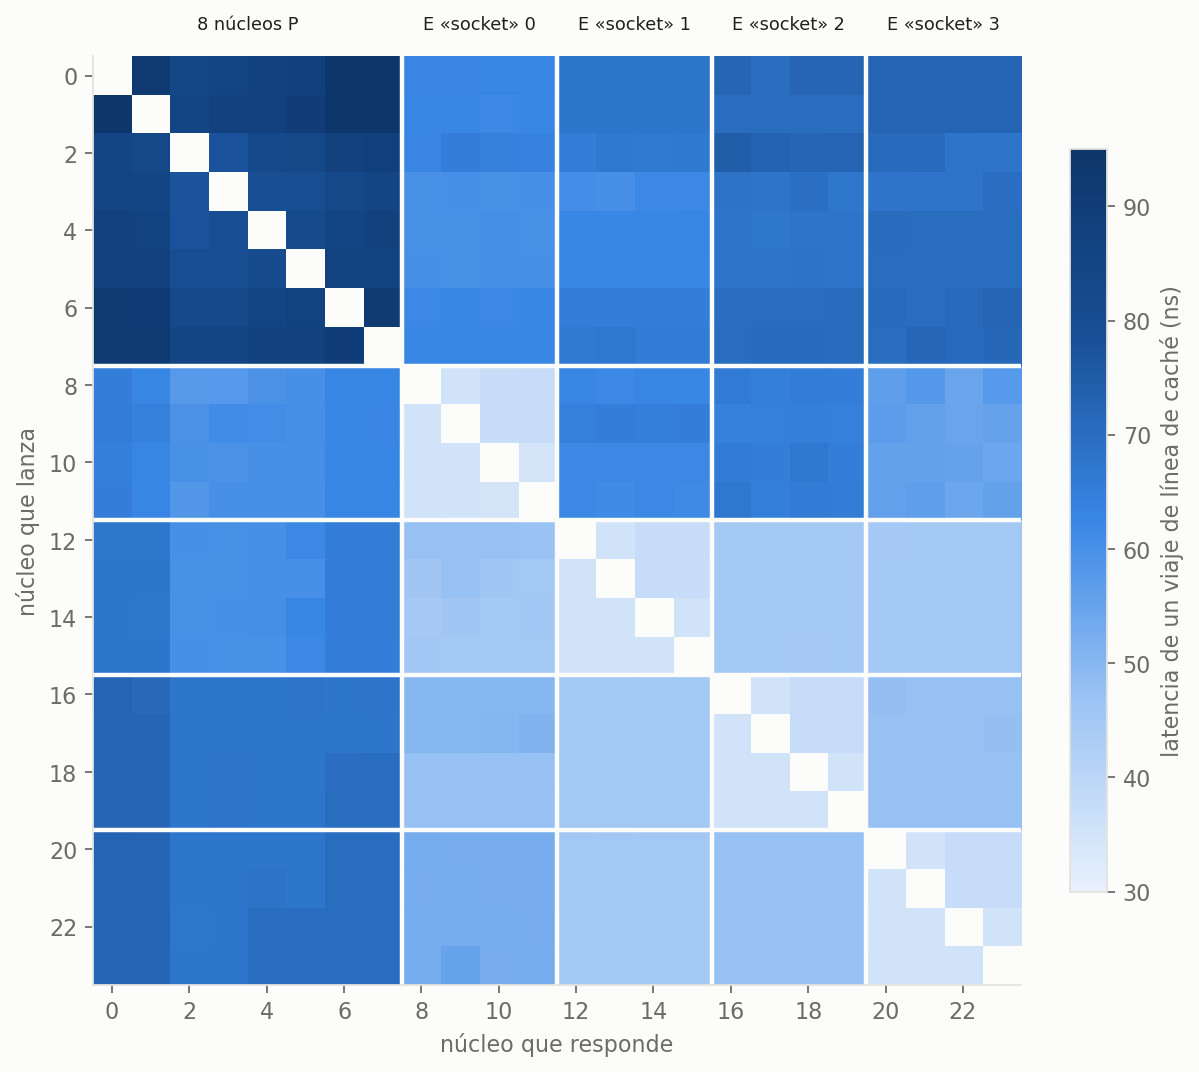
\includegraphics[width=\anchodisponible,height=148pt,keepaspectratio]{figuras/topologia.png}\par}}
\note{Figura original de la réplica, tal como la genera analizar.py a partir de los CSV de resultados/david-ultra9-285/. Se explica en la Parte 5.2 de EXPLICACION.md, donde viene también cómo leerla. Úsenla de respaldo en el turno de preguntas.}
\end{frame}}

{\fondo{cF7F4EC}\renewcommand\colorpie{c5F6B7A}\renewcommand\piediapo{\texttt{figuras/fig5\_replica.png} · generada por analizar.py · se explica en EXPLICACION.md, Parte 6.1}\renewcommand\titulonota{Rendimiento de las 5 implementaciones en los 6 escenarios}
\begin{frame}[plain]
\colocar{t}{{\fontsize{5.69}{7}\selectfont\bfseries\color{cB04A06}\MakeUppercase{Anexo · figura 2 de 20}\par}\vspace{6pt}{\fontsize{11.4}{13.1}\selectfont\bfseries\color{c14213D}\raggedright Rendimiento de las 5 implementaciones en los 6 escenarios\par}\vspace{8pt}{\centering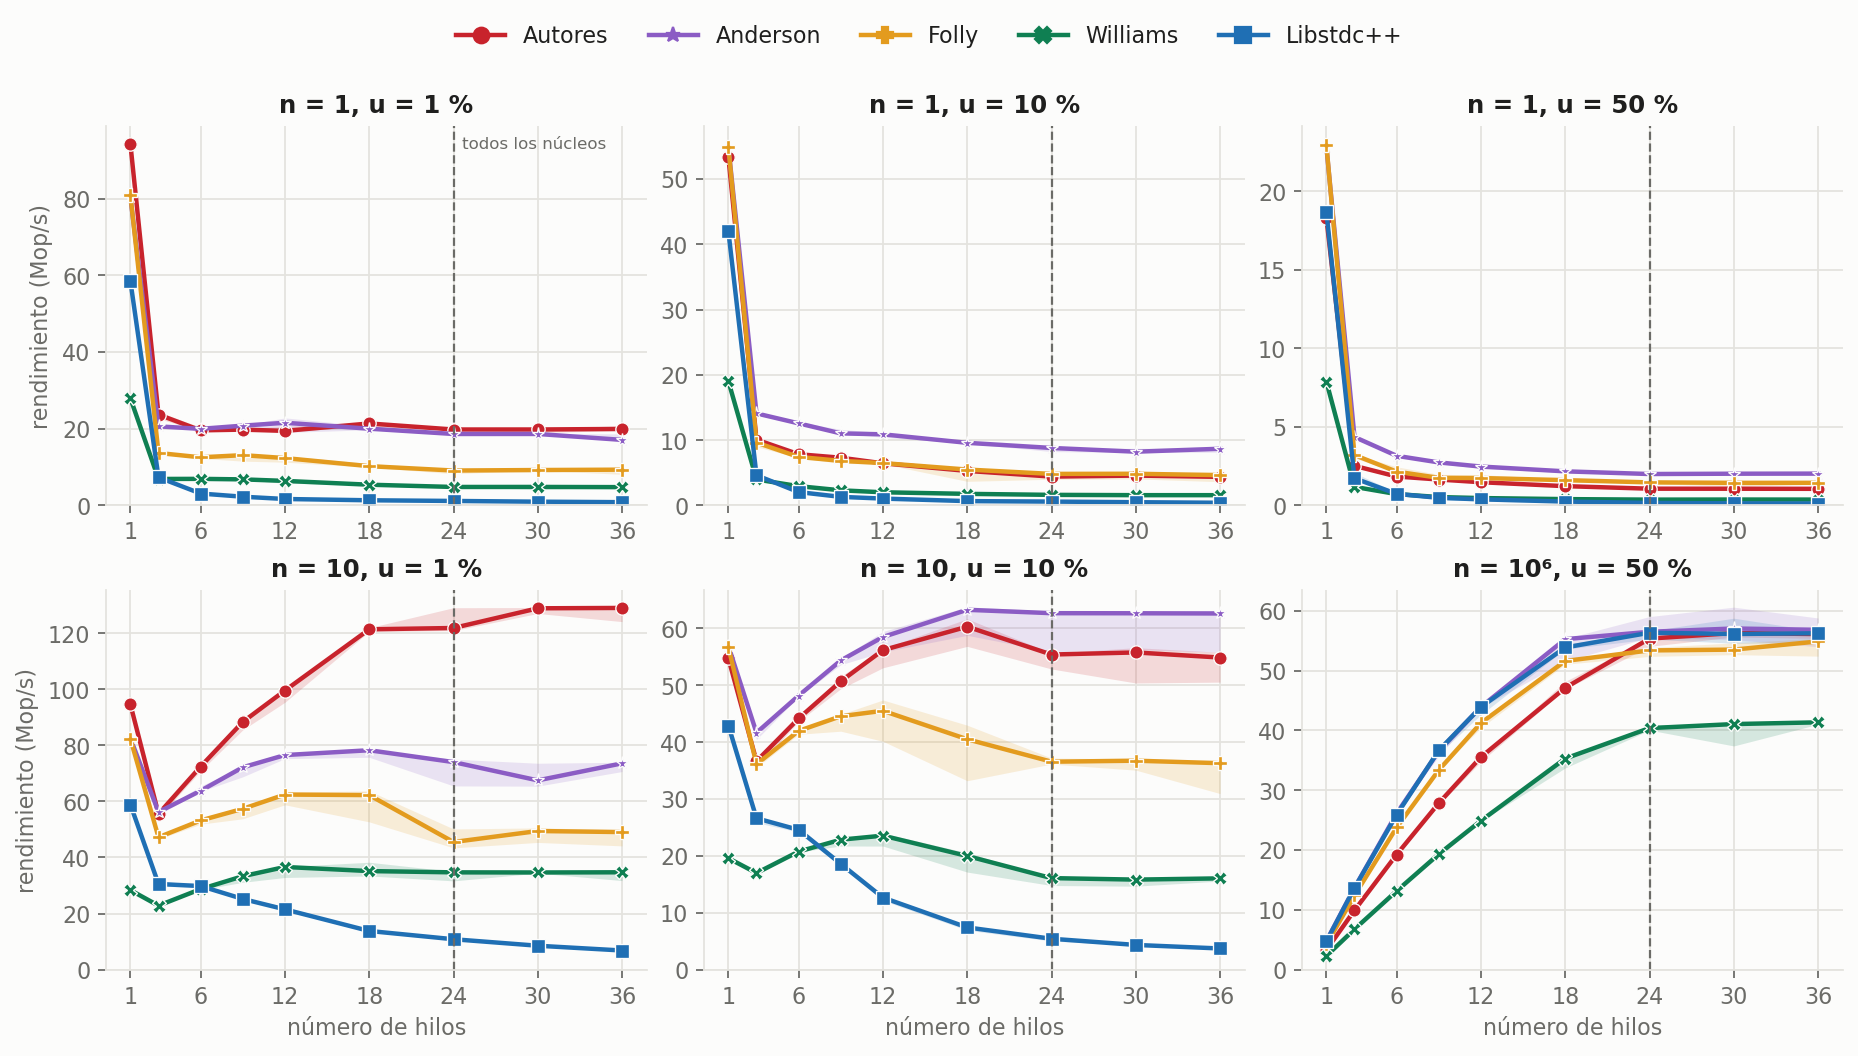
\includegraphics[width=\anchodisponible,height=148pt,keepaspectratio]{figuras/fig5_replica.png}\par}}
\note{Figura original de la réplica, tal como la genera analizar.py a partir de los CSV de resultados/david-ultra9-285/. Se explica en la Parte 6.1 de EXPLICACION.md, donde viene también cómo leerla. Úsenla de respaldo en el turno de preguntas.}
\end{frame}}

{\fondo{cF7F4EC}\renewcommand\colorpie{c5F6B7A}\renewcommand\piediapo{\texttt{figuras/fig5\_paper\_frente\_a\_replica.png} · generada por analizar.py · se explica en EXPLICACION.md, Parte 6.1}\renewcommand\titulonota{Cuánto rinde cada rival respecto a Autores, en el paper y en la réplica}
\begin{frame}[plain]
\colocar{t}{{\fontsize{5.69}{7}\selectfont\bfseries\color{cB04A06}\MakeUppercase{Anexo · figura 3 de 20}\par}\vspace{6pt}{\fontsize{11.4}{13.1}\selectfont\bfseries\color{c14213D}\raggedright Cuánto rinde cada rival respecto a Autores, en el paper y en la réplica\par}\vspace{8pt}{\centering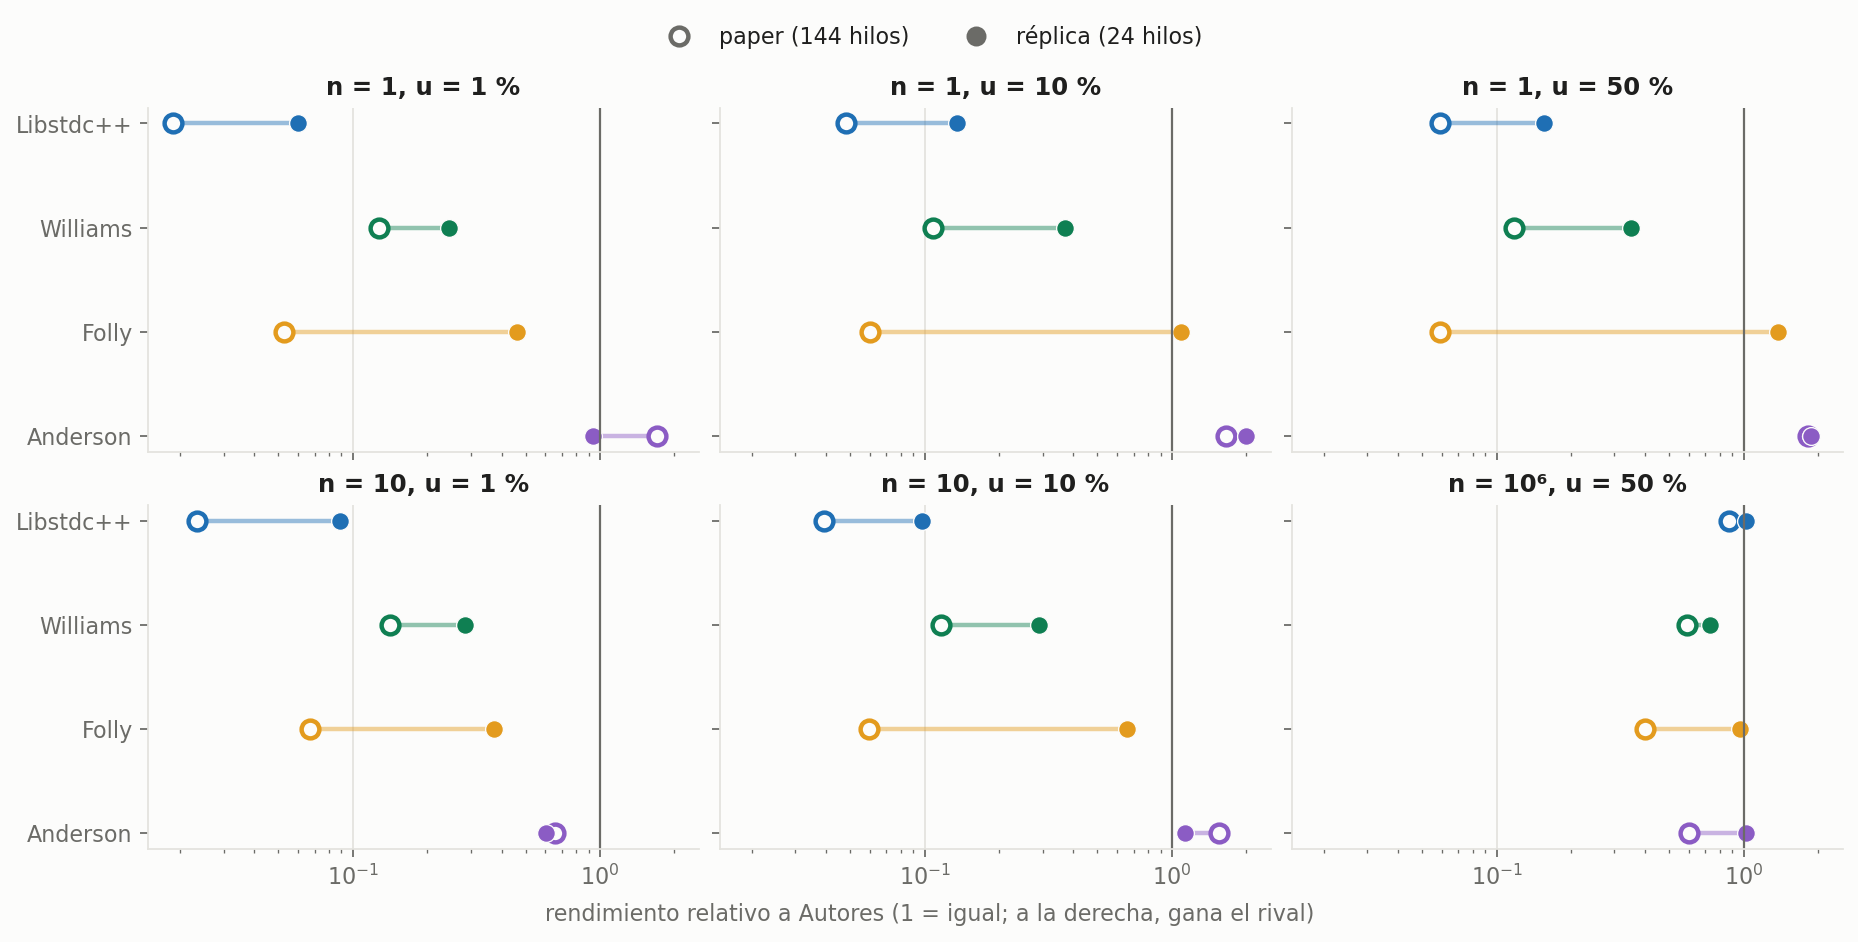
\includegraphics[width=\anchodisponible,height=148pt,keepaspectratio]{figuras/fig5_paper_frente_a_replica.png}\par}}
\note{Figura original de la réplica, tal como la genera analizar.py a partir de los CSV de resultados/david-ultra9-285/. Se explica en la Parte 6.1 de EXPLICACION.md, donde viene también cómo leerla. Úsenla de respaldo en el turno de preguntas.}
\end{frame}}

{\fondo{cF7F4EC}\renewcommand\colorpie{c5F6B7A}\renewcommand\piediapo{\texttt{figuras/memoria\_ram.png} · generada por analizar.py · se explica en EXPLICACION.md, Parte 6.1}\renewcommand\titulonota{Tráfico real de RAM}
\begin{frame}[plain]
\colocar{t}{{\fontsize{5.69}{7}\selectfont\bfseries\color{cB04A06}\MakeUppercase{Anexo · figura 4 de 20}\par}\vspace{6pt}{\fontsize{11.4}{13.1}\selectfont\bfseries\color{c14213D}\raggedright Tráfico real de RAM\par}\vspace{8pt}{\centering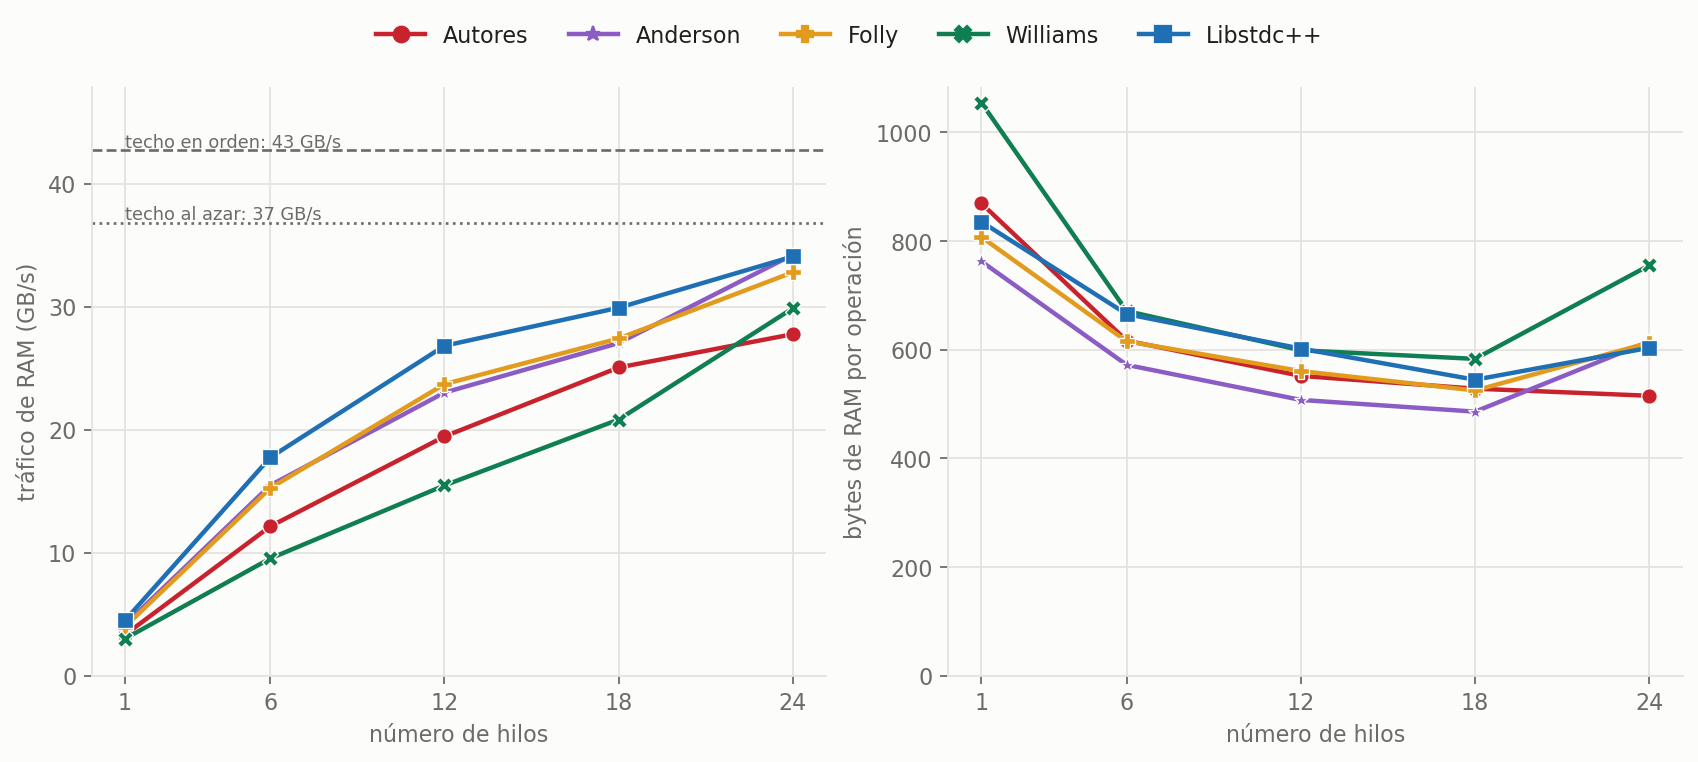
\includegraphics[width=\anchodisponible,height=148pt,keepaspectratio]{figuras/memoria_ram.png}\par}}
\note{Figura original de la réplica, tal como la genera analizar.py a partir de los CSV de resultados/david-ultra9-285/. Se explica en la Parte 6.1 de EXPLICACION.md, donde viene también cómo leerla. Úsenla de respaldo en el turno de preguntas.}
\end{frame}}

{\fondo{cF7F4EC}\renewcommand\colorpie{c5F6B7A}\renewcommand\piediapo{\texttt{figuras/fig6\_replica.png} · generada por analizar.py · se explica en EXPLICACION.md, Parte 6.2}\renewcommand\titulonota{Latencia de cada operación con y sin contención}
\begin{frame}[plain]
\colocar{t}{{\fontsize{5.69}{7}\selectfont\bfseries\color{cB04A06}\MakeUppercase{Anexo · figura 5 de 20}\par}\vspace{6pt}{\fontsize{11.4}{13.1}\selectfont\bfseries\color{c14213D}\raggedright Latencia de cada operación con y sin contención\par}\vspace{8pt}{\centering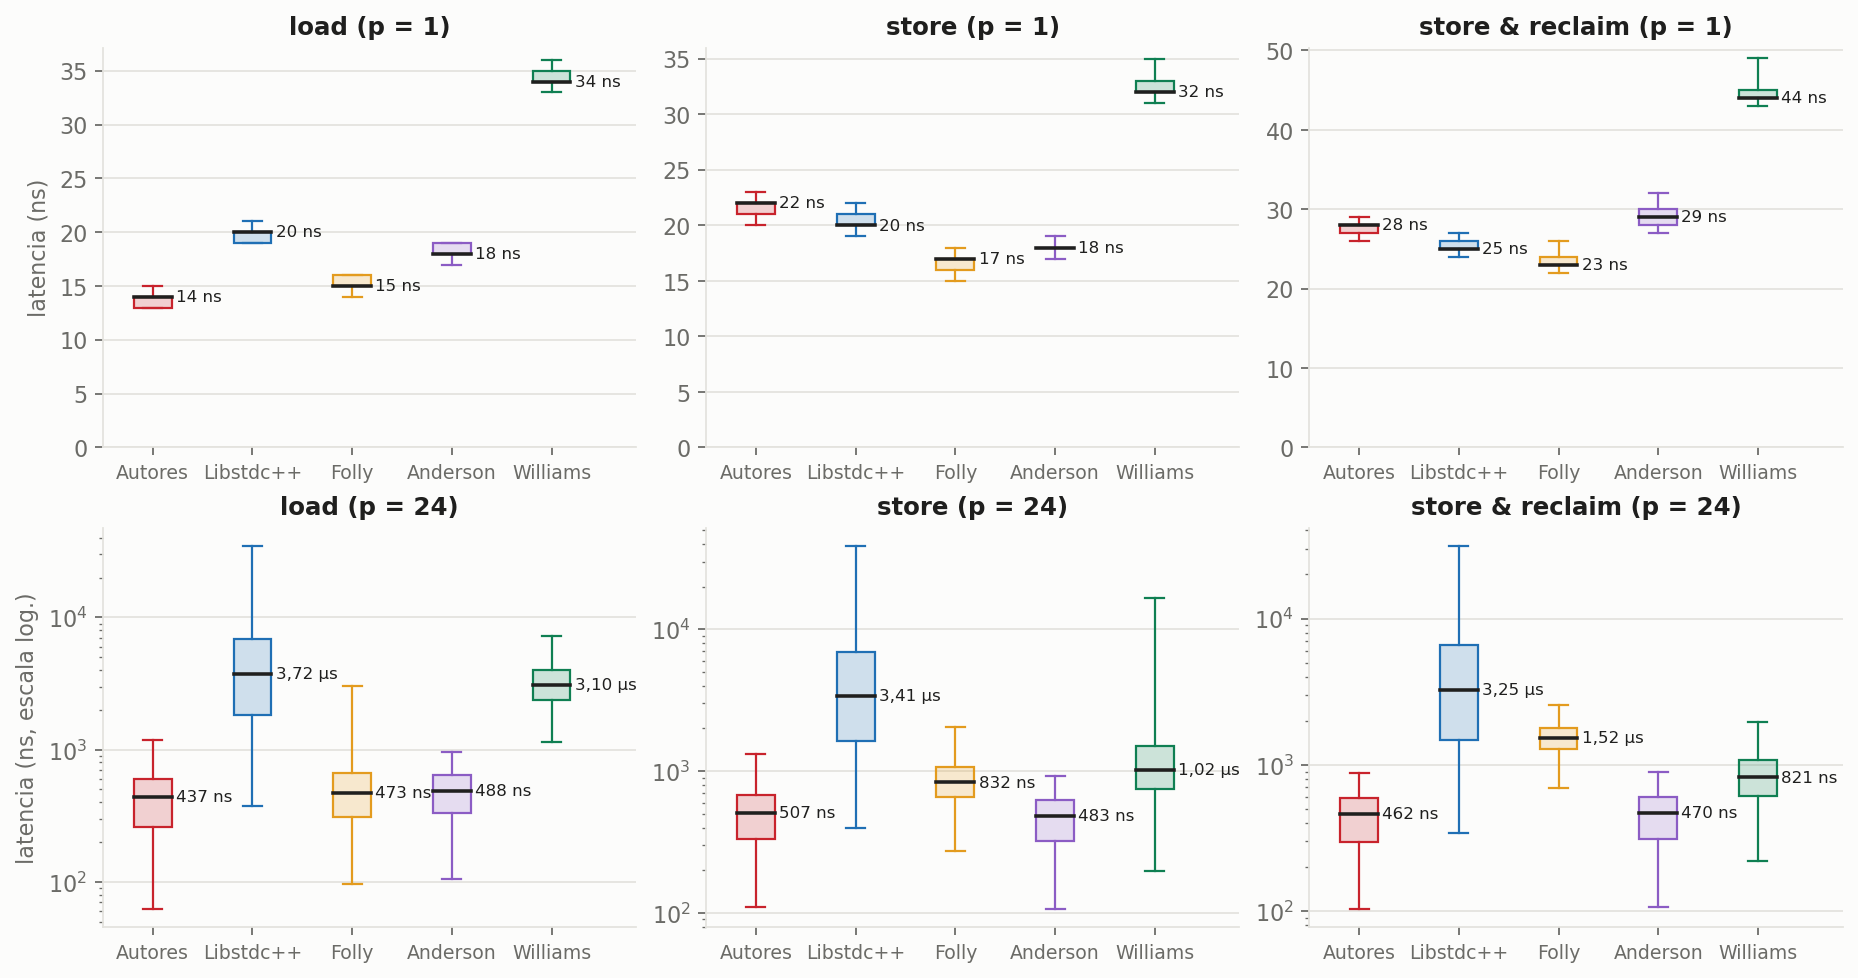
\includegraphics[width=\anchodisponible,height=148pt,keepaspectratio]{figuras/fig6_replica.png}\par}}
\note{Figura original de la réplica, tal como la genera analizar.py a partir de los CSV de resultados/david-ultra9-285/. Se explica en la Parte 6.2 de EXPLICACION.md, donde viene también cómo leerla. Úsenla de respaldo en el turno de preguntas.}
\end{frame}}

{\fondo{cF7F4EC}\renewcommand\colorpie{c5F6B7A}\renewcommand\piediapo{\texttt{figuras/nativo\_oficial\_fig6.png} · generada por analizar.py · se explica en EXPLICACION.md, Parte 6.2}\renewcommand\titulonota{Latencia sin Docker con los programas oficiales}
\begin{frame}[plain]
\colocar{t}{{\fontsize{5.69}{7}\selectfont\bfseries\color{cB04A06}\MakeUppercase{Anexo · figura 6 de 20}\par}\vspace{6pt}{\fontsize{11.4}{13.1}\selectfont\bfseries\color{c14213D}\raggedright Latencia sin Docker con los programas oficiales\par}\vspace{8pt}{\centering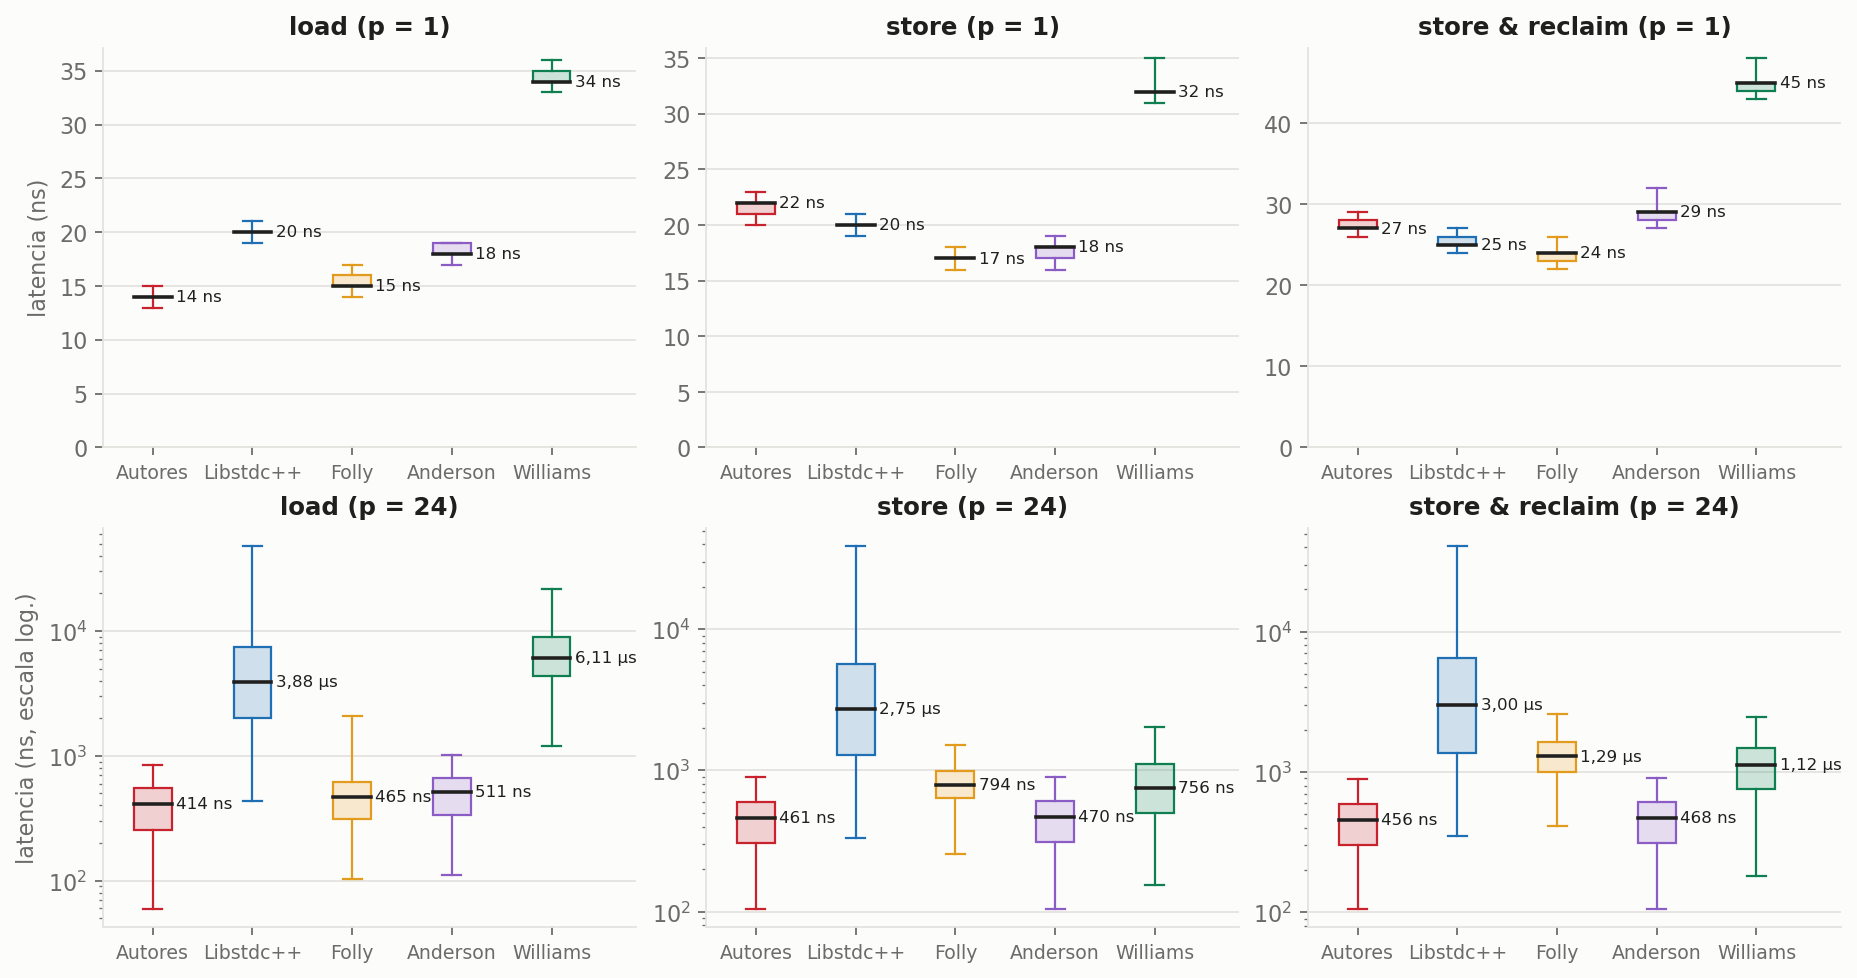
\includegraphics[width=\anchodisponible,height=148pt,keepaspectratio]{figuras/nativo_oficial_fig6.png}\par}}
\note{Figura original de la réplica, tal como la genera analizar.py a partir de los CSV de resultados/david-ultra9-285/. Se explica en la Parte 6.2 de EXPLICACION.md, donde viene también cómo leerla. Úsenla de respaldo en el turno de preguntas.}
\end{frame}}

{\fondo{cF7F4EC}\renewcommand\colorpie{c5F6B7A}\renewcommand\piediapo{\texttt{figuras/memoria\_retenida.png} · generada por analizar.py · se explica en EXPLICACION.md, Parte 6.3}\renewcommand\titulonota{Pico de bloques de memoria vivos}
\begin{frame}[plain]
\colocar{t}{{\fontsize{5.69}{7}\selectfont\bfseries\color{cB04A06}\MakeUppercase{Anexo · figura 7 de 20}\par}\vspace{6pt}{\fontsize{11.4}{13.1}\selectfont\bfseries\color{c14213D}\raggedright Pico de bloques de memoria vivos\par}\vspace{8pt}{\centering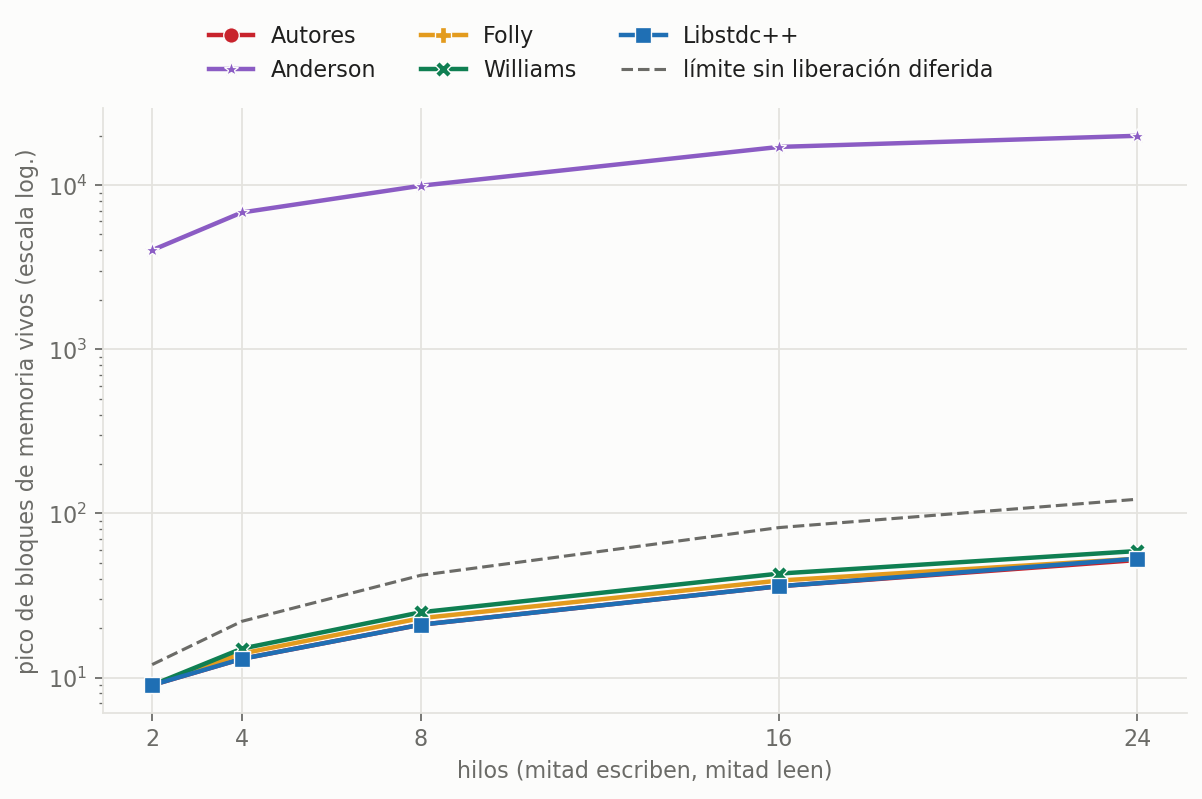
\includegraphics[width=\anchodisponible,height=148pt,keepaspectratio]{figuras/memoria_retenida.png}\par}}
\note{Figura original de la réplica, tal como la genera analizar.py a partir de los CSV de resultados/david-ultra9-285/. Se explica en la Parte 6.3 de EXPLICACION.md, donde viene también cómo leerla. Úsenla de respaldo en el turno de preguntas.}
\end{frame}}

{\fondo{cF7F4EC}\renewcommand\colorpie{c5F6B7A}\renewcommand\piediapo{\texttt{figuras/nativo\_oficial\_memoria\_retenida.png} · generada por analizar.py · se explica en EXPLICACION.md, Parte 6.3}\renewcommand\titulonota{Pico de bloques de memoria vivos, sin Docker}
\begin{frame}[plain]
\colocar{t}{{\fontsize{5.69}{7}\selectfont\bfseries\color{cB04A06}\MakeUppercase{Anexo · figura 8 de 20}\par}\vspace{6pt}{\fontsize{11.4}{13.1}\selectfont\bfseries\color{c14213D}\raggedright Pico de bloques de memoria vivos, sin Docker\par}\vspace{8pt}{\centering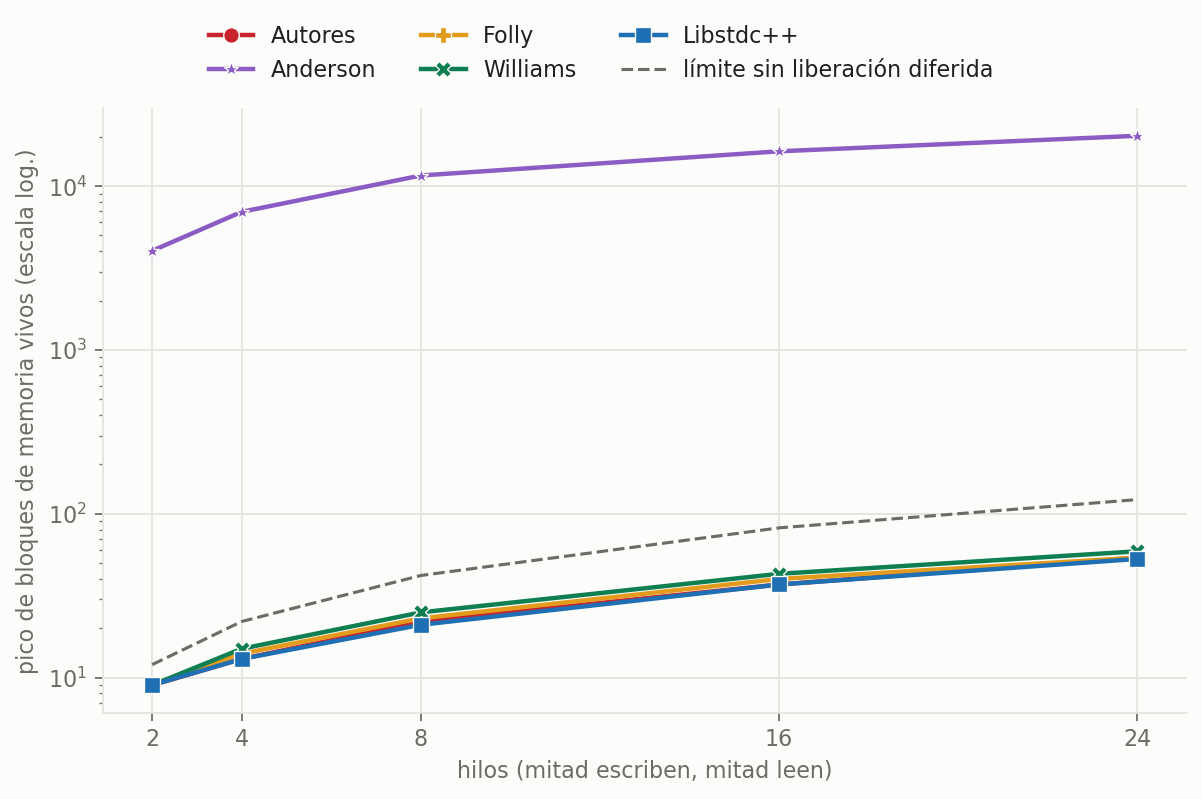
\includegraphics[width=\anchodisponible,height=148pt,keepaspectratio]{figuras/nativo_oficial_memoria_retenida.png}\par}}
\note{Figura original de la réplica, tal como la genera analizar.py a partir de los CSV de resultados/david-ultra9-285/. Se explica en la Parte 6.3 de EXPLICACION.md, donde viene también cómo leerla. Úsenla de respaldo en el turno de preguntas.}
\end{frame}}

{\fondo{cF7F4EC}\renewcommand\colorpie{c5F6B7A}\renewcommand\piediapo{\texttt{figuras/afinidad\_dosis\_respuesta.png} · generada por analizar.py · se explica en EXPLICACION.md, Parte 6.4}\renewcommand\titulonota{Rendimiento con 4 hilos a distancia creciente}
\begin{frame}[plain]
\colocar{t}{{\fontsize{5.69}{7}\selectfont\bfseries\color{cB04A06}\MakeUppercase{Anexo · figura 9 de 20}\par}\vspace{6pt}{\fontsize{11.4}{13.1}\selectfont\bfseries\color{c14213D}\raggedright Rendimiento con 4 hilos a distancia creciente\par}\vspace{8pt}{\centering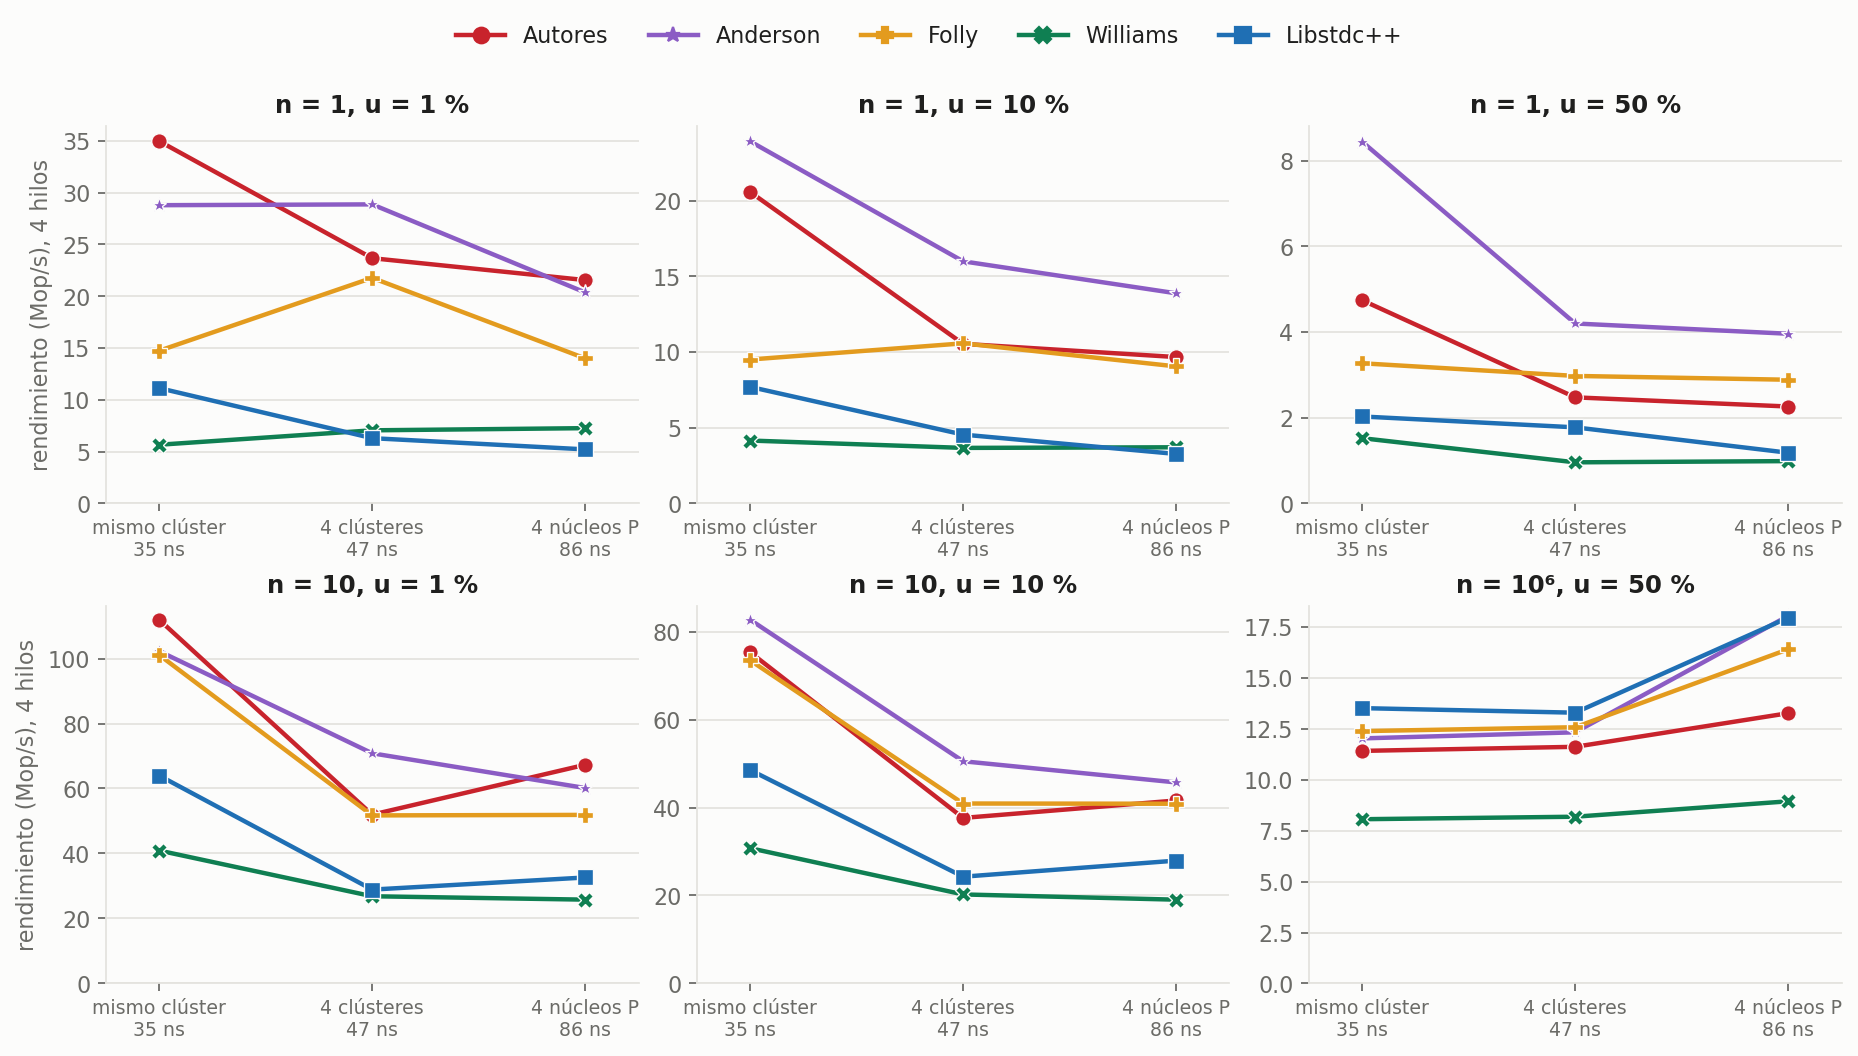
\includegraphics[width=\anchodisponible,height=148pt,keepaspectratio]{figuras/afinidad_dosis_respuesta.png}\par}}
\note{Figura original de la réplica, tal como la genera analizar.py a partir de los CSV de resultados/david-ultra9-285/. Se explica en la Parte 6.4 de EXPLICACION.md, donde viene también cómo leerla. Úsenla de respaldo en el turno de preguntas.}
\end{frame}}

{\fondo{cF7F4EC}\renewcommand\colorpie{c5F6B7A}\renewcommand\piediapo{\texttt{figuras/afinidad\_mapa\_4hilos.png} · generada por analizar.py · se explica en EXPLICACION.md, Parte 6.4}\renewcommand\titulonota{Cambio de rendimiento al separar 4 hilos}
\begin{frame}[plain]
\colocar{t}{{\fontsize{5.69}{7}\selectfont\bfseries\color{cB04A06}\MakeUppercase{Anexo · figura 10 de 20}\par}\vspace{6pt}{\fontsize{11.4}{13.1}\selectfont\bfseries\color{c14213D}\raggedright Cambio de rendimiento al separar 4 hilos\par}\vspace{8pt}{\centering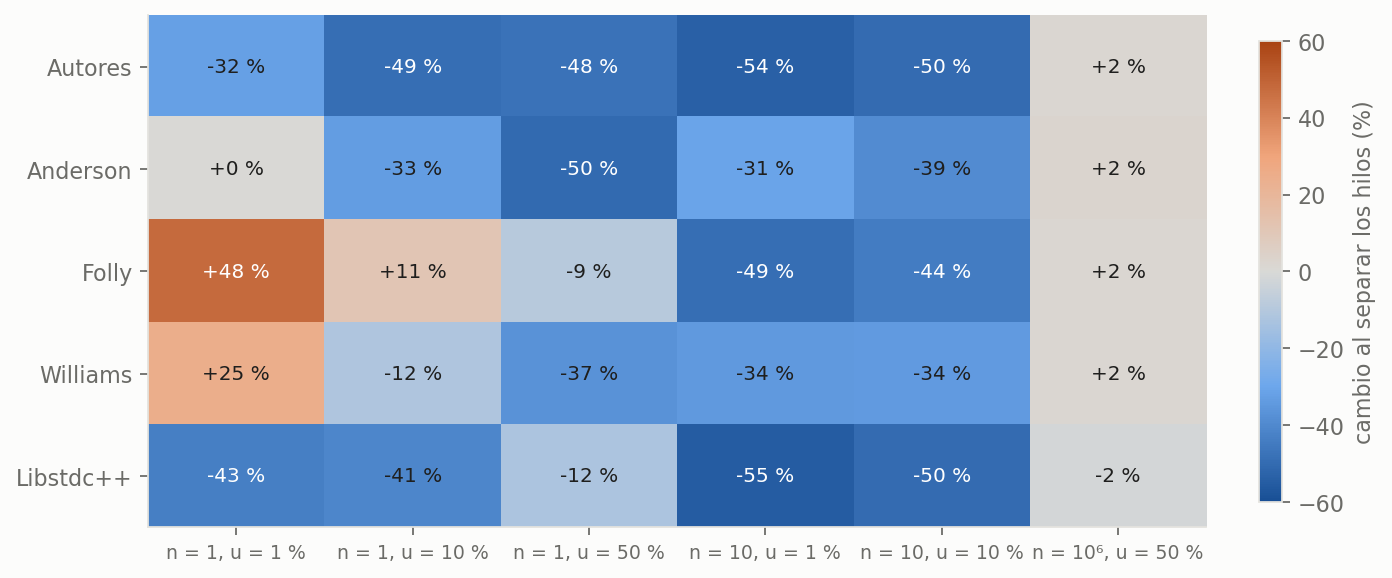
\includegraphics[width=\anchodisponible,height=148pt,keepaspectratio]{figuras/afinidad_mapa_4hilos.png}\par}}
\note{Figura original de la réplica, tal como la genera analizar.py a partir de los CSV de resultados/david-ultra9-285/. Se explica en la Parte 6.4 de EXPLICACION.md, donde viene también cómo leerla. Úsenla de respaldo en el turno de preguntas.}
\end{frame}}

{\fondo{cF7F4EC}\renewcommand\colorpie{c5F6B7A}\renewcommand\piediapo{\texttt{figuras/nativo\_oficial\_dosis\_respuesta.png} · generada por analizar.py · se explica en EXPLICACION.md, Parte 6.4}\renewcommand\titulonota{Rendimiento con 4 hilos a distancia creciente, sin Docker y con los programas oficiales}
\begin{frame}[plain]
\colocar{t}{{\fontsize{5.69}{7}\selectfont\bfseries\color{cB04A06}\MakeUppercase{Anexo · figura 11 de 20}\par}\vspace{6pt}{\fontsize{11.4}{13.1}\selectfont\bfseries\color{c14213D}\raggedright Rendimiento con 4 hilos a distancia creciente, sin Docker y con los programas oficiales\par}\vspace{8pt}{\centering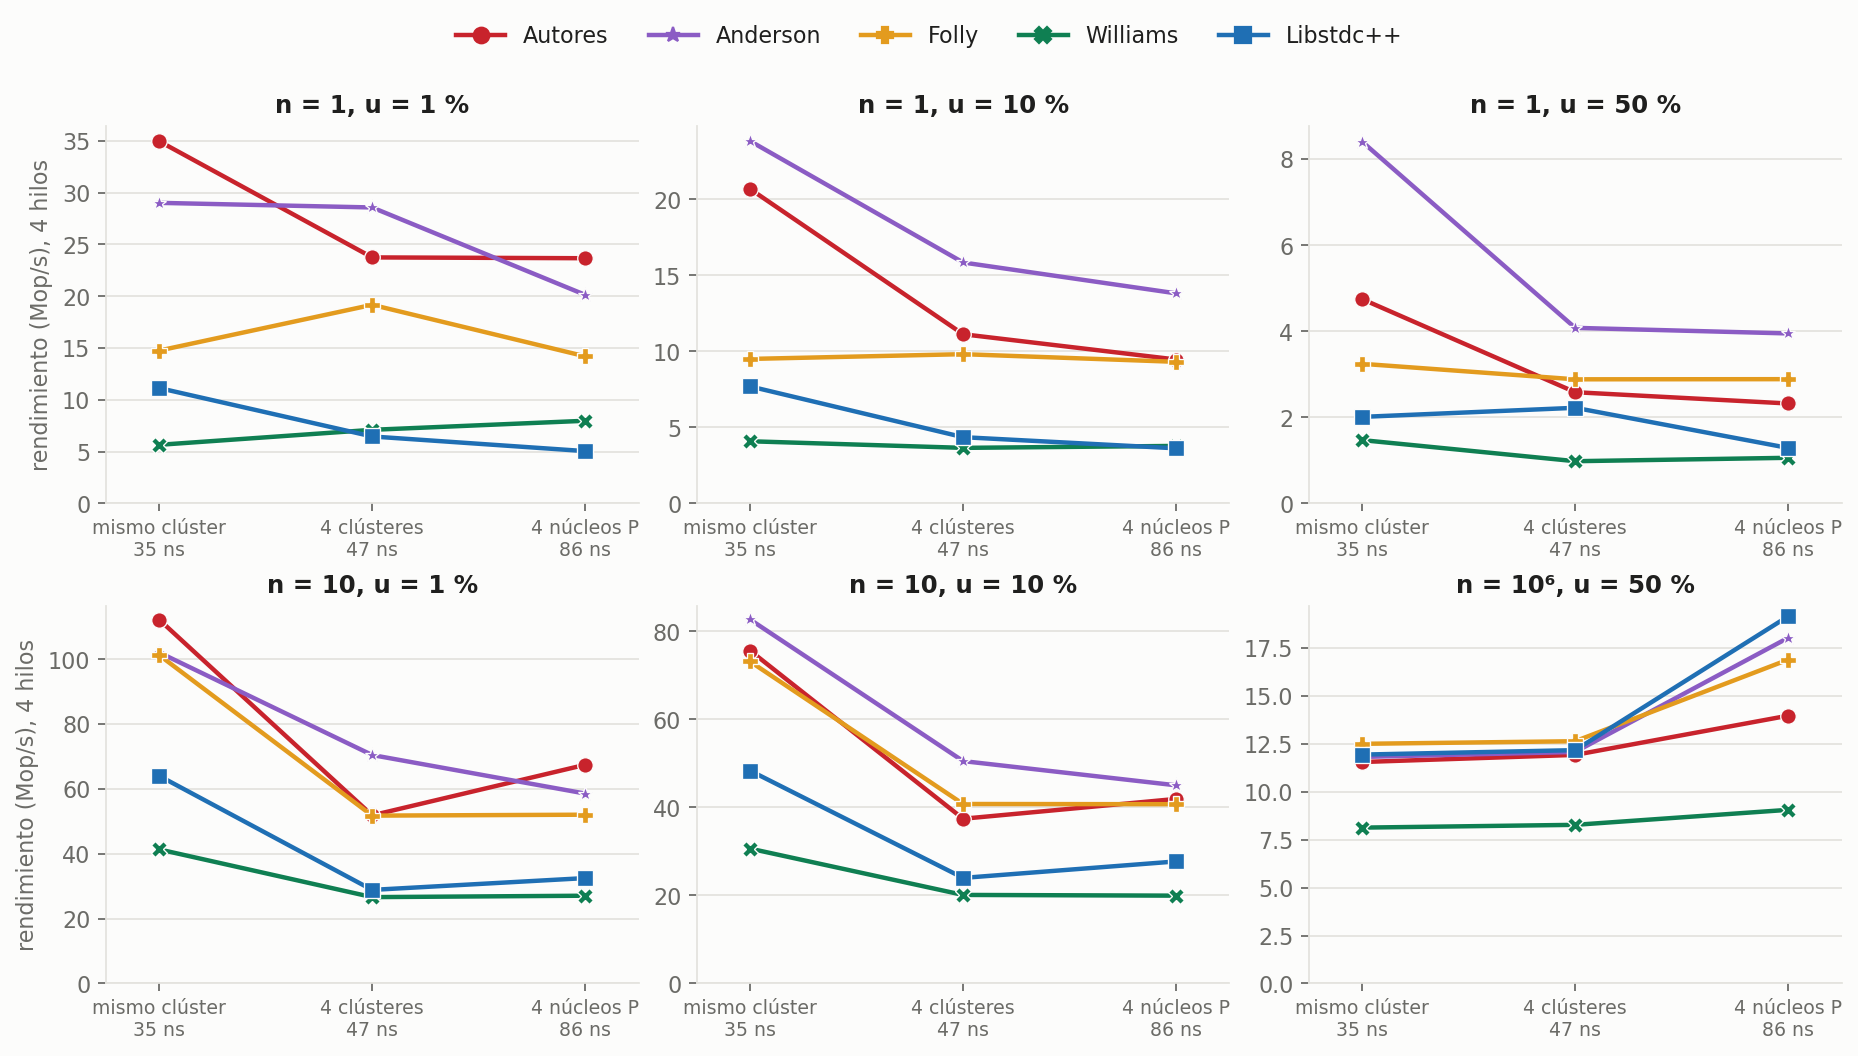
\includegraphics[width=\anchodisponible,height=148pt,keepaspectratio]{figuras/nativo_oficial_dosis_respuesta.png}\par}}
\note{Figura original de la réplica, tal como la genera analizar.py a partir de los CSV de resultados/david-ultra9-285/. Se explica en la Parte 6.4 de EXPLICACION.md, donde viene también cómo leerla. Úsenla de respaldo en el turno de preguntas.}
\end{frame}}

{\fondo{cF7F4EC}\renewcommand\colorpie{c5F6B7A}\renewcommand\piediapo{\texttt{figuras/afinidad\_mapa\_8hilos.png} · generada por analizar.py · se explica en EXPLICACION.md, Parte 6.4}\renewcommand\titulonota{Cambio de rendimiento al separar 8 hilos}
\begin{frame}[plain]
\colocar{t}{{\fontsize{5.69}{7}\selectfont\bfseries\color{cB04A06}\MakeUppercase{Anexo · figura 12 de 20}\par}\vspace{6pt}{\fontsize{11.4}{13.1}\selectfont\bfseries\color{c14213D}\raggedright Cambio de rendimiento al separar 8 hilos\par}\vspace{8pt}{\centering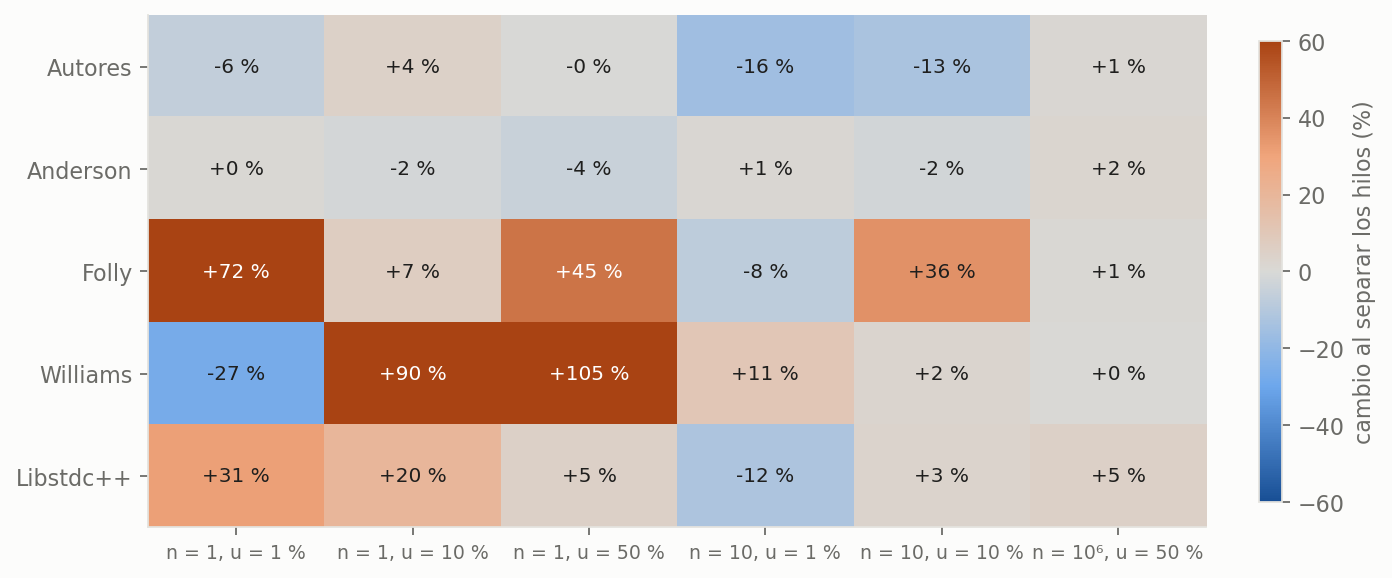
\includegraphics[width=\anchodisponible,height=148pt,keepaspectratio]{figuras/afinidad_mapa_8hilos.png}\par}}
\note{Figura original de la réplica, tal como la genera analizar.py a partir de los CSV de resultados/david-ultra9-285/. Se explica en la Parte 6.4 de EXPLICACION.md, donde viene también cómo leerla. Úsenla de respaldo en el turno de preguntas.}
\end{frame}}

{\fondo{cF7F4EC}\renewcommand\colorpie{c5F6B7A}\renewcommand\piediapo{\texttt{figuras/miniatura\_frente\_a\_paper.png} · generada por analizar.py · se explica en EXPLICACION.md, Parte 6.4}\renewcommand\titulonota{Paper y réplica según el porcentaje de núcleos en uso}
\begin{frame}[plain]
\colocar{t}{{\fontsize{5.69}{7}\selectfont\bfseries\color{cB04A06}\MakeUppercase{Anexo · figura 13 de 20}\par}\vspace{6pt}{\fontsize{11.4}{13.1}\selectfont\bfseries\color{c14213D}\raggedright Paper y réplica según el porcentaje de núcleos en uso\par}\vspace{8pt}{\centering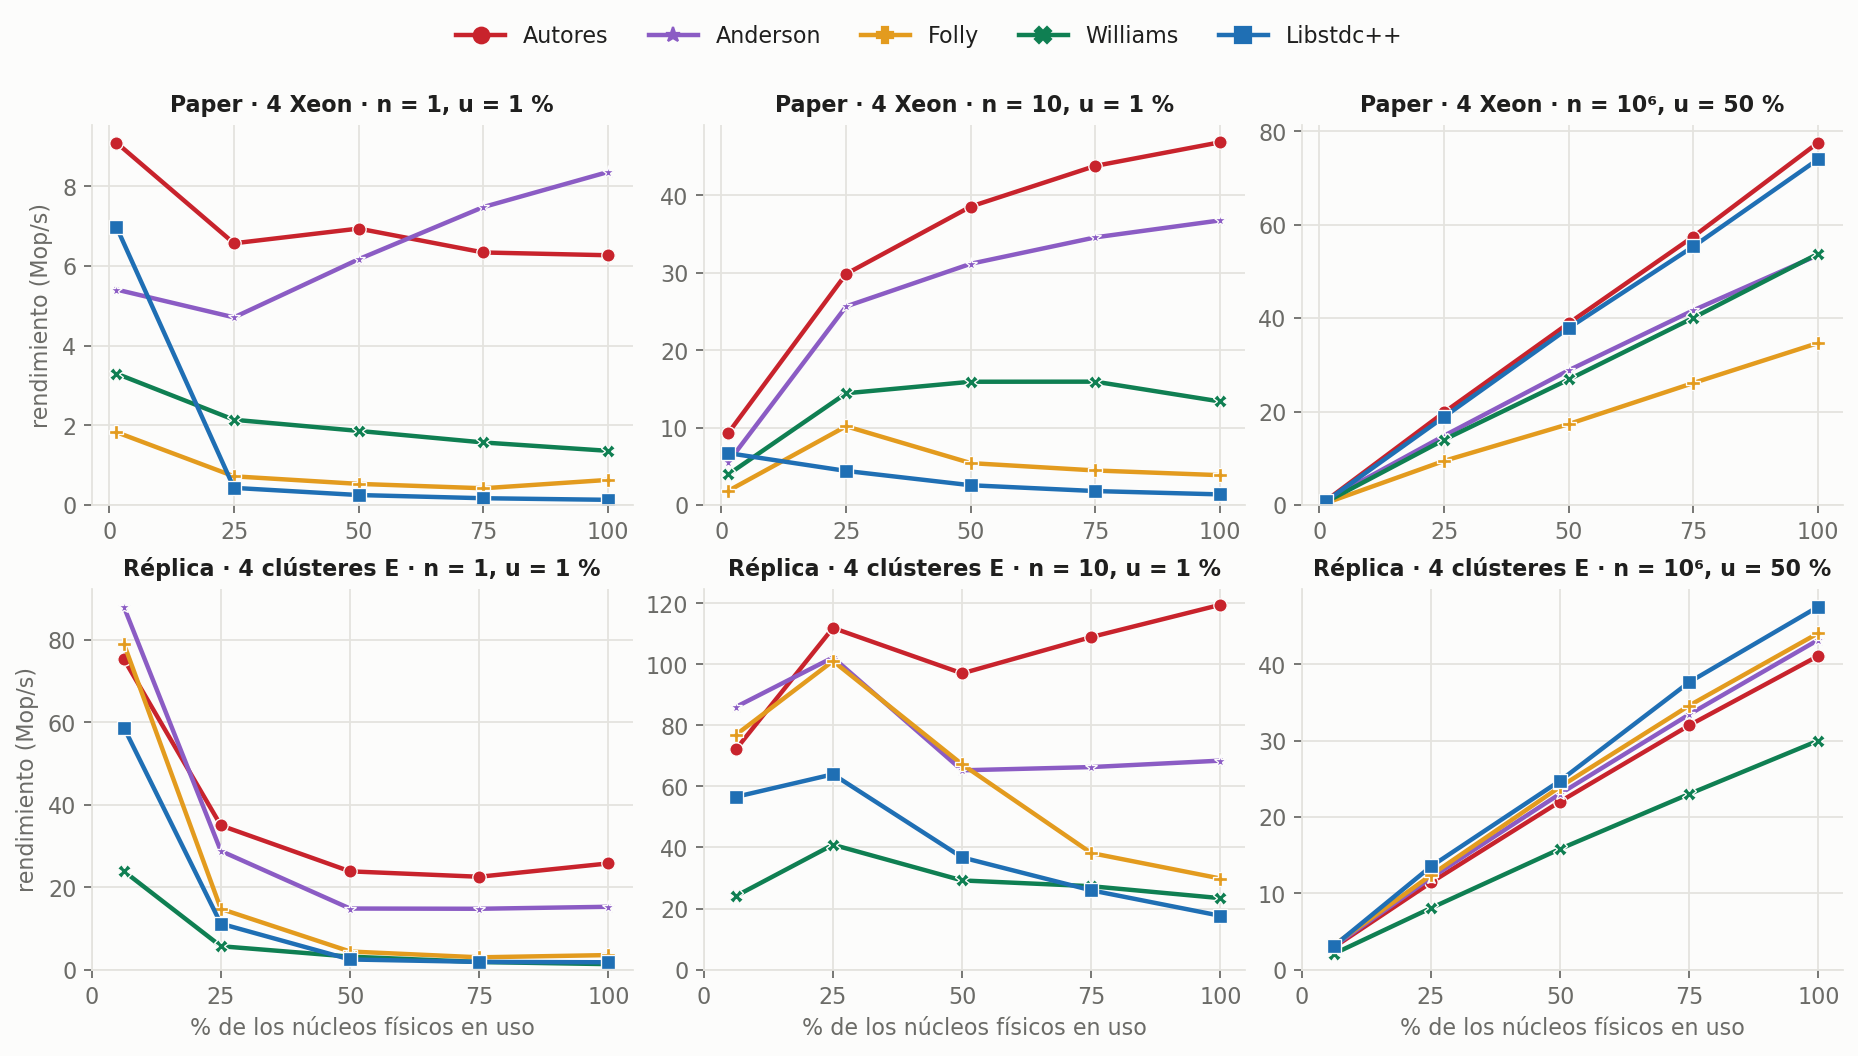
\includegraphics[width=\anchodisponible,height=148pt,keepaspectratio]{figuras/miniatura_frente_a_paper.png}\par}}
\note{Figura original de la réplica, tal como la genera analizar.py a partir de los CSV de resultados/david-ultra9-285/. Se explica en la Parte 6.4 de EXPLICACION.md, donde viene también cómo leerla. Úsenla de respaldo en el turno de preguntas.}
\end{frame}}

{\fondo{cF7F4EC}\renewcommand\colorpie{c5F6B7A}\renewcommand\piediapo{\texttt{figuras/docker\_frente\_a\_nativo\_oficial.png} · generada por analizar.py · se explica en EXPLICACION.md, Parte 6.6}\renewcommand\titulonota{Cada punto de la figura 5 con los programas oficiales, con Docker y sin Docker}
\begin{frame}[plain]
\colocar{t}{{\fontsize{5.69}{7}\selectfont\bfseries\color{cB04A06}\MakeUppercase{Anexo · figura 14 de 20}\par}\vspace{6pt}{\fontsize{11.4}{13.1}\selectfont\bfseries\color{c14213D}\raggedright Cada punto de la figura 5 con los programas oficiales, con Docker y sin Docker\par}\vspace{8pt}{\centering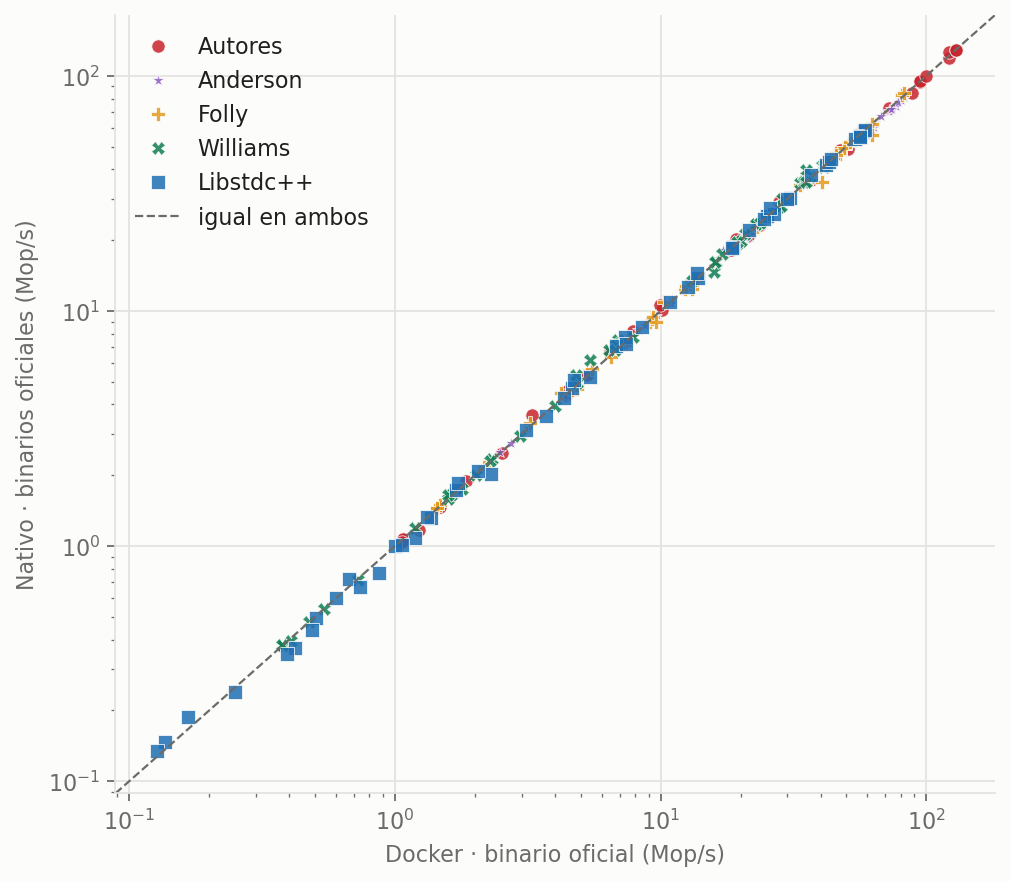
\includegraphics[width=\anchodisponible,height=148pt,keepaspectratio]{figuras/docker_frente_a_nativo_oficial.png}\par}}
\note{Figura original de la réplica, tal como la genera analizar.py a partir de los CSV de resultados/david-ultra9-285/. Se explica en la Parte 6.6 de EXPLICACION.md, donde viene también cómo leerla. Úsenla de respaldo en el turno de preguntas.}
\end{frame}}

{\fondo{cF7F4EC}\renewcommand\colorpie{c5F6B7A}\renewcommand\piediapo{\texttt{figuras/nativo\_oficial\_fig5.png} · generada por analizar.py · se explica en EXPLICACION.md, Parte 6.6}\renewcommand\titulonota{Rendimiento sin Docker con los programas oficiales}
\begin{frame}[plain]
\colocar{t}{{\fontsize{5.69}{7}\selectfont\bfseries\color{cB04A06}\MakeUppercase{Anexo · figura 15 de 20}\par}\vspace{6pt}{\fontsize{11.4}{13.1}\selectfont\bfseries\color{c14213D}\raggedright Rendimiento sin Docker con los programas oficiales\par}\vspace{8pt}{\centering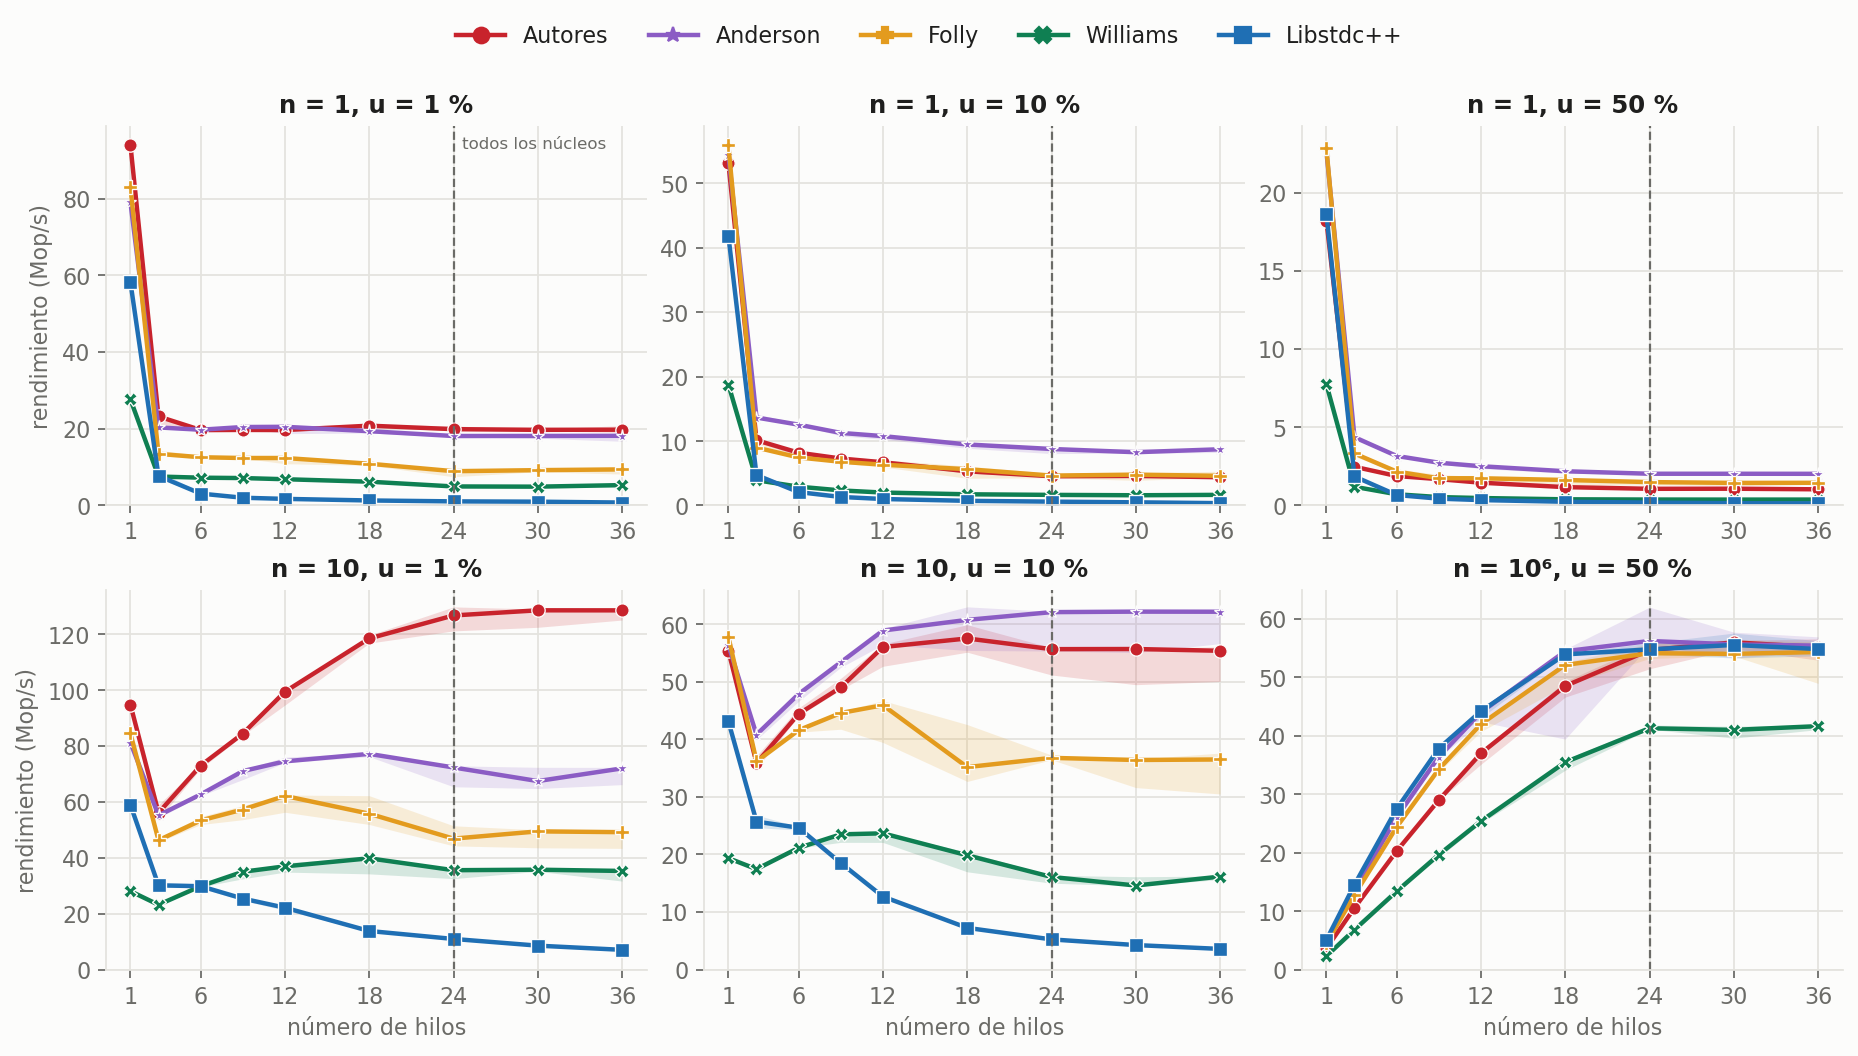
\includegraphics[width=\anchodisponible,height=148pt,keepaspectratio]{figuras/nativo_oficial_fig5.png}\par}}
\note{Figura original de la réplica, tal como la genera analizar.py a partir de los CSV de resultados/david-ultra9-285/. Se explica en la Parte 6.6 de EXPLICACION.md, donde viene también cómo leerla. Úsenla de respaldo en el turno de preguntas.}
\end{frame}}

{\fondo{cF7F4EC}\renewcommand\colorpie{c5F6B7A}\renewcommand\piediapo{\texttt{figuras/nativo\_fig5.png} · generada por analizar.py · se explica en EXPLICACION.md, Parte 6.6}\renewcommand\titulonota{Rendimiento sin Docker con bench.cpp del equipo}
\begin{frame}[plain]
\colocar{t}{{\fontsize{5.69}{7}\selectfont\bfseries\color{cB04A06}\MakeUppercase{Anexo · figura 16 de 20}\par}\vspace{6pt}{\fontsize{11.4}{13.1}\selectfont\bfseries\color{c14213D}\raggedright Rendimiento sin Docker con bench.cpp del equipo\par}\vspace{8pt}{\centering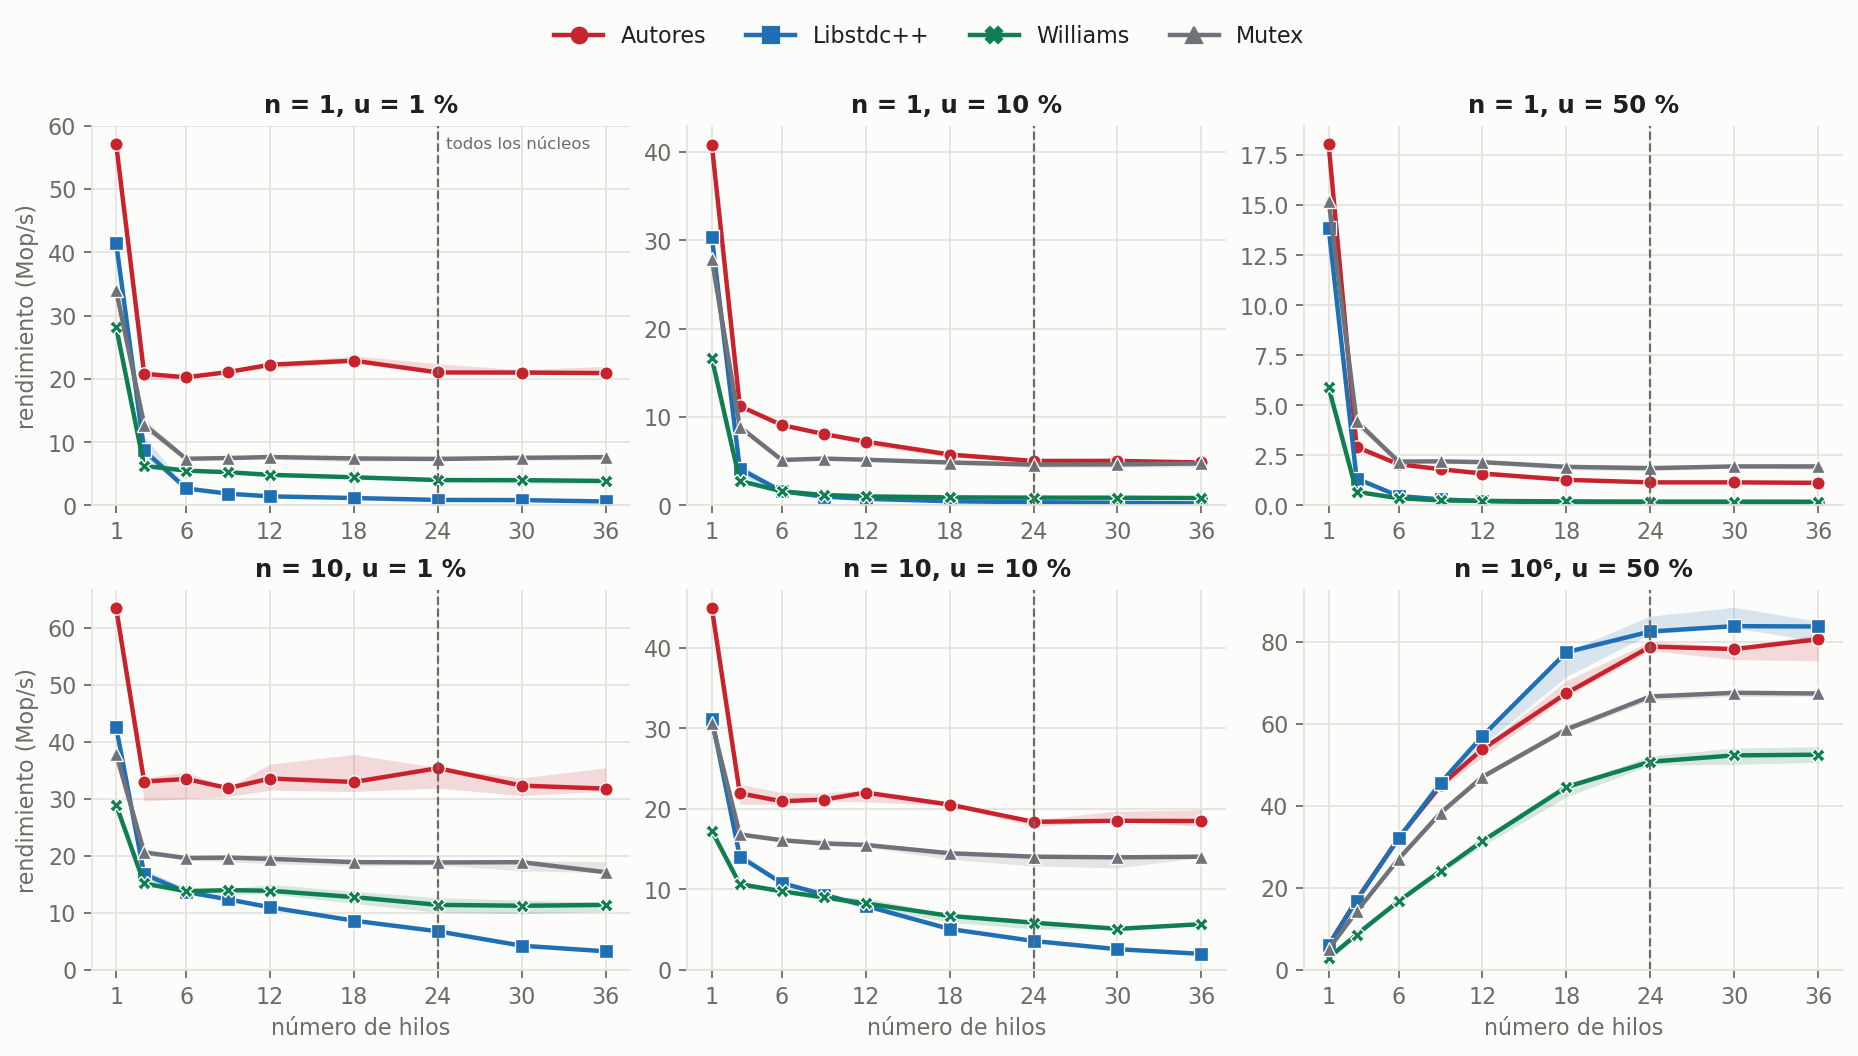
\includegraphics[width=\anchodisponible,height=148pt,keepaspectratio]{figuras/nativo_fig5.png}\par}}
\note{Figura original de la réplica, tal como la genera analizar.py a partir de los CSV de resultados/david-ultra9-285/. Se explica en la Parte 6.6 de EXPLICACION.md, donde viene también cómo leerla. Úsenla de respaldo en el turno de preguntas.}
\end{frame}}

{\fondo{cF7F4EC}\renewcommand\colorpie{c5F6B7A}\renewcommand\piediapo{\texttt{figuras/nativo\_alineado\_fig5.png} · generada por analizar.py · se explica en EXPLICACION.md, Parte 6.6}\renewcommand\titulonota{Rendimiento sin Docker con bench.cpp y las pilas alineadas}
\begin{frame}[plain]
\colocar{t}{{\fontsize{5.69}{7}\selectfont\bfseries\color{cB04A06}\MakeUppercase{Anexo · figura 17 de 20}\par}\vspace{6pt}{\fontsize{11.4}{13.1}\selectfont\bfseries\color{c14213D}\raggedright Rendimiento sin Docker con bench.cpp y las pilas alineadas\par}\vspace{8pt}{\centering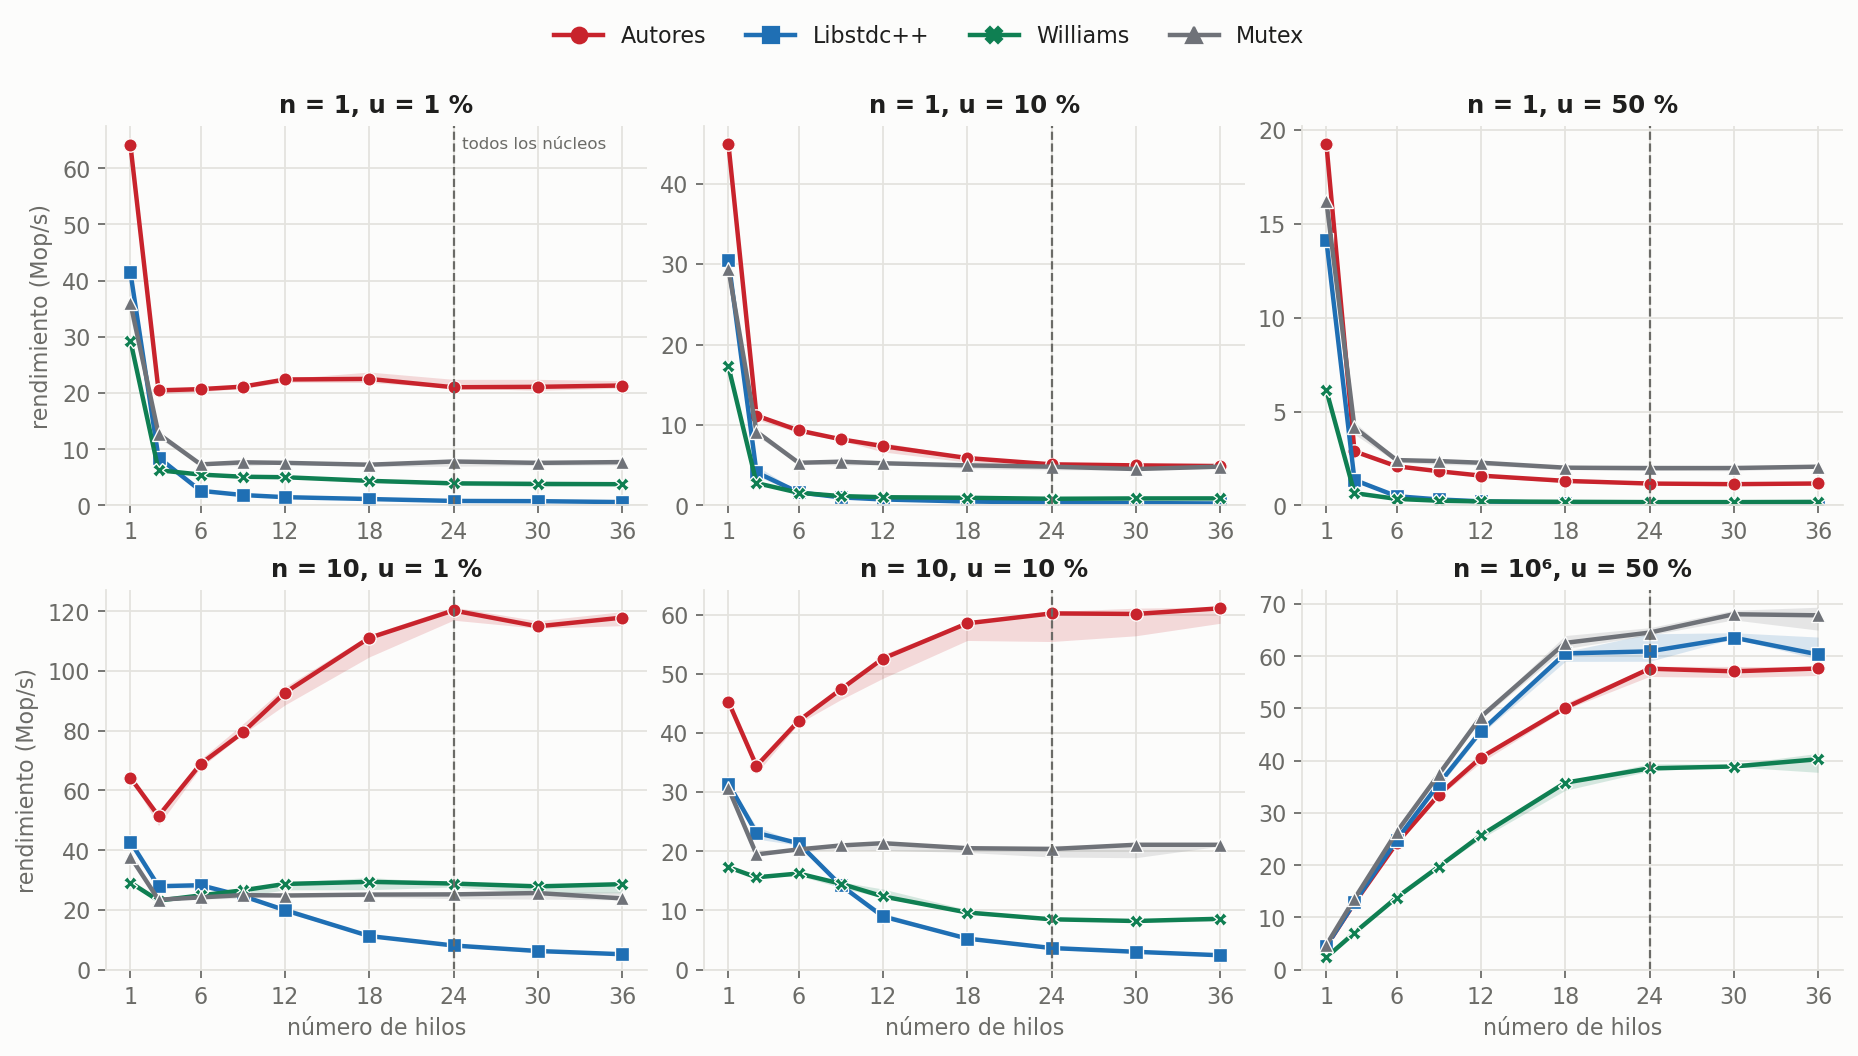
\includegraphics[width=\anchodisponible,height=148pt,keepaspectratio]{figuras/nativo_alineado_fig5.png}\par}}
\note{Figura original de la réplica, tal como la genera analizar.py a partir de los CSV de resultados/david-ultra9-285/. Se explica en la Parte 6.6 de EXPLICACION.md, donde viene también cómo leerla. Úsenla de respaldo en el turno de preguntas.}
\end{frame}}

{\fondo{cF7F4EC}\renewcommand\colorpie{c5F6B7A}\renewcommand\piediapo{\texttt{figuras/docker\_frente\_a\_nativo.png} · generada por analizar.py · se explica en EXPLICACION.md, Parte 6.6}\renewcommand\titulonota{Cada punto de la figura 5, con Docker y sin Docker}
\begin{frame}[plain]
\colocar{t}{{\fontsize{5.69}{7}\selectfont\bfseries\color{cB04A06}\MakeUppercase{Anexo · figura 18 de 20}\par}\vspace{6pt}{\fontsize{11.4}{13.1}\selectfont\bfseries\color{c14213D}\raggedright Cada punto de la figura 5, con Docker y sin Docker\par}\vspace{8pt}{\centering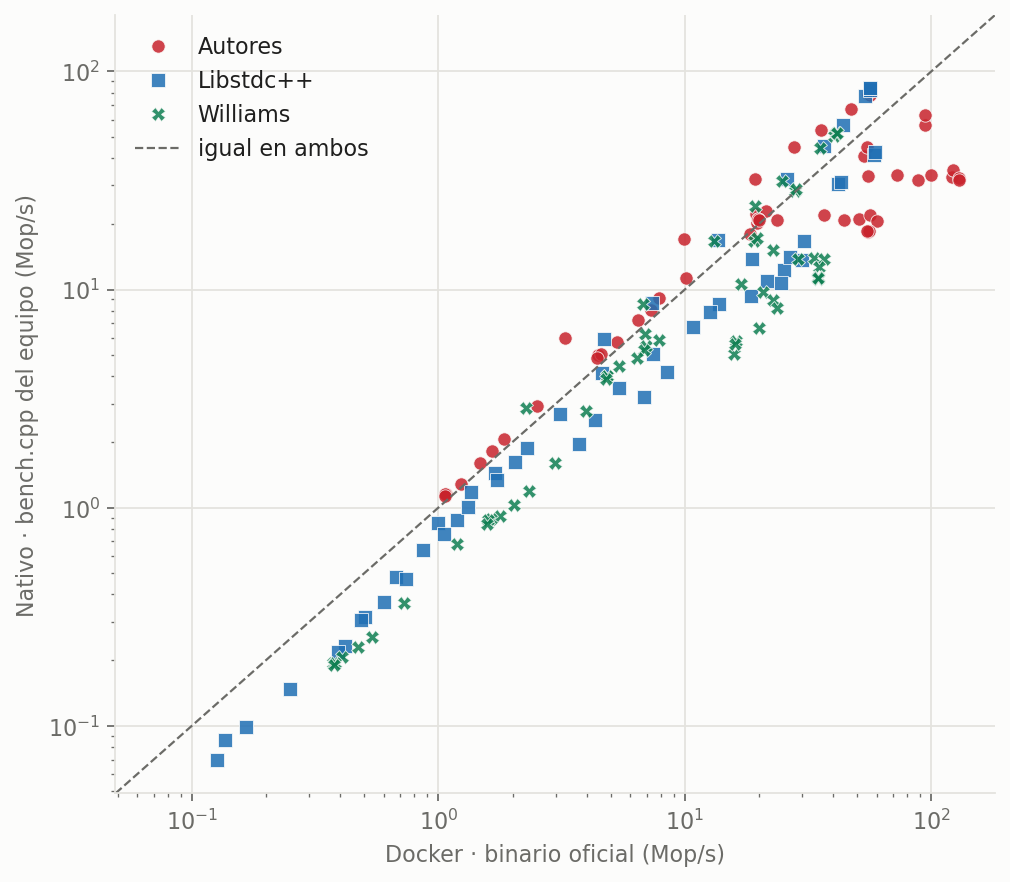
\includegraphics[width=\anchodisponible,height=148pt,keepaspectratio]{figuras/docker_frente_a_nativo.png}\par}}
\note{Figura original de la réplica, tal como la genera analizar.py a partir de los CSV de resultados/david-ultra9-285/. Se explica en la Parte 6.6 de EXPLICACION.md, donde viene también cómo leerla. Úsenla de respaldo en el turno de preguntas.}
\end{frame}}

{\fondo{cF7F4EC}\renewcommand\colorpie{c5F6B7A}\renewcommand\piediapo{\texttt{figuras/nativo\_dosis\_respuesta.png} · generada por analizar.py · se explica en EXPLICACION.md, Parte 6.6}\renewcommand\titulonota{Rendimiento con 4 hilos, de más cerca a más lejos, sin Docker}
\begin{frame}[plain]
\colocar{t}{{\fontsize{5.69}{7}\selectfont\bfseries\color{cB04A06}\MakeUppercase{Anexo · figura 19 de 20}\par}\vspace{6pt}{\fontsize{11.4}{13.1}\selectfont\bfseries\color{c14213D}\raggedright Rendimiento con 4 hilos, de más cerca a más lejos, sin Docker\par}\vspace{8pt}{\centering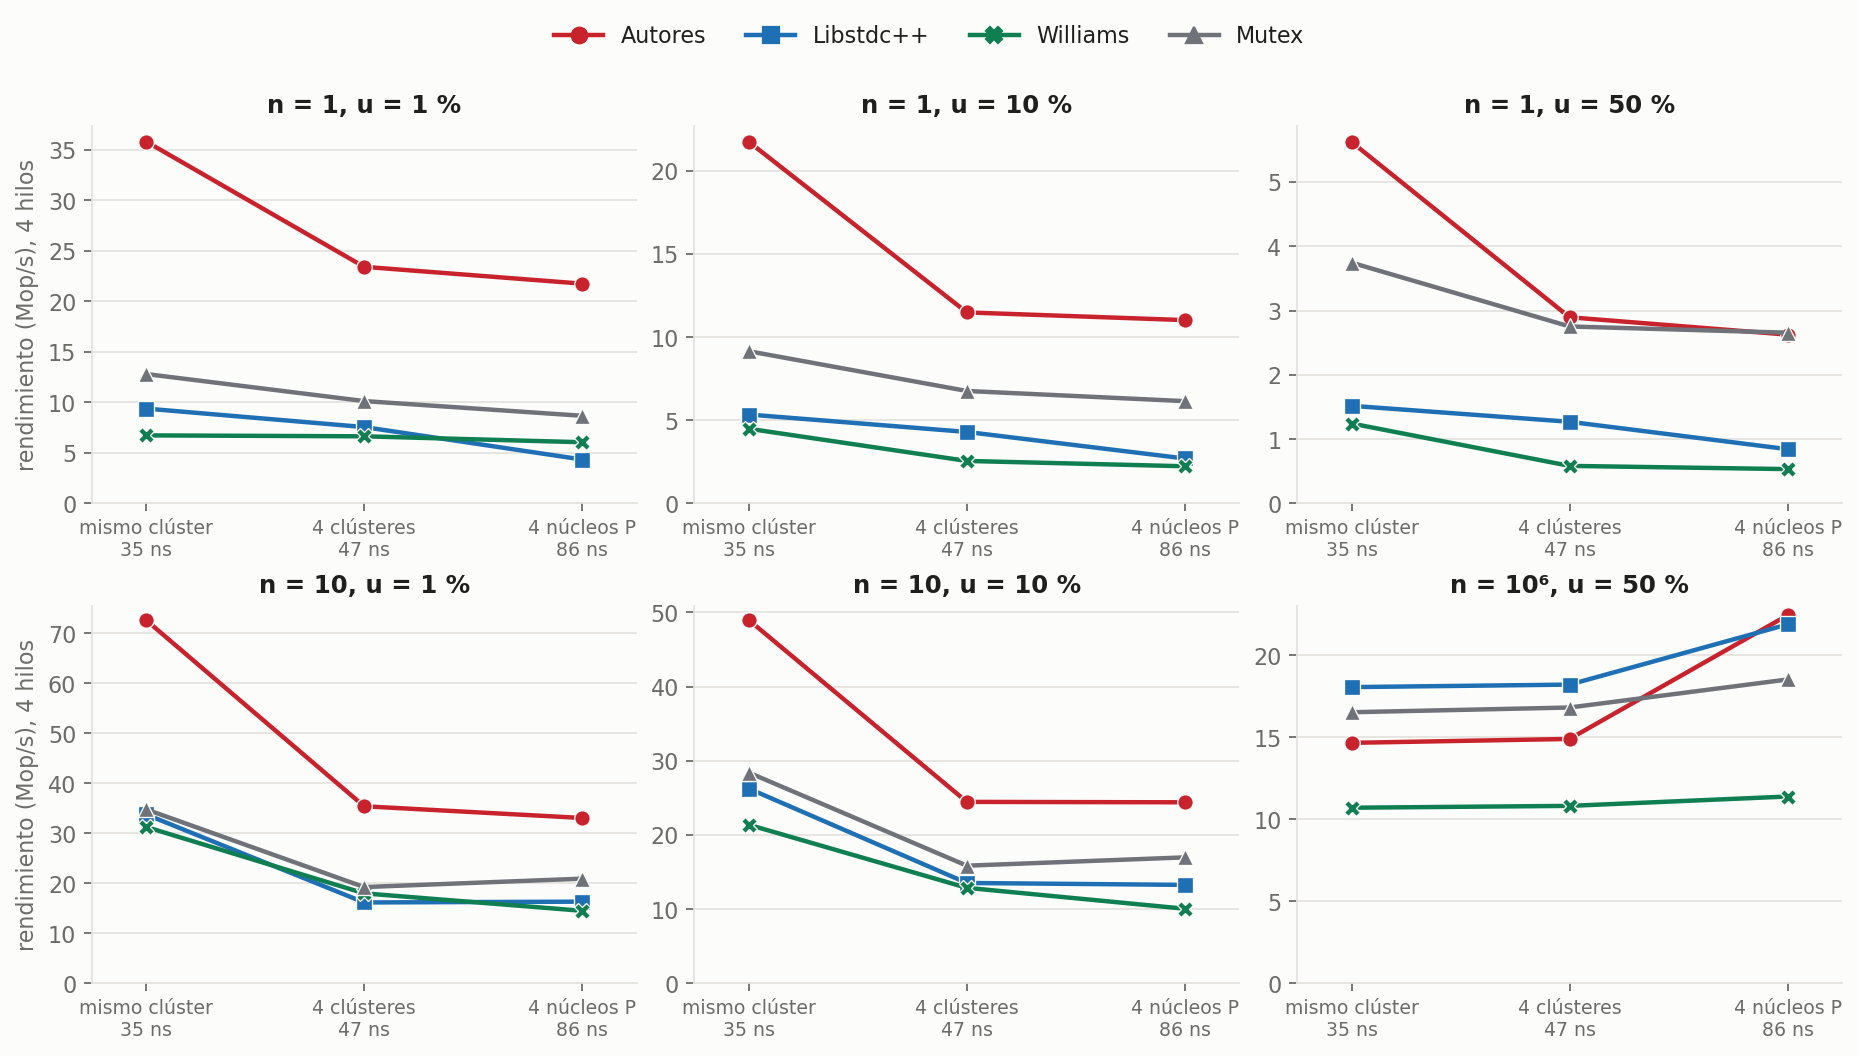
\includegraphics[width=\anchodisponible,height=148pt,keepaspectratio]{figuras/nativo_dosis_respuesta.png}\par}}
\note{Figura original de la réplica, tal como la genera analizar.py a partir de los CSV de resultados/david-ultra9-285/. Se explica en la Parte 6.6 de EXPLICACION.md, donde viene también cómo leerla. Úsenla de respaldo en el turno de preguntas.}
\end{frame}}

{\fondo{cF7F4EC}\renewcommand\colorpie{c5F6B7A}\renewcommand\piediapo{\texttt{figuras/nativo\_fig6.png} · generada por analizar.py · se explica en EXPLICACION.md, Parte 6.6}\renewcommand\titulonota{Latencia sin Docker con bench.cpp del equipo}
\begin{frame}[plain]
\colocar{t}{{\fontsize{5.69}{7}\selectfont\bfseries\color{cB04A06}\MakeUppercase{Anexo · figura 20 de 20}\par}\vspace{6pt}{\fontsize{11.4}{13.1}\selectfont\bfseries\color{c14213D}\raggedright Latencia sin Docker con bench.cpp del equipo\par}\vspace{8pt}{\centering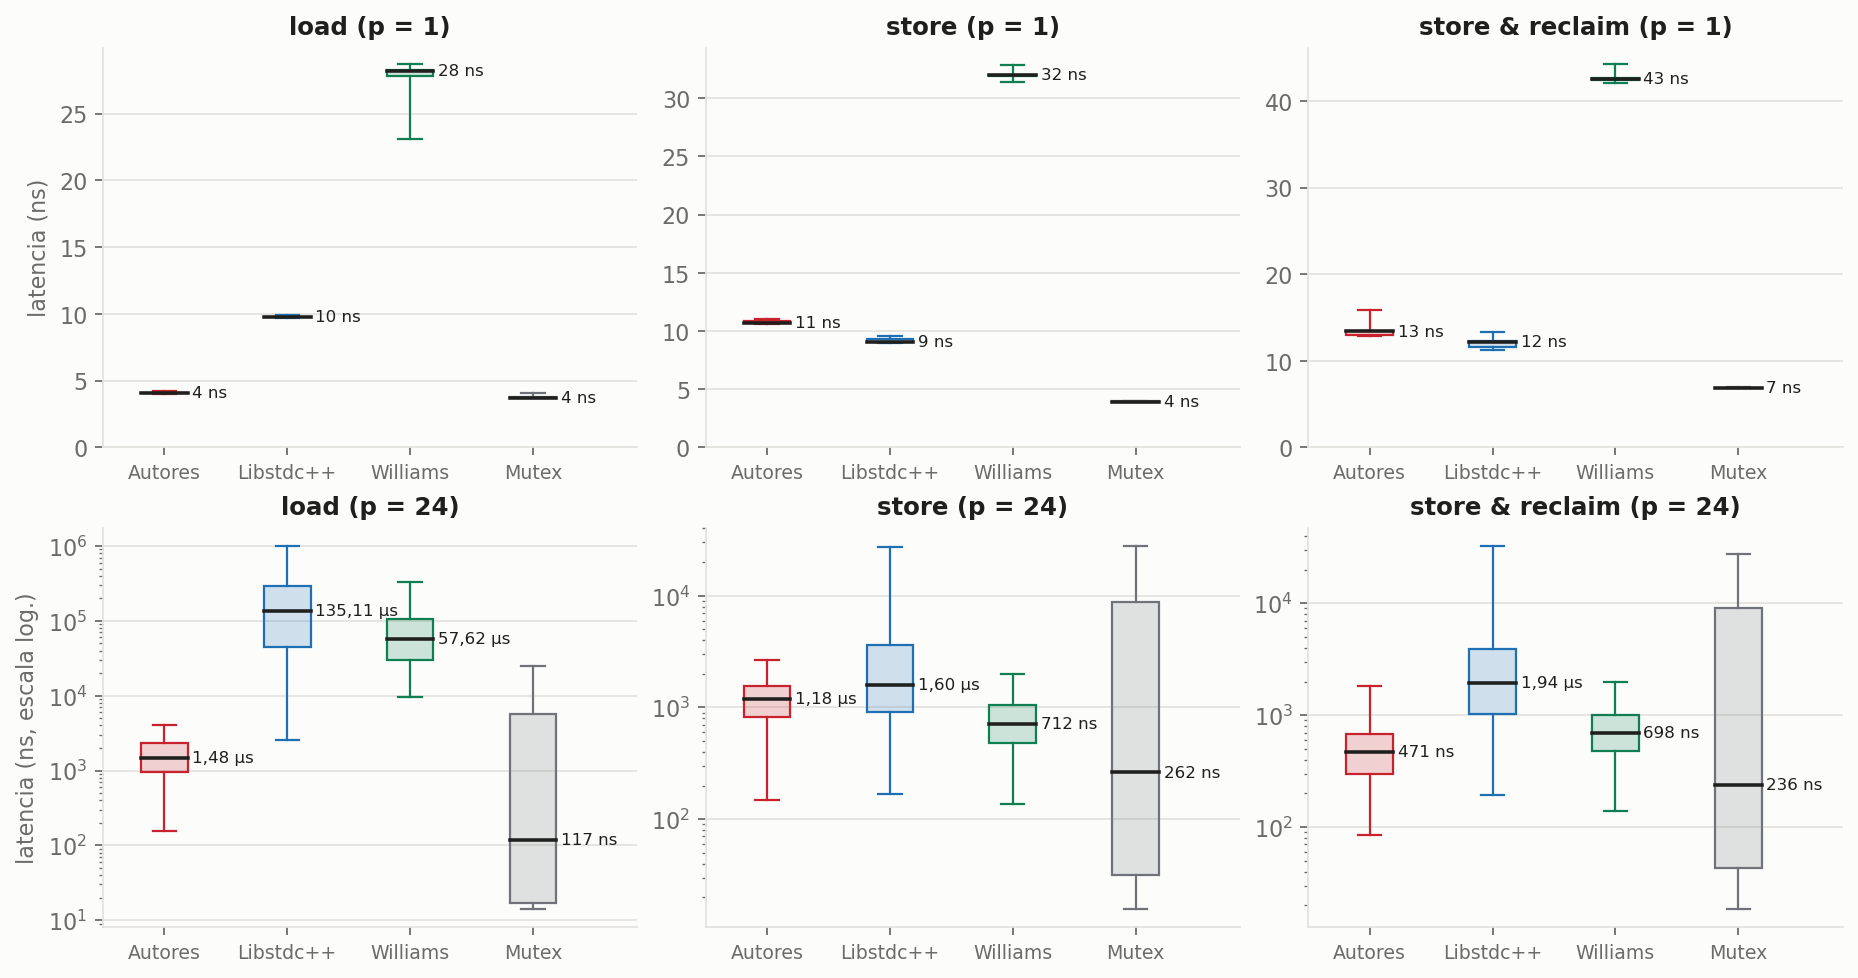
\includegraphics[width=\anchodisponible,height=148pt,keepaspectratio]{figuras/nativo_fig6.png}\par}}
\note{Figura original de la réplica, tal como la genera analizar.py a partir de los CSV de resultados/david-ultra9-285/. Se explica en la Parte 6.6 de EXPLICACION.md, donde viene también cómo leerla. Úsenla de respaldo en el turno de preguntas.}
\end{frame}}
